% Options for packages loaded elsewhere
\PassOptionsToPackage{unicode}{hyperref}
\PassOptionsToPackage{hyphens}{url}
%
\documentclass[
]{article}
\usepackage{amsmath,amssymb}
\usepackage{iftex}
\ifPDFTeX
  \usepackage[T1]{fontenc}
  \usepackage[utf8]{inputenc}
  \usepackage{textcomp} % provide euro and other symbols
\else % if luatex or xetex
  \usepackage{unicode-math} % this also loads fontspec
  \defaultfontfeatures{Scale=MatchLowercase}
  \defaultfontfeatures[\rmfamily]{Ligatures=TeX,Scale=1}
\fi
\usepackage{lmodern}
\ifPDFTeX\else
  % xetex/luatex font selection
\fi
% Use upquote if available, for straight quotes in verbatim environments
\IfFileExists{upquote.sty}{\usepackage{upquote}}{}
\IfFileExists{microtype.sty}{% use microtype if available
  \usepackage[]{microtype}
  \UseMicrotypeSet[protrusion]{basicmath} % disable protrusion for tt fonts
}{}
\makeatletter
\@ifundefined{KOMAClassName}{% if non-KOMA class
  \IfFileExists{parskip.sty}{%
    \usepackage{parskip}
  }{% else
    \setlength{\parindent}{0pt}
    \setlength{\parskip}{6pt plus 2pt minus 1pt}}
}{% if KOMA class
  \KOMAoptions{parskip=half}}
\makeatother
\usepackage{xcolor}
\usepackage[margin=1in]{geometry}
\usepackage{graphicx}
\makeatletter
\def\maxwidth{\ifdim\Gin@nat@width>\linewidth\linewidth\else\Gin@nat@width\fi}
\def\maxheight{\ifdim\Gin@nat@height>\textheight\textheight\else\Gin@nat@height\fi}
\makeatother
% Scale images if necessary, so that they will not overflow the page
% margins by default, and it is still possible to overwrite the defaults
% using explicit options in \includegraphics[width, height, ...]{}
\setkeys{Gin}{width=\maxwidth,height=\maxheight,keepaspectratio}
% Set default figure placement to htbp
\makeatletter
\def\fps@figure{htbp}
\makeatother
\setlength{\emergencystretch}{3em} % prevent overfull lines
\providecommand{\tightlist}{%
  \setlength{\itemsep}{0pt}\setlength{\parskip}{0pt}}
\setcounter{secnumdepth}{-\maxdimen} % remove section numbering
% definitions for citeproc citations
\NewDocumentCommand\citeproctext{}{}
\NewDocumentCommand\citeproc{mm}{%
  \begingroup\def\citeproctext{#2}\cite{#1}\endgroup}
\makeatletter
 % allow citations to break across lines
 \let\@cite@ofmt\@firstofone
 % avoid brackets around text for \cite:
 \def\@biblabel#1{}
 \def\@cite#1#2{{#1\if@tempswa , #2\fi}}
\makeatother
\newlength{\cslhangindent}
\setlength{\cslhangindent}{1.5em}
\newlength{\csllabelwidth}
\setlength{\csllabelwidth}{3em}
\newenvironment{CSLReferences}[2] % #1 hanging-indent, #2 entry-spacing
 {\begin{list}{}{%
  \setlength{\itemindent}{0pt}
  \setlength{\leftmargin}{0pt}
  \setlength{\parsep}{0pt}
  % turn on hanging indent if param 1 is 1
  \ifodd #1
   \setlength{\leftmargin}{\cslhangindent}
   \setlength{\itemindent}{-1\cslhangindent}
  \fi
  % set entry spacing
  \setlength{\itemsep}{#2\baselineskip}}}
 {\end{list}}
\usepackage{calc}
\newcommand{\CSLBlock}[1]{\hfill\break\parbox[t]{\linewidth}{\strut\ignorespaces#1\strut}}
\newcommand{\CSLLeftMargin}[1]{\parbox[t]{\csllabelwidth}{\strut#1\strut}}
\newcommand{\CSLRightInline}[1]{\parbox[t]{\linewidth - \csllabelwidth}{\strut#1\strut}}
\newcommand{\CSLIndent}[1]{\hspace{\cslhangindent}#1}
\usepackage{helvet}
\renewcommand*\familydefault{\sfdefault}
\usepackage{setspace}
\doublespacing
\usepackage[left]{lineno}
\linenumbers
\usepackage{booktabs}
\usepackage{longtable}
\usepackage{array}
\usepackage{multirow}
\usepackage{wrapfig}
\usepackage{float}
\usepackage{placeins}
\usepackage{colortbl}
\usepackage{pdflscape}
\usepackage{tabu}
\usepackage{threeparttable}
\usepackage{threeparttablex}
\usepackage[normalem]{ulem}
\usepackage{makecell}
\usepackage{xcolor}
\usepackage{caption}
\usepackage[labelformat=empty]{caption}
\usepackage{multirow}
\usepackage{multicol}
\usepackage{colortbl}
\usepackage{hhline}
\newlength\Oldarrayrulewidth
\newlength\Oldtabcolsep
\usepackage{longtable}
\usepackage{array}
\usepackage{hyperref}
\usepackage{float}
\usepackage{wrapfig}
\ifLuaTeX
  \usepackage{selnolig}  % disable illegal ligatures
\fi
\usepackage{bookmark}
\IfFileExists{xurl.sty}{\usepackage{xurl}}{} % add URL line breaks if available
\urlstyle{same}
\hypersetup{
  pdftitle={Characterizing the Transcriptome of Turkey Hemorrhagic Enteritis Virus in a Turkey B-cell Line},
  hidelinks,
  pdfcreator={LaTeX via pandoc}}

\title{Characterizing the Transcriptome of Turkey Hemorrhagic Enteritis
Virus in a Turkey B-cell Line}
\author{}
\date{\vspace{-2.5em}}

\begin{document}
\maketitle

\captionsetup[table]{labelformat=empty}

\vspace{5mm}

\textbf{Running Title:} Novel Insights into Turkey Hemorrhagic Enteritis
Virus Transcriptome

\vspace{10mm}

Abraham Quaye\textsuperscript{1*}, Brett E. Pickett\textsuperscript{*},
Joel S. Griffitts\textsuperscript{*}, Bradford K.
Berges\textsuperscript{*}, Brian D.
Poole\({^\dagger}\)\textsuperscript{*}

\vspace{5mm}

\textsuperscript{*}Department of Microbiology and Molecular Biology,
Brigham Young University\\
\textsuperscript{1}First-author\\
\({^\dagger}\) Corresponding Author

\vspace{5mm}

\textbf{Corresponding Author Information}\\
\href{mailto:brian_poole@byu.edu}{\nolinkurl{brian\_poole@byu.edu}}\\
Department of Microbiology and Molecular Biology,\\
4007 Life Sciences Building (LSB),\\
Brigham Young University,\\
Provo, Utah\\
\newpage

\subsection{ABSTRACT}\label{abstract}

Characterizing the splice map of turkey hemorrhagic enteritis virus
(THEV) is an essential step that would allow studies of individual genes
mediating its immunosuppressive functions. We used an RNA-sequencing
experiment to characterize the transcriptome of THEV for the first time,
providing key insight into the THEV gene expression and mRNA structures.
Researchers previously annotated THEV's genome as encoding 23 open
reading frames (ORFs). In this work we identified 29 spliced transcripts
all of which consisted of novel exons although some exons matched some
previously annotated ORFs. The three annotated splice junctions were
also corroborated by our data. We performed PCR amplification of THEV
cDNA, cloned the PCR products, and used Sanger sequencing to validate
all identified splice junctions. During validation we identified five
additional unique transcripts, a subset of which were further validated
by 3' rapid amplification of cDNA ends (3' RACE) experiments. Thus, we
report that the genome of THEV contains 34 unique transcripts with the
coding capacity for all annotated ORFs. However, we found six of the
previously annotated ORFs (ORF1, E3, 33K, ORF8, IVa2, and protease) to
be truncated ORFs on the basis of the identification of an in-frame
upstream start codon or the detection of additional coding exons. We
also identified three of the annotated ORFs with longer or shorter
isoforms, and seven novel unpredicted ORFs that could potentially be
translated; although it is beyond the scope of this manuscript to
investigate whether they are translated. Similar to other adenoviruses
(AdVs), THEV also produces multiple distinctly spliced transcripts that
code for the same proteins across its genome. Our data show that all
THEV transcripts are spliced and organized into five transcription units
under the control of their cognate promoters like other AdVs. However,
our data suggest that the temporal regulation of THEV may be different
from other AdVs. \newpage

\subsection{INTRODUCTION}\label{introduction}

Adenoviruses (AdVs) are non-enveloped icosahedral-shaped DNA viruses,
causing infection in virtually all types of vertebrates studied to date.
Their double-stranded linear DNA genomes range between 26 and 45kb in
size, producing a broad repertoire of transcripts via highly complex
alternative splicing patterns (1, 2). The AdV genome is one of the most
optimally economized; both the forward and reverse DNA strands harbor
protein-coding genes, making it highly gene-dense. There are 16 genes
termed ``genus-common'' that are homologous in all AdVs; these are
thought to be inherited from a common ancestor. All other genes are
termed ``genus-specific''. The genus-specific genes tend to be located
at the termini of the genome while genus-common genes are usually
towards the center of the genome (1). This pattern is also observed in
\emph{Poxviridae} and \emph{Herpesviridae}, which also have linear DNA
genomes (1, 3, 4). The family \emph{Adenoviridae} consists of five
genera: \emph{Mastadenovirus} (MAdV), \emph{Aviadenovirus},
\emph{Atadenovirus}, \emph{Ichtadenovirus}, and \emph{Siadenovirus}
(SiAdV) to which turkey adenovirus 3 also called turkey hemorrhagic
enteritis virus (THEV) belongs (5--10). Members of SiAdV have the
smallest genome size (\textasciitilde26 kb) and gene content of all
known AdVs (see \textbf{Figure 1}) (1, 2, 6).

Virulent THEV strains (THEV-V) and avirulent strains (THEV-A) of THEV
both infect turkeys, with THEV-V causing hemorrhagic enteritis (HE), a
debilitating acute disease predominantly affecting turkey poults
characterized by immunosuppression (IS), intestinal lesions leading to
bloody diarrhea, and up to 80\% mortality (2, 11--13). While the current
vaccine strain (a THEV-A strain isolated from a pheasant; Virginia
Avirulent Strain {[}VAS{]}) has proven effective at preventing HE in
turkey poults, it still retains its immunosuppressive ability. Thus,
vaccinated birds are rendered more susceptible to opportunistic
infections and death than unvaccinated birds leading to substantial
economic losses (11, 14--16). To eliminate the immunossupressive effect
of the vaccine strain, a thorough investigation of the culprit viral
genes mediating this phenomenon is essential. However, the transcriptome
(splicing and gene expression patterns) of THEV has not been
characterized, making an investigation of specific IS-related viral
genes impractical.

A myriad of studies have elucidated the AdV transcriptome in fine detail
(17, 18). However, a large preponderance of studies focus on MAdVs --
specifically human AdVs. Thus, most of the current knowledge regarding
AdV gene expression and replication is based on MAdV studies, which is
generalized for all other AdVs (10, 19). MAdV transcription is
temporally regulated; therefore, genes are categorized into five early
transcription units (E1A, E1B, E2, E3, and E4), two intermediate (IM)
units (pIX and IVa2), and one major late transcription unit (MLTU or
major late promoter {[}MLP{]} region), which generates five families of
late mRNAs (L1-L5) based on the polyadenylation site. An additional gene
(UXP or U exon) is located on the reverse strand. The early genes encode
non-structural proteins such as enzymes or host-cell modulating
proteins, primarily involved in DNA replication, or providing the
necessary intracellular niche for optimal replication while late genes
encode structural proteins that act as capsid proteins, promote virion
assembly, or direct genome packaging. The immediate early genes E1A are
expressed first, followed by the delayed early genes, E1B, E2, E3 and
E4. Then the intermediate early genes, IVa2 and pIX are expressed
followed by the late genes (10, 17, 18). It is noteworthy that the MLP
shows basal transcriptional activity during early infection (before DNA
replication), with a comparable efficiency to other early viral
promoters, but it reaches its maximal activity during late infection
(after DNA replication). However, during early infection only a subset
of the MLP-derived transcripts are expressed (10). MAdV makes an
extensive use of alternative RNA splicing to produce a very complex
array of mRNAs. All but the pIX mRNA undergo at least one splicing
event. For instance, the MLTU produces over 20 distinct splice variants
all of which contain three non-coding exons at the 5'-end (collectively
known as the tripartite leader; TPL) (17, 18). There is also an
alternate three-exon 5' non-coding leader sequence present in varying
amounts on a subset of MLTU mRNAs (known as the x-, y-, and z-leaders).
Lastly, there is the i-leader exon, which is infrequently included
between the second and third TPL exons, and codes for the i-leader
protein (20). Thus, the MLTU produces a complex repertoire of mRNA with
diverse 5' untranslated regions (UTRs) spliced onto different 3' coding
exons which are grouped into five different 3'-end classes (L1-L5) based
on polyadenylation site. Each transcription unit (TU) contains its own
promoter driving the expression of the array of mRNA transcripts
produced via alternative splicing in the unit (10, 17, 18). The
promoters are activated at different phases of the infection by proteins
from previously activated TUs. Paradoxically, the early-to-late phase
transition during infection requires the L4 gene products, 22K and 33K,
which should only be available after the transition. However, a promoter
in the L4 region (L4P) that directs the expression of these two proteins
independent of the MLP was found, resolving the paradox (10, 17, 21).
During translation of AdV mRNA, recent studies using long-read direct
RNA sequencing strongly suggest the potential usage of secondary start
codons; adding to what was already a highly complex system for gene
expression (17, 22).

High throughput sequencing methods have facilitated the discovery of
many novel transcribed regions and splicing isoforms. It is also a very
powerful tool to study alternative splicing under different conditions
at an unparalleled depth (18, 22, 23). In this paper, we use a
paired-end deep sequencing experiment to characterize, for the first
time, the transcriptome and splicing of THEV (VAS vaccine strain) during
different phases of the infection. Our paired-end sequencing allowed for
reading 149 bp long high quality (mean Phred Score of 36) sequences from
each end of cDNA fragments, which were mapped to the genome of THEV.
\newpage

\subsection{RESULTS}\label{results}

\textbf{Overview of sequencing data and analysis pipeline outputs}\\
A previous study by Aboezz \emph{et al} showed that almost all THEV
transcripts were detectable beginning at 4 hours, with a full
replication cycle of about 18-hours post infection (hpi) (24).
Therefore, infected MDTC-RP19 cells were harvested at 4-, 12-, 24-, and
72-hpi to ensure a wide time window to sample all transcripts. Our
paired-end RNA sequencing (RNA-seq) experiment yielded an average of
107.1 million total reads of 149 bp in length per time-point, which were
simultaneously mapped to both the virus (THEV) and host (\emph{Meleagris
gallopavo}) genomes using the Hisat2 (25) reference-based aligner. A
total of 18.1 million reads from all time-points mapped to the virus
genome; this provided good coverage/depth, leaving no regions unmapped.
The mapped reads to the virus genome increased substantially from a mere
432 reads at 4 hpi to 16.9 million reads at 72 hpi (\textbf{Table 1},
\textbf{Figure 2A}). From the mapped reads, we identified a total of
2,457 unique THEV splice junctions from all time-points, with splice
junctions from the later time-points being supported by significantly
more sequence reads than earlier time-points. For example, all the 13
unique junctions at 4 hpi had less than 10 reads supporting each one,
averaging a mere 2.8 reads per junction. Conversely, the 2374 unique
junctions at 72 hpi averaged 898.4 reads per junction, some junctions
having coverage as high as 322,677 reads. The substantial increases in
splice junction and mapping reads to the THEV genome over time denotes
an active infection and a successful viral replication, and correlates
with our quantitative PCR (qPCR) assay quantifying the total number of
viral genome copies over time (\textbf{Figure 2B}).

Using StringTie (25), we assembled the data into potential transcripts
using the genomic location of the prior predicted THEV ORFs as a guide.
In the consolidated transcriptome, a composite of all non-redundant
transcripts from all time points, we counted a total of 29 novel
transcripts. We found that a subset of exons in the viral transcripts
match the predicted ORFs exactly, with the majority of the exons being
longer and spanning multiple predicted ORFs (\textbf{Figure 3}).

We then validated the splice junctions in all transcripts by PCR
amplification of viral cDNA, cloning, and Sanger sequencing
(\textbf{Supplementary PCR methods}). During validation, we identified
five additional transcripts, some of which were further validated by 3'
Rapid Amplification of cDNA Ends (3' RACE) data. The complete list of
unique splice junctions mapped to the THEV genome has been submitted to
the National Center for Biotechnology Information Gene Expression
Omnibus (\url{http://www.ncbi.nlm.nih.gov/geo}) under accession number
GSE254416.

\textbf{Changes in THEV splicing profile over time}\\
AdV gene expression occurs under exquisite temporal control with each
promoter typically producing one or few pre-mRNAs that undergo
alternative splicing to yield a repertoire of mature mRNAs. To evaluate
the activity of each promoter over time, StringTie and Ballgown (a
program for statistical analysis of assembled transcriptomes) (26) were
used to estimate the normalized expression levels of all transcripts for
each time point in Fragments Per Kilobase of transcript per Million
mapped reads (FPKM) units. Very few unique splice junctions, reads, and
transcripts were counted at 4 hpi; hence, this time point was excluded
in this analysis.

Considering individual mRNAs, TRXPT\_21 -- from the E2 region -- was the
most significantly expressed at 12 hpi, constituting 33.58\% of the
total expression of all transcripts. Transcripts in the E3 and E4
regions also contributed significant proportions, and noticeably, some
MLP region transcripts. The later time points were dominated by the MLP
region transcripts -- TRXPT\_10 and TRXPT\_14 were the most abundantly
expressed at 24 and 72 hpi, respectively, as expected (\textbf{Figure
4A}). When we performed analysis of the FPKM values of transcripts per
region we found a similar pattern: the E2 region was the most abundantly
expressed at 12 hpi, after which the MLP region assumes predominance
(\textbf{Figure 4B}). Secondly, we estimated relative abundances of all
splice junctions at each time point using the raw reads. Only junctions
with a read coverage of at least 1\% of the total splice junction reads
at the given time point were considered significant and included in
\textbf{Tables 2a-2c}. At 12 hpi, 18 junctions meet the 1\% threshold,
and were comprised of predominantly early region (E1, E2, E3, and E4)
junctions, albeit the MLTU was the single most preponderant region
overall, constituting 38.8\% of all the junction reads (\textbf{Table
2a} and \textbf{Supplementary Table S1a}). The most abundant junctions
at 12 hpi remained the most significantly expressed at 24 hpi also.
However, here, the MLP-derived junctions were unsurprisingly even more
preponderant overall, accounting for 45.7\% of all the junction reads
counted (\textbf{Table 2b} and \textbf{Supplementary Table S1b}). At 72
hpi, the trend of increased activity of the MLP continued as expected;
at this time, the MLP region junctions were not only the most abundant
overall -- accounting for 67.3\% of all junction reads, -- but also
contained the most significantly expressed individual junctions
(\textbf{Table 2c}, \textbf{Supplementary Table S1c} and \textbf{Figure
4C}). When we limited this analysis to only junctions in the final
transcriptome, we observed the relative abundances of the junctions for
each region over time to be similar to the pattern seen with all the
junctions included (\textbf{Figure 4D}).

We also analyzed splice donor and acceptor site nucleotide usage over
time to investigate any peculiarities that THEV may show, generally or
over the course of the infection. We found that most splice
donor-acceptor sequences were unsurprisingly the canonical GU-AG
nucleotides. However, the splice acceptor-donor pairing became less
specific over time, such that all combinations of nucleotide pairs were
eventually detected (\textbf{Figure 5}).

\textbf{Early Region 1 (E1) transcripts}\\
This region in MAdVs is the first transcribed after successful entry of
the viral DNA into the host cell nucleus, albeit at low levels (18). The
host transcription machinery solely mediates the transcription of this
region. After their translation, the E1 proteins in concert with a
myriad of host transcription factors activate other viral promoters
(10). In MAdVs, this region is subdivided into E1a and E2b units, but
the transcripts found in our data categorized under this region do not
appear to be subdivided.

Only two ORFs (ORF1 {[}sialidase{]} and Hyd) are predicted in this
region; however, we discovered four novel transcripts in this region,
which collectively contain 3 unique splice junctions (\textbf{Figure
6}). Most of the ORFs of the novel transcripts are distinct from the
predicted ORFs, but they all have the coding potential (CP) for the
predicted Hyd protein as the 3'-most coding sequence (CDS) if secondary
start codon usage is considered as reported for other AdVs (17, 18). The
5'-most CDS of TRXPT\_1 is multi-exonic, encoding a novel 17.9
kilodalton (kDa), 160 residue {[}amino acids (aa){]} protein (ORF9).
From its 5'-most start codon (SC), TRXPT\_2 encodes the largest protein
in this region -- a 64.3 kDa, 580 aa protein (ORF10) with the same SC as
ORF9 (position 211 bp). ORF10 spans almost the entire predicted ORF1 and
Hyd, coming short in two regards: it is spliced from 1655 bp to 1964 bp
(ORF1's C-terminus, including the stop codon), and its stop codon (STC;
position 2312) is 13 bp short of the Hyd STC. However, it has an SC 102
bp upstream and in-frame with ORF1's predicted SC. Thus, ORF10 shares
substantial protein sequence similarity with ORF1 but not with Hyd, as
the SC of Hyd is not in-frame. Without its splice site removing the ORF1
STC, TRXPT\_2 would encode a longer variant of ORF1, starting from an
upstream SC. TRXPT\_3 is almost identical to TRXPT\_1, except for the
lack of TRXPT\_1's second exon. Our RNA-seq data show that all E1
transcripts share the same transcription termination site (TTS; at
position 2325 bp). However, TRXPT\_3 and TRXPT\_4 seem to have
transcription start sites (TSS) downstream of the TSS of TRXPT\_1 and
TRXPT\_2 (E1 TSS; position: 54 bp). Given that studies in MAdVs show
that E1 mRNAs share not only a common TTS but also the TSS, and only
differ from each other regarding the internal splicing (18), it is
likely that TRXPT\_3 and TRXPT\_4 are incomplete, and their actual TSS
just like the TTS are identical for all E1 transcripts. Regardless of
the TSS considered for TRXPT\_3, the CP remains unaffected. Its 5'-most
CDS, beginning at 1965 bp and sharing the same STC as ORF9, produces a
13.1 kDa, 115 residue protein (ORF4). ORF4 was predicted in an earlier
study (27) but was excluded in later studies (1, 12); however, our data
suggest it is a genuinely expressed ORF. Unlike TRXPT\_3, the CP of
TRXPT\_4 is affected by the TSS considered; if we consider its
unmodified TSS, then its CP is identical to TRXPT\_3. However, if we
assume that TRXPT\_4 uses the E1 TSS, then the 5'-most CDS is a
distinct, novel, multi-exonic 15.9 kDa, 143 aa protein (ORF11) with the
same SC as ORF9 and ORF10 but with a unique STC.

The splice junctions of all transcripts in this region (except the
junction for TRXPT\_4) were validated by cloning of viral cDNA and
Sanger sequencing (\textbf{Supplementary PCR methods}). During the
validation of TRXPT\_2, we found ORF1 to be present on the agarose gel
(an unspliced band size) and Sanger sequencing results showed it to be a
transcribed mRNA (\textbf{Supplementary PCR methods}). This was
corroborated by our 3' RACE experiment, which showed a transcript
(TRXPT\_2B) spanning the entire ORF1 and Hyd ORFs without any splicing,
with a poly-A tail immediately after the E1 TTS. The 5'-most CDS of this
transcript (TRXPT\_2B) would encode ORF1. However, TRXPT\_2B has an
upstream and in-frame SC to the predicted SC of ORF1, suggesting that
the predicted ORF1 CDS is truncated -- the actual ORF1 (eORF1) that is
expressed shares the same SC as ORF10, but has a unique STC.

\textbf{Early Region 2 (E2) and Intermediate Region (IM) transcripts}\\
The E2 TU expressed on the anti-sense strand is subdivided into E2A and
E2B and encodes three classical AdV proteins -- pTP and Ad-pol (E2B
proteins), and DBP (E2A protein) -- essential for genome replication
(17, 18). Unlike MAdV where two promoters (E2-early and E2-late) are
known (17), we discovered only a single TSS (E2 TSS; 18,751 bp) from
which both E2A and E2B transcription is initiated. However, similar to
MAdVs, E2A and E2B transcripts have distinct TTSs, and the E2B
transcripts share the TTS of the IVa2 transcript of the IM region (17,
18) (\textbf{Figure 7}).

The E2A ORF, DBP is one of three THEV ORFs predicted to be spliced from
two exons. The corresponding transcript (TRXPT\_21) found in our data
matches this predicted splice junction precisely but with a non-coding
additional exon at the 5'-end (E2-5'UTR) at position 18,684-18,751 bp.
Thus, TRXPT\_21 is a three-exon transcript encoding DBP (380 residues,
43.3 kDa) precisely as predicted. This transcript (TRXPT\_21) was also
corroborated in a 3' RACE experiment. Additionally, from the 3' RACE
data, we found a splice variant of TRXPT\_21 which retains the second
intron leading to a 2-exon transcript. This new transcript (TRXPT\_21B),
albeit longer due to retaining the second intron and possessing a short
3' UTR, encodes a truncated isoform of DBP (tDBP) because the SC
utilized by TRXPT\_21, is followed shortly by STCs in the retained
intron. The SC 173 bp downstream of the DBP SC yields tDBP (a 346
residue, 39.3 kDa product), which is in-frame of DBP but entirely
contained in the second exon. TRXPT\_21 and TRXPT\_21B share a common
TTS but TRXPT\_21B as seen in our 3'-RACE data, extends 39 bp into an
adenine/thymine (A/T)-rich sequence before the poly-A tail sequence
occurs, suggesting this position (16,934 bp) as the true E2A TTS
(\textbf{Figure 7}).

The E2B region transcripts also start with the E2-5'UTR but extend
thousands of base pairs downstream to reach the TTS at 2334 bp in the IM
region, which is immediately followed by an A/T-rich sequence (position
2323-2339 bp) where polyadenylation probably occurs. Interestingly, the
TTS of the E1 region (position 2,325 bp) on the sense strand is also in
the immediate vicinity of this A/T-rich sequence, which is almost
palindromic; hence it likely serves as the polyadenylation signal for
both E1 and E2B/IM transcripts. The E2B transcripts TRXPT\_6 and
TRXPT\_7 are almost identical except for an extra splice junction at the
3'-end of TRXPT\_6, making TRXPT\_6 a five-exon transcript and TRXPT\_7,
four exons (\textbf{Figure 7}). TRXPT\_7 has the CP for both classical
proteins (pTP and Ad-pol) encoded in this region, of which the pTP ORF
is predicted to be spliced from two exons just like in all other AdVs.
The predicted splice junction of pTP is corroborated by our data;
however, the full transcript is markedly longer than the predicted ORF:
there are two novel non-coding 5' exons, the third exon (containing the
SC of pTP) is significantly longer than predicted, and the last exon
containing the bulk of the CDS is more than triple the predicted size of
pTP. The first two exons are 5'-UTRs because the SC here is immediately
followed by STCs; thus, the 5'-most SC (position 10,995 bp) of the third
exon which matches the predicted SC of pTP is utilized. The encoded
product is identical to the predicted pTP protein (597 residues; 70.5
kDa). If secondary SC (secSC) usage is considered, with SC at 6768 bp
and STC at 3430 bp, the encoded product is identical to the predicted
Ad-pol (polymerase) protein (1112 residues; 129.2 kDa). TRXPT\_6 differs
from TRXPT\_7 by containing an extra splice site at 3447-3515 bp.
However, the CP remains similar to that of TRXPT\_7 except the Ad-pol
encoded from the secSC is a truncated isoform with a new STC resulting
from the splice site.

While both TRXPT\_6 and TRXPT\_7 have the CP for Ad-pol with secSC
usage, in all AdVs studied, the two proteins (pTP and Ad-pol) are
encoded by separate mRNAs with identical first three 5' exons and TTS,
but the splice junction to the terminal exons are different. We checked
for a longer splice junction between the third and fourth (terminal)
exons of TRXPT\_7 with our junction validation method (targeted PCR,
cloning, and Sanger sequencing) and discovered a unique splice junction
(10,981-7062 bp) not found in our RNA-seq data. If initiated from the E2
TSS and terminated at the E2 TTS, this transcript (TRXPT\_31) would
encode Ad-pol exactly as predicted as its 5'-most CDS (\textbf{Figure
7}).

Our RNA-seq data also showed a novel short transcript (TRXPT\_15)
entirely nested within the terminal exon of TRXPT\_7 but with a unique
splice site. This transcript is an incomplete construction from the
mapped reads as it contains a truncated CDS. However, we validated this
splice junction to be genuine (\textbf{Supplementary PCR methods}).

The IM region is a single-transcript TU, encoding a single classical
protein, IVa2. The promoter expressing this single transcript (TRXPT\_5)
is embedded in E2B region and shares a TTS with E2B transcripts (17,
18). TRXPT\_5 is a two-exon transcript spliced exactly as the last
splice junction of TRXPT\_6. The first exon is a UTR, except the last 2
nucleotides, which connect with the first nucleotide of the second exon
to form the 5'-most SC. This first SC is 4 codons upstream and in-frame
of the predicted IVa2 SC. Except for the four extra N-terminus residues,
the entire protein sequence is identical to the predicted IVa2.

\textbf{Early Region 3 (E3) transcripts}.\\
The E3 region is wholly contained in the MLTU and encodes proteins
involved in modulating and evading the host immune defenses. In MAdVs,
this region contains seven ORFs expressed from several transcripts which
share the same TSS (from the E3 promoter) but have different TTSs (10,
17, 18). However, some E3 transcripts use the TSS of the MLP. Due to
sharing the same TSS, in MAdVs, secSC usage is heavily relied on for
gene expression in this region except for 12.5K and transcripts using
the MLP TSS, as utilizing only the first SC cannot produce all the other
transcripts in this TU (17).

In THEV, only one ORF (E3) was predicted in this region. However, as the
E3 TU is nested in the MLTU, transcripts from the L4P (100K, 22K, 33K,
and pVIII) not only overlap the E3 region transcripts entirely as seen
in our RNA-seq results, but also have their TSS and TTS in practically
the same locations (\textbf{Figure 8}). Therefore, we have categorized
these two groups together as E3 transcripts.

We identified seven novel transcripts here (TRXPT\_22, TRXPT\_23,
TRXPT\_24, TRXPT\_25, TRXPT\_26, TRXPT\_27, TRXPT\_29) from our RNA-seq
data, all originating from two distinct TSSs -- we consider the first
TSS (position 18,230 bp) as corresponding to the L4P and the other at
18,727 bp as corresponding to the E3 promoter (E3P). These E3
transcripts collectively have the CP for several predicted THEV ORFs:
100K, 22K, 33K, pVIII, and E3, as well as Fiber (IV) and ORF7 belonging
to the MLTU. But some of these CDSs are different than predicted due to
either unknown exons or the presence of an in-frame upstream SC. For
instance, 33K is one of the few THEV ORFs predicted to be spliced from
two exons; however, we discovered a significantly longer four-exon ORF
(e33K) on TRXPT\_24 that contains it almost entirely. The first two
exons of e33K were not predicted but the last two match the predicted
exons and the CDS is in-frame, albeit the first 20 bp of the predicted
33K (including the SC at 20,142 bp) is spliced out as part of the second
intron of TRXPT\_24. Thus, the bona fide 33K (e33K) is a 19.8 kDa, 171
residue protein spanning four exons instead of the predicted 120 aa
protein. TRXPT\_24 also has the CP for pVIII and E3 if we consider
downstream SC usage. However, the predicted E3 has an upstream in-frame
SC; thus, this longer version of E3 (eE3) is likely the genuinely
expressed ORF. TRXPT\_29 is the shortest transcript in this TU. It is a
two-exon transcript, both exons comprising the CDS. The product of
TRXPT\_29 is a novel 73 residue protein (8.3KI) sharing the SC of e33K
but with a unique STC. TRXPT\_23 being spliced identically as TRXPT\_29
also encodes 8.3KI from its first SC. Similarly, TRXPT\_22 also encodes
a 73 aa novel protein (8.3KII) from its first SC that shares over 80\%
similarity with 8.3KI, but it differs from 8.3KI at the C-terminus.
Considering downstream SC usage, both TRXPT\_22 and TRXPT\_23 can encode
pVIII and eE3 in that order, but TRXPT\_23 being longer, has the CP for
the Fiber ORF also.

As the splice junctions of TRXPT\_22, TRXPT\_23, TRXPT\_24, and
TRXPT\_29 essentially share the same genomic space, their validation was
done with a single primer pair, and they were differentiated from each
other by cloning and Sanger sequencing (\textbf{Supplementary PCR
methods}). In addition to corroborating the splice junctions for the
aforementioned transcripts, the Sanger sequencing results also showed
another splice variant undetected in our RNA-seq transcriptome. This was
a three-exon transcript (TRXPT\_30) with its first and last exons
spliced identically as TRXPT\_23, but which also has the second exon of
TRXPT\_24 (\textbf{Figure 8}). The first CDS on TRXPT\_30 spans all
three exons, producing a novel 140 residue, 15.7kDa protein.
Interestingly, the last 81 C-terminus residues of this new protein
(e22K) are identical to 22K (89 residues), which is a single-exon ORF
predicted to use the same SC as 33K (20,142 bp). Just as seen for 33K,
all the transcripts in this region exclude the first 20 bp of 22K
(including the SC) as part of their introns; therefore, the first 7
residues of 22K are lacking in e22K due to splicing. Hence, we consider
e22K as a long variant of the predicted 22K ORF. Albeit the TSS and TTS
of TRXPT\_30 was not seen, we presume that they are similar to
TRXPT\_23, in which case it would also have the downstream CP of
TRXPT\_23.

TRXPT\_25 is the largest transcript in the TU. It also utilizes the L4P
TSS but has a distinct TTS. It is a two-exon transcript, encoding a
novel protein (t100K; 543 residues), which is a shorter isoform of the
predicted 100K ORF. Considering secSC usage on this transcript yields
the predicted 22K ORF precisely as predicted. It also has the CP for
pVIII and eE3 in that order. Furthermore, during the validation of the
TRXPT\_25 splice junction using primers that span its junction
(18,350-18,717 bp), we noticed a DNA band that corresponds to the full
unspliced sequence (\textbf{Supplementary PCR methods}). As TRXPT\_25
only falls short of encoding the complete predicted 100K protein due to
its splice junction, this band (which we cloned and validated by Sanger
sequencing) suggests that the predicted 100K is indeed expressed. This
transcript (TRXPT\_25B) although not seen in full, likely shares the
same TSS and TTS as TRXPT\_25. Lastly, TRXPT\_26 and TRXPT\_27 both
originate from the E3P but have distinct TTSs. TRXPT\_26 is a three-exon
transcript but the first two are UTRs. It encodes pVIII as the 5'-most
ORF and has the CP for eE3 and Fiber in that order. TRXPT\_27 on the
other hand, is only a two-exon transcript that is similar to TRXPT\_26,
only the terminal exon contains the CDSs. It encodes Fiber as the
5'-most ORF, and ORF7 downstream with secSC usage. TRXPT\_13, which is
an L4 transcript that uses the MLP TSS is discussed under the MLTU
transcripts.

\textbf{Early Region 4 (E4) transcripts}\\
This TU is found at the tail-end (3'-end) of the genome and expressed
from the anti-sense strand. Based on nucleotide position, ORF7 and ORF8
were predicted in this region (1); however, as ORF7 is neither on the
same strand as ORF8 nor transcribed from a promoter in the E4 region,
only ORF8 can legitimately be classified as a transcript in this TU.
This is corroborated by our RNA-seq data, as only one transcript was
identified in this region on the anti-sense strand (\textbf{Figure 9}).
The transcript (TRXPT\_28) spans 25192-26247 bp and is spliced at
25701-26055 bp, making a two-exon transcript. The second exon fully
matches the predicted ORF8 with 12 extra base pairs at the 3'-end.
However, there is an SC in the first exon at position 26246 bp (192 bp
upstream of the predicted SC). The encoded protein from this SC is
in-frame with the predicted SC found in the second exon; hence, we
consider this protein (eORF8 -- 26.4 kDa, 229 aa), a longer isoform of
the predicted ORF8, as the genuinely expressed ORF with an identical
C-terminus to the predicted ORF8 protein.

\textbf{Major Late Transcription Unit (MLTU) or MLP Region
transcripts}\\
The MLTU transcripts dominate the late phase (i.e, after DNA
replication) of the AdV infectious cycle. The MLP produces all late
mRNAs by alternative splicing and alternative polyadenylation of a
primary transcript, grouped into five transcript classes (L1-L5). Most
of the coding capacity of THEV falls within this TU. Specifically, about
13 out of the 23 predicted ORFs were assigned to this TU, some of which
we have categorized under the E3 TU instead. Our RNA-seq data revealed
12 transcripts (TRXPT\_8, TRXPT\_9, TRXPT\_10, TRXPT\_11, TRXPT\_12,
TRXPT\_13, TRXPT\_14, TRXPT\_16, TRXPT\_17, TRXPT\_18, TRXPT\_19,
TRXPT\_20) in this TU, the majority of which have the 5' untranslated
TPL sequence as seen in all AdVs. For three transcripts (TRXPT\_16,
TRXPT\_17, TRXPT\_18), a different leader sequence (sTPL) is used, which
differs from the TPL in only one regard: the first TPL exon is
substituted for a different first exon, found between the first and
second TPL exons. Also, TRXPT\_20 seems to include only the third TPL
exon (\textbf{Figure 10}).

We identified five TTSs (10,549 bp, 12,709 bp, 16,870 bp, 17,891 bp,
20,865 bp) in this TU, which we consider as corresponding to the five
late mRNA classes (L1-L5), respectively, as found in all AdVs. L1 mRNAs
include TRXPT\_8, which comprises the TPL (non-coding) and the
CDS-containing terminal exon. This transcript encodes the 52K ORF
exactly as predicted with the SC beginning from the first nucleotide of
the terminal exon. L2 mRNAs include TRXPT\_16, TRXPT\_17, and TRXPT\_18,
all of which consist of the sTPL (also non-coding) followed by their
respective terminal exons. TRXPT\_16 encodes pIIIa exactly as predicted
as the 5'-most ORF, and also has the CP for the ORFs, III and pVII in
that order. TRXPT\_17 encodes the ORF, III (penton), and TRXPT\_18
encodes the ORF pVII exactly as predicted. The L3 mRNAs include
TRXPT\_14 and TRXPT\_20, of which TRXPT\_14 utilizes the full TPL
whereas TRXPT\_20 uses only the third TPL exon (TPL3). Both transcripts
have the CP for the ORF, hexon (II) but hexon is the only ORF encoded on
TRXPT\_14, whereas the 5'-most ORF on TRXPT\_20 is pX (pre-Mu) followed
by pVI and hexon in that order. L4 mRNAs include TRXPT\_9, TRXPT\_10,
TRXPT\_11, and TRXPT\_13 all of which begin with the TPL followed by
three (TRXPT\_9, TRXPT\_10, and TRXPT\_13) or four (TRXPT\_11) coding
exons. These are the largest transcripts found in the transcriptome,
each one possessing the CP for several similar late proteins. Normally,
MLTU transcripts encoding particular ORFs splice the TPL onto a splice
site just upstream of the ORF to be expressed (17). While this holds
true for most MLTU ORFs, several late ORFs (pVI, protease, and ORF7) do
not have such close proximity splicing but are contained in larger
transcripts such as these L4 mRNAs, strongly suggesting the use of
non-standard ribosomal initiation mechanisms such as secSC utility and
ribosome shunting found in other AdVs for their translation (17, 28).
TRXPT\_9 and TRXPT\_10 are very similar but not identical. The last exon
of TRXPT\_9 seems to be truncated and probably shares the same TTS as
the other L4 mRNAs. They are both 6-exon transcripts encoding pVII as
the 5'-most ORF (fourth exon) and also have the CP for pX, pVI, hexon, a
longer variant of protease (eProt) -- uses an upstream in-frame SC than
predicted, and ORF12 (a novel unpredicted 120 aa protein). TRXTP\_10
(and TRXPT\_9 with the L4 TTS) additionally has the CP for pVIII and
eE3. Conversely, TRXPT\_11 is a seven-exon mRNA with hexon as its
5'-most ORF but it also has the CP for eProt, ORF12, e33K, and also
pVIII and eE3 in that order. TRXPT\_13 seems to be an E3 ORF utilizing
the MLP TSS as it encodes classical L4P genes such as pVIII and eE3 in
that order similar to TRXPT\_22 (E3 TU) but it lacks the novel first ORF
(8.3KII) of TRXPT\_22.

Lastly, the L5 class includes only TRXPT\_12 which contains the TPL and
a coding terminal exon. Its 5'-most ORF is fiber (IV) but it also has
the CP for the THEV specific gene, ORF7. TRXPT\_12's CP is identical to
TRXPT\_27 of the E3 TU but they differ in their 5'-UTRs. \newpage

\subsection{DISCUSSION/CONCLUSIONS}\label{discussionconclusions}

While the advent of next-generation sequencing has rendered easier the
study of large and complex eukaryotic transcriptomes, the study of the
smaller and compact viral transcriptomes remains unintuitively
challenging, as several transcripts may have significant overlaps due to
genome economization. Characterizing AdV transcriptomes is even more
difficult due to the wide array of mRNAs produced via very complex
alternative splicing combined with alternative polyadenylation, all
initiated from relatively few promoters. This makes AdV transcriptomes
some of the most intricate for a virus. The challenge is further
compounded by the fact that the standard software programs used in the
RNA-seq analysis pipelines are not designed primarily for such compact,
gene-dense, and complex transcriptomes as AdVs. Furthermore, in our
case, there is no prior transcriptomic studies for THEV. Our approach to
properly handle this complex data was to use standard RNA-seq analysis
programs coupled with some custom analyses and experimentally validating
all splice junctions with independent methods. Our work provides the
first insights into the splicing patterns of THEV, which is expectedly
similar to other MAdVs but with key differences. Our work shows 34
transcripts in the THEV transcriptome grouped into five TUs, of which
the E3 TU shows great complexity of alternative splicing.

An unexpected observation is that the pileup of mapped reads to THEV
seems consistently skewed over similar regions of the genome at all time
points. As the gene expression of AdVs is temporally regulated, we
expected to see unambiguous differences in the pileup of reads over
different regions of the genome at different time points, indicating the
different stages of infection. While this could simply mean that the
infection was not well synchronized, we speculate that the temporal gene
expression regulation of THEV is probably different from MAdVs. This is
supported by a previous study stating the same conclusion with its
finding that almost all THEV transcripts were detectable by at 4h.p.i,
and by 8h.p.i, mRNA for all predicted ORFs (including the late genes)
were present (24). Conversely, despite the overall pileup similarity, a
close inspection shows that the relative proportions of reads over some
regions show some variation over time. The breakdown of transcripts
detected at different time points in \textbf{Figure 3b} seems to support
this different temporal regulation of THEV. Specifically, the MLP of
THEV is active significantly earlier in infection -- as early as 4h.p.i
and more pronounced at 12h.p.i (\textbf{Figure 3b} and \textbf{Table
2a}), -- whereas the late phase shift in MAdVs occurs after 24h.p.i.
This also lends credence to our speculation. However, generally
speaking, the overall temporal gene expression regulation known in MAdVs
-- early regions showing their peak expression at earlier time points
followed by predominance of the MLTU at later time points -- also holds
true for THEV. Further studies would be necessary to establish the
precise temporal regulation of THEV transcription.

The use of short read deep sequencing to reconstruct full AdV mRNA
structures provides excellent results, especially for mapping the splice
sites. However, due to the substantial overlapping nature of AdV mRNAs
coupled with the fragmentation step in the library preparation protocol,
mapping the precise TSS and TTS of the assembled transcripts is
difficult. Also, similar transcripts with substantial overlaps may be
assembled as one longer mRNA since the short reads alone do not provide
enough context for the transcript assembler (StringTie) to distinguish
them. In our results, we see transcripts in the same TU initiated or
terminated in the same approximate area (10-70 bp and 1-300 bp apart for
TSS and TTS, respectively) but not precisely at the same position. We
consider the most upstream TSS or most downstream TTS for the
transcripts involved but we present them unchanged in all the figures
shown. Also, by comparison to the more well-studied MAdV transcriptomes,
we believe that a few long transcripts in the MLTU (TRXPT\_9, TRXPT\_10,
and TRXPT\_11) are probably a result of fusing some L4P-derived
transcripts to the terminal exons of the bona fide MLTU transcripts by
StringTie, making them significantly longer. These mRNAs do not only
have unusually many exons for an AdV, but their last three or four exons
are also identical to the L4P-derived mRNAs. Future studies using long
read sequencing technologies are necessary to provide conclusive data
for precisely mapping the TSS and TTS, as well as teasing apart the bona
fide structures of the long MLTU transcripts. Furthermore, it is not
unreasonable to presume that several splice variants were undiscovered
in our work as evidenced firstly by finding unique transcripts using 3'
RACE and during our splice junction validation steps. And secondly,
recent studies (17, 18, 22) are still discovering novel mRNA variants
for even the best studied MAdVs decades later. Another observation made
is that all the TTSs in THEV's transcriptome are in close proximity to
A/T-rich sequences which we presume to be polyadenylation signal
sequences (PASS). Interestingly, some of these PASSs are located in the
immediate vicinity of two closely located TTSs expressed on opposite
strands. Namely, the E1 and E2B/IM TTSs have an almost palindromic PASS
between them, as do the E4 (anti-sense strand) and the sense strand
TRXPT\_12 and TRXPT\_27.

An interesting finding of our analysis is that while most of the
predicted ORFs are precisely encoded by the spliced transcripts, we
found a few that seem to be truncated predictions, as either an upstream
in-frame SC (eORF1, eE3, and eProt) or unknown upstream exons spliced
onto them (eIVa2, e33K, and eORF8) were found. Other ORFs were
identified that were either shorter (tDBP, t100K) or longer (e22K)
isoforms of some predicted ORF but we found evidence to support the
predicted ORF itself, making them all possible genuinely translated
variants. We also found several novel unpredicted ORFs. Taken together,
we surmise that further studies will likely yield even more unpredicted
novel ORFs or variants of predicted ORFs.

Eukaryotic mRNAs are typically functionally monocistronic, the 5'-most
AUG normally being used to determine the translation reading frame.
However, depending on the sequence context, in some organisms, the
initiating codon may even be a non-AUG start codon. AdV mRNAs, which
mostly span more than one ORF, are known to be functionally
polycistronic, employing non-standard mechanisms of translation
initiation, namely, secSC usage and ribosome shunting (10, 22). While
there is no reliable method of predicting how efficiently any given AUG
will be used, AdVs use secondary AUGs as initiation codons for most E1b
proteins and for some E3 proteins. In fact, recent studies show that
secSC usage is found transcriptome-wide. This is thought to occur
because translation initiation at the first SC is inefficient, allowing
downstream SCs to be employed for initiation (17). The ribosomal
shunting or jumping mechanism is utilized for MLTU transcripts that have
the TPL. This mechanism allows the ribosome to translocate to a
downstream initiating codon under the direction of the shunting elements
in the TPL, even if a start codon in a good Kozak sequence context is
bypassed. Thus, predicting the protein(s) that are expressed from an AdV
mRNA becomes highly uncertain as any one of the SC may be selected (10,
22). Almost all the THEV transcripts in our data have the CP for several
ORFs, some spanning as many as six ORFs but the majority spanning at
least two ORFs. Therefore, we believe our data support the usage of
these special ribosome initiation mechanisms as several predicted and
novel ORFs found on mRNA in our data have no conceivable mechanism of
being translated if only the typical ribosome scanning mechanism is
employed. Interestingly, several distinct transcripts have identical
CPs. This is not unique to THEV but is observed in human AdVs in a
recent study (17). They proposed that this may permit protein production
to be fine-tuned through alteration in the balance between different
mRNA groups expressing that ORF.

It is well established that AdV alternative splicing undergoes a
regulated temporal shift in splice site usage. This was thought to be
limited to certain TUs; however, recent studies suggest that AdVs
routinely produce different combinations of splice acceptor--donor pairs
and that this is observed in all TUs (10, 17, 22, 29). The mechanistic
details of this phenomenon have been best studied for the E1A and L1
units. The studies show that AdVs (specifically, late phase AdV-infected
nuclear extract) modulate the activities of the splicing factor U2AF and
the cellular SR family of splicing factors (reviewed in reference (29))
and encode several mostly late phase proteins (E4-ORF3, E4-ORF6,
E4-ORF4, L4-33K, and L4-22K) that influence the RNA splice site used.
This phenomenon seems to occur in the THEV transcriptome also, as the
stringency of splice acceptor-donor pairs selected decreases measurably
from the onset of the late phase (see \textbf{Figure 5}). In fact,
recent studies of some human AdVs show that a virtually unlimited number
of combinatorial alternative splicing events occur in an AdV lytic
infection, resulting in menagerie of novel transcripts (17, 22). It is
unlikely that the entire repertoire of mRNA produced via this mechanism
will actually be translated. However, it has been speculated that the
plasticity in alternative RNA splicing enables AdVs to fine-tune protein
synthesis by providing different alternatively spliced variants encoding
the same protein under changing conditions. The capacity to produce
novel exon combinations offers the virus an evolutionary advantage to
adjust the repertoire of mRNA transcription and protein production in
the changing environment of the viral replication cycle (17, 22).

Summarizing all the main points above, we see that the THEV
transcriptome bears remarkable overall similarity to the better studied
MAdVs. The transcriptome is organized into five TUs, the temporal
regulation is divided into early and late genes, and a broad repertoire
of transcripts are produced via virtually unlimited alternative
splicing. However, the THEV transcriptome appears to be less
sophisticated (i.e, it encodes fewer genes) than MAdVs primarily because
the MAdV genomes are close to twice as long as that of THEV, which
rationally should encode less genes. The lack of subdivision of the E1
region into E1a and E1b is one of the most obvious examples. Also, the
MAdV E4 region encodes several proteins unlike in THEV where only one
transcript coding for one protein was found. The most conspicuous
example is found in examining the complexity of the MLTU leader
sequences. While the majority of the THEV MLTU transcripts begin with
the TPL (267 bp long) just like MAdVs, and also utilize a variant leader
sequence (sTPL), it is well-established that significantly more diverse
5'UTRs are employed for MAdV MLTU transcripts. Namely, the TPL (used for
majority of transcripts), the so-called x, y, and z leaders, and the
i-leader are 5' leaders utilized by MAdV MLTU mRNAs. Granted, the MAdV
MLTU transcripts infrequently incorporate the non-TPL leaders, their
absence in our data could mean that the 5'UTR diversity of THEV's MLTU
mRNA are indeed more limited due to its smaller genome size. It is also
possible that later studies could uncover more variety not seen in our
results. Specifically, using long read sequencing technologies would be
a excellent approach to discovering and fine-tuning the transcriptome
characterized in this work. Also, it is likely that future studies
repeating this work in other cell lines will yield some interesting
insights. \newpage

\subsection{MATERIALS AND METHODS}\label{materials-and-methods}

\subsubsection{Cell culture and THEV
Infection}\label{cell-culture-and-thev-infection}

The Turkey B-cell line (MDTC-RP19, ATCC CRL-8135) was grown as
suspension cultures in 1:1 complete Leibovitz's L-15/McCoy's 5A medium
with 10\% fetal bovine serum (FBS), 20\% chicken serum (ChS), 5\%
tryptose phosphate broth (TPB), and 1\% antibiotic solution (100 U/mL
Penicillin and 100\(\mu g\)/mL Streptomycin), at 41\textsuperscript{o}C
in a humidified atmosphere with 5\% CO\textsubscript{2}. Infected cells
were maintained in 1:1 serum-reduced Leibovitz's L15/McCoy's 5A media
(SRLM) with 2.5\% FBS, 5\% ChS, 1.2\% TPB, and 1\% antibiotic solution.
A commercially available THEV vaccine was purchased from Hygieia
Biological Labs as a source of THEV-A (VAS strain). The stock virus was
titrated using an in-house qPCR assay with titer expressed as genome
copy number (GCN)/mL, similar to Mahshoub \emph{et al} (30) with
modifications. Cells were infected in triplicate at a multiplicity of
infection (MOI) of 100 GCN/cell, incubated at 41\textsuperscript{o}C for
1 hour, and washed three times with phosphate buffered saline (PBS) to
get rid of free virus particles. Triplicate samples were harvested at
4-, 12-, 24-, and 72-hpi for total RNA extraction. The infection was
repeated but samples in triplicate were harvested at 12-, 24-, 36-, 48-,
and 72-hpi for PCR validation of novel splice sites. Still one more
independent infection was done at time points ranging from 12 to 168-hpi
for qPCR quantification of virus titers.

\subsubsection{RNA extraction and
Sequencing}\label{rna-extraction-and-sequencing}

Total RNA was extracted from infected cells using the Thermofisher
RNAqueous™-4PCR Total RNA Isolation Kit (which includes a DNase I
digestion step) per manufacturer's instructions. An agarose gel
electrophoresis was performed to check RNA integrity. The RNA quantity
and purity was initially assessed using nanodrop, and RNA was used only
if the A260/A280 ratio was 2.0 ± 0.05 and the A260/A230 ratio was
\textgreater2 and \textless2.2. Extracted total RNA samples were sent to
LC Sciences, Houston TX for poly-A-tailed mRNA sequencing where RNA
integrity was checked with Agilent Technologies 2100 Bioanalyzer High
Sensitivity DNA Chip and poly(A) RNA-seq library was prepared following
Illumina's TruSeq-stranded-mRNA sample preparation protocol. Paired-end
sequencing to generate 150 bp reads was performed on the Illumina
NovaSeq 6000 sequencing system.

\subsubsection{Validation of Novel Splice
Junctions}\label{validation-of-novel-splice-junctions}

All splice junctions identified in this work are novel except one
predicted splice site each for pTP, DBP, and 33K, which were
corroborated in our work. However, these predicted splice junctions had
not been experimentally validated hitherto, and we identified additional
novel exons, giving the complete picture of these transcripts. The novel
splice junctions discovered in this work using the StringTie transcript
assembler were validated by PCR, cloning, and Sanger Sequencing
(\textbf{Supplementary PCR methods}). Briefly, primers spanning a range
of novel exon-exon boundaries for each specific transcript in a
transcription unit (TU) were designed. Universal forward or reverse
primers for each respective TU were designed and paired with primers
binding specific positions in each transcript. Each forward primer
contained a KpnI restriction site and each reverse primer, an XbaI site
in the primer 5' ends. After first-strand cDNA synthesis of total RNA
obtained from THEV infected MDTC-RP19 cells was done using SuperScript™
IV First-Strand Synthesis System, the primers were used in a targeted
PCR amplification, the products analyzed with agarose gel
electrophoresis to confirm expected band sizes, cloned by traditional
restriction enzyme method, and Sanger sequenced to validate these splice
junctions at the sequence level. The total RNA was extracted as
described above, including the DNase I digestion step. We included
infected total RNA controls with no reverse transcriptase (no RT) during
the cDNA synthesis step and the parent RNA were digested using RNase H
after cDNA synthesis was complete to ensured that the bands obtained
from the targeted PCR amplifications did not originate from the viral
genomic DNA. As seen in the agarose gel images in \textbf{Supplementary
PCR methods}, DNA bands were not found in the ``no RT'' controls,
indicating that the DNA bands seen are of cDNA origin.

\subsubsection{3' Rapid Amplification of cDNA Ends (3'
RACE)}\label{rapid-amplification-of-cdna-ends-3-race}

A rapid amplification of sequences from the 3' ends of mRNAs (3' RACE)
experiment was performed using a portion of the extracted total RNA of
infected MDTC-RP19 cells used for the RNA-seq experiment as explained
above. We followed the protocol described by Green \emph{et al} (31)
with modifications. Briefly, 1\(\mu g\) of total RNA was reverse
transcribed to cDNA using SuperScript™ IV First-Strand Synthesis System
following the manufacturing instructions using an adapter-primer with a
3'-end poly(T) and a 5'-end BamHI restriction site. A gene-specific
sense primer with a 5'-end KpnI restriction site paired with an
anti-sense adapter-primer with a 5'-end BamHI site were used to amplify
target sections of the cDNA using Invitrogen's Platinum™ Taq DNA
polymerase High Fidelity, following manufacturer's instructions. The PCR
amplicons were restriction digested, cloned, and Sanger sequenced.

\subsubsection{Computational Analysis of RNA Sequencing Data: Mapping
and Transcript
characterization}\label{computational-analysis-of-rna-sequencing-data-mapping-and-transcript-characterization}

Sequencing reads were analyzed following a well-established protocol
described by Pertea \emph{et al} (25), using Snakemake - version 7.24.0
(32), a popular workflow management system to drive the pipeline.
Briefly, sequencing reads were trimmed with the Trim-galore - version
0.6.6 (33) program to achieve an overall Mean Sequence Quality (Phred
Score) of 36. Trimmed reads were mapped simultaneously to the complete
genomic sequence of avirulent turkey hemorrhagic enteritis virus
(\url{https://www.ncbi.nlm.nih.gov/nuccore/AY849321.1/}) and
\emph{Meleagris gallopavo}
(\url{https://www.ncbi.nlm.nih.gov/genome/?term=Meleagris+gallopavo})
using Hisat2 - version 2.2.1 (25) with default settings. The generated
binary alignment (BAM) files from each infection time point were
filtered for reads mapping to the THEV genome using Samtools - version
1.16.1 and fed into StringTie - version 2.2.1 (25) to assemble the
transcripts, using a gene transfer format (GTF) annotation file derived
from a gene feature format 3 (GFF3) annotation file obtained from NCBI,
which contains the predicted ORFs of THEV as a guide. GFFCOMPARE -
version 0.12.6 was used to merge all transcripts from all time points
without redundancy and using a custom R script, adenovirus transcripts
units (regions) were assigned to each transcript, generating the
transcriptome of THEV. StringTie was set to expression estimation mode
to calculate FPKM scores for all transcripts after which Ballgown -
version 2.33.0 in R was used to perform the statistical analysis on the
transcript expression levels. Samtools was also used to count the total
sequencing reads for all replicates at each time point and Regtools -
version 1.0.0 was used to count all junctions, the reads supporting
them, and extract all other information related to the junction. See
\textbf{Supplementary Computational Analysis} for the details of
transcript expression level estimations and splice junction read counts.

\subsubsection{DATA AVAILABILITY}\label{data-availability}

The raw sequencing read data (FastQ), transcript expression counts, and
total unique junctions have been deposited at the National Center for
Biotechnology Information Gene Expression Omnibus
(\url{http://www.ncbi.nlm.nih.gov/geo}) under accession number
GSE254416.

Data is also available on request by contacting the designated
corresponding author.

\subsection{CODE AVAILABILITY}\label{code-availability}

All the code/scripts in the entire analysis pipeline are available on
github (\url{https://github.com/Abraham-Quaye/thev_transcriptome})

\subsection{ACKNOWLEDGMENTS}\label{acknowledgments}

We thank the Office of Research Computing at Brigham Young University
for granting us access to the high performance computing systems to
perform the memory-intensive steps in the analysis pipeline of this
work. \newpage

\subsection{REFERENCES}\label{references}

\setlength{\parindent}{-0.25in}
\setlength{\leftskip}{0.25in}

\noindent

\phantomsection\label{refs}
\begin{CSLReferences}{0}{1}
\bibitem[\citeproctext]{ref-Davison2003}
\CSLLeftMargin{1. }%
\CSLRightInline{Davison A, Benko M, Harrach B. 2003.
\href{https://doi.org/10.1099/vir.0.19497-0}{Genetic content and
evolution of adenoviruses}. The Journal of general virology
84:2895--908.}

\bibitem[\citeproctext]{ref-Harrach2008}
\CSLLeftMargin{2. }%
\CSLRightInline{Harrach B. 2008.
\href{https://doi.org/10.1016/B978-012374410-4.00680-4}{Adenoviruses:
General features}, p. 1--9. \emph{In} Mahy, BWJ, Van Regenmortel, MHV
(eds.), Encyclopedia of virology (third edition). Book Section. Academic
Press, Oxford.}

\bibitem[\citeproctext]{ref-Upton2003}
\CSLLeftMargin{3. }%
\CSLRightInline{Upton C, Slack S, Hunter AL, Ehlers A, Roper RL. 2003.
\href{https://doi.org/10.1128/jvi.77.13.7590-7600.2003}{Poxvirus
orthologous clusters: Toward defining the minimum essential poxvirus
genome}. Journal of virology 77:7590--7600.}

\bibitem[\citeproctext]{ref-McGeoch1999}
\CSLLeftMargin{4. }%
\CSLRightInline{McGeoch D, Davison AJ. 1999.
\href{https://doi.org/10.1016/B978-012220360-2/50018-0}{Chapter 17 - the
molecular evolutionary history of the herpesviruses}, p. 441--465.
\emph{In} Domingo, E, Webster, R, Holland, J (eds.), Origin and
evolution of viruses. Book Section. Academic Press, London.}

\bibitem[\citeproctext]{ref-Harrach2011}
\CSLLeftMargin{5. }%
\CSLRightInline{Harrach B, Benko M, Both GW, Brown M, Davison AJ,
Echavarría M, Hess M, Jones M, Kajon A, Lehmkuhl HD, Mautner V, Mittal
S, Wadell G. 2011. Family adenoviridae. Virus Taxonomy: 9th Report of
the International Committee on Taxonomy of Viruses 125--141.}

\bibitem[\citeproctext]{ref-Kovuxe1cs2011}
\CSLLeftMargin{6. }%
\CSLRightInline{Kovács ER, Benkő M. 2011.
\href{https://doi.org/10.1016/j.meegid.2011.03.021}{Complete sequence of
raptor adenovirus 1 confirms the characteristic genome organization of
siadenoviruses}. Infection, Genetics and Evolution 11:1058--1065.}

\bibitem[\citeproctext]{ref-Davison2000}
\CSLLeftMargin{7. }%
\CSLRightInline{Davison AJ, Wright KM, Harrach B. 2000.
\href{https://doi.org/10.1099/0022-1317-81-10-2431}{DNA sequence of frog
adenovirus}. J Gen Virol 81:2431--2439.}

\bibitem[\citeproctext]{ref-Kovuxe1cs2010}
\CSLLeftMargin{8. }%
\CSLRightInline{Kovács ER, Jánoska M, Dán Á, Harrach B, Benkő M. 2010.
\href{https://doi.org/10.1016/j.jviromet.2009.10.007}{Recognition and
partial genome characterization by non-specific DNA amplification and
PCR of a new siadenovirus species in a sample originating from parus
major, a great tit}. Journal of Virological Methods 163:262--268.}

\bibitem[\citeproctext]{ref-Katoh2009}
\CSLLeftMargin{9. }%
\CSLRightInline{Katoh H, Ohya K, Kubo M, Murata K, Yanai T, Fukushi H.
2009. \href{https://doi.org/10.1016/j.virusres.2009.04.012}{A novel
budgerigar-adenovirus belonging to group II avian adenovirus of
siadenovirus}. Virus Research 144:294--297.}

\bibitem[\citeproctext]{ref-Guimet2016}
\CSLLeftMargin{10. }%
\CSLRightInline{Guimet D, Hearing P. 2016.
\href{https://doi.org/10.1016/B978-0-12-800276-6.00003-6}{3 - adenovirus
replication}, p. 59--84. \emph{In} Curiel, DT (ed.), Adenoviral vectors
for gene therapy (second edition). Book Section. Academic Press, San
Diego.}

\bibitem[\citeproctext]{ref-Beach2006}
\CSLLeftMargin{11. }%
\CSLRightInline{Beach NM. 2006.
\href{http://scholar.lib.vt.edu/theses/available/etd-08142006-145339/}{Characterization
of avirulent turkey hemorrhagic enteritis virus: A study of the
molecular basis for variation in virulence and the occurrence of
persistent infection}. Thesis.}

\bibitem[\citeproctext]{ref-Beach2009a}
\CSLLeftMargin{12. }%
\CSLRightInline{Beach NM, Duncan RB, Larsen CT, Meng XJ, Sriranganathan
N, Pierson FW. 2009.
\href{https://doi.org/10.1099/vir.0.010090-0}{Comparison of 12 turkey
hemorrhagic enteritis virus isolates allows prediction of genetic
factors affecting virulence}. J Gen Virol 90:1978--85.}

\bibitem[\citeproctext]{ref-Gross1967}
\CSLLeftMargin{13. }%
\CSLRightInline{Gross WB, Moore WE. 1967. Hemorrhagic enteritis of
turkeys. Avian Dis 11:296--307.}

\bibitem[\citeproctext]{ref-Rautenschlein2000}
\CSLLeftMargin{14. }%
\CSLRightInline{Rautenschlein S, Sharma JM. 2000.
\href{https://doi.org/10.1016/s0145-305x(99)00075-0}{Immunopathogenesis
of haemorrhagic enteritis virus (HEV) in turkeys}. Dev Comp Immunol
24:237--46.}

\bibitem[\citeproctext]{ref-Larsen1985}
\CSLLeftMargin{15. }%
\CSLRightInline{Larsen CT, Domermuth CH, Sponenberg DP, Gross WB. 1985.
Colibacillosis of turkeys exacerbated by hemorrhagic enteritis virus.
Laboratory studies. Avian Dis 29:729--32.}

\bibitem[\citeproctext]{ref-Dhama2017}
\CSLLeftMargin{16. }%
\CSLRightInline{Dhama K, Gowthaman V, Karthik K, Tiwari R, Sachan S,
Kumar MA, Palanivelu M, Malik YS, Singh RK, Munir M. 2017.
\href{https://doi.org/10.1080/01652176.2016.1277281}{Haemorrhagic
enteritis of turkeys -- current knowledge}. Veterinary Quarterly
37:31--42.}

\bibitem[\citeproctext]{ref-Donovan2020}
\CSLLeftMargin{17. }%
\CSLRightInline{Donovan-Banfield I, Turnell AS, Hiscox JA, Leppard KN,
Matthews DA. 2020. \href{https://doi.org/10.1038/s42003-020-0849-9}{Deep
splicing plasticity of the human adenovirus type 5 transcriptome drives
virus evolution}. Communications Biology 3:124.}

\bibitem[\citeproctext]{ref-Zhao2014}
\CSLLeftMargin{18. }%
\CSLRightInline{Zhao H, Chen M, Pettersson U. 2014.
\href{https://doi.org/10.1016/j.virol.2014.04.006}{A new look at
adenovirus splicing}. Virology 456-457:329--341.}

\bibitem[\citeproctext]{ref-Wolfrum2013}
\CSLLeftMargin{19. }%
\CSLRightInline{Wolfrum N, Greber UF. 2013.
\href{https://doi.org/10.1111/cmi.12053}{Adenovirus signalling in
entry}. Cell Microbiol 15:53--62.}

\bibitem[\citeproctext]{ref-Falvey1983}
\CSLLeftMargin{20. }%
\CSLRightInline{Falvey E, Ziff E. 1983.
\href{https://doi.org/10.1128/jvi.45.1.185-191.1983}{Sequence
arrangement and protein coding capacity of the adenovirus type 2 "i"
leader}. Journal of Virology 45:185--191.}

\bibitem[\citeproctext]{ref-Morris2010}
\CSLLeftMargin{21. }%
\CSLRightInline{Morris SJ, Scott GE, Leppard KN. 2010.
\href{https://doi.org/10.1128/jvi.00107-10}{Adenovirus late-phase
infection is controlled by a novel L4 promoter}. Journal of Virology
84:7096--7104.}

\bibitem[\citeproctext]{ref-Westergren2021}
\CSLLeftMargin{22. }%
\CSLRightInline{Westergren Jakobsson A, Segerman B, Wallerman O,
Bergström Lind S, Zhao H, Rubin C-J, Pettersson U, Akusjärvi G. 2021.
\href{https://doi.org/10.1128/jvi.01869-20}{The human adenovirus 2
transcriptome: An amazing complexity of alternatively spliced mRNAs}.
Journal of Virology 95.}

\bibitem[\citeproctext]{ref-Djebali2012}
\CSLLeftMargin{23. }%
\CSLRightInline{Djebali S, Davis CA, Merkel A, Dobin A, Lassmann T,
Mortazavi A, Tanzer A, Lagarde J, Lin W, Schlesinger F, Xue C, Marinov
GK, Khatun J, Williams BA, Zaleski C, Rozowsky J, Röder M, Kokocinski F,
Abdelhamid RF, Alioto T, Antoshechkin I, Baer MT, Bar NS, Batut P, Bell
K, Bell I, Chakrabortty S, Chen X, Chrast J, Curado J, Derrien T,
Drenkow J, Dumais E, Dumais J, Duttagupta R, Falconnet E, Fastuca M,
Fejes-Toth K, Ferreira P, Foissac S, Fullwood MJ, Gao H, Gonzalez D,
Gordon A, Gunawardena H, Howald C, Jha S, Johnson R, Kapranov P, King B,
Kingswood C, Luo OJ, Park E, Persaud K, Preall JB, Ribeca P, Risk B,
Robyr D, Sammeth M, Schaffer L, See L-H, Shahab A, Skancke J, Suzuki AM,
Takahashi H, Tilgner H, Trout D, Walters N, Wang H, Wrobel J, Yu Y, Ruan
X, Hayashizaki Y, Harrow J, Gerstein M, Hubbard T, Reymond A,
Antonarakis SE, Hannon G, Giddings MC, Ruan Y, Wold B, Carninci P, Guigó
R, Gingeras TR. 2012.
\href{https://doi.org/10.1038/nature11233}{Landscape of transcription in
human cells}. Nature 489:101--108.}

\bibitem[\citeproctext]{ref-Aboezz2019}
\CSLLeftMargin{24. }%
\CSLRightInline{Aboezz Z, Mahsoub H, El-Bagoury G, Pierson F. 2019.
\href{https://www.sciencedirect.com/science/article/abs/pii/S016817021830529X?via\%3Dihub}{In
vitro growth kinetics and gene expression analysis of the turkey
adenovirus 3, a siadenovirus}. Virus Research 263:47--54.}

\bibitem[\citeproctext]{ref-Pertea2016}
\CSLLeftMargin{25. }%
\CSLRightInline{Pertea M, Kim D, Pertea GM, Leek JT, Salzberg SL. 2016.
\href{https://doi.org/10.1038/nprot.2016.095}{Transcript-level
expression analysis of RNA-seq experiments with HISAT, StringTie and
ballgown}. Nature Protocols 11:1650--1667.}

\bibitem[\citeproctext]{ref-Ballgown}
\CSLLeftMargin{26. }%
\CSLRightInline{Jack Fu {[}Aut{]}, Alyssa C. Frazee {[}Aut, Cre{]},
LeonardoCollado-Torres {[}Aut{]}, Andrew E. Jaffe {[}Aut{]}, Jeffrey T.
Leek{[}Aut, Ths{]}. 2017.
\href{https://doi.org/10.18129/B9.BIOC.BALLGOWN}{Ballgown}.
Bioconductor.}

\bibitem[\citeproctext]{ref-Pitcovski1998}
\CSLLeftMargin{27. }%
\CSLRightInline{Pitcovski J, Mualem M, Rei-Koren Z, Krispel S, Shmueli
E, Peretz Y, Gutter B, Gallili GE, Michael A, Goldberg D. 1998.
\href{https://doi.org/10.1006/viro.1998.9336}{The complete {DNA}
sequence and genome organization of the avian adenovirus, hemorrhagic
enteritis virus}. Virology 249:307--315.}

\bibitem[\citeproctext]{ref-Yueh1996}
\CSLLeftMargin{28. }%
\CSLRightInline{Yueh A, Schneider RJ. 1996.
\href{https://doi.org/10.1101/gad.10.12.1557}{Selective translation
initiation by ribosome jumping in adenovirus-infected and heat-shocked
cells.} Genes \&amp; Development 10:1557--1567.}

\bibitem[\citeproctext]{ref-Akusjarvi2008}
\CSLLeftMargin{29. }%
\CSLRightInline{Akusjarvi G. 2008.
\href{https://doi.org/10.2741/3059}{Temporal regulation of adenovirus
major late alternative RNA splicing}. Frontiers in Bioscience
Volume:5006.}

\bibitem[\citeproctext]{ref-Mahsoub2017}
\CSLLeftMargin{30. }%
\CSLRightInline{Mahsoub HM, Evans NP, Beach NM, Yuan L, Zimmerman K,
Pierson FW. 2017.
\href{https://doi.org/10.1016/j.jviromet.2016.11.002}{Real-time
{PCR}-based infectivity assay for the titration of turkey hemorrhagic
enteritis virus, an adenovirus, in live vaccines}. Journal of
Virological Methods 239:42--49.}

\bibitem[\citeproctext]{ref-Green2019}
\CSLLeftMargin{31. }%
\CSLRightInline{Green MR, Sambrook J. 2019.
\href{https://doi.org/10.1101/pdb.prot095216}{Rapid amplification of
sequences from the 3' ends of mRNAs: 3'-RACE}. Cold Spring Harbor
Protocols 2019:pdb.prot095216.}

\bibitem[\citeproctext]{ref-Snakemake2021}
\CSLLeftMargin{32. }%
\CSLRightInline{Mölder F, Jablonski KP, Letcher B, Hall MB,
Tomkins-Tinch CH, Sochat V, Forster J, Lee S, Twardziok SO, Kanitz A,
Wilm A, Holtgrewe M, Rahmann S, Nahnsen S, Köster J. 2021.
\href{https://doi.org/10.12688/f1000research.29032.2}{Sustainable data
analysis with snakemake}. F1000Research 10:33.}

\bibitem[\citeproctext]{ref-TrimGalore}
\CSLLeftMargin{33. }%
\CSLRightInline{Krueger F, James F, Ewels P, Afyounian E, Weinstein M,
Schuster-Boeckler B, Hulselmans G, Sclamons. 2023.
\href{https://doi.org/10.5281/ZENODO.7598955}{FelixKrueger/TrimGalore:
v0.6.10 - add default decompression path}. Zenodo.}

\end{CSLReferences}

\setlength{\parindent}{0in}
\setlength{\leftskip}{0in}
\newpage

\newpage

\subsection{TABLES AND FIGURES}\label{tables-and-figures}

\begin{figure}
\centering
\includegraphics{results/r/figures/thev_orf_map.png}
\caption{\textbf{Figure 1. Predicted ORF map of THEV avirulent strain.}
The central horizontal line represents the double-stranded DNA marked at
5kb intervals as white line breaks. Colored blocks represent viral
genes. Blocks above the DNA line are transcribed on the sense DNA strand
and those below, on the anti-sense strand. pTP, DBP and 33K are
predicted to be spliced and are shown as two exons connected with dashed
lines. Shaded regions indicate regions containing ``genus-specific''
genes (colored red). Genes colored in blue are ``genus-common''. The
gene colored in light green is conserved in all but Atadenoviruses.
Regions comprising the different transcription units are labelled at the
bottom (E1, E2A, E2B, E3, E4, and IM); the unlabeled regions comprise
the MLTU.}
\end{figure}

\begin{figure}
\centering
\includegraphics{results/r/figures/fig_2.png}
\caption{\textbf{Figure 2: Increasing levels of THEV over time. A) Per
base coverage of sequence reads mapping to THEV genome by time point.}
The pileup of mRNA reads mapping to THEV genome at the base-pair level
for each indicated time point. \textbf{B) Growth curve of THEV (VAS
vaccine strain) in MDTC-RP19 cell line.} Virus titers in the
freeze-thawed supernatant from infected cells were a quantified with a
qPCR assay. There is no discernible increase in virus titer up 12 hpi,
after which a steady increase in virus titer is measured. The virus
titer expands exponentially beginning from 48 hpi, increasing by orders
of magnitude before reaching a plateau at 120 hpi. GCN: genome copy
number.}
\end{figure}

\begin{figure}
\centering
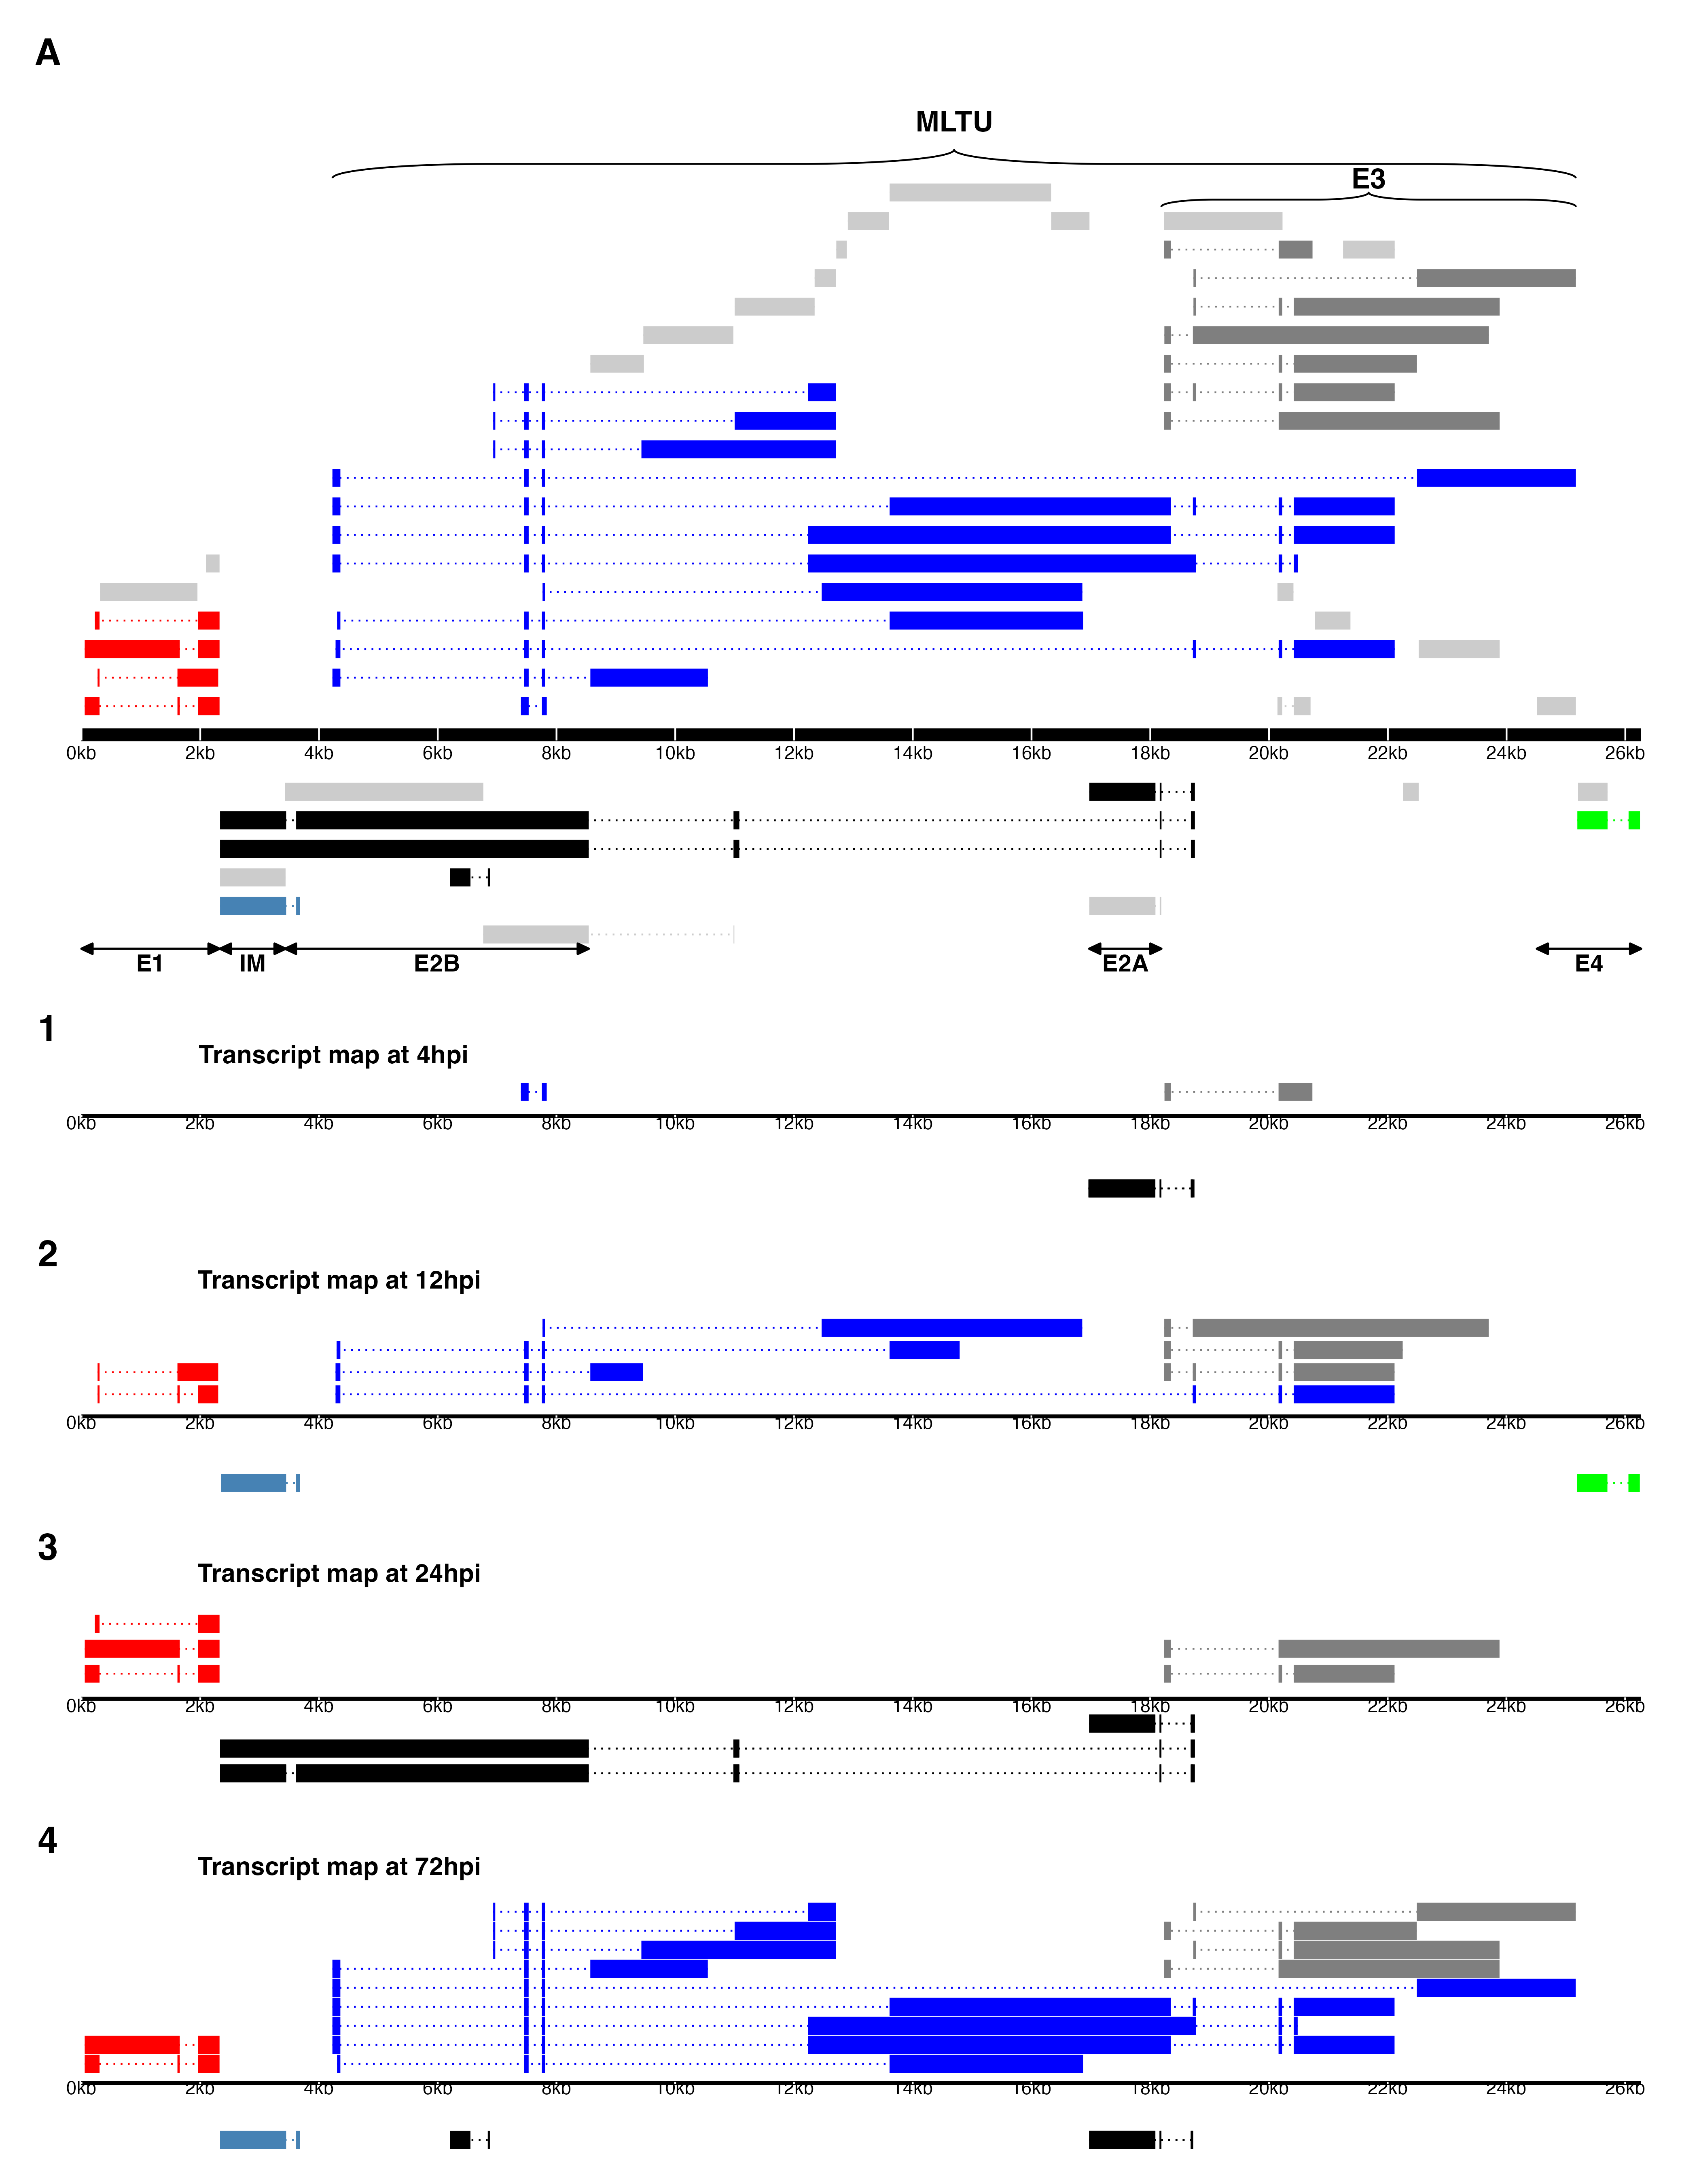
\includegraphics{results/r/figures/figure3.png}
\caption{\textbf{Figure 3. A) Transcriptome of THEV from RNA-seq.} THEV
transcripts assembled from all time points by StringTie are unified
forming this final transcriptome (splicing map). Transcripts belonging
to the same transcription unit (TU) are located in close proximity on
the genome and are color coded and labeled in this figure as such. The
organization of TUs in the THEV genome is unsurprisingly similar to
MAdVs; however, the MAdV genome shows significantly more transcripts.
The TUs are color coded: E1 transcripts - red, E2 - black, E3 - dark
grey, E4 - green, MLTU - blue. Predicted ORFs are also indicated here,
colored light grey. \textbf{B) THEV transcripts identified at given time
points.} Transcripts are color coded as explained in \textbf{(A)}.}
\end{figure}

\begin{figure}
\centering
\includegraphics{results/r/figures/figure_4a_d.png}
\caption{\textbf{Figure 4: Changes in splicing and expression profile of
THEV over time.} \textbf{A) Normalized (FPKM) expression levels of
transcripts over time.} The expression levels (FPKM) of individual
transcripts as a percentage of the total expression of all transcripts
at each time point are indicated. Only transcripts from our RNA-seq data
are included here. \textbf{B) Normalized (FPKM) expression levels of
transcripts by region over time.} The expression levels of each
region/TU as a percentage of the total expression of all transcripts at
each time point are indicated. Region expression levels were calculated
by summing up the FPKMs of all transcripts categorized in that region.
\textbf{C) Relative abundances of all splice junctions grouped by
region/TU over time.} After assigning all 2,457 unique junctions to a TU
and the total junction reads counted at each time point for each region,
the total junction reads for each TU were plotted as percentages of all
junction reads at each time point. Note that the junction read counts
are not normalized. \textbf{D) Relative abundances of junctions in
transcriptome grouped by region/TU over time.} This is identical to
\textbf{(C)}, except that only the junctions found in the full
transcriptome obtained from the RNA-seq data were included.}
\end{figure}

\begin{figure}
\centering
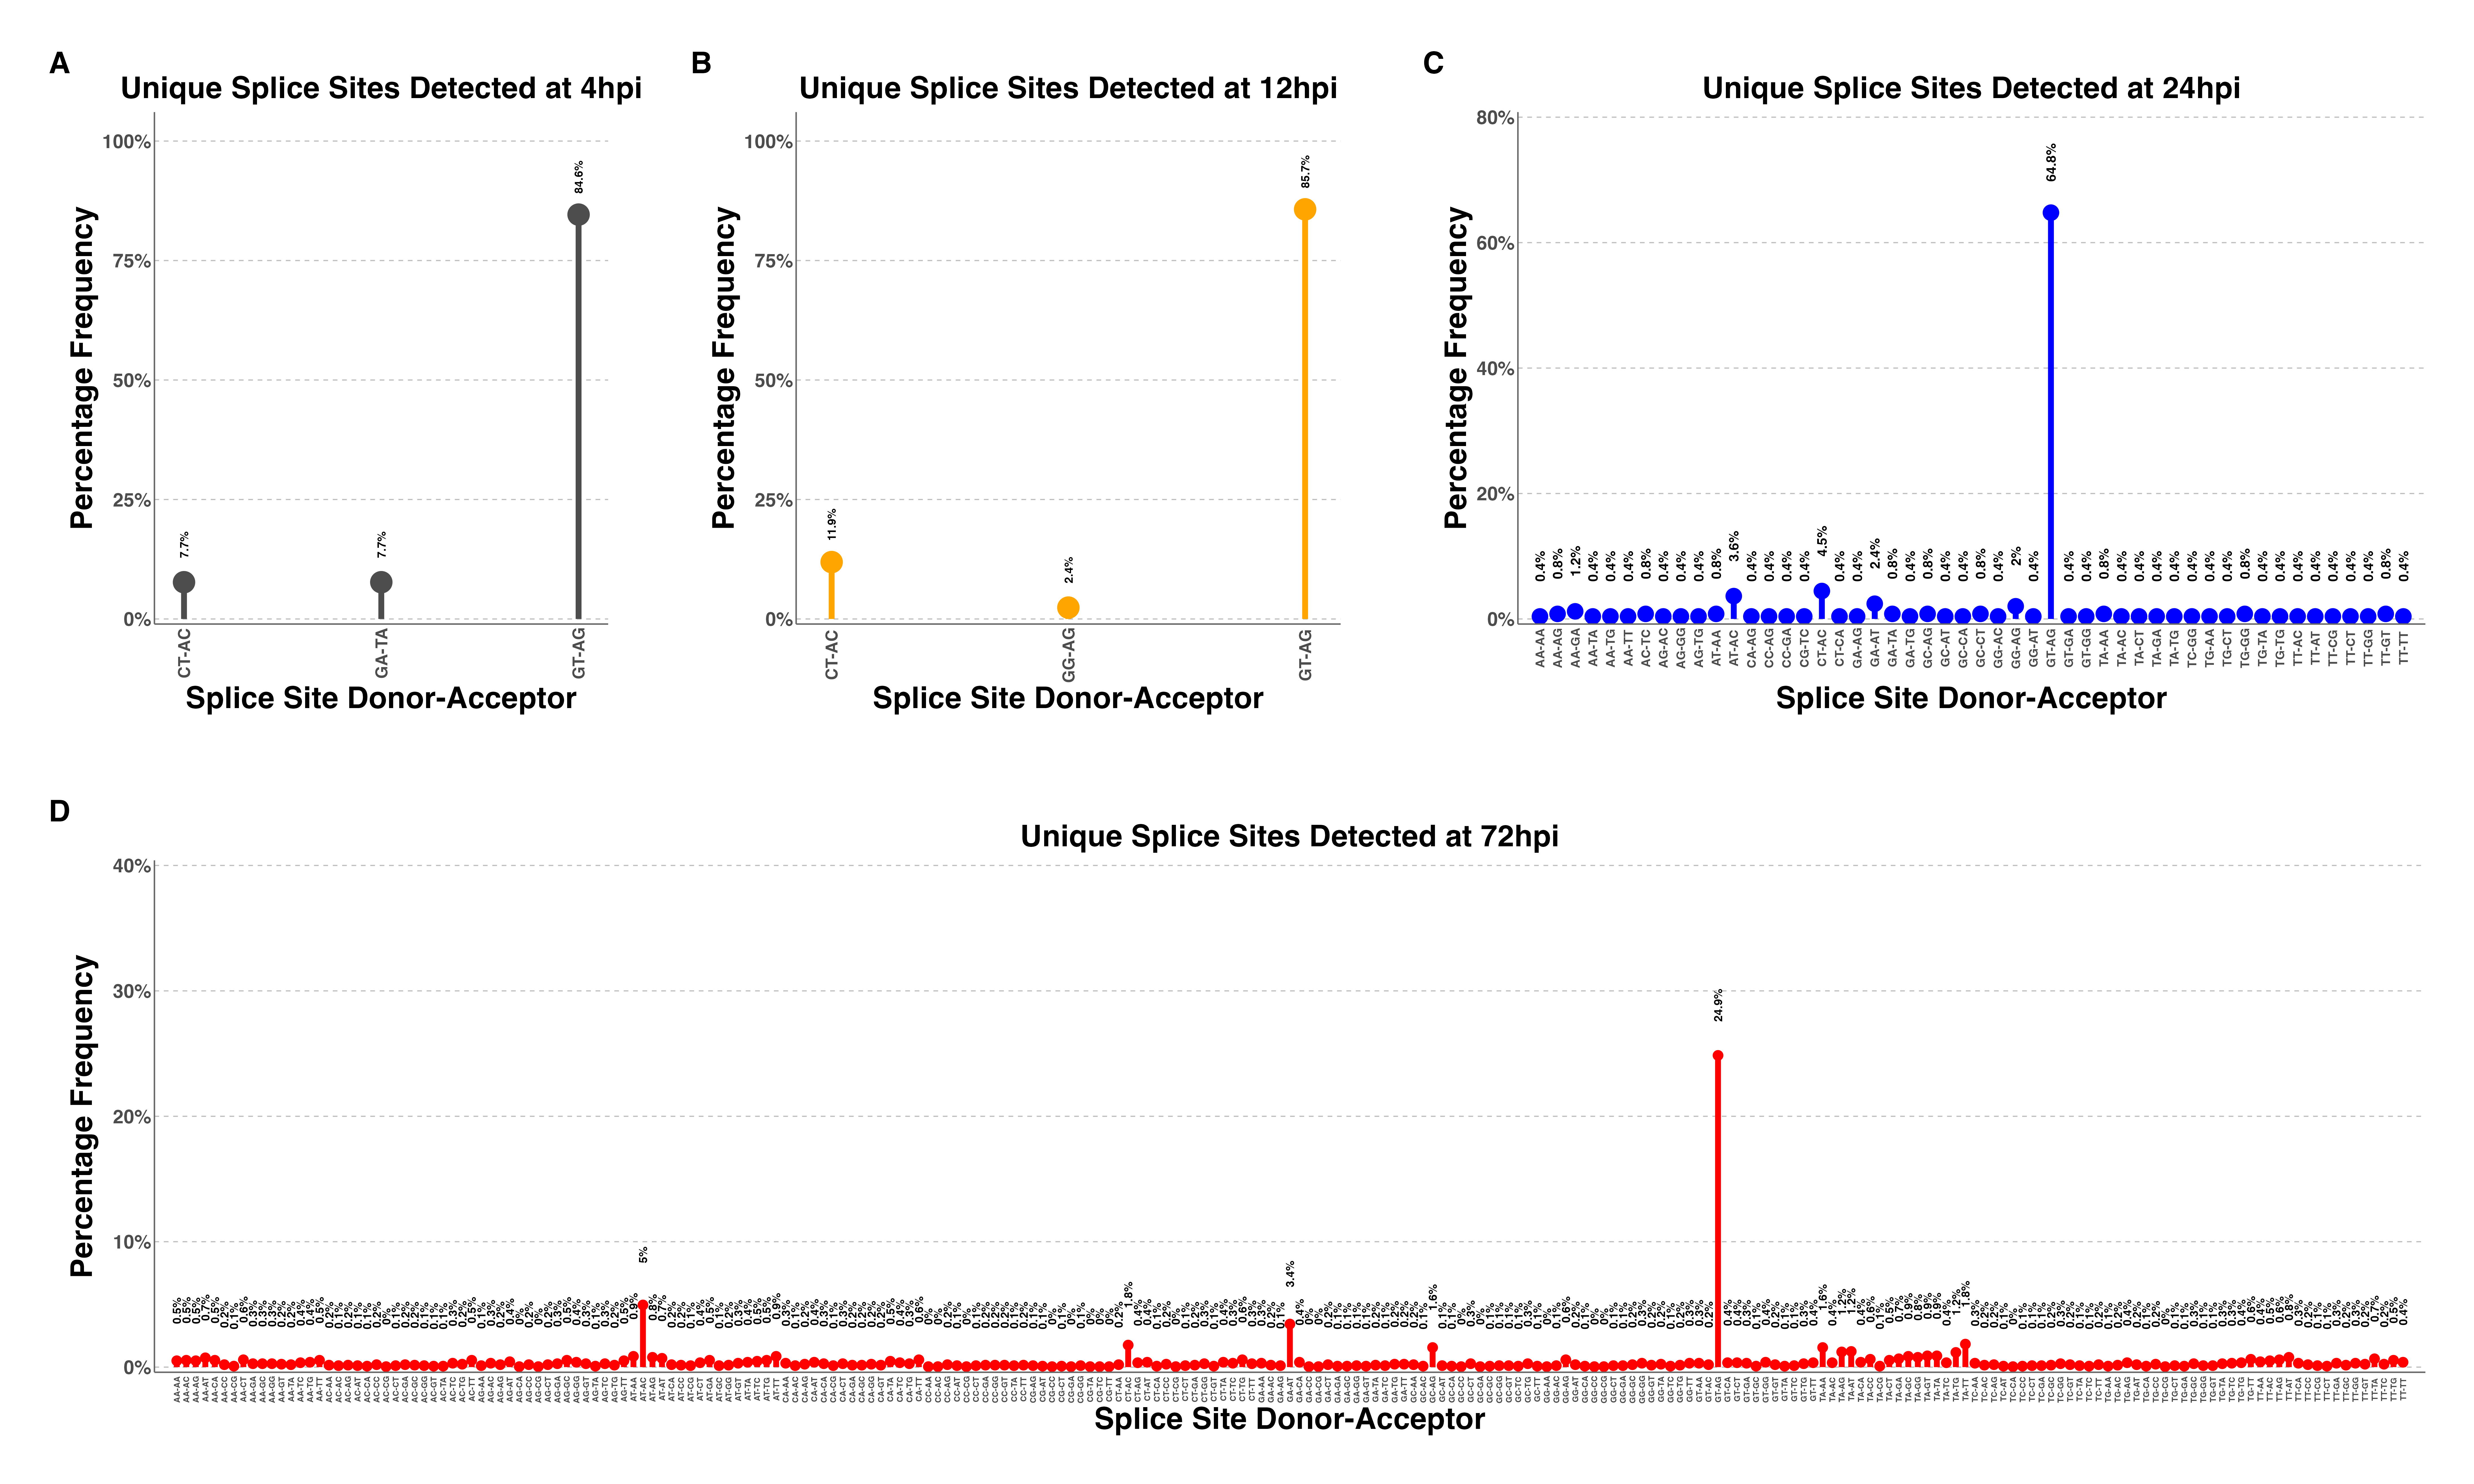
\includegraphics{results/r/figures/figure_5a_d.png}
\caption{\textbf{Figure 5: Changes in splice donor-acceptor nucleotides
over time.} The splice donor-acceptor nucleotides of THEV just like
other AdVs is mostly the canonical GU-AG. At early time points (4h.p.i
and 12h.p.i \textbf{(A)} and \textbf{(B)}, respectively) the junction
nucleotides used appear to be well scrutinized or restricted, utilizing
mostly the canonical splice nucleotides. However, as the infection
progresses to the late stages (24h.p.i and 72h.p.i \textbf{(C)} and
\textbf{(D)}, respectively), the selectivity of specific splice
acceptor-donor pairs seems to degenerate significantly, such that all
combinations of nucleotides are utilized.}
\end{figure}

\begin{figure}
\centering
\includegraphics{results/r/figures/figure_6.png}
\caption{\textbf{Figure 6: The splice map of the E1 transcription unit
(TU).} Exons are depicted as boxes connected by introns (dotted lines).
Transcripts from RNA-seq data are colored red, predicted ORFs are
colored grey, and transcripts or ORFs discovered by other means are
colored black. Each transcript or ORF is labelled with its name to the
right. The start codon (SC) and stop codon (STC) of the 5'-most CDS of
each transcript is indicated with the nucleotide position in brackets.
The region of the virus is depicted at the bottom as a black line with
labels of the nucleotide positions for reference. The table shows
sequence reads covering the splice junctions with information about
their validation status using cloning and Sanger sequencing.}
\end{figure}

\begin{figure}
\centering
\includegraphics{results/r/figures/figure_7.png}
\caption{\textbf{Figure 7: The splice map of the E2 and IM TUs.} Exons
are depicted as boxes connected by introns (dotted lines). Red
transcripts are generated from RNA-seq data and predicted ORFs are
colored grey. TRXPT\_21B discovered by 3'RACE is colored black. Each
transcript or ORF is labelled with its name to the right. The SC and STC
of the 5'-most CDS of each transcript are indicated with the nucleotide
position in brackets. The region of the virus is depicted at the bottom
as a black line with labels of the nucleotide positions for reference.
The table shows sequence reads covering the splice junctions with
information about their validation status using cloning and Sanger
sequencing.}
\end{figure}

\begin{figure}
\centering
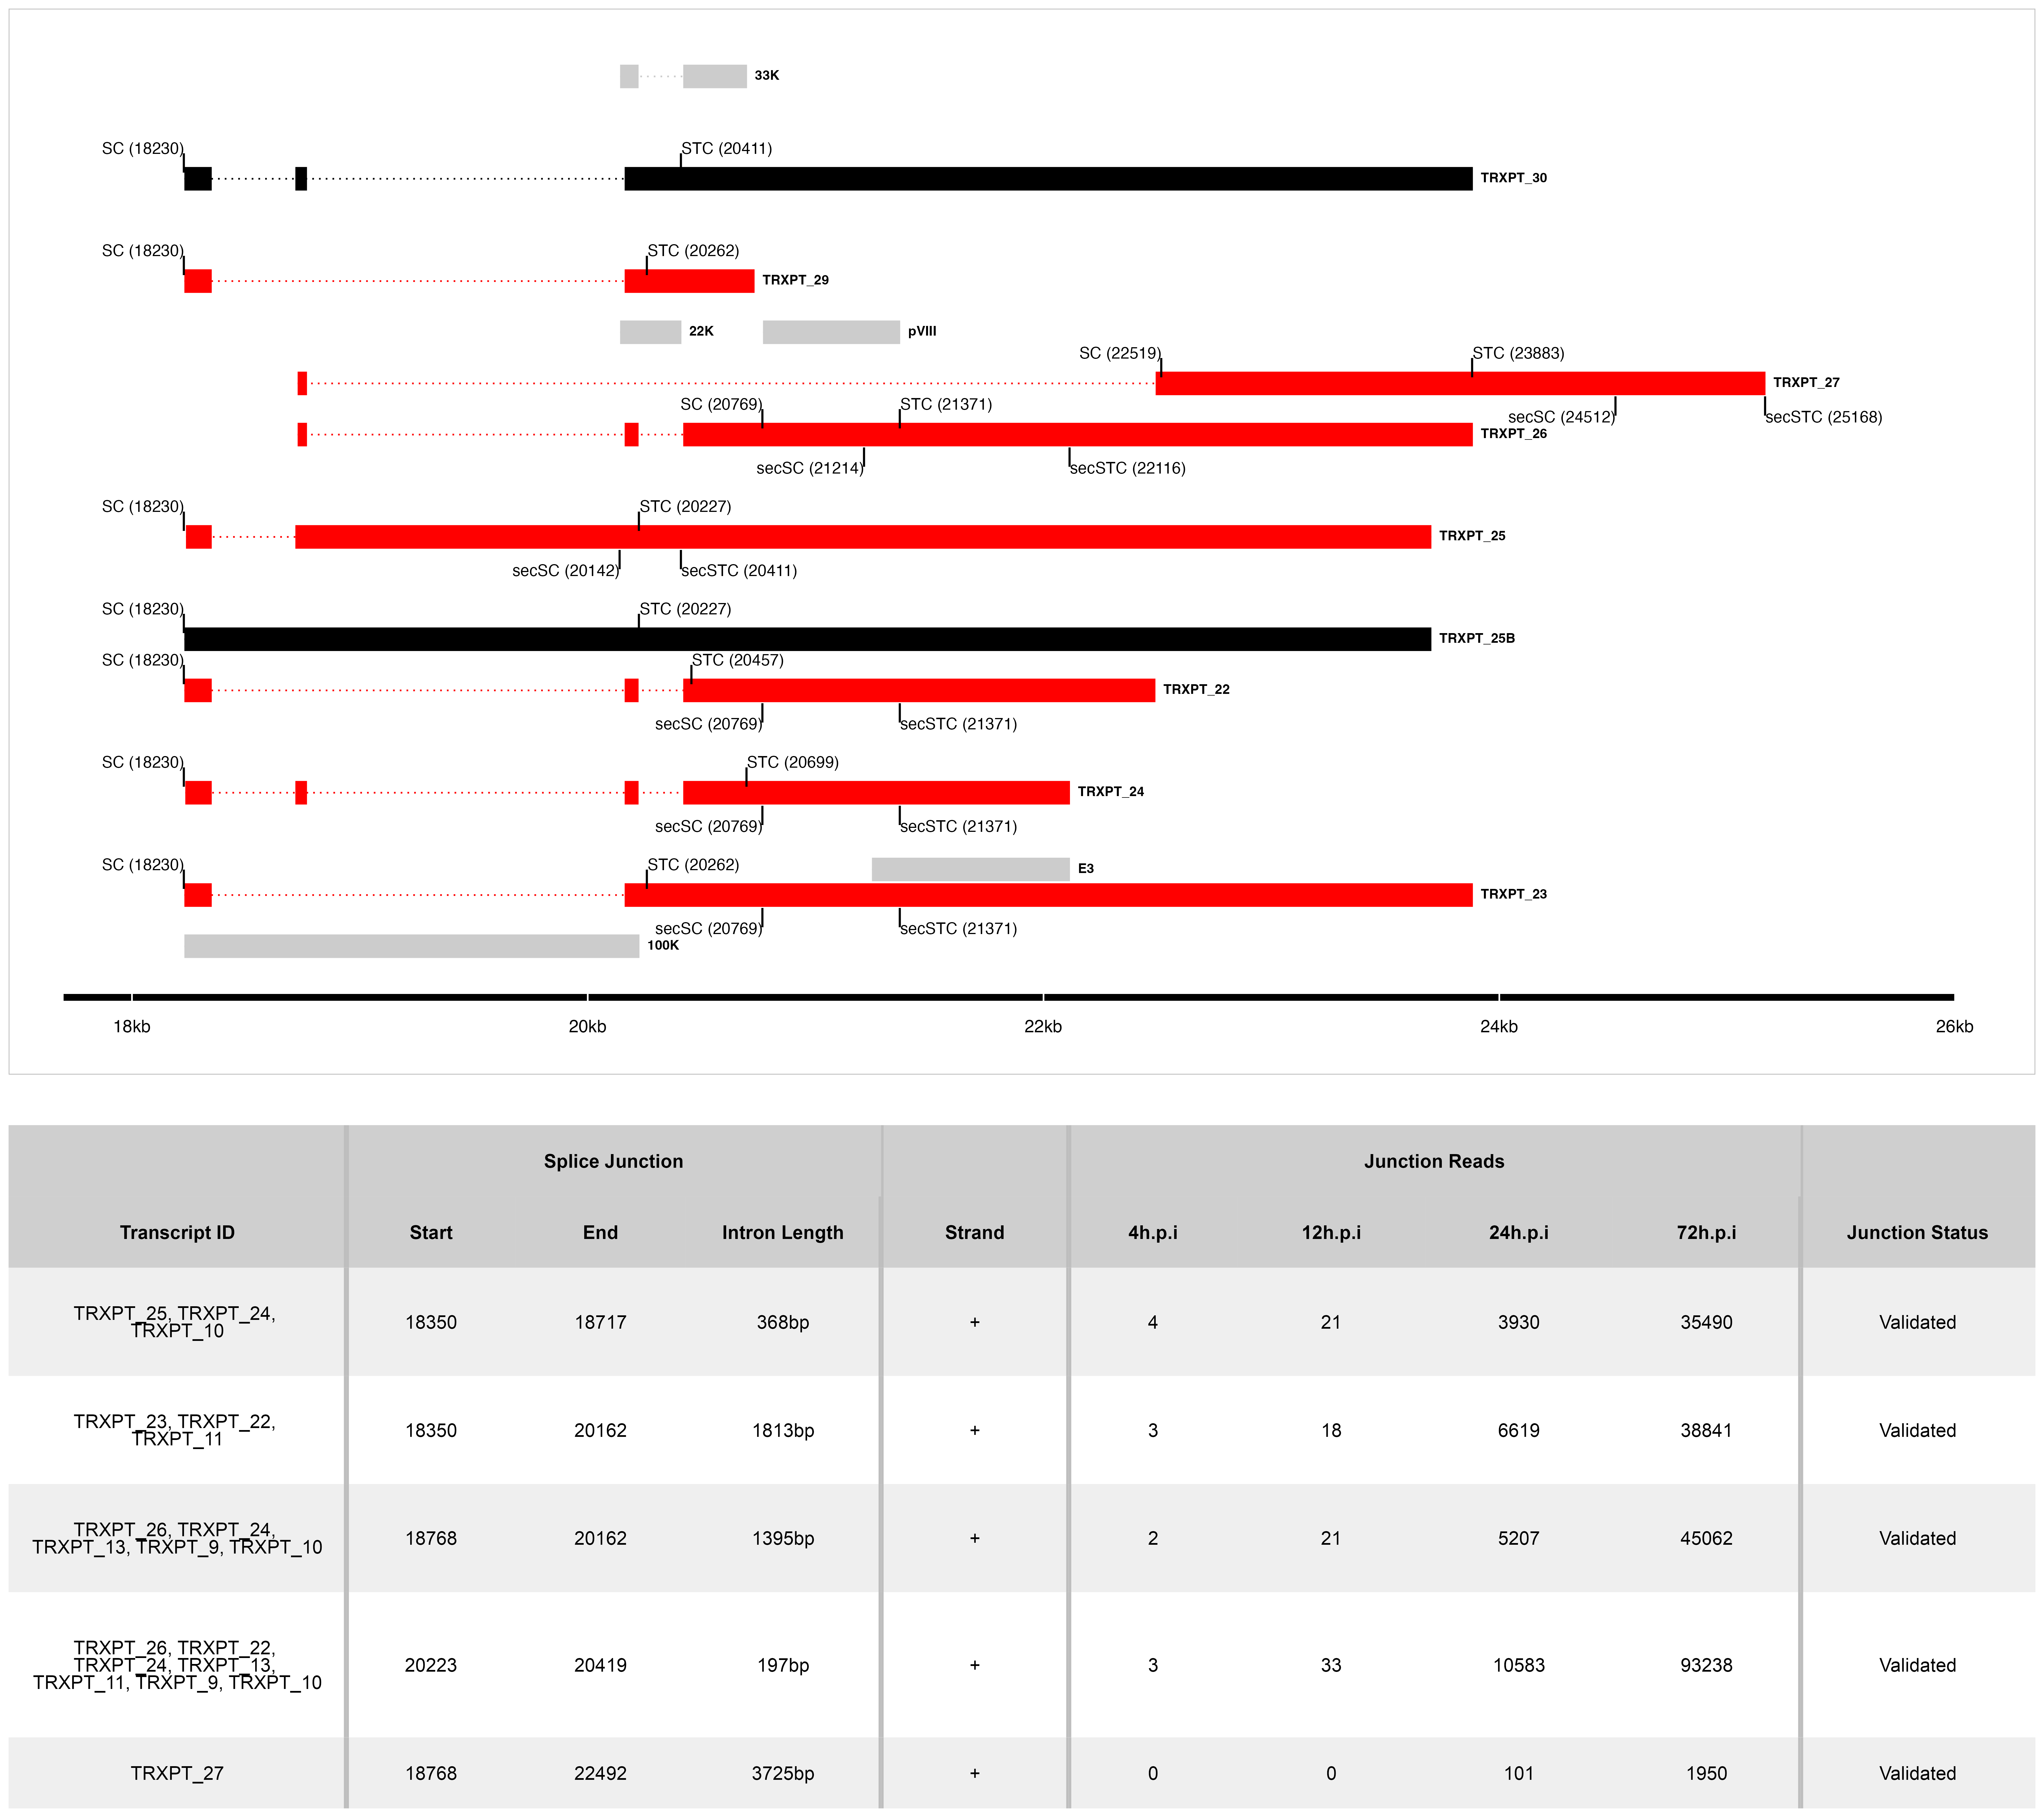
\includegraphics{results/r/figures/figure_8.png}
\caption{\textbf{Figure 8: The splice map of the E3 TU.} Exons are
depicted as boxes connected by introns (dotted lines). Red transcripts
are generated from RNA-seq data and predicted ORFs are colored grey.
Transcripts discovered by other means are colored black. Each transcript
or ORF is labelled with its name to the right. The start codon (SC) and
stop codon (STC) of the 5'-most CDS of each transcript are indicated
with the nucleotide position in brackets. Similarly, the secondary SC
(secSC) and secondary STC (secSTC) are shown. The region of the virus is
depicted at the bottom as a black line with labels of the nucleotide
positions for reference. The table shows sequence reads covering the
splice junctions with information about their validation status using
cloning and Sanger sequencing.}
\end{figure}

\begin{figure}
\centering
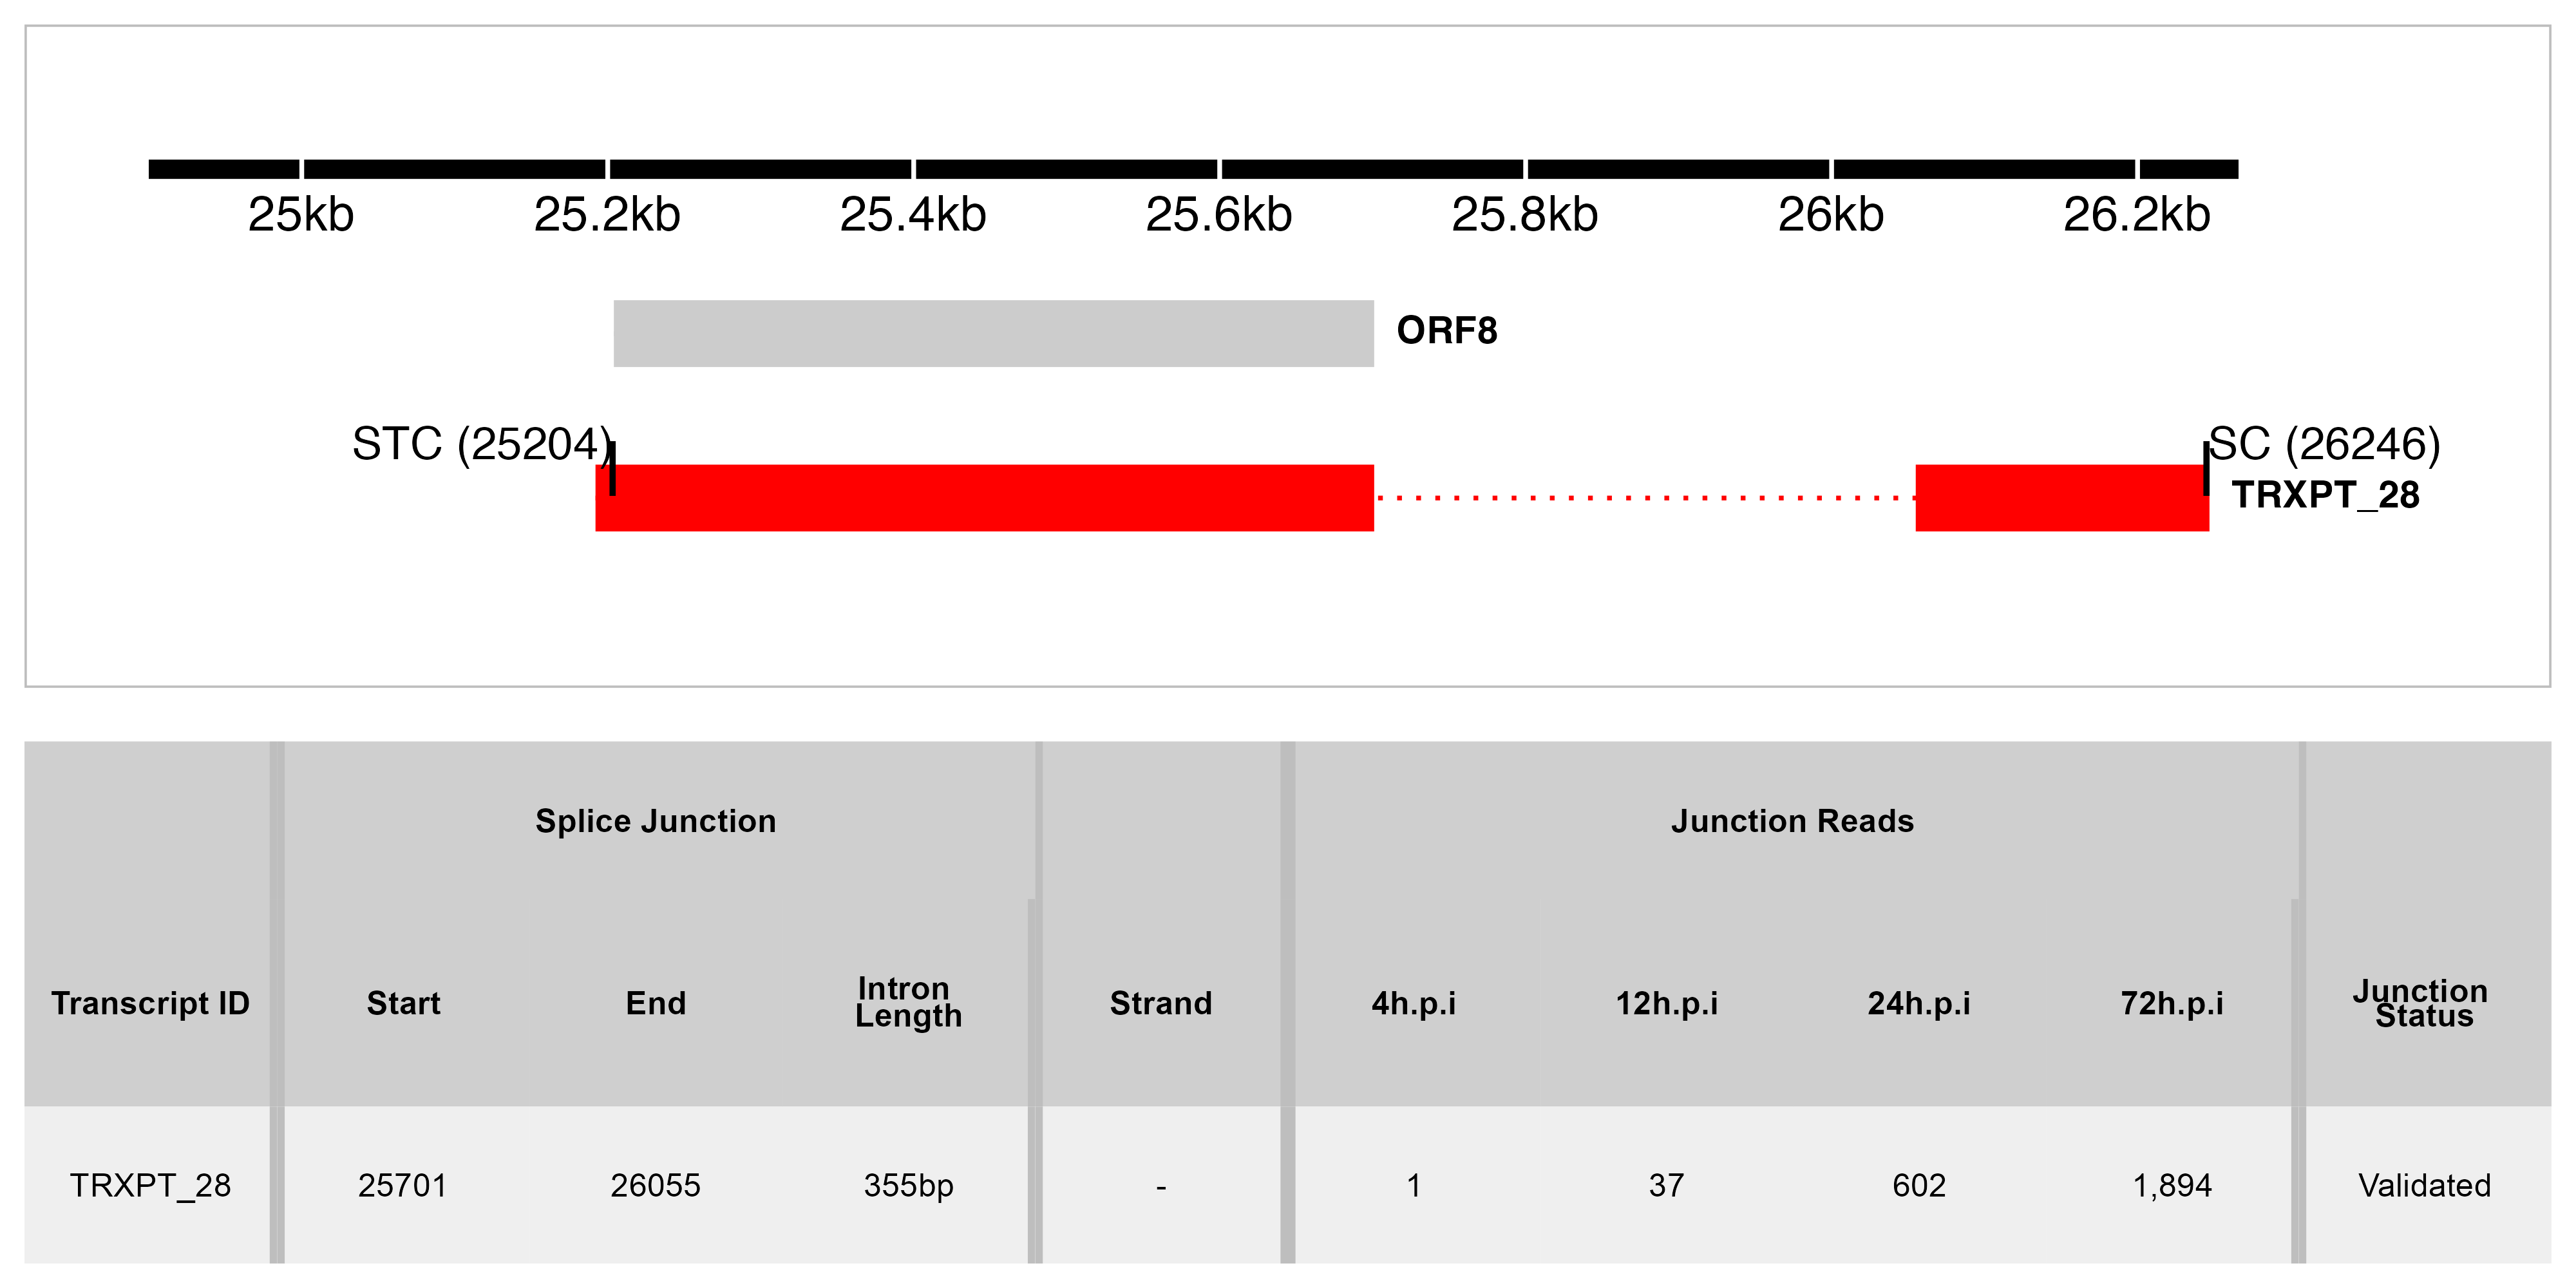
\includegraphics{results/r/figures/figure_9.png}
\caption{\textbf{Figure 9: The splice map of the E4 TU.} Exons are
depicted as boxes connected by introns (dotted lines). The transcript
from RNA-seq data is colored red and the predicted ORF, grey. The
transcript and ORF are labelled with their names to the right. The start
codon (SC) and stop codon (STC) of the 5'-most CDS are indicated with
the nucleotide position in brackets. The region of the virus is depicted
at the bottom as a black line with labels of the nucleotide positions
for reference. The table shows sequence reads covering the splice
junction with its validation status using cloning and Sanger
sequencing.}
\end{figure}

\newpage

\begin{figure}
\centering
\includegraphics{results/r/figures/figure_10.png}
\caption{\textbf{Figure 10: The splice map of the MLTU.} Exons are
depicted as boxes connected by introns (dotted lines). The transcripts
from our RNA-seq data are colored red and the predicted ORFs, grey. The
transcripts and ORFs are labelled with their names to the right. The
start codon (SC) and stop codon (STC) of the 5'-most CDS of each
transcript is indicated with the nucleotide position in brackets.
Similarly, the secondary SC (secSC) and secondary STC (secSTC) are
shown. The region of the virus is depicted at the bottom as a black line
with labels of the nucleotide positions for reference. The table shows
sequence reads covering the splice junctions with information about
their validation status using cloning and Sanger sequencing.}
\end{figure}

\newpage

\FloatBarrier

\global\setlength{\Oldarrayrulewidth}{\arrayrulewidth}

\global\setlength{\Oldtabcolsep}{\tabcolsep}

\setlength{\tabcolsep}{2pt}

\renewcommand*{\arraystretch}{1.5}



\providecommand{\ascline}[3]{\noalign{\global\arrayrulewidth #1}\arrayrulecolor[HTML]{#2}\cline{#3}}

\begin{longtable}[l]{|p{1.50in}|p{0.75in}|p{0.75in}|p{0.75in}|p{0.75in}|p{0.75in}}

\caption{Table\ 1:\ Overview\ of\ sequencing\ results}\\

\hhline{>{\arrayrulecolor[HTML]{000000}\global\arrayrulewidth=0pt}->{\arrayrulecolor[HTML]{000000}\global\arrayrulewidth=0pt}->{\arrayrulecolor[HTML]{000000}\global\arrayrulewidth=0pt}->{\arrayrulecolor[HTML]{000000}\global\arrayrulewidth=0pt}->{\arrayrulecolor[HTML]{000000}\global\arrayrulewidth=0pt}->{\arrayrulecolor[HTML]{000000}\global\arrayrulewidth=0pt}-}

\multicolumn{1}{>{\cellcolor[HTML]{CFCFCF}\raggedright}m{\dimexpr 1.5in+0\tabcolsep}}{\textcolor[HTML]{000000}{\fontsize{8}{8}\selectfont{\textbf{Metric}}}} & \multicolumn{1}{>{\cellcolor[HTML]{CFCFCF}\raggedright}m{\dimexpr 0.75in+0\tabcolsep}}{\textcolor[HTML]{000000}{\fontsize{8}{8}\selectfont{\textbf{4h.p.i}}}} & \multicolumn{1}{>{\cellcolor[HTML]{CFCFCF}\raggedright}m{\dimexpr 0.75in+0\tabcolsep}}{\textcolor[HTML]{000000}{\fontsize{8}{8}\selectfont{\textbf{12h.p.i}}}} & \multicolumn{1}{>{\cellcolor[HTML]{CFCFCF}\raggedright}m{\dimexpr 0.75in+0\tabcolsep}}{\textcolor[HTML]{000000}{\fontsize{8}{8}\selectfont{\textbf{24h.p.i}}}} & \multicolumn{1}{>{\cellcolor[HTML]{CFCFCF}\raggedright}m{\dimexpr 0.75in+0\tabcolsep}}{\textcolor[HTML]{000000}{\fontsize{8}{8}\selectfont{\textbf{72h.p.i}}}} & \multicolumn{1}{>{\cellcolor[HTML]{CFCFCF}\raggedright}m{\dimexpr 0.75in+0\tabcolsep}}{\textcolor[HTML]{000000}{\fontsize{8}{8}\selectfont{\textbf{Total}}}} \\

\noalign{\global\arrayrulewidth 0pt}\arrayrulecolor[HTML]{000000}

\endfirsthead

\hhline{>{\arrayrulecolor[HTML]{000000}\global\arrayrulewidth=0pt}->{\arrayrulecolor[HTML]{000000}\global\arrayrulewidth=0pt}->{\arrayrulecolor[HTML]{000000}\global\arrayrulewidth=0pt}->{\arrayrulecolor[HTML]{000000}\global\arrayrulewidth=0pt}->{\arrayrulecolor[HTML]{000000}\global\arrayrulewidth=0pt}->{\arrayrulecolor[HTML]{000000}\global\arrayrulewidth=0pt}-}

\multicolumn{1}{>{\cellcolor[HTML]{CFCFCF}\raggedright}m{\dimexpr 1.5in+0\tabcolsep}}{\textcolor[HTML]{000000}{\fontsize{8}{8}\selectfont{\textbf{Metric}}}} & \multicolumn{1}{>{\cellcolor[HTML]{CFCFCF}\raggedright}m{\dimexpr 0.75in+0\tabcolsep}}{\textcolor[HTML]{000000}{\fontsize{8}{8}\selectfont{\textbf{4h.p.i}}}} & \multicolumn{1}{>{\cellcolor[HTML]{CFCFCF}\raggedright}m{\dimexpr 0.75in+0\tabcolsep}}{\textcolor[HTML]{000000}{\fontsize{8}{8}\selectfont{\textbf{12h.p.i}}}} & \multicolumn{1}{>{\cellcolor[HTML]{CFCFCF}\raggedright}m{\dimexpr 0.75in+0\tabcolsep}}{\textcolor[HTML]{000000}{\fontsize{8}{8}\selectfont{\textbf{24h.p.i}}}} & \multicolumn{1}{>{\cellcolor[HTML]{CFCFCF}\raggedright}m{\dimexpr 0.75in+0\tabcolsep}}{\textcolor[HTML]{000000}{\fontsize{8}{8}\selectfont{\textbf{72h.p.i}}}} & \multicolumn{1}{>{\cellcolor[HTML]{CFCFCF}\raggedright}m{\dimexpr 0.75in+0\tabcolsep}}{\textcolor[HTML]{000000}{\fontsize{8}{8}\selectfont{\textbf{Total}}}} \\

\noalign{\global\arrayrulewidth 0pt}\arrayrulecolor[HTML]{000000}

\endhead



\multicolumn{1}{>{\cellcolor[HTML]{EFEFEF}\raggedright}m{\dimexpr 1.5in+0\tabcolsep}}{\textcolor[HTML]{000000}{\fontsize{8}{8}\selectfont{\textbf{Total\ reads}}}} & \multicolumn{1}{>{\cellcolor[HTML]{EFEFEF}\raggedright}m{\dimexpr 0.75in+0\tabcolsep}}{\textcolor[HTML]{000000}{\fontsize{8}{8}\selectfont{1.17e+08}}} & \multicolumn{1}{>{\cellcolor[HTML]{EFEFEF}\raggedright}m{\dimexpr 0.75in+0\tabcolsep}}{\textcolor[HTML]{000000}{\fontsize{8}{8}\selectfont{7.63e+07}}} & \multicolumn{1}{>{\cellcolor[HTML]{EFEFEF}\raggedright}m{\dimexpr 0.75in+0\tabcolsep}}{\textcolor[HTML]{000000}{\fontsize{8}{8}\selectfont{1.20e+08}}} & \multicolumn{1}{>{\cellcolor[HTML]{EFEFEF}\raggedright}m{\dimexpr 0.75in+0\tabcolsep}}{\textcolor[HTML]{000000}{\fontsize{8}{8}\selectfont{1.15e+08}}} & \multicolumn{1}{>{\cellcolor[HTML]{EFEFEF}\raggedright}m{\dimexpr 0.75in+0\tabcolsep}}{\textcolor[HTML]{000000}{\fontsize{8}{8}\selectfont{4.28e+08}}} \\

\noalign{\global\arrayrulewidth 0pt}\arrayrulecolor[HTML]{000000}





\multicolumn{1}{>{\raggedright}m{\dimexpr 1.5in+0\tabcolsep}}{\textcolor[HTML]{000000}{\fontsize{8}{8}\selectfont{\textbf{Mapped\ }}}\textcolor[HTML]{000000}{\fontsize{8}{8}\selectfont{\textbf{\linebreak }}}\textcolor[HTML]{000000}{\fontsize{8}{8}\selectfont{\textbf{\ (Host)}}}} & \multicolumn{1}{>{\raggedright}m{\dimexpr 0.75in+0\tabcolsep}}{\textcolor[HTML]{000000}{\fontsize{8}{8}\selectfont{1.04e+08\ }}\textcolor[HTML]{000000}{\fontsize{8}{8}\selectfont{\linebreak }}\textcolor[HTML]{000000}{\fontsize{8}{8}\selectfont{(89.06\%)}}} & \multicolumn{1}{>{\raggedright}m{\dimexpr 0.75in+0\tabcolsep}}{\textcolor[HTML]{000000}{\fontsize{8}{8}\selectfont{6.79e+07\ }}\textcolor[HTML]{000000}{\fontsize{8}{8}\selectfont{\linebreak }}\textcolor[HTML]{000000}{\fontsize{8}{8}\selectfont{(89.0393\%)}}} & \multicolumn{1}{>{\raggedright}m{\dimexpr 0.75in+0\tabcolsep}}{\textcolor[HTML]{000000}{\fontsize{8}{8}\selectfont{1.06e+08\ }}\textcolor[HTML]{000000}{\fontsize{8}{8}\selectfont{\linebreak }}\textcolor[HTML]{000000}{\fontsize{8}{8}\selectfont{(88.2719\%)}}} & \multicolumn{1}{>{\raggedright}m{\dimexpr 0.75in+0\tabcolsep}}{\textcolor[HTML]{000000}{\fontsize{8}{8}\selectfont{8.38e+07\ }}\textcolor[HTML]{000000}{\fontsize{8}{8}\selectfont{\linebreak }}\textcolor[HTML]{000000}{\fontsize{8}{8}\selectfont{(72.9802\%)}}} & \multicolumn{1}{>{\raggedright}m{\dimexpr 0.75in+0\tabcolsep}}{\textcolor[HTML]{000000}{\fontsize{8}{8}\selectfont{3.62e+08}}} \\

\noalign{\global\arrayrulewidth 0pt}\arrayrulecolor[HTML]{000000}





\multicolumn{1}{>{\cellcolor[HTML]{EFEFEF}\raggedright}m{\dimexpr 1.5in+0\tabcolsep}}{\textcolor[HTML]{000000}{\fontsize{8}{8}\selectfont{\textbf{Mapped\ }}}\textcolor[HTML]{000000}{\fontsize{8}{8}\selectfont{\textbf{\linebreak }}}\textcolor[HTML]{000000}{\fontsize{8}{8}\selectfont{\textbf{\ (THEV)}}}} & \multicolumn{1}{>{\cellcolor[HTML]{EFEFEF}\raggedright}m{\dimexpr 0.75in+0\tabcolsep}}{\textcolor[HTML]{000000}{\fontsize{8}{8}\selectfont{4.32e+02\ }}\textcolor[HTML]{000000}{\fontsize{8}{8}\selectfont{\linebreak }}\textcolor[HTML]{000000}{\fontsize{8}{8}\selectfont{(\ 0.0004\%)}}} & \multicolumn{1}{>{\cellcolor[HTML]{EFEFEF}\raggedright}m{\dimexpr 0.75in+0\tabcolsep}}{\textcolor[HTML]{000000}{\fontsize{8}{8}\selectfont{6.70e+03\ }}\textcolor[HTML]{000000}{\fontsize{8}{8}\selectfont{\linebreak }}\textcolor[HTML]{000000}{\fontsize{8}{8}\selectfont{(\ 0.0088\%)}}} & \multicolumn{1}{>{\cellcolor[HTML]{EFEFEF}\raggedright}m{\dimexpr 0.75in+0\tabcolsep}}{\textcolor[HTML]{000000}{\fontsize{8}{8}\selectfont{1.18e+06\ }}\textcolor[HTML]{000000}{\fontsize{8}{8}\selectfont{\linebreak }}\textcolor[HTML]{000000}{\fontsize{8}{8}\selectfont{(\ 0.9841\%)}}} & \multicolumn{1}{>{\cellcolor[HTML]{EFEFEF}\raggedright}m{\dimexpr 0.75in+0\tabcolsep}}{\textcolor[HTML]{000000}{\fontsize{8}{8}\selectfont{1.69e+07\ }}\textcolor[HTML]{000000}{\fontsize{8}{8}\selectfont{\linebreak }}\textcolor[HTML]{000000}{\fontsize{8}{8}\selectfont{(14.6904\%)}}} & \multicolumn{1}{>{\cellcolor[HTML]{EFEFEF}\raggedright}m{\dimexpr 0.75in+0\tabcolsep}}{\textcolor[HTML]{000000}{\fontsize{8}{8}\selectfont{1.81e+07}}} \\

\noalign{\global\arrayrulewidth 0pt}\arrayrulecolor[HTML]{000000}





\multicolumn{1}{>{\raggedright}m{\dimexpr 1.5in+0\tabcolsep}}{\textcolor[HTML]{000000}{\fontsize{8}{8}\selectfont{\textbf{Mean\ Per\ Base\ }}}\textcolor[HTML]{000000}{\fontsize{8}{8}\selectfont{\textbf{\linebreak }}}\textcolor[HTML]{000000}{\fontsize{8}{8}\selectfont{\textbf{\ Coverage/Depth}}}} & \multicolumn{1}{>{\raggedright}m{\dimexpr 0.75in+0\tabcolsep}}{\textcolor[HTML]{000000}{\fontsize{8}{8}\selectfont{2.42}}} & \multicolumn{1}{>{\raggedright}m{\dimexpr 0.75in+0\tabcolsep}}{\textcolor[HTML]{000000}{\fontsize{8}{8}\selectfont{37.71}}} & \multicolumn{1}{>{\raggedright}m{\dimexpr 0.75in+0\tabcolsep}}{\textcolor[HTML]{000000}{\fontsize{8}{8}\selectfont{\ 6,666.96}}} & \multicolumn{1}{>{\raggedright}m{\dimexpr 0.75in+0\tabcolsep}}{\textcolor[HTML]{000000}{\fontsize{8}{8}\selectfont{\ 95,041.7}}} & \multicolumn{1}{>{\raggedright}m{\dimexpr 0.75in+0\tabcolsep}}{\textcolor[HTML]{000000}{\fontsize{8}{8}\selectfont{101,749}}} \\

\noalign{\global\arrayrulewidth 0pt}\arrayrulecolor[HTML]{000000}





\multicolumn{1}{>{\cellcolor[HTML]{EFEFEF}\raggedright}m{\dimexpr 1.5in+0\tabcolsep}}{\textcolor[HTML]{000000}{\fontsize{8}{8}\selectfont{\textbf{Total\ unique\ }}}\textcolor[HTML]{000000}{\fontsize{8}{8}\selectfont{\textbf{\linebreak }}}\textcolor[HTML]{000000}{\fontsize{8}{8}\selectfont{\textbf{\ splice\ junctions}}}} & \multicolumn{1}{>{\cellcolor[HTML]{EFEFEF}\raggedright}m{\dimexpr 0.75in+0\tabcolsep}}{\textcolor[HTML]{000000}{\fontsize{8}{8}\selectfont{13}}} & \multicolumn{1}{>{\cellcolor[HTML]{EFEFEF}\raggedright}m{\dimexpr 0.75in+0\tabcolsep}}{\textcolor[HTML]{000000}{\fontsize{8}{8}\selectfont{37}}} & \multicolumn{1}{>{\cellcolor[HTML]{EFEFEF}\raggedright}m{\dimexpr 0.75in+0\tabcolsep}}{\textcolor[HTML]{000000}{\fontsize{8}{8}\selectfont{236}}} & \multicolumn{1}{>{\cellcolor[HTML]{EFEFEF}\raggedright}m{\dimexpr 0.75in+0\tabcolsep}}{\textcolor[HTML]{000000}{\fontsize{8}{8}\selectfont{2374}}} & \multicolumn{1}{>{\cellcolor[HTML]{EFEFEF}\raggedright}m{\dimexpr 0.75in+0\tabcolsep}}{\textcolor[HTML]{000000}{\fontsize{8}{8}\selectfont{2,457}}} \\

\noalign{\global\arrayrulewidth 0pt}\arrayrulecolor[HTML]{000000}





\multicolumn{1}{>{\raggedright}m{\dimexpr 1.5in+0\tabcolsep}}{\textcolor[HTML]{000000}{\fontsize{8}{8}\selectfont{\textbf{Junction\ coverage\ }}}\textcolor[HTML]{000000}{\fontsize{8}{8}\selectfont{\textbf{\linebreak }}}\textcolor[HTML]{000000}{\fontsize{8}{8}\selectfont{\textbf{\ Total\ (at\ least\ 1\ read)}}}} & \multicolumn{1}{>{\raggedright}m{\dimexpr 0.75in+0\tabcolsep}}{\textcolor[HTML]{000000}{\fontsize{8}{8}\selectfont{37}}} & \multicolumn{1}{>{\raggedright}m{\dimexpr 0.75in+0\tabcolsep}}{\textcolor[HTML]{000000}{\fontsize{8}{8}\selectfont{605}}} & \multicolumn{1}{>{\raggedright}m{\dimexpr 0.75in+0\tabcolsep}}{\textcolor[HTML]{000000}{\fontsize{8}{8}\selectfont{115075}}} & \multicolumn{1}{>{\raggedright}m{\dimexpr 0.75in+0\tabcolsep}}{\textcolor[HTML]{000000}{\fontsize{8}{8}\selectfont{2132806}}} & \multicolumn{1}{>{\raggedright}m{\dimexpr 0.75in+0\tabcolsep}}{\textcolor[HTML]{000000}{\fontsize{8}{8}\selectfont{2.25e+06}}} \\

\noalign{\global\arrayrulewidth 0pt}\arrayrulecolor[HTML]{000000}





\multicolumn{1}{>{\cellcolor[HTML]{EFEFEF}\raggedright}m{\dimexpr 1.5in+0\tabcolsep}}{\textcolor[HTML]{000000}{\fontsize{8}{8}\selectfont{\textbf{Junction\ coverage\ }}}\textcolor[HTML]{000000}{\fontsize{8}{8}\selectfont{\textbf{\linebreak }}}\textcolor[HTML]{000000}{\fontsize{8}{8}\selectfont{\textbf{\ Mean\ reads}}}} & \multicolumn{1}{>{\cellcolor[HTML]{EFEFEF}\raggedright}m{\dimexpr 0.75in+0\tabcolsep}}{\textcolor[HTML]{000000}{\fontsize{8}{8}\selectfont{2.8}}} & \multicolumn{1}{>{\cellcolor[HTML]{EFEFEF}\raggedright}m{\dimexpr 0.75in+0\tabcolsep}}{\textcolor[HTML]{000000}{\fontsize{8}{8}\selectfont{16.4}}} & \multicolumn{1}{>{\cellcolor[HTML]{EFEFEF}\raggedright}m{\dimexpr 0.75in+0\tabcolsep}}{\textcolor[HTML]{000000}{\fontsize{8}{8}\selectfont{487.6}}} & \multicolumn{1}{>{\cellcolor[HTML]{EFEFEF}\raggedright}m{\dimexpr 0.75in+0\tabcolsep}}{\textcolor[HTML]{000000}{\fontsize{8}{8}\selectfont{898.4}}} & \multicolumn{1}{>{\cellcolor[HTML]{EFEFEF}\raggedright}m{\dimexpr 0.75in+0\tabcolsep}}{\textcolor[HTML]{000000}{\fontsize{8}{8}\selectfont{351.3}}} \\

\noalign{\global\arrayrulewidth 0pt}\arrayrulecolor[HTML]{000000}





\multicolumn{1}{>{\raggedright}m{\dimexpr 1.5in+0\tabcolsep}}{\textcolor[HTML]{000000}{\fontsize{8}{8}\selectfont{\textbf{Junction\ coverage\ }}}\textcolor[HTML]{000000}{\fontsize{8}{8}\selectfont{\textbf{\linebreak }}}\textcolor[HTML]{000000}{\fontsize{8}{8}\selectfont{\textbf{\ (at\ least\ 10\ reads)}}}} & \multicolumn{1}{>{\raggedright}m{\dimexpr 0.75in+0\tabcolsep}}{\textcolor[HTML]{000000}{\fontsize{8}{8}\selectfont{0}}} & \multicolumn{1}{>{\raggedright}m{\dimexpr 0.75in+0\tabcolsep}}{\textcolor[HTML]{000000}{\fontsize{8}{8}\selectfont{13}}} & \multicolumn{1}{>{\raggedright}m{\dimexpr 0.75in+0\tabcolsep}}{\textcolor[HTML]{000000}{\fontsize{8}{8}\selectfont{132}}} & \multicolumn{1}{>{\raggedright}m{\dimexpr 0.75in+0\tabcolsep}}{\textcolor[HTML]{000000}{\fontsize{8}{8}\selectfont{1791}}} & \multicolumn{1}{>{\raggedright}m{\dimexpr 0.75in+0\tabcolsep}}{\textcolor[HTML]{000000}{\fontsize{8}{8}\selectfont{1,936}}} \\

\noalign{\global\arrayrulewidth 0pt}\arrayrulecolor[HTML]{000000}





\multicolumn{1}{>{\cellcolor[HTML]{EFEFEF}\raggedright}m{\dimexpr 1.5in+0\tabcolsep}}{\textcolor[HTML]{000000}{\fontsize{8}{8}\selectfont{\textbf{Junction\ coverage\ }}}\textcolor[HTML]{000000}{\fontsize{8}{8}\selectfont{\textbf{\linebreak }}}\textcolor[HTML]{000000}{\fontsize{8}{8}\selectfont{\textbf{\ (at\ least\ 100\ reads)}}}} & \multicolumn{1}{>{\cellcolor[HTML]{EFEFEF}\raggedright}m{\dimexpr 0.75in+0\tabcolsep}}{\textcolor[HTML]{000000}{\fontsize{8}{8}\selectfont{0}}} & \multicolumn{1}{>{\cellcolor[HTML]{EFEFEF}\raggedright}m{\dimexpr 0.75in+0\tabcolsep}}{\textcolor[HTML]{000000}{\fontsize{8}{8}\selectfont{1}}} & \multicolumn{1}{>{\cellcolor[HTML]{EFEFEF}\raggedright}m{\dimexpr 0.75in+0\tabcolsep}}{\textcolor[HTML]{000000}{\fontsize{8}{8}\selectfont{53}}} & \multicolumn{1}{>{\cellcolor[HTML]{EFEFEF}\raggedright}m{\dimexpr 0.75in+0\tabcolsep}}{\textcolor[HTML]{000000}{\fontsize{8}{8}\selectfont{805}}} & \multicolumn{1}{>{\cellcolor[HTML]{EFEFEF}\raggedright}m{\dimexpr 0.75in+0\tabcolsep}}{\textcolor[HTML]{000000}{\fontsize{8}{8}\selectfont{859}}} \\

\noalign{\global\arrayrulewidth 0pt}\arrayrulecolor[HTML]{000000}





\multicolumn{1}{>{\raggedright}m{\dimexpr 1.5in+0\tabcolsep}}{\textcolor[HTML]{000000}{\fontsize{8}{8}\selectfont{\textbf{Junction\ coverage\ }}}\textcolor[HTML]{000000}{\fontsize{8}{8}\selectfont{\textbf{\linebreak }}}\textcolor[HTML]{000000}{\fontsize{8}{8}\selectfont{\textbf{\ (at\ least\ 1000\ reads)}}}} & \multicolumn{1}{>{\raggedright}m{\dimexpr 0.75in+0\tabcolsep}}{\textcolor[HTML]{000000}{\fontsize{8}{8}\selectfont{0}}} & \multicolumn{1}{>{\raggedright}m{\dimexpr 0.75in+0\tabcolsep}}{\textcolor[HTML]{000000}{\fontsize{8}{8}\selectfont{0}}} & \multicolumn{1}{>{\raggedright}m{\dimexpr 0.75in+0\tabcolsep}}{\textcolor[HTML]{000000}{\fontsize{8}{8}\selectfont{18}}} & \multicolumn{1}{>{\raggedright}m{\dimexpr 0.75in+0\tabcolsep}}{\textcolor[HTML]{000000}{\fontsize{8}{8}\selectfont{168}}} & \multicolumn{1}{>{\raggedright}m{\dimexpr 0.75in+0\tabcolsep}}{\textcolor[HTML]{000000}{\fontsize{8}{8}\selectfont{186}}} \\

\noalign{\global\arrayrulewidth 0pt}\arrayrulecolor[HTML]{000000}





\end{longtable}



\arrayrulecolor[HTML]{000000}

\global\setlength{\arrayrulewidth}{\Oldarrayrulewidth}

\global\setlength{\tabcolsep}{\Oldtabcolsep}

\renewcommand*{\arraystretch}{1}

\FloatBarrier

\newpage

\global\setlength{\Oldarrayrulewidth}{\arrayrulewidth}

\global\setlength{\Oldtabcolsep}{\tabcolsep}

\setlength{\tabcolsep}{2pt}

\renewcommand*{\arraystretch}{1.5}



\providecommand{\ascline}[3]{\noalign{\global\arrayrulewidth #1}\arrayrulecolor[HTML]{#2}\cline{#3}}

\begin{longtable}[l]{|p{0.70in}|p{0.70in}|p{0.70in}|p{0.70in}|p{0.70in}|p{0.70in}|p{0.70in}|p{1.20in}}

\caption{Table\ 2a:\ Most\ abundant\ splice\ junctions\ at\ 12h.p.i}\\

\hhline{>{\arrayrulecolor[HTML]{000000}\global\arrayrulewidth=0pt}->{\arrayrulecolor[HTML]{000000}\global\arrayrulewidth=0pt}->{\arrayrulecolor[HTML]{000000}\global\arrayrulewidth=0pt}->{\arrayrulecolor[HTML]{000000}\global\arrayrulewidth=0pt}->{\arrayrulecolor[HTML]{000000}\global\arrayrulewidth=0pt}->{\arrayrulecolor[HTML]{000000}\global\arrayrulewidth=0pt}->{\arrayrulecolor[HTML]{000000}\global\arrayrulewidth=0pt}->{\arrayrulecolor[HTML]{000000}\global\arrayrulewidth=0pt}-}

\multicolumn{1}{>{\cellcolor[HTML]{CFCFCF}\centering}m{\dimexpr 0.7in+0\tabcolsep}}{\textcolor[HTML]{000000}{\fontsize{8}{8}\selectfont{\textbf{Timepoint}}}} & \multicolumn{1}{>{\cellcolor[HTML]{CFCFCF}\centering}m{\dimexpr 0.7in+0\tabcolsep}}{\textcolor[HTML]{000000}{\fontsize{8}{8}\selectfont{\textbf{Strand}}}} & \multicolumn{1}{>{\cellcolor[HTML]{CFCFCF}\centering}m{\dimexpr 0.7in+0\tabcolsep}}{\textcolor[HTML]{000000}{\fontsize{8}{8}\selectfont{\textbf{Start}}}} & \multicolumn{1}{>{\cellcolor[HTML]{CFCFCF}\centering}m{\dimexpr 0.7in+0\tabcolsep}}{\textcolor[HTML]{000000}{\fontsize{8}{8}\selectfont{\textbf{End}}}} & \multicolumn{1}{>{\cellcolor[HTML]{CFCFCF}\centering}m{\dimexpr 0.7in+0\tabcolsep}}{\textcolor[HTML]{000000}{\fontsize{8}{8}\selectfont{\textbf{Splice\_Site}}}} & \multicolumn{1}{>{\cellcolor[HTML]{CFCFCF}\centering}m{\dimexpr 0.7in+0\tabcolsep}}{\textcolor[HTML]{000000}{\fontsize{8}{8}\selectfont{\textbf{Region}}}} & \multicolumn{1}{>{\cellcolor[HTML]{CFCFCF}\centering}m{\dimexpr 0.7in+0\tabcolsep}}{\textcolor[HTML]{000000}{\fontsize{8}{8}\selectfont{\textbf{Intron\ Length}}}} & \multicolumn{1}{>{\cellcolor[HTML]{CFCFCF}\centering}m{\dimexpr 1.2in+0\tabcolsep}}{\textcolor[HTML]{000000}{\fontsize{8}{8}\selectfont{\textbf{Reads\ (Percentage)}}}} \\

\noalign{\global\arrayrulewidth 0pt}\arrayrulecolor[HTML]{000000}

\endfirsthead

\hhline{>{\arrayrulecolor[HTML]{000000}\global\arrayrulewidth=0pt}->{\arrayrulecolor[HTML]{000000}\global\arrayrulewidth=0pt}->{\arrayrulecolor[HTML]{000000}\global\arrayrulewidth=0pt}->{\arrayrulecolor[HTML]{000000}\global\arrayrulewidth=0pt}->{\arrayrulecolor[HTML]{000000}\global\arrayrulewidth=0pt}->{\arrayrulecolor[HTML]{000000}\global\arrayrulewidth=0pt}->{\arrayrulecolor[HTML]{000000}\global\arrayrulewidth=0pt}->{\arrayrulecolor[HTML]{000000}\global\arrayrulewidth=0pt}-}

\multicolumn{1}{>{\cellcolor[HTML]{CFCFCF}\centering}m{\dimexpr 0.7in+0\tabcolsep}}{\textcolor[HTML]{000000}{\fontsize{8}{8}\selectfont{\textbf{Timepoint}}}} & \multicolumn{1}{>{\cellcolor[HTML]{CFCFCF}\centering}m{\dimexpr 0.7in+0\tabcolsep}}{\textcolor[HTML]{000000}{\fontsize{8}{8}\selectfont{\textbf{Strand}}}} & \multicolumn{1}{>{\cellcolor[HTML]{CFCFCF}\centering}m{\dimexpr 0.7in+0\tabcolsep}}{\textcolor[HTML]{000000}{\fontsize{8}{8}\selectfont{\textbf{Start}}}} & \multicolumn{1}{>{\cellcolor[HTML]{CFCFCF}\centering}m{\dimexpr 0.7in+0\tabcolsep}}{\textcolor[HTML]{000000}{\fontsize{8}{8}\selectfont{\textbf{End}}}} & \multicolumn{1}{>{\cellcolor[HTML]{CFCFCF}\centering}m{\dimexpr 0.7in+0\tabcolsep}}{\textcolor[HTML]{000000}{\fontsize{8}{8}\selectfont{\textbf{Splice\_Site}}}} & \multicolumn{1}{>{\cellcolor[HTML]{CFCFCF}\centering}m{\dimexpr 0.7in+0\tabcolsep}}{\textcolor[HTML]{000000}{\fontsize{8}{8}\selectfont{\textbf{Region}}}} & \multicolumn{1}{>{\cellcolor[HTML]{CFCFCF}\centering}m{\dimexpr 0.7in+0\tabcolsep}}{\textcolor[HTML]{000000}{\fontsize{8}{8}\selectfont{\textbf{Intron\ Length}}}} & \multicolumn{1}{>{\cellcolor[HTML]{CFCFCF}\centering}m{\dimexpr 1.2in+0\tabcolsep}}{\textcolor[HTML]{000000}{\fontsize{8}{8}\selectfont{\textbf{Reads\ (Percentage)}}}} \\

\noalign{\global\arrayrulewidth 0pt}\arrayrulecolor[HTML]{000000}

\endhead



\multicolumn{1}{>{\cellcolor[HTML]{EFEFEF}\centering}m{\dimexpr 0.7in+0\tabcolsep}}{\textcolor[HTML]{000000}{\fontsize{8}{8}\selectfont{12hpi}}} & \multicolumn{1}{>{\cellcolor[HTML]{EFEFEF}\centering}m{\dimexpr 0.7in+0\tabcolsep}}{\textcolor[HTML]{000000}{\fontsize{8}{8}\selectfont{-}}} & \multicolumn{1}{>{\cellcolor[HTML]{EFEFEF}\centering}m{\dimexpr 0.7in+0\tabcolsep}}{\textcolor[HTML]{000000}{\fontsize{8}{8}\selectfont{18,087}}} & \multicolumn{1}{>{\cellcolor[HTML]{EFEFEF}\centering}m{\dimexpr 0.7in+0\tabcolsep}}{\textcolor[HTML]{000000}{\fontsize{8}{8}\selectfont{18,159}}} & \multicolumn{1}{>{\cellcolor[HTML]{EFEFEF}\centering}m{\dimexpr 0.7in+0\tabcolsep}}{\textcolor[HTML]{000000}{\fontsize{8}{8}\selectfont{GU-AG}}} & \multicolumn{1}{>{\cellcolor[HTML]{EFEFEF}\centering}m{\dimexpr 0.7in+0\tabcolsep}}{\textcolor[HTML]{000000}{\fontsize{8}{8}\selectfont{E2}}} & \multicolumn{1}{>{\cellcolor[HTML]{EFEFEF}\centering}m{\dimexpr 0.7in+0\tabcolsep}}{\textcolor[HTML]{000000}{\fontsize{8}{8}\selectfont{72\ bp}}} & \multicolumn{1}{>{\cellcolor[HTML]{EFEFEF}\centering}m{\dimexpr 1.2in+0\tabcolsep}}{\textcolor[HTML]{000000}{\fontsize{8}{8}\selectfont{103\ (17\%)}}} \\

\noalign{\global\arrayrulewidth 0pt}\arrayrulecolor[HTML]{000000}





\multicolumn{1}{>{\centering}m{\dimexpr 0.7in+0\tabcolsep}}{\textcolor[HTML]{000000}{\fontsize{8}{8}\selectfont{12hpi}}} & \multicolumn{1}{>{\centering}m{\dimexpr 0.7in+0\tabcolsep}}{\textcolor[HTML]{000000}{\fontsize{8}{8}\selectfont{+}}} & \multicolumn{1}{>{\centering}m{\dimexpr 0.7in+0\tabcolsep}}{\textcolor[HTML]{000000}{\fontsize{8}{8}\selectfont{18,189}}} & \multicolumn{1}{>{\centering}m{\dimexpr 0.7in+0\tabcolsep}}{\textcolor[HTML]{000000}{\fontsize{8}{8}\selectfont{18,684}}} & \multicolumn{1}{>{\centering}m{\dimexpr 0.7in+0\tabcolsep}}{\textcolor[HTML]{000000}{\fontsize{8}{8}\selectfont{CU-AC}}} & \multicolumn{1}{>{\centering}m{\dimexpr 0.7in+0\tabcolsep}}{\textcolor[HTML]{000000}{\fontsize{8}{8}\selectfont{MLP}}} & \multicolumn{1}{>{\centering}m{\dimexpr 0.7in+0\tabcolsep}}{\textcolor[HTML]{000000}{\fontsize{8}{8}\selectfont{495\ bp}}} & \multicolumn{1}{>{\centering}m{\dimexpr 1.2in+0\tabcolsep}}{\textcolor[HTML]{000000}{\fontsize{8}{8}\selectfont{97\ (16\%)}}} \\

\noalign{\global\arrayrulewidth 0pt}\arrayrulecolor[HTML]{000000}





\multicolumn{1}{>{\cellcolor[HTML]{EFEFEF}\centering}m{\dimexpr 0.7in+0\tabcolsep}}{\textcolor[HTML]{000000}{\fontsize{8}{8}\selectfont{12hpi}}} & \multicolumn{1}{>{\cellcolor[HTML]{EFEFEF}\centering}m{\dimexpr 0.7in+0\tabcolsep}}{\textcolor[HTML]{000000}{\fontsize{8}{8}\selectfont{+}}} & \multicolumn{1}{>{\cellcolor[HTML]{EFEFEF}\centering}m{\dimexpr 0.7in+0\tabcolsep}}{\textcolor[HTML]{000000}{\fontsize{8}{8}\selectfont{7,531}}} & \multicolumn{1}{>{\cellcolor[HTML]{EFEFEF}\centering}m{\dimexpr 0.7in+0\tabcolsep}}{\textcolor[HTML]{000000}{\fontsize{8}{8}\selectfont{7,754}}} & \multicolumn{1}{>{\cellcolor[HTML]{EFEFEF}\centering}m{\dimexpr 0.7in+0\tabcolsep}}{\textcolor[HTML]{000000}{\fontsize{8}{8}\selectfont{GU-AG}}} & \multicolumn{1}{>{\cellcolor[HTML]{EFEFEF}\centering}m{\dimexpr 0.7in+0\tabcolsep}}{\textcolor[HTML]{000000}{\fontsize{8}{8}\selectfont{MLP}}} & \multicolumn{1}{>{\cellcolor[HTML]{EFEFEF}\centering}m{\dimexpr 0.7in+0\tabcolsep}}{\textcolor[HTML]{000000}{\fontsize{8}{8}\selectfont{223\ bp}}} & \multicolumn{1}{>{\cellcolor[HTML]{EFEFEF}\centering}m{\dimexpr 1.2in+0\tabcolsep}}{\textcolor[HTML]{000000}{\fontsize{8}{8}\selectfont{58\ (9.6\%)}}} \\

\noalign{\global\arrayrulewidth 0pt}\arrayrulecolor[HTML]{000000}





\multicolumn{1}{>{\centering}m{\dimexpr 0.7in+0\tabcolsep}}{\textcolor[HTML]{000000}{\fontsize{8}{8}\selectfont{12hpi}}} & \multicolumn{1}{>{\centering}m{\dimexpr 0.7in+0\tabcolsep}}{\textcolor[HTML]{000000}{\fontsize{8}{8}\selectfont{-}}} & \multicolumn{1}{>{\centering}m{\dimexpr 0.7in+0\tabcolsep}}{\textcolor[HTML]{000000}{\fontsize{8}{8}\selectfont{25,701}}} & \multicolumn{1}{>{\centering}m{\dimexpr 0.7in+0\tabcolsep}}{\textcolor[HTML]{000000}{\fontsize{8}{8}\selectfont{26,055}}} & \multicolumn{1}{>{\centering}m{\dimexpr 0.7in+0\tabcolsep}}{\textcolor[HTML]{000000}{\fontsize{8}{8}\selectfont{GU-AG}}} & \multicolumn{1}{>{\centering}m{\dimexpr 0.7in+0\tabcolsep}}{\textcolor[HTML]{000000}{\fontsize{8}{8}\selectfont{E4}}} & \multicolumn{1}{>{\centering}m{\dimexpr 0.7in+0\tabcolsep}}{\textcolor[HTML]{000000}{\fontsize{8}{8}\selectfont{354\ bp}}} & \multicolumn{1}{>{\centering}m{\dimexpr 1.2in+0\tabcolsep}}{\textcolor[HTML]{000000}{\fontsize{8}{8}\selectfont{37\ (6.1\%)}}} \\

\noalign{\global\arrayrulewidth 0pt}\arrayrulecolor[HTML]{000000}





\multicolumn{1}{>{\cellcolor[HTML]{EFEFEF}\centering}m{\dimexpr 0.7in+0\tabcolsep}}{\textcolor[HTML]{000000}{\fontsize{8}{8}\selectfont{12hpi}}} & \multicolumn{1}{>{\cellcolor[HTML]{EFEFEF}\centering}m{\dimexpr 0.7in+0\tabcolsep}}{\textcolor[HTML]{000000}{\fontsize{8}{8}\selectfont{+}}} & \multicolumn{1}{>{\cellcolor[HTML]{EFEFEF}\centering}m{\dimexpr 0.7in+0\tabcolsep}}{\textcolor[HTML]{000000}{\fontsize{8}{8}\selectfont{20,223}}} & \multicolumn{1}{>{\cellcolor[HTML]{EFEFEF}\centering}m{\dimexpr 0.7in+0\tabcolsep}}{\textcolor[HTML]{000000}{\fontsize{8}{8}\selectfont{20,419}}} & \multicolumn{1}{>{\cellcolor[HTML]{EFEFEF}\centering}m{\dimexpr 0.7in+0\tabcolsep}}{\textcolor[HTML]{000000}{\fontsize{8}{8}\selectfont{GU-AG}}} & \multicolumn{1}{>{\cellcolor[HTML]{EFEFEF}\centering}m{\dimexpr 0.7in+0\tabcolsep}}{\textcolor[HTML]{000000}{\fontsize{8}{8}\selectfont{E3}}} & \multicolumn{1}{>{\cellcolor[HTML]{EFEFEF}\centering}m{\dimexpr 0.7in+0\tabcolsep}}{\textcolor[HTML]{000000}{\fontsize{8}{8}\selectfont{196\ bp}}} & \multicolumn{1}{>{\cellcolor[HTML]{EFEFEF}\centering}m{\dimexpr 1.2in+0\tabcolsep}}{\textcolor[HTML]{000000}{\fontsize{8}{8}\selectfont{33\ (5.5\%)}}} \\

\noalign{\global\arrayrulewidth 0pt}\arrayrulecolor[HTML]{000000}





\multicolumn{1}{>{\centering}m{\dimexpr 0.7in+0\tabcolsep}}{\textcolor[HTML]{000000}{\fontsize{8}{8}\selectfont{12hpi}}} & \multicolumn{1}{>{\centering}m{\dimexpr 0.7in+0\tabcolsep}}{\textcolor[HTML]{000000}{\fontsize{8}{8}\selectfont{+}}} & \multicolumn{1}{>{\centering}m{\dimexpr 0.7in+0\tabcolsep}}{\textcolor[HTML]{000000}{\fontsize{8}{8}\selectfont{4,360}}} & \multicolumn{1}{>{\centering}m{\dimexpr 0.7in+0\tabcolsep}}{\textcolor[HTML]{000000}{\fontsize{8}{8}\selectfont{7,454}}} & \multicolumn{1}{>{\centering}m{\dimexpr 0.7in+0\tabcolsep}}{\textcolor[HTML]{000000}{\fontsize{8}{8}\selectfont{GU-AG}}} & \multicolumn{1}{>{\centering}m{\dimexpr 0.7in+0\tabcolsep}}{\textcolor[HTML]{000000}{\fontsize{8}{8}\selectfont{MLP}}} & \multicolumn{1}{>{\centering}m{\dimexpr 0.7in+0\tabcolsep}}{\textcolor[HTML]{000000}{\fontsize{8}{8}\selectfont{3,094\ bp}}} & \multicolumn{1}{>{\centering}m{\dimexpr 1.2in+0\tabcolsep}}{\textcolor[HTML]{000000}{\fontsize{8}{8}\selectfont{32\ (5.3\%)}}} \\

\noalign{\global\arrayrulewidth 0pt}\arrayrulecolor[HTML]{000000}





\multicolumn{1}{>{\cellcolor[HTML]{EFEFEF}\centering}m{\dimexpr 0.7in+0\tabcolsep}}{\textcolor[HTML]{000000}{\fontsize{8}{8}\selectfont{12hpi}}} & \multicolumn{1}{>{\cellcolor[HTML]{EFEFEF}\centering}m{\dimexpr 0.7in+0\tabcolsep}}{\textcolor[HTML]{000000}{\fontsize{8}{8}\selectfont{-}}} & \multicolumn{1}{>{\cellcolor[HTML]{EFEFEF}\centering}m{\dimexpr 0.7in+0\tabcolsep}}{\textcolor[HTML]{000000}{\fontsize{8}{8}\selectfont{18,751}}} & \multicolumn{1}{>{\cellcolor[HTML]{EFEFEF}\centering}m{\dimexpr 0.7in+0\tabcolsep}}{\textcolor[HTML]{000000}{\fontsize{8}{8}\selectfont{20,668}}} & \multicolumn{1}{>{\cellcolor[HTML]{EFEFEF}\centering}m{\dimexpr 0.7in+0\tabcolsep}}{\textcolor[HTML]{000000}{\fontsize{8}{8}\selectfont{GU-AG}}} & \multicolumn{1}{>{\cellcolor[HTML]{EFEFEF}\centering}m{\dimexpr 0.7in+0\tabcolsep}}{\textcolor[HTML]{000000}{\fontsize{8}{8}\selectfont{E2}}} & \multicolumn{1}{>{\cellcolor[HTML]{EFEFEF}\centering}m{\dimexpr 0.7in+0\tabcolsep}}{\textcolor[HTML]{000000}{\fontsize{8}{8}\selectfont{1,917\ bp}}} & \multicolumn{1}{>{\cellcolor[HTML]{EFEFEF}\centering}m{\dimexpr 1.2in+0\tabcolsep}}{\textcolor[HTML]{000000}{\fontsize{8}{8}\selectfont{22\ (3.6\%)}}} \\

\noalign{\global\arrayrulewidth 0pt}\arrayrulecolor[HTML]{000000}





\multicolumn{1}{>{\centering}m{\dimexpr 0.7in+0\tabcolsep}}{\textcolor[HTML]{000000}{\fontsize{8}{8}\selectfont{12hpi}}} & \multicolumn{1}{>{\centering}m{\dimexpr 0.7in+0\tabcolsep}}{\textcolor[HTML]{000000}{\fontsize{8}{8}\selectfont{+}}} & \multicolumn{1}{>{\centering}m{\dimexpr 0.7in+0\tabcolsep}}{\textcolor[HTML]{000000}{\fontsize{8}{8}\selectfont{18,350}}} & \multicolumn{1}{>{\centering}m{\dimexpr 0.7in+0\tabcolsep}}{\textcolor[HTML]{000000}{\fontsize{8}{8}\selectfont{18,717}}} & \multicolumn{1}{>{\centering}m{\dimexpr 0.7in+0\tabcolsep}}{\textcolor[HTML]{000000}{\fontsize{8}{8}\selectfont{GU-AG}}} & \multicolumn{1}{>{\centering}m{\dimexpr 0.7in+0\tabcolsep}}{\textcolor[HTML]{000000}{\fontsize{8}{8}\selectfont{E3}}} & \multicolumn{1}{>{\centering}m{\dimexpr 0.7in+0\tabcolsep}}{\textcolor[HTML]{000000}{\fontsize{8}{8}\selectfont{367\ bp}}} & \multicolumn{1}{>{\centering}m{\dimexpr 1.2in+0\tabcolsep}}{\textcolor[HTML]{000000}{\fontsize{8}{8}\selectfont{21\ (3.5\%)}}} \\

\noalign{\global\arrayrulewidth 0pt}\arrayrulecolor[HTML]{000000}





\multicolumn{1}{>{\cellcolor[HTML]{EFEFEF}\centering}m{\dimexpr 0.7in+0\tabcolsep}}{\textcolor[HTML]{000000}{\fontsize{8}{8}\selectfont{12hpi}}} & \multicolumn{1}{>{\cellcolor[HTML]{EFEFEF}\centering}m{\dimexpr 0.7in+0\tabcolsep}}{\textcolor[HTML]{000000}{\fontsize{8}{8}\selectfont{+}}} & \multicolumn{1}{>{\cellcolor[HTML]{EFEFEF}\centering}m{\dimexpr 0.7in+0\tabcolsep}}{\textcolor[HTML]{000000}{\fontsize{8}{8}\selectfont{18,768}}} & \multicolumn{1}{>{\cellcolor[HTML]{EFEFEF}\centering}m{\dimexpr 0.7in+0\tabcolsep}}{\textcolor[HTML]{000000}{\fontsize{8}{8}\selectfont{20,162}}} & \multicolumn{1}{>{\cellcolor[HTML]{EFEFEF}\centering}m{\dimexpr 0.7in+0\tabcolsep}}{\textcolor[HTML]{000000}{\fontsize{8}{8}\selectfont{GU-AG}}} & \multicolumn{1}{>{\cellcolor[HTML]{EFEFEF}\centering}m{\dimexpr 0.7in+0\tabcolsep}}{\textcolor[HTML]{000000}{\fontsize{8}{8}\selectfont{E3}}} & \multicolumn{1}{>{\cellcolor[HTML]{EFEFEF}\centering}m{\dimexpr 0.7in+0\tabcolsep}}{\textcolor[HTML]{000000}{\fontsize{8}{8}\selectfont{1,394\ bp}}} & \multicolumn{1}{>{\cellcolor[HTML]{EFEFEF}\centering}m{\dimexpr 1.2in+0\tabcolsep}}{\textcolor[HTML]{000000}{\fontsize{8}{8}\selectfont{21\ (3.5\%)}}} \\

\noalign{\global\arrayrulewidth 0pt}\arrayrulecolor[HTML]{000000}





\multicolumn{1}{>{\centering}m{\dimexpr 0.7in+0\tabcolsep}}{\textcolor[HTML]{000000}{\fontsize{8}{8}\selectfont{12hpi}}} & \multicolumn{1}{>{\centering}m{\dimexpr 0.7in+0\tabcolsep}}{\textcolor[HTML]{000000}{\fontsize{8}{8}\selectfont{+}}} & \multicolumn{1}{>{\centering}m{\dimexpr 0.7in+0\tabcolsep}}{\textcolor[HTML]{000000}{\fontsize{8}{8}\selectfont{7,807}}} & \multicolumn{1}{>{\centering}m{\dimexpr 0.7in+0\tabcolsep}}{\textcolor[HTML]{000000}{\fontsize{8}{8}\selectfont{13,610}}} & \multicolumn{1}{>{\centering}m{\dimexpr 0.7in+0\tabcolsep}}{\textcolor[HTML]{000000}{\fontsize{8}{8}\selectfont{GU-AG}}} & \multicolumn{1}{>{\centering}m{\dimexpr 0.7in+0\tabcolsep}}{\textcolor[HTML]{000000}{\fontsize{8}{8}\selectfont{MLP}}} & \multicolumn{1}{>{\centering}m{\dimexpr 0.7in+0\tabcolsep}}{\textcolor[HTML]{000000}{\fontsize{8}{8}\selectfont{5,803\ bp}}} & \multicolumn{1}{>{\centering}m{\dimexpr 1.2in+0\tabcolsep}}{\textcolor[HTML]{000000}{\fontsize{8}{8}\selectfont{18\ (3\%)}}} \\

\noalign{\global\arrayrulewidth 0pt}\arrayrulecolor[HTML]{000000}





\multicolumn{1}{>{\cellcolor[HTML]{EFEFEF}\centering}m{\dimexpr 0.7in+0\tabcolsep}}{\textcolor[HTML]{000000}{\fontsize{8}{8}\selectfont{12hpi}}} & \multicolumn{1}{>{\cellcolor[HTML]{EFEFEF}\centering}m{\dimexpr 0.7in+0\tabcolsep}}{\textcolor[HTML]{000000}{\fontsize{8}{8}\selectfont{+}}} & \multicolumn{1}{>{\cellcolor[HTML]{EFEFEF}\centering}m{\dimexpr 0.7in+0\tabcolsep}}{\textcolor[HTML]{000000}{\fontsize{8}{8}\selectfont{18,350}}} & \multicolumn{1}{>{\cellcolor[HTML]{EFEFEF}\centering}m{\dimexpr 0.7in+0\tabcolsep}}{\textcolor[HTML]{000000}{\fontsize{8}{8}\selectfont{20,162}}} & \multicolumn{1}{>{\cellcolor[HTML]{EFEFEF}\centering}m{\dimexpr 0.7in+0\tabcolsep}}{\textcolor[HTML]{000000}{\fontsize{8}{8}\selectfont{GU-AG}}} & \multicolumn{1}{>{\cellcolor[HTML]{EFEFEF}\centering}m{\dimexpr 0.7in+0\tabcolsep}}{\textcolor[HTML]{000000}{\fontsize{8}{8}\selectfont{E3}}} & \multicolumn{1}{>{\cellcolor[HTML]{EFEFEF}\centering}m{\dimexpr 0.7in+0\tabcolsep}}{\textcolor[HTML]{000000}{\fontsize{8}{8}\selectfont{1,812\ bp}}} & \multicolumn{1}{>{\cellcolor[HTML]{EFEFEF}\centering}m{\dimexpr 1.2in+0\tabcolsep}}{\textcolor[HTML]{000000}{\fontsize{8}{8}\selectfont{18\ (3\%)}}} \\

\noalign{\global\arrayrulewidth 0pt}\arrayrulecolor[HTML]{000000}





\multicolumn{1}{>{\centering}m{\dimexpr 0.7in+0\tabcolsep}}{\textcolor[HTML]{000000}{\fontsize{8}{8}\selectfont{12hpi}}} & \multicolumn{1}{>{\centering}m{\dimexpr 0.7in+0\tabcolsep}}{\textcolor[HTML]{000000}{\fontsize{8}{8}\selectfont{-}}} & \multicolumn{1}{>{\centering}m{\dimexpr 0.7in+0\tabcolsep}}{\textcolor[HTML]{000000}{\fontsize{8}{8}\selectfont{18,189}}} & \multicolumn{1}{>{\centering}m{\dimexpr 0.7in+0\tabcolsep}}{\textcolor[HTML]{000000}{\fontsize{8}{8}\selectfont{18,684}}} & \multicolumn{1}{>{\centering}m{\dimexpr 0.7in+0\tabcolsep}}{\textcolor[HTML]{000000}{\fontsize{8}{8}\selectfont{GU-AG}}} & \multicolumn{1}{>{\centering}m{\dimexpr 0.7in+0\tabcolsep}}{\textcolor[HTML]{000000}{\fontsize{8}{8}\selectfont{E2}}} & \multicolumn{1}{>{\centering}m{\dimexpr 0.7in+0\tabcolsep}}{\textcolor[HTML]{000000}{\fontsize{8}{8}\selectfont{495\ bp}}} & \multicolumn{1}{>{\centering}m{\dimexpr 1.2in+0\tabcolsep}}{\textcolor[HTML]{000000}{\fontsize{8}{8}\selectfont{14\ (2.3\%)}}} \\

\noalign{\global\arrayrulewidth 0pt}\arrayrulecolor[HTML]{000000}





\multicolumn{1}{>{\cellcolor[HTML]{EFEFEF}\centering}m{\dimexpr 0.7in+0\tabcolsep}}{\textcolor[HTML]{000000}{\fontsize{8}{8}\selectfont{12hpi}}} & \multicolumn{1}{>{\cellcolor[HTML]{EFEFEF}\centering}m{\dimexpr 0.7in+0\tabcolsep}}{\textcolor[HTML]{000000}{\fontsize{8}{8}\selectfont{-}}} & \multicolumn{1}{>{\cellcolor[HTML]{EFEFEF}\centering}m{\dimexpr 0.7in+0\tabcolsep}}{\textcolor[HTML]{000000}{\fontsize{8}{8}\selectfont{18,751}}} & \multicolumn{1}{>{\cellcolor[HTML]{EFEFEF}\centering}m{\dimexpr 0.7in+0\tabcolsep}}{\textcolor[HTML]{000000}{\fontsize{8}{8}\selectfont{21,682}}} & \multicolumn{1}{>{\cellcolor[HTML]{EFEFEF}\centering}m{\dimexpr 0.7in+0\tabcolsep}}{\textcolor[HTML]{000000}{\fontsize{8}{8}\selectfont{GU-AG}}} & \multicolumn{1}{>{\cellcolor[HTML]{EFEFEF}\centering}m{\dimexpr 0.7in+0\tabcolsep}}{\textcolor[HTML]{000000}{\fontsize{8}{8}\selectfont{E2}}} & \multicolumn{1}{>{\cellcolor[HTML]{EFEFEF}\centering}m{\dimexpr 0.7in+0\tabcolsep}}{\textcolor[HTML]{000000}{\fontsize{8}{8}\selectfont{2,931\ bp}}} & \multicolumn{1}{>{\cellcolor[HTML]{EFEFEF}\centering}m{\dimexpr 1.2in+0\tabcolsep}}{\textcolor[HTML]{000000}{\fontsize{8}{8}\selectfont{10\ (1.7\%)}}} \\

\noalign{\global\arrayrulewidth 0pt}\arrayrulecolor[HTML]{000000}





\multicolumn{1}{>{\centering}m{\dimexpr 0.7in+0\tabcolsep}}{\textcolor[HTML]{000000}{\fontsize{8}{8}\selectfont{12hpi}}} & \multicolumn{1}{>{\centering}m{\dimexpr 0.7in+0\tabcolsep}}{\textcolor[HTML]{000000}{\fontsize{8}{8}\selectfont{+}}} & \multicolumn{1}{>{\centering}m{\dimexpr 0.7in+0\tabcolsep}}{\textcolor[HTML]{000000}{\fontsize{8}{8}\selectfont{304}}} & \multicolumn{1}{>{\centering}m{\dimexpr 0.7in+0\tabcolsep}}{\textcolor[HTML]{000000}{\fontsize{8}{8}\selectfont{1,616}}} & \multicolumn{1}{>{\centering}m{\dimexpr 0.7in+0\tabcolsep}}{\textcolor[HTML]{000000}{\fontsize{8}{8}\selectfont{GU-AG}}} & \multicolumn{1}{>{\centering}m{\dimexpr 0.7in+0\tabcolsep}}{\textcolor[HTML]{000000}{\fontsize{8}{8}\selectfont{E1}}} & \multicolumn{1}{>{\centering}m{\dimexpr 0.7in+0\tabcolsep}}{\textcolor[HTML]{000000}{\fontsize{8}{8}\selectfont{1,312\ bp}}} & \multicolumn{1}{>{\centering}m{\dimexpr 1.2in+0\tabcolsep}}{\textcolor[HTML]{000000}{\fontsize{8}{8}\selectfont{9\ (1.5\%)}}} \\

\noalign{\global\arrayrulewidth 0pt}\arrayrulecolor[HTML]{000000}





\multicolumn{1}{>{\cellcolor[HTML]{EFEFEF}\centering}m{\dimexpr 0.7in+0\tabcolsep}}{\textcolor[HTML]{000000}{\fontsize{8}{8}\selectfont{12hpi}}} & \multicolumn{1}{>{\cellcolor[HTML]{EFEFEF}\centering}m{\dimexpr 0.7in+0\tabcolsep}}{\textcolor[HTML]{000000}{\fontsize{8}{8}\selectfont{+}}} & \multicolumn{1}{>{\cellcolor[HTML]{EFEFEF}\centering}m{\dimexpr 0.7in+0\tabcolsep}}{\textcolor[HTML]{000000}{\fontsize{8}{8}\selectfont{1,655}}} & \multicolumn{1}{>{\cellcolor[HTML]{EFEFEF}\centering}m{\dimexpr 0.7in+0\tabcolsep}}{\textcolor[HTML]{000000}{\fontsize{8}{8}\selectfont{1,964}}} & \multicolumn{1}{>{\cellcolor[HTML]{EFEFEF}\centering}m{\dimexpr 0.7in+0\tabcolsep}}{\textcolor[HTML]{000000}{\fontsize{8}{8}\selectfont{GU-AG}}} & \multicolumn{1}{>{\cellcolor[HTML]{EFEFEF}\centering}m{\dimexpr 0.7in+0\tabcolsep}}{\textcolor[HTML]{000000}{\fontsize{8}{8}\selectfont{E1}}} & \multicolumn{1}{>{\cellcolor[HTML]{EFEFEF}\centering}m{\dimexpr 0.7in+0\tabcolsep}}{\textcolor[HTML]{000000}{\fontsize{8}{8}\selectfont{309\ bp}}} & \multicolumn{1}{>{\cellcolor[HTML]{EFEFEF}\centering}m{\dimexpr 1.2in+0\tabcolsep}}{\textcolor[HTML]{000000}{\fontsize{8}{8}\selectfont{9\ (1.5\%)}}} \\

\noalign{\global\arrayrulewidth 0pt}\arrayrulecolor[HTML]{000000}





\multicolumn{1}{>{\centering}m{\dimexpr 0.7in+0\tabcolsep}}{\textcolor[HTML]{000000}{\fontsize{8}{8}\selectfont{12hpi}}} & \multicolumn{1}{>{\centering}m{\dimexpr 0.7in+0\tabcolsep}}{\textcolor[HTML]{000000}{\fontsize{8}{8}\selectfont{-}}} & \multicolumn{1}{>{\centering}m{\dimexpr 0.7in+0\tabcolsep}}{\textcolor[HTML]{000000}{\fontsize{8}{8}\selectfont{18,087}}} & \multicolumn{1}{>{\centering}m{\dimexpr 0.7in+0\tabcolsep}}{\textcolor[HTML]{000000}{\fontsize{8}{8}\selectfont{18,163}}} & \multicolumn{1}{>{\centering}m{\dimexpr 0.7in+0\tabcolsep}}{\textcolor[HTML]{000000}{\fontsize{8}{8}\selectfont{GU-AG}}} & \multicolumn{1}{>{\centering}m{\dimexpr 0.7in+0\tabcolsep}}{\textcolor[HTML]{000000}{\fontsize{8}{8}\selectfont{E2}}} & \multicolumn{1}{>{\centering}m{\dimexpr 0.7in+0\tabcolsep}}{\textcolor[HTML]{000000}{\fontsize{8}{8}\selectfont{76\ bp}}} & \multicolumn{1}{>{\centering}m{\dimexpr 1.2in+0\tabcolsep}}{\textcolor[HTML]{000000}{\fontsize{8}{8}\selectfont{8\ (1.3\%)}}} \\

\noalign{\global\arrayrulewidth 0pt}\arrayrulecolor[HTML]{000000}





\multicolumn{1}{>{\cellcolor[HTML]{EFEFEF}\centering}m{\dimexpr 0.7in+0\tabcolsep}}{\textcolor[HTML]{000000}{\fontsize{8}{8}\selectfont{12hpi}}} & \multicolumn{1}{>{\cellcolor[HTML]{EFEFEF}\centering}m{\dimexpr 0.7in+0\tabcolsep}}{\textcolor[HTML]{000000}{\fontsize{8}{8}\selectfont{+}}} & \multicolumn{1}{>{\cellcolor[HTML]{EFEFEF}\centering}m{\dimexpr 0.7in+0\tabcolsep}}{\textcolor[HTML]{000000}{\fontsize{8}{8}\selectfont{7,807}}} & \multicolumn{1}{>{\cellcolor[HTML]{EFEFEF}\centering}m{\dimexpr 0.7in+0\tabcolsep}}{\textcolor[HTML]{000000}{\fontsize{8}{8}\selectfont{12,238}}} & \multicolumn{1}{>{\cellcolor[HTML]{EFEFEF}\centering}m{\dimexpr 0.7in+0\tabcolsep}}{\textcolor[HTML]{000000}{\fontsize{8}{8}\selectfont{GU-AG}}} & \multicolumn{1}{>{\cellcolor[HTML]{EFEFEF}\centering}m{\dimexpr 0.7in+0\tabcolsep}}{\textcolor[HTML]{000000}{\fontsize{8}{8}\selectfont{MLP}}} & \multicolumn{1}{>{\cellcolor[HTML]{EFEFEF}\centering}m{\dimexpr 0.7in+0\tabcolsep}}{\textcolor[HTML]{000000}{\fontsize{8}{8}\selectfont{4,431\ bp}}} & \multicolumn{1}{>{\cellcolor[HTML]{EFEFEF}\centering}m{\dimexpr 1.2in+0\tabcolsep}}{\textcolor[HTML]{000000}{\fontsize{8}{8}\selectfont{7\ (1.2\%)}}} \\

\noalign{\global\arrayrulewidth 0pt}\arrayrulecolor[HTML]{000000}





\multicolumn{1}{>{\centering}m{\dimexpr 0.7in+0\tabcolsep}}{\textcolor[HTML]{000000}{\fontsize{8}{8}\selectfont{12hpi}}} & \multicolumn{1}{>{\centering}m{\dimexpr 0.7in+0\tabcolsep}}{\textcolor[HTML]{000000}{\fontsize{8}{8}\selectfont{+}}} & \multicolumn{1}{>{\centering}m{\dimexpr 0.7in+0\tabcolsep}}{\textcolor[HTML]{000000}{\fontsize{8}{8}\selectfont{7,807}}} & \multicolumn{1}{>{\centering}m{\dimexpr 0.7in+0\tabcolsep}}{\textcolor[HTML]{000000}{\fontsize{8}{8}\selectfont{22,492}}} & \multicolumn{1}{>{\centering}m{\dimexpr 0.7in+0\tabcolsep}}{\textcolor[HTML]{000000}{\fontsize{8}{8}\selectfont{GU-AG}}} & \multicolumn{1}{>{\centering}m{\dimexpr 0.7in+0\tabcolsep}}{\textcolor[HTML]{000000}{\fontsize{8}{8}\selectfont{MLP}}} & \multicolumn{1}{>{\centering}m{\dimexpr 0.7in+0\tabcolsep}}{\textcolor[HTML]{000000}{\fontsize{8}{8}\selectfont{14,685\ bp}}} & \multicolumn{1}{>{\centering}m{\dimexpr 1.2in+0\tabcolsep}}{\textcolor[HTML]{000000}{\fontsize{8}{8}\selectfont{6\ (1\%)}}} \\

\noalign{\global\arrayrulewidth 0pt}\arrayrulecolor[HTML]{000000}





\end{longtable}



\arrayrulecolor[HTML]{000000}

\global\setlength{\arrayrulewidth}{\Oldarrayrulewidth}

\global\setlength{\tabcolsep}{\Oldtabcolsep}

\renewcommand*{\arraystretch}{1}

\newpage

\global\setlength{\Oldarrayrulewidth}{\arrayrulewidth}

\global\setlength{\Oldtabcolsep}{\tabcolsep}

\setlength{\tabcolsep}{2pt}

\renewcommand*{\arraystretch}{1.5}



\providecommand{\ascline}[3]{\noalign{\global\arrayrulewidth #1}\arrayrulecolor[HTML]{#2}\cline{#3}}

\begin{longtable}[l]{|p{0.70in}|p{0.70in}|p{0.70in}|p{0.70in}|p{0.70in}|p{0.70in}|p{0.70in}|p{1.20in}}

\caption{Table\ 2b:\ Most\ abundant\ splice\ junctions\ at\ 24h.p.i}\\

\hhline{>{\arrayrulecolor[HTML]{000000}\global\arrayrulewidth=0pt}->{\arrayrulecolor[HTML]{000000}\global\arrayrulewidth=0pt}->{\arrayrulecolor[HTML]{000000}\global\arrayrulewidth=0pt}->{\arrayrulecolor[HTML]{000000}\global\arrayrulewidth=0pt}->{\arrayrulecolor[HTML]{000000}\global\arrayrulewidth=0pt}->{\arrayrulecolor[HTML]{000000}\global\arrayrulewidth=0pt}->{\arrayrulecolor[HTML]{000000}\global\arrayrulewidth=0pt}->{\arrayrulecolor[HTML]{000000}\global\arrayrulewidth=0pt}-}

\multicolumn{1}{>{\cellcolor[HTML]{CFCFCF}\centering}m{\dimexpr 0.7in+0\tabcolsep}}{\textcolor[HTML]{000000}{\fontsize{8}{8}\selectfont{\textbf{Timepoint}}}} & \multicolumn{1}{>{\cellcolor[HTML]{CFCFCF}\centering}m{\dimexpr 0.7in+0\tabcolsep}}{\textcolor[HTML]{000000}{\fontsize{8}{8}\selectfont{\textbf{Strand}}}} & \multicolumn{1}{>{\cellcolor[HTML]{CFCFCF}\centering}m{\dimexpr 0.7in+0\tabcolsep}}{\textcolor[HTML]{000000}{\fontsize{8}{8}\selectfont{\textbf{Start}}}} & \multicolumn{1}{>{\cellcolor[HTML]{CFCFCF}\centering}m{\dimexpr 0.7in+0\tabcolsep}}{\textcolor[HTML]{000000}{\fontsize{8}{8}\selectfont{\textbf{End}}}} & \multicolumn{1}{>{\cellcolor[HTML]{CFCFCF}\centering}m{\dimexpr 0.7in+0\tabcolsep}}{\textcolor[HTML]{000000}{\fontsize{8}{8}\selectfont{\textbf{Splice\_Site}}}} & \multicolumn{1}{>{\cellcolor[HTML]{CFCFCF}\centering}m{\dimexpr 0.7in+0\tabcolsep}}{\textcolor[HTML]{000000}{\fontsize{8}{8}\selectfont{\textbf{Region}}}} & \multicolumn{1}{>{\cellcolor[HTML]{CFCFCF}\centering}m{\dimexpr 0.7in+0\tabcolsep}}{\textcolor[HTML]{000000}{\fontsize{8}{8}\selectfont{\textbf{Intron\ Length}}}} & \multicolumn{1}{>{\cellcolor[HTML]{CFCFCF}\centering}m{\dimexpr 1.2in+0\tabcolsep}}{\textcolor[HTML]{000000}{\fontsize{8}{8}\selectfont{\textbf{Reads\ (Percentage)}}}} \\

\noalign{\global\arrayrulewidth 0pt}\arrayrulecolor[HTML]{000000}

\endfirsthead

\hhline{>{\arrayrulecolor[HTML]{000000}\global\arrayrulewidth=0pt}->{\arrayrulecolor[HTML]{000000}\global\arrayrulewidth=0pt}->{\arrayrulecolor[HTML]{000000}\global\arrayrulewidth=0pt}->{\arrayrulecolor[HTML]{000000}\global\arrayrulewidth=0pt}->{\arrayrulecolor[HTML]{000000}\global\arrayrulewidth=0pt}->{\arrayrulecolor[HTML]{000000}\global\arrayrulewidth=0pt}->{\arrayrulecolor[HTML]{000000}\global\arrayrulewidth=0pt}->{\arrayrulecolor[HTML]{000000}\global\arrayrulewidth=0pt}-}

\multicolumn{1}{>{\cellcolor[HTML]{CFCFCF}\centering}m{\dimexpr 0.7in+0\tabcolsep}}{\textcolor[HTML]{000000}{\fontsize{8}{8}\selectfont{\textbf{Timepoint}}}} & \multicolumn{1}{>{\cellcolor[HTML]{CFCFCF}\centering}m{\dimexpr 0.7in+0\tabcolsep}}{\textcolor[HTML]{000000}{\fontsize{8}{8}\selectfont{\textbf{Strand}}}} & \multicolumn{1}{>{\cellcolor[HTML]{CFCFCF}\centering}m{\dimexpr 0.7in+0\tabcolsep}}{\textcolor[HTML]{000000}{\fontsize{8}{8}\selectfont{\textbf{Start}}}} & \multicolumn{1}{>{\cellcolor[HTML]{CFCFCF}\centering}m{\dimexpr 0.7in+0\tabcolsep}}{\textcolor[HTML]{000000}{\fontsize{8}{8}\selectfont{\textbf{End}}}} & \multicolumn{1}{>{\cellcolor[HTML]{CFCFCF}\centering}m{\dimexpr 0.7in+0\tabcolsep}}{\textcolor[HTML]{000000}{\fontsize{8}{8}\selectfont{\textbf{Splice\_Site}}}} & \multicolumn{1}{>{\cellcolor[HTML]{CFCFCF}\centering}m{\dimexpr 0.7in+0\tabcolsep}}{\textcolor[HTML]{000000}{\fontsize{8}{8}\selectfont{\textbf{Region}}}} & \multicolumn{1}{>{\cellcolor[HTML]{CFCFCF}\centering}m{\dimexpr 0.7in+0\tabcolsep}}{\textcolor[HTML]{000000}{\fontsize{8}{8}\selectfont{\textbf{Intron\ Length}}}} & \multicolumn{1}{>{\cellcolor[HTML]{CFCFCF}\centering}m{\dimexpr 1.2in+0\tabcolsep}}{\textcolor[HTML]{000000}{\fontsize{8}{8}\selectfont{\textbf{Reads\ (Percentage)}}}} \\

\noalign{\global\arrayrulewidth 0pt}\arrayrulecolor[HTML]{000000}

\endhead



\multicolumn{1}{>{\cellcolor[HTML]{EFEFEF}\centering}m{\dimexpr 0.7in+0\tabcolsep}}{\textcolor[HTML]{000000}{\fontsize{8}{8}\selectfont{24hpi}}} & \multicolumn{1}{>{\cellcolor[HTML]{EFEFEF}\centering}m{\dimexpr 0.7in+0\tabcolsep}}{\textcolor[HTML]{000000}{\fontsize{8}{8}\selectfont{-}}} & \multicolumn{1}{>{\cellcolor[HTML]{EFEFEF}\centering}m{\dimexpr 0.7in+0\tabcolsep}}{\textcolor[HTML]{000000}{\fontsize{8}{8}\selectfont{18,087}}} & \multicolumn{1}{>{\cellcolor[HTML]{EFEFEF}\centering}m{\dimexpr 0.7in+0\tabcolsep}}{\textcolor[HTML]{000000}{\fontsize{8}{8}\selectfont{18,159}}} & \multicolumn{1}{>{\cellcolor[HTML]{EFEFEF}\centering}m{\dimexpr 0.7in+0\tabcolsep}}{\textcolor[HTML]{000000}{\fontsize{8}{8}\selectfont{GU-AG}}} & \multicolumn{1}{>{\cellcolor[HTML]{EFEFEF}\centering}m{\dimexpr 0.7in+0\tabcolsep}}{\textcolor[HTML]{000000}{\fontsize{8}{8}\selectfont{E2}}} & \multicolumn{1}{>{\cellcolor[HTML]{EFEFEF}\centering}m{\dimexpr 0.7in+0\tabcolsep}}{\textcolor[HTML]{000000}{\fontsize{8}{8}\selectfont{72\ bp}}} & \multicolumn{1}{>{\cellcolor[HTML]{EFEFEF}\centering}m{\dimexpr 1.2in+0\tabcolsep}}{\textcolor[HTML]{000000}{\fontsize{8}{8}\selectfont{18,825\ (16.4\%)}}} \\

\noalign{\global\arrayrulewidth 0pt}\arrayrulecolor[HTML]{000000}





\multicolumn{1}{>{\centering}m{\dimexpr 0.7in+0\tabcolsep}}{\textcolor[HTML]{000000}{\fontsize{8}{8}\selectfont{24hpi}}} & \multicolumn{1}{>{\centering}m{\dimexpr 0.7in+0\tabcolsep}}{\textcolor[HTML]{000000}{\fontsize{8}{8}\selectfont{+}}} & \multicolumn{1}{>{\centering}m{\dimexpr 0.7in+0\tabcolsep}}{\textcolor[HTML]{000000}{\fontsize{8}{8}\selectfont{18,189}}} & \multicolumn{1}{>{\centering}m{\dimexpr 0.7in+0\tabcolsep}}{\textcolor[HTML]{000000}{\fontsize{8}{8}\selectfont{18,684}}} & \multicolumn{1}{>{\centering}m{\dimexpr 0.7in+0\tabcolsep}}{\textcolor[HTML]{000000}{\fontsize{8}{8}\selectfont{CU-AC}}} & \multicolumn{1}{>{\centering}m{\dimexpr 0.7in+0\tabcolsep}}{\textcolor[HTML]{000000}{\fontsize{8}{8}\selectfont{MLP}}} & \multicolumn{1}{>{\centering}m{\dimexpr 0.7in+0\tabcolsep}}{\textcolor[HTML]{000000}{\fontsize{8}{8}\selectfont{495\ bp}}} & \multicolumn{1}{>{\centering}m{\dimexpr 1.2in+0\tabcolsep}}{\textcolor[HTML]{000000}{\fontsize{8}{8}\selectfont{17,670\ (15.4\%)}}} \\

\noalign{\global\arrayrulewidth 0pt}\arrayrulecolor[HTML]{000000}





\multicolumn{1}{>{\cellcolor[HTML]{EFEFEF}\centering}m{\dimexpr 0.7in+0\tabcolsep}}{\textcolor[HTML]{000000}{\fontsize{8}{8}\selectfont{24hpi}}} & \multicolumn{1}{>{\cellcolor[HTML]{EFEFEF}\centering}m{\dimexpr 0.7in+0\tabcolsep}}{\textcolor[HTML]{000000}{\fontsize{8}{8}\selectfont{+}}} & \multicolumn{1}{>{\cellcolor[HTML]{EFEFEF}\centering}m{\dimexpr 0.7in+0\tabcolsep}}{\textcolor[HTML]{000000}{\fontsize{8}{8}\selectfont{7,531}}} & \multicolumn{1}{>{\cellcolor[HTML]{EFEFEF}\centering}m{\dimexpr 0.7in+0\tabcolsep}}{\textcolor[HTML]{000000}{\fontsize{8}{8}\selectfont{7,754}}} & \multicolumn{1}{>{\cellcolor[HTML]{EFEFEF}\centering}m{\dimexpr 0.7in+0\tabcolsep}}{\textcolor[HTML]{000000}{\fontsize{8}{8}\selectfont{GU-AG}}} & \multicolumn{1}{>{\cellcolor[HTML]{EFEFEF}\centering}m{\dimexpr 0.7in+0\tabcolsep}}{\textcolor[HTML]{000000}{\fontsize{8}{8}\selectfont{MLP}}} & \multicolumn{1}{>{\cellcolor[HTML]{EFEFEF}\centering}m{\dimexpr 0.7in+0\tabcolsep}}{\textcolor[HTML]{000000}{\fontsize{8}{8}\selectfont{223\ bp}}} & \multicolumn{1}{>{\cellcolor[HTML]{EFEFEF}\centering}m{\dimexpr 1.2in+0\tabcolsep}}{\textcolor[HTML]{000000}{\fontsize{8}{8}\selectfont{12,319\ (10.7\%)}}} \\

\noalign{\global\arrayrulewidth 0pt}\arrayrulecolor[HTML]{000000}





\multicolumn{1}{>{\centering}m{\dimexpr 0.7in+0\tabcolsep}}{\textcolor[HTML]{000000}{\fontsize{8}{8}\selectfont{24hpi}}} & \multicolumn{1}{>{\centering}m{\dimexpr 0.7in+0\tabcolsep}}{\textcolor[HTML]{000000}{\fontsize{8}{8}\selectfont{+}}} & \multicolumn{1}{>{\centering}m{\dimexpr 0.7in+0\tabcolsep}}{\textcolor[HTML]{000000}{\fontsize{8}{8}\selectfont{20,223}}} & \multicolumn{1}{>{\centering}m{\dimexpr 0.7in+0\tabcolsep}}{\textcolor[HTML]{000000}{\fontsize{8}{8}\selectfont{20,419}}} & \multicolumn{1}{>{\centering}m{\dimexpr 0.7in+0\tabcolsep}}{\textcolor[HTML]{000000}{\fontsize{8}{8}\selectfont{GU-AG}}} & \multicolumn{1}{>{\centering}m{\dimexpr 0.7in+0\tabcolsep}}{\textcolor[HTML]{000000}{\fontsize{8}{8}\selectfont{E3}}} & \multicolumn{1}{>{\centering}m{\dimexpr 0.7in+0\tabcolsep}}{\textcolor[HTML]{000000}{\fontsize{8}{8}\selectfont{196\ bp}}} & \multicolumn{1}{>{\centering}m{\dimexpr 1.2in+0\tabcolsep}}{\textcolor[HTML]{000000}{\fontsize{8}{8}\selectfont{10,583\ (9.2\%)}}} \\

\noalign{\global\arrayrulewidth 0pt}\arrayrulecolor[HTML]{000000}





\multicolumn{1}{>{\cellcolor[HTML]{EFEFEF}\centering}m{\dimexpr 0.7in+0\tabcolsep}}{\textcolor[HTML]{000000}{\fontsize{8}{8}\selectfont{24hpi}}} & \multicolumn{1}{>{\cellcolor[HTML]{EFEFEF}\centering}m{\dimexpr 0.7in+0\tabcolsep}}{\textcolor[HTML]{000000}{\fontsize{8}{8}\selectfont{+}}} & \multicolumn{1}{>{\cellcolor[HTML]{EFEFEF}\centering}m{\dimexpr 0.7in+0\tabcolsep}}{\textcolor[HTML]{000000}{\fontsize{8}{8}\selectfont{4,360}}} & \multicolumn{1}{>{\cellcolor[HTML]{EFEFEF}\centering}m{\dimexpr 0.7in+0\tabcolsep}}{\textcolor[HTML]{000000}{\fontsize{8}{8}\selectfont{7,454}}} & \multicolumn{1}{>{\cellcolor[HTML]{EFEFEF}\centering}m{\dimexpr 0.7in+0\tabcolsep}}{\textcolor[HTML]{000000}{\fontsize{8}{8}\selectfont{GU-AG}}} & \multicolumn{1}{>{\cellcolor[HTML]{EFEFEF}\centering}m{\dimexpr 0.7in+0\tabcolsep}}{\textcolor[HTML]{000000}{\fontsize{8}{8}\selectfont{MLP}}} & \multicolumn{1}{>{\cellcolor[HTML]{EFEFEF}\centering}m{\dimexpr 0.7in+0\tabcolsep}}{\textcolor[HTML]{000000}{\fontsize{8}{8}\selectfont{3,094\ bp}}} & \multicolumn{1}{>{\cellcolor[HTML]{EFEFEF}\centering}m{\dimexpr 1.2in+0\tabcolsep}}{\textcolor[HTML]{000000}{\fontsize{8}{8}\selectfont{7,128\ (6.2\%)}}} \\

\noalign{\global\arrayrulewidth 0pt}\arrayrulecolor[HTML]{000000}





\multicolumn{1}{>{\centering}m{\dimexpr 0.7in+0\tabcolsep}}{\textcolor[HTML]{000000}{\fontsize{8}{8}\selectfont{24hpi}}} & \multicolumn{1}{>{\centering}m{\dimexpr 0.7in+0\tabcolsep}}{\textcolor[HTML]{000000}{\fontsize{8}{8}\selectfont{+}}} & \multicolumn{1}{>{\centering}m{\dimexpr 0.7in+0\tabcolsep}}{\textcolor[HTML]{000000}{\fontsize{8}{8}\selectfont{18,350}}} & \multicolumn{1}{>{\centering}m{\dimexpr 0.7in+0\tabcolsep}}{\textcolor[HTML]{000000}{\fontsize{8}{8}\selectfont{20,162}}} & \multicolumn{1}{>{\centering}m{\dimexpr 0.7in+0\tabcolsep}}{\textcolor[HTML]{000000}{\fontsize{8}{8}\selectfont{GU-AG}}} & \multicolumn{1}{>{\centering}m{\dimexpr 0.7in+0\tabcolsep}}{\textcolor[HTML]{000000}{\fontsize{8}{8}\selectfont{E3}}} & \multicolumn{1}{>{\centering}m{\dimexpr 0.7in+0\tabcolsep}}{\textcolor[HTML]{000000}{\fontsize{8}{8}\selectfont{1,812\ bp}}} & \multicolumn{1}{>{\centering}m{\dimexpr 1.2in+0\tabcolsep}}{\textcolor[HTML]{000000}{\fontsize{8}{8}\selectfont{6,619\ (5.8\%)}}} \\

\noalign{\global\arrayrulewidth 0pt}\arrayrulecolor[HTML]{000000}





\multicolumn{1}{>{\cellcolor[HTML]{EFEFEF}\centering}m{\dimexpr 0.7in+0\tabcolsep}}{\textcolor[HTML]{000000}{\fontsize{8}{8}\selectfont{24hpi}}} & \multicolumn{1}{>{\cellcolor[HTML]{EFEFEF}\centering}m{\dimexpr 0.7in+0\tabcolsep}}{\textcolor[HTML]{000000}{\fontsize{8}{8}\selectfont{+}}} & \multicolumn{1}{>{\cellcolor[HTML]{EFEFEF}\centering}m{\dimexpr 0.7in+0\tabcolsep}}{\textcolor[HTML]{000000}{\fontsize{8}{8}\selectfont{18,768}}} & \multicolumn{1}{>{\cellcolor[HTML]{EFEFEF}\centering}m{\dimexpr 0.7in+0\tabcolsep}}{\textcolor[HTML]{000000}{\fontsize{8}{8}\selectfont{20,162}}} & \multicolumn{1}{>{\cellcolor[HTML]{EFEFEF}\centering}m{\dimexpr 0.7in+0\tabcolsep}}{\textcolor[HTML]{000000}{\fontsize{8}{8}\selectfont{GU-AG}}} & \multicolumn{1}{>{\cellcolor[HTML]{EFEFEF}\centering}m{\dimexpr 0.7in+0\tabcolsep}}{\textcolor[HTML]{000000}{\fontsize{8}{8}\selectfont{E3}}} & \multicolumn{1}{>{\cellcolor[HTML]{EFEFEF}\centering}m{\dimexpr 0.7in+0\tabcolsep}}{\textcolor[HTML]{000000}{\fontsize{8}{8}\selectfont{1,394\ bp}}} & \multicolumn{1}{>{\cellcolor[HTML]{EFEFEF}\centering}m{\dimexpr 1.2in+0\tabcolsep}}{\textcolor[HTML]{000000}{\fontsize{8}{8}\selectfont{5,207\ (4.5\%)}}} \\

\noalign{\global\arrayrulewidth 0pt}\arrayrulecolor[HTML]{000000}





\multicolumn{1}{>{\centering}m{\dimexpr 0.7in+0\tabcolsep}}{\textcolor[HTML]{000000}{\fontsize{8}{8}\selectfont{24hpi}}} & \multicolumn{1}{>{\centering}m{\dimexpr 0.7in+0\tabcolsep}}{\textcolor[HTML]{000000}{\fontsize{8}{8}\selectfont{+}}} & \multicolumn{1}{>{\centering}m{\dimexpr 0.7in+0\tabcolsep}}{\textcolor[HTML]{000000}{\fontsize{8}{8}\selectfont{18,350}}} & \multicolumn{1}{>{\centering}m{\dimexpr 0.7in+0\tabcolsep}}{\textcolor[HTML]{000000}{\fontsize{8}{8}\selectfont{18,717}}} & \multicolumn{1}{>{\centering}m{\dimexpr 0.7in+0\tabcolsep}}{\textcolor[HTML]{000000}{\fontsize{8}{8}\selectfont{GU-AG}}} & \multicolumn{1}{>{\centering}m{\dimexpr 0.7in+0\tabcolsep}}{\textcolor[HTML]{000000}{\fontsize{8}{8}\selectfont{E3}}} & \multicolumn{1}{>{\centering}m{\dimexpr 0.7in+0\tabcolsep}}{\textcolor[HTML]{000000}{\fontsize{8}{8}\selectfont{367\ bp}}} & \multicolumn{1}{>{\centering}m{\dimexpr 1.2in+0\tabcolsep}}{\textcolor[HTML]{000000}{\fontsize{8}{8}\selectfont{3,930\ (3.4\%)}}} \\

\noalign{\global\arrayrulewidth 0pt}\arrayrulecolor[HTML]{000000}





\multicolumn{1}{>{\cellcolor[HTML]{EFEFEF}\centering}m{\dimexpr 0.7in+0\tabcolsep}}{\textcolor[HTML]{000000}{\fontsize{8}{8}\selectfont{24hpi}}} & \multicolumn{1}{>{\cellcolor[HTML]{EFEFEF}\centering}m{\dimexpr 0.7in+0\tabcolsep}}{\textcolor[HTML]{000000}{\fontsize{8}{8}\selectfont{-}}} & \multicolumn{1}{>{\cellcolor[HTML]{EFEFEF}\centering}m{\dimexpr 0.7in+0\tabcolsep}}{\textcolor[HTML]{000000}{\fontsize{8}{8}\selectfont{18,751}}} & \multicolumn{1}{>{\cellcolor[HTML]{EFEFEF}\centering}m{\dimexpr 0.7in+0\tabcolsep}}{\textcolor[HTML]{000000}{\fontsize{8}{8}\selectfont{20,668}}} & \multicolumn{1}{>{\cellcolor[HTML]{EFEFEF}\centering}m{\dimexpr 0.7in+0\tabcolsep}}{\textcolor[HTML]{000000}{\fontsize{8}{8}\selectfont{GU-AG}}} & \multicolumn{1}{>{\cellcolor[HTML]{EFEFEF}\centering}m{\dimexpr 0.7in+0\tabcolsep}}{\textcolor[HTML]{000000}{\fontsize{8}{8}\selectfont{E2}}} & \multicolumn{1}{>{\cellcolor[HTML]{EFEFEF}\centering}m{\dimexpr 0.7in+0\tabcolsep}}{\textcolor[HTML]{000000}{\fontsize{8}{8}\selectfont{1,917\ bp}}} & \multicolumn{1}{>{\cellcolor[HTML]{EFEFEF}\centering}m{\dimexpr 1.2in+0\tabcolsep}}{\textcolor[HTML]{000000}{\fontsize{8}{8}\selectfont{3,870\ (3.4\%)}}} \\

\noalign{\global\arrayrulewidth 0pt}\arrayrulecolor[HTML]{000000}





\multicolumn{1}{>{\centering}m{\dimexpr 0.7in+0\tabcolsep}}{\textcolor[HTML]{000000}{\fontsize{8}{8}\selectfont{24hpi}}} & \multicolumn{1}{>{\centering}m{\dimexpr 0.7in+0\tabcolsep}}{\textcolor[HTML]{000000}{\fontsize{8}{8}\selectfont{+}}} & \multicolumn{1}{>{\centering}m{\dimexpr 0.7in+0\tabcolsep}}{\textcolor[HTML]{000000}{\fontsize{8}{8}\selectfont{7,807}}} & \multicolumn{1}{>{\centering}m{\dimexpr 0.7in+0\tabcolsep}}{\textcolor[HTML]{000000}{\fontsize{8}{8}\selectfont{13,610}}} & \multicolumn{1}{>{\centering}m{\dimexpr 0.7in+0\tabcolsep}}{\textcolor[HTML]{000000}{\fontsize{8}{8}\selectfont{GU-AG}}} & \multicolumn{1}{>{\centering}m{\dimexpr 0.7in+0\tabcolsep}}{\textcolor[HTML]{000000}{\fontsize{8}{8}\selectfont{MLP}}} & \multicolumn{1}{>{\centering}m{\dimexpr 0.7in+0\tabcolsep}}{\textcolor[HTML]{000000}{\fontsize{8}{8}\selectfont{5,803\ bp}}} & \multicolumn{1}{>{\centering}m{\dimexpr 1.2in+0\tabcolsep}}{\textcolor[HTML]{000000}{\fontsize{8}{8}\selectfont{2,553\ (2.2\%)}}} \\

\noalign{\global\arrayrulewidth 0pt}\arrayrulecolor[HTML]{000000}





\multicolumn{1}{>{\cellcolor[HTML]{EFEFEF}\centering}m{\dimexpr 0.7in+0\tabcolsep}}{\textcolor[HTML]{000000}{\fontsize{8}{8}\selectfont{24hpi}}} & \multicolumn{1}{>{\cellcolor[HTML]{EFEFEF}\centering}m{\dimexpr 0.7in+0\tabcolsep}}{\textcolor[HTML]{000000}{\fontsize{8}{8}\selectfont{+}}} & \multicolumn{1}{>{\cellcolor[HTML]{EFEFEF}\centering}m{\dimexpr 0.7in+0\tabcolsep}}{\textcolor[HTML]{000000}{\fontsize{8}{8}\selectfont{7,807}}} & \multicolumn{1}{>{\cellcolor[HTML]{EFEFEF}\centering}m{\dimexpr 0.7in+0\tabcolsep}}{\textcolor[HTML]{000000}{\fontsize{8}{8}\selectfont{12,238}}} & \multicolumn{1}{>{\cellcolor[HTML]{EFEFEF}\centering}m{\dimexpr 0.7in+0\tabcolsep}}{\textcolor[HTML]{000000}{\fontsize{8}{8}\selectfont{GU-AG}}} & \multicolumn{1}{>{\cellcolor[HTML]{EFEFEF}\centering}m{\dimexpr 0.7in+0\tabcolsep}}{\textcolor[HTML]{000000}{\fontsize{8}{8}\selectfont{MLP}}} & \multicolumn{1}{>{\cellcolor[HTML]{EFEFEF}\centering}m{\dimexpr 0.7in+0\tabcolsep}}{\textcolor[HTML]{000000}{\fontsize{8}{8}\selectfont{4,431\ bp}}} & \multicolumn{1}{>{\cellcolor[HTML]{EFEFEF}\centering}m{\dimexpr 1.2in+0\tabcolsep}}{\textcolor[HTML]{000000}{\fontsize{8}{8}\selectfont{2,446\ (2.1\%)}}} \\

\noalign{\global\arrayrulewidth 0pt}\arrayrulecolor[HTML]{000000}





\multicolumn{1}{>{\centering}m{\dimexpr 0.7in+0\tabcolsep}}{\textcolor[HTML]{000000}{\fontsize{8}{8}\selectfont{24hpi}}} & \multicolumn{1}{>{\centering}m{\dimexpr 0.7in+0\tabcolsep}}{\textcolor[HTML]{000000}{\fontsize{8}{8}\selectfont{+}}} & \multicolumn{1}{>{\centering}m{\dimexpr 0.7in+0\tabcolsep}}{\textcolor[HTML]{000000}{\fontsize{8}{8}\selectfont{7,807}}} & \multicolumn{1}{>{\centering}m{\dimexpr 0.7in+0\tabcolsep}}{\textcolor[HTML]{000000}{\fontsize{8}{8}\selectfont{22,492}}} & \multicolumn{1}{>{\centering}m{\dimexpr 0.7in+0\tabcolsep}}{\textcolor[HTML]{000000}{\fontsize{8}{8}\selectfont{GU-AG}}} & \multicolumn{1}{>{\centering}m{\dimexpr 0.7in+0\tabcolsep}}{\textcolor[HTML]{000000}{\fontsize{8}{8}\selectfont{MLP}}} & \multicolumn{1}{>{\centering}m{\dimexpr 0.7in+0\tabcolsep}}{\textcolor[HTML]{000000}{\fontsize{8}{8}\selectfont{14,685\ bp}}} & \multicolumn{1}{>{\centering}m{\dimexpr 1.2in+0\tabcolsep}}{\textcolor[HTML]{000000}{\fontsize{8}{8}\selectfont{1,642\ (1.4\%)}}} \\

\noalign{\global\arrayrulewidth 0pt}\arrayrulecolor[HTML]{000000}





\multicolumn{1}{>{\cellcolor[HTML]{EFEFEF}\centering}m{\dimexpr 0.7in+0\tabcolsep}}{\textcolor[HTML]{000000}{\fontsize{8}{8}\selectfont{24hpi}}} & \multicolumn{1}{>{\cellcolor[HTML]{EFEFEF}\centering}m{\dimexpr 0.7in+0\tabcolsep}}{\textcolor[HTML]{000000}{\fontsize{8}{8}\selectfont{+}}} & \multicolumn{1}{>{\cellcolor[HTML]{EFEFEF}\centering}m{\dimexpr 0.7in+0\tabcolsep}}{\textcolor[HTML]{000000}{\fontsize{8}{8}\selectfont{1,655}}} & \multicolumn{1}{>{\cellcolor[HTML]{EFEFEF}\centering}m{\dimexpr 0.7in+0\tabcolsep}}{\textcolor[HTML]{000000}{\fontsize{8}{8}\selectfont{1,964}}} & \multicolumn{1}{>{\cellcolor[HTML]{EFEFEF}\centering}m{\dimexpr 0.7in+0\tabcolsep}}{\textcolor[HTML]{000000}{\fontsize{8}{8}\selectfont{GU-AG}}} & \multicolumn{1}{>{\cellcolor[HTML]{EFEFEF}\centering}m{\dimexpr 0.7in+0\tabcolsep}}{\textcolor[HTML]{000000}{\fontsize{8}{8}\selectfont{E1}}} & \multicolumn{1}{>{\cellcolor[HTML]{EFEFEF}\centering}m{\dimexpr 0.7in+0\tabcolsep}}{\textcolor[HTML]{000000}{\fontsize{8}{8}\selectfont{309\ bp}}} & \multicolumn{1}{>{\cellcolor[HTML]{EFEFEF}\centering}m{\dimexpr 1.2in+0\tabcolsep}}{\textcolor[HTML]{000000}{\fontsize{8}{8}\selectfont{1,395\ (1.2\%)}}} \\

\noalign{\global\arrayrulewidth 0pt}\arrayrulecolor[HTML]{000000}





\multicolumn{1}{>{\centering}m{\dimexpr 0.7in+0\tabcolsep}}{\textcolor[HTML]{000000}{\fontsize{8}{8}\selectfont{24hpi}}} & \multicolumn{1}{>{\centering}m{\dimexpr 0.7in+0\tabcolsep}}{\textcolor[HTML]{000000}{\fontsize{8}{8}\selectfont{+}}} & \multicolumn{1}{>{\centering}m{\dimexpr 0.7in+0\tabcolsep}}{\textcolor[HTML]{000000}{\fontsize{8}{8}\selectfont{7,807}}} & \multicolumn{1}{>{\centering}m{\dimexpr 0.7in+0\tabcolsep}}{\textcolor[HTML]{000000}{\fontsize{8}{8}\selectfont{18,717}}} & \multicolumn{1}{>{\centering}m{\dimexpr 0.7in+0\tabcolsep}}{\textcolor[HTML]{000000}{\fontsize{8}{8}\selectfont{GU-AG}}} & \multicolumn{1}{>{\centering}m{\dimexpr 0.7in+0\tabcolsep}}{\textcolor[HTML]{000000}{\fontsize{8}{8}\selectfont{MLP}}} & \multicolumn{1}{>{\centering}m{\dimexpr 0.7in+0\tabcolsep}}{\textcolor[HTML]{000000}{\fontsize{8}{8}\selectfont{10,910\ bp}}} & \multicolumn{1}{>{\centering}m{\dimexpr 1.2in+0\tabcolsep}}{\textcolor[HTML]{000000}{\fontsize{8}{8}\selectfont{1,391\ (1.2\%)}}} \\

\noalign{\global\arrayrulewidth 0pt}\arrayrulecolor[HTML]{000000}





\multicolumn{1}{>{\cellcolor[HTML]{EFEFEF}\centering}m{\dimexpr 0.7in+0\tabcolsep}}{\textcolor[HTML]{000000}{\fontsize{8}{8}\selectfont{24hpi}}} & \multicolumn{1}{>{\cellcolor[HTML]{EFEFEF}\centering}m{\dimexpr 0.7in+0\tabcolsep}}{\textcolor[HTML]{000000}{\fontsize{8}{8}\selectfont{-}}} & \multicolumn{1}{>{\cellcolor[HTML]{EFEFEF}\centering}m{\dimexpr 0.7in+0\tabcolsep}}{\textcolor[HTML]{000000}{\fontsize{8}{8}\selectfont{18,189}}} & \multicolumn{1}{>{\cellcolor[HTML]{EFEFEF}\centering}m{\dimexpr 0.7in+0\tabcolsep}}{\textcolor[HTML]{000000}{\fontsize{8}{8}\selectfont{18,684}}} & \multicolumn{1}{>{\cellcolor[HTML]{EFEFEF}\centering}m{\dimexpr 0.7in+0\tabcolsep}}{\textcolor[HTML]{000000}{\fontsize{8}{8}\selectfont{GU-AG}}} & \multicolumn{1}{>{\cellcolor[HTML]{EFEFEF}\centering}m{\dimexpr 0.7in+0\tabcolsep}}{\textcolor[HTML]{000000}{\fontsize{8}{8}\selectfont{E2}}} & \multicolumn{1}{>{\cellcolor[HTML]{EFEFEF}\centering}m{\dimexpr 0.7in+0\tabcolsep}}{\textcolor[HTML]{000000}{\fontsize{8}{8}\selectfont{495\ bp}}} & \multicolumn{1}{>{\cellcolor[HTML]{EFEFEF}\centering}m{\dimexpr 1.2in+0\tabcolsep}}{\textcolor[HTML]{000000}{\fontsize{8}{8}\selectfont{1,124\ (1\%)}}} \\

\noalign{\global\arrayrulewidth 0pt}\arrayrulecolor[HTML]{000000}





\multicolumn{1}{>{\centering}m{\dimexpr 0.7in+0\tabcolsep}}{\textcolor[HTML]{000000}{\fontsize{8}{8}\selectfont{24hpi}}} & \multicolumn{1}{>{\centering}m{\dimexpr 0.7in+0\tabcolsep}}{\textcolor[HTML]{000000}{\fontsize{8}{8}\selectfont{-}}} & \multicolumn{1}{>{\centering}m{\dimexpr 0.7in+0\tabcolsep}}{\textcolor[HTML]{000000}{\fontsize{8}{8}\selectfont{18,751}}} & \multicolumn{1}{>{\centering}m{\dimexpr 0.7in+0\tabcolsep}}{\textcolor[HTML]{000000}{\fontsize{8}{8}\selectfont{21,128}}} & \multicolumn{1}{>{\centering}m{\dimexpr 0.7in+0\tabcolsep}}{\textcolor[HTML]{000000}{\fontsize{8}{8}\selectfont{GU-AG}}} & \multicolumn{1}{>{\centering}m{\dimexpr 0.7in+0\tabcolsep}}{\textcolor[HTML]{000000}{\fontsize{8}{8}\selectfont{E2}}} & \multicolumn{1}{>{\centering}m{\dimexpr 0.7in+0\tabcolsep}}{\textcolor[HTML]{000000}{\fontsize{8}{8}\selectfont{2,377\ bp}}} & \multicolumn{1}{>{\centering}m{\dimexpr 1.2in+0\tabcolsep}}{\textcolor[HTML]{000000}{\fontsize{8}{8}\selectfont{1,124\ (1\%)}}} \\

\noalign{\global\arrayrulewidth 0pt}\arrayrulecolor[HTML]{000000}





\multicolumn{1}{>{\cellcolor[HTML]{EFEFEF}\centering}m{\dimexpr 0.7in+0\tabcolsep}}{\textcolor[HTML]{000000}{\fontsize{8}{8}\selectfont{24hpi}}} & \multicolumn{1}{>{\cellcolor[HTML]{EFEFEF}\centering}m{\dimexpr 0.7in+0\tabcolsep}}{\textcolor[HTML]{000000}{\fontsize{8}{8}\selectfont{+}}} & \multicolumn{1}{>{\cellcolor[HTML]{EFEFEF}\centering}m{\dimexpr 0.7in+0\tabcolsep}}{\textcolor[HTML]{000000}{\fontsize{8}{8}\selectfont{20,223}}} & \multicolumn{1}{>{\cellcolor[HTML]{EFEFEF}\centering}m{\dimexpr 0.7in+0\tabcolsep}}{\textcolor[HTML]{000000}{\fontsize{8}{8}\selectfont{20,894}}} & \multicolumn{1}{>{\cellcolor[HTML]{EFEFEF}\centering}m{\dimexpr 0.7in+0\tabcolsep}}{\textcolor[HTML]{000000}{\fontsize{8}{8}\selectfont{GU-AG}}} & \multicolumn{1}{>{\cellcolor[HTML]{EFEFEF}\centering}m{\dimexpr 0.7in+0\tabcolsep}}{\textcolor[HTML]{000000}{\fontsize{8}{8}\selectfont{E3}}} & \multicolumn{1}{>{\cellcolor[HTML]{EFEFEF}\centering}m{\dimexpr 0.7in+0\tabcolsep}}{\textcolor[HTML]{000000}{\fontsize{8}{8}\selectfont{671\ bp}}} & \multicolumn{1}{>{\cellcolor[HTML]{EFEFEF}\centering}m{\dimexpr 1.2in+0\tabcolsep}}{\textcolor[HTML]{000000}{\fontsize{8}{8}\selectfont{1,208\ (1\%)}}} \\

\noalign{\global\arrayrulewidth 0pt}\arrayrulecolor[HTML]{000000}





\end{longtable}



\arrayrulecolor[HTML]{000000}

\global\setlength{\arrayrulewidth}{\Oldarrayrulewidth}

\global\setlength{\tabcolsep}{\Oldtabcolsep}

\renewcommand*{\arraystretch}{1}

\newpage

\global\setlength{\Oldarrayrulewidth}{\arrayrulewidth}

\global\setlength{\Oldtabcolsep}{\tabcolsep}

\setlength{\tabcolsep}{2pt}

\renewcommand*{\arraystretch}{1.5}



\providecommand{\ascline}[3]{\noalign{\global\arrayrulewidth #1}\arrayrulecolor[HTML]{#2}\cline{#3}}

\begin{longtable}[l]{|p{0.70in}|p{0.70in}|p{0.70in}|p{0.70in}|p{0.70in}|p{0.70in}|p{0.70in}|p{1.20in}}

\caption{Table\ 2c:\ Most\ abundant\ splice\ junctions\ at\ 72h.p.i}\\

\hhline{>{\arrayrulecolor[HTML]{000000}\global\arrayrulewidth=0pt}->{\arrayrulecolor[HTML]{000000}\global\arrayrulewidth=0pt}->{\arrayrulecolor[HTML]{000000}\global\arrayrulewidth=0pt}->{\arrayrulecolor[HTML]{000000}\global\arrayrulewidth=0pt}->{\arrayrulecolor[HTML]{000000}\global\arrayrulewidth=0pt}->{\arrayrulecolor[HTML]{000000}\global\arrayrulewidth=0pt}->{\arrayrulecolor[HTML]{000000}\global\arrayrulewidth=0pt}->{\arrayrulecolor[HTML]{000000}\global\arrayrulewidth=0pt}-}

\multicolumn{1}{>{\cellcolor[HTML]{CFCFCF}\centering}m{\dimexpr 0.7in+0\tabcolsep}}{\textcolor[HTML]{000000}{\fontsize{8}{8}\selectfont{\textbf{Timepoint}}}} & \multicolumn{1}{>{\cellcolor[HTML]{CFCFCF}\centering}m{\dimexpr 0.7in+0\tabcolsep}}{\textcolor[HTML]{000000}{\fontsize{8}{8}\selectfont{\textbf{Strand}}}} & \multicolumn{1}{>{\cellcolor[HTML]{CFCFCF}\centering}m{\dimexpr 0.7in+0\tabcolsep}}{\textcolor[HTML]{000000}{\fontsize{8}{8}\selectfont{\textbf{Start}}}} & \multicolumn{1}{>{\cellcolor[HTML]{CFCFCF}\centering}m{\dimexpr 0.7in+0\tabcolsep}}{\textcolor[HTML]{000000}{\fontsize{8}{8}\selectfont{\textbf{End}}}} & \multicolumn{1}{>{\cellcolor[HTML]{CFCFCF}\centering}m{\dimexpr 0.7in+0\tabcolsep}}{\textcolor[HTML]{000000}{\fontsize{8}{8}\selectfont{\textbf{Splice\_Site}}}} & \multicolumn{1}{>{\cellcolor[HTML]{CFCFCF}\centering}m{\dimexpr 0.7in+0\tabcolsep}}{\textcolor[HTML]{000000}{\fontsize{8}{8}\selectfont{\textbf{Region}}}} & \multicolumn{1}{>{\cellcolor[HTML]{CFCFCF}\centering}m{\dimexpr 0.7in+0\tabcolsep}}{\textcolor[HTML]{000000}{\fontsize{8}{8}\selectfont{\textbf{Intron\ Length}}}} & \multicolumn{1}{>{\cellcolor[HTML]{CFCFCF}\centering}m{\dimexpr 1.2in+0\tabcolsep}}{\textcolor[HTML]{000000}{\fontsize{8}{8}\selectfont{\textbf{Reads\ (Percentage)}}}} \\

\noalign{\global\arrayrulewidth 0pt}\arrayrulecolor[HTML]{000000}

\endfirsthead

\hhline{>{\arrayrulecolor[HTML]{000000}\global\arrayrulewidth=0pt}->{\arrayrulecolor[HTML]{000000}\global\arrayrulewidth=0pt}->{\arrayrulecolor[HTML]{000000}\global\arrayrulewidth=0pt}->{\arrayrulecolor[HTML]{000000}\global\arrayrulewidth=0pt}->{\arrayrulecolor[HTML]{000000}\global\arrayrulewidth=0pt}->{\arrayrulecolor[HTML]{000000}\global\arrayrulewidth=0pt}->{\arrayrulecolor[HTML]{000000}\global\arrayrulewidth=0pt}->{\arrayrulecolor[HTML]{000000}\global\arrayrulewidth=0pt}-}

\multicolumn{1}{>{\cellcolor[HTML]{CFCFCF}\centering}m{\dimexpr 0.7in+0\tabcolsep}}{\textcolor[HTML]{000000}{\fontsize{8}{8}\selectfont{\textbf{Timepoint}}}} & \multicolumn{1}{>{\cellcolor[HTML]{CFCFCF}\centering}m{\dimexpr 0.7in+0\tabcolsep}}{\textcolor[HTML]{000000}{\fontsize{8}{8}\selectfont{\textbf{Strand}}}} & \multicolumn{1}{>{\cellcolor[HTML]{CFCFCF}\centering}m{\dimexpr 0.7in+0\tabcolsep}}{\textcolor[HTML]{000000}{\fontsize{8}{8}\selectfont{\textbf{Start}}}} & \multicolumn{1}{>{\cellcolor[HTML]{CFCFCF}\centering}m{\dimexpr 0.7in+0\tabcolsep}}{\textcolor[HTML]{000000}{\fontsize{8}{8}\selectfont{\textbf{End}}}} & \multicolumn{1}{>{\cellcolor[HTML]{CFCFCF}\centering}m{\dimexpr 0.7in+0\tabcolsep}}{\textcolor[HTML]{000000}{\fontsize{8}{8}\selectfont{\textbf{Splice\_Site}}}} & \multicolumn{1}{>{\cellcolor[HTML]{CFCFCF}\centering}m{\dimexpr 0.7in+0\tabcolsep}}{\textcolor[HTML]{000000}{\fontsize{8}{8}\selectfont{\textbf{Region}}}} & \multicolumn{1}{>{\cellcolor[HTML]{CFCFCF}\centering}m{\dimexpr 0.7in+0\tabcolsep}}{\textcolor[HTML]{000000}{\fontsize{8}{8}\selectfont{\textbf{Intron\ Length}}}} & \multicolumn{1}{>{\cellcolor[HTML]{CFCFCF}\centering}m{\dimexpr 1.2in+0\tabcolsep}}{\textcolor[HTML]{000000}{\fontsize{8}{8}\selectfont{\textbf{Reads\ (Percentage)}}}} \\

\noalign{\global\arrayrulewidth 0pt}\arrayrulecolor[HTML]{000000}

\endhead



\multicolumn{1}{>{\cellcolor[HTML]{EFEFEF}\centering}m{\dimexpr 0.7in+0\tabcolsep}}{\textcolor[HTML]{000000}{\fontsize{8}{8}\selectfont{72hpi}}} & \multicolumn{1}{>{\cellcolor[HTML]{EFEFEF}\centering}m{\dimexpr 0.7in+0\tabcolsep}}{\textcolor[HTML]{000000}{\fontsize{8}{8}\selectfont{+}}} & \multicolumn{1}{>{\cellcolor[HTML]{EFEFEF}\centering}m{\dimexpr 0.7in+0\tabcolsep}}{\textcolor[HTML]{000000}{\fontsize{8}{8}\selectfont{7,531}}} & \multicolumn{1}{>{\cellcolor[HTML]{EFEFEF}\centering}m{\dimexpr 0.7in+0\tabcolsep}}{\textcolor[HTML]{000000}{\fontsize{8}{8}\selectfont{7,754}}} & \multicolumn{1}{>{\cellcolor[HTML]{EFEFEF}\centering}m{\dimexpr 0.7in+0\tabcolsep}}{\textcolor[HTML]{000000}{\fontsize{8}{8}\selectfont{GU-AG}}} & \multicolumn{1}{>{\cellcolor[HTML]{EFEFEF}\centering}m{\dimexpr 0.7in+0\tabcolsep}}{\textcolor[HTML]{000000}{\fontsize{8}{8}\selectfont{MLP}}} & \multicolumn{1}{>{\cellcolor[HTML]{EFEFEF}\centering}m{\dimexpr 0.7in+0\tabcolsep}}{\textcolor[HTML]{000000}{\fontsize{8}{8}\selectfont{223\ bp}}} & \multicolumn{1}{>{\cellcolor[HTML]{EFEFEF}\centering}m{\dimexpr 1.2in+0\tabcolsep}}{\textcolor[HTML]{000000}{\fontsize{8}{8}\selectfont{322,677\ (15.1\%)}}} \\

\noalign{\global\arrayrulewidth 0pt}\arrayrulecolor[HTML]{000000}





\multicolumn{1}{>{\centering}m{\dimexpr 0.7in+0\tabcolsep}}{\textcolor[HTML]{000000}{\fontsize{8}{8}\selectfont{72hpi}}} & \multicolumn{1}{>{\centering}m{\dimexpr 0.7in+0\tabcolsep}}{\textcolor[HTML]{000000}{\fontsize{8}{8}\selectfont{+}}} & \multicolumn{1}{>{\centering}m{\dimexpr 0.7in+0\tabcolsep}}{\textcolor[HTML]{000000}{\fontsize{8}{8}\selectfont{4,360}}} & \multicolumn{1}{>{\centering}m{\dimexpr 0.7in+0\tabcolsep}}{\textcolor[HTML]{000000}{\fontsize{8}{8}\selectfont{7,454}}} & \multicolumn{1}{>{\centering}m{\dimexpr 0.7in+0\tabcolsep}}{\textcolor[HTML]{000000}{\fontsize{8}{8}\selectfont{GU-AG}}} & \multicolumn{1}{>{\centering}m{\dimexpr 0.7in+0\tabcolsep}}{\textcolor[HTML]{000000}{\fontsize{8}{8}\selectfont{MLP}}} & \multicolumn{1}{>{\centering}m{\dimexpr 0.7in+0\tabcolsep}}{\textcolor[HTML]{000000}{\fontsize{8}{8}\selectfont{3,094\ bp}}} & \multicolumn{1}{>{\centering}m{\dimexpr 1.2in+0\tabcolsep}}{\textcolor[HTML]{000000}{\fontsize{8}{8}\selectfont{179,607\ (8.4\%)}}} \\

\noalign{\global\arrayrulewidth 0pt}\arrayrulecolor[HTML]{000000}





\multicolumn{1}{>{\cellcolor[HTML]{EFEFEF}\centering}m{\dimexpr 0.7in+0\tabcolsep}}{\textcolor[HTML]{000000}{\fontsize{8}{8}\selectfont{72hpi}}} & \multicolumn{1}{>{\cellcolor[HTML]{EFEFEF}\centering}m{\dimexpr 0.7in+0\tabcolsep}}{\textcolor[HTML]{000000}{\fontsize{8}{8}\selectfont{-}}} & \multicolumn{1}{>{\cellcolor[HTML]{EFEFEF}\centering}m{\dimexpr 0.7in+0\tabcolsep}}{\textcolor[HTML]{000000}{\fontsize{8}{8}\selectfont{18,087}}} & \multicolumn{1}{>{\cellcolor[HTML]{EFEFEF}\centering}m{\dimexpr 0.7in+0\tabcolsep}}{\textcolor[HTML]{000000}{\fontsize{8}{8}\selectfont{18,159}}} & \multicolumn{1}{>{\cellcolor[HTML]{EFEFEF}\centering}m{\dimexpr 0.7in+0\tabcolsep}}{\textcolor[HTML]{000000}{\fontsize{8}{8}\selectfont{GU-AG}}} & \multicolumn{1}{>{\cellcolor[HTML]{EFEFEF}\centering}m{\dimexpr 0.7in+0\tabcolsep}}{\textcolor[HTML]{000000}{\fontsize{8}{8}\selectfont{E2}}} & \multicolumn{1}{>{\cellcolor[HTML]{EFEFEF}\centering}m{\dimexpr 0.7in+0\tabcolsep}}{\textcolor[HTML]{000000}{\fontsize{8}{8}\selectfont{72\ bp}}} & \multicolumn{1}{>{\cellcolor[HTML]{EFEFEF}\centering}m{\dimexpr 1.2in+0\tabcolsep}}{\textcolor[HTML]{000000}{\fontsize{8}{8}\selectfont{161,336\ (7.6\%)}}} \\

\noalign{\global\arrayrulewidth 0pt}\arrayrulecolor[HTML]{000000}





\multicolumn{1}{>{\centering}m{\dimexpr 0.7in+0\tabcolsep}}{\textcolor[HTML]{000000}{\fontsize{8}{8}\selectfont{72hpi}}} & \multicolumn{1}{>{\centering}m{\dimexpr 0.7in+0\tabcolsep}}{\textcolor[HTML]{000000}{\fontsize{8}{8}\selectfont{+}}} & \multicolumn{1}{>{\centering}m{\dimexpr 0.7in+0\tabcolsep}}{\textcolor[HTML]{000000}{\fontsize{8}{8}\selectfont{18,189}}} & \multicolumn{1}{>{\centering}m{\dimexpr 0.7in+0\tabcolsep}}{\textcolor[HTML]{000000}{\fontsize{8}{8}\selectfont{18,684}}} & \multicolumn{1}{>{\centering}m{\dimexpr 0.7in+0\tabcolsep}}{\textcolor[HTML]{000000}{\fontsize{8}{8}\selectfont{CU-AC}}} & \multicolumn{1}{>{\centering}m{\dimexpr 0.7in+0\tabcolsep}}{\textcolor[HTML]{000000}{\fontsize{8}{8}\selectfont{MLP}}} & \multicolumn{1}{>{\centering}m{\dimexpr 0.7in+0\tabcolsep}}{\textcolor[HTML]{000000}{\fontsize{8}{8}\selectfont{495\ bp}}} & \multicolumn{1}{>{\centering}m{\dimexpr 1.2in+0\tabcolsep}}{\textcolor[HTML]{000000}{\fontsize{8}{8}\selectfont{146,425\ (6.9\%)}}} \\

\noalign{\global\arrayrulewidth 0pt}\arrayrulecolor[HTML]{000000}





\multicolumn{1}{>{\cellcolor[HTML]{EFEFEF}\centering}m{\dimexpr 0.7in+0\tabcolsep}}{\textcolor[HTML]{000000}{\fontsize{8}{8}\selectfont{72hpi}}} & \multicolumn{1}{>{\cellcolor[HTML]{EFEFEF}\centering}m{\dimexpr 0.7in+0\tabcolsep}}{\textcolor[HTML]{000000}{\fontsize{8}{8}\selectfont{+}}} & \multicolumn{1}{>{\cellcolor[HTML]{EFEFEF}\centering}m{\dimexpr 0.7in+0\tabcolsep}}{\textcolor[HTML]{000000}{\fontsize{8}{8}\selectfont{20,223}}} & \multicolumn{1}{>{\cellcolor[HTML]{EFEFEF}\centering}m{\dimexpr 0.7in+0\tabcolsep}}{\textcolor[HTML]{000000}{\fontsize{8}{8}\selectfont{20,419}}} & \multicolumn{1}{>{\cellcolor[HTML]{EFEFEF}\centering}m{\dimexpr 0.7in+0\tabcolsep}}{\textcolor[HTML]{000000}{\fontsize{8}{8}\selectfont{GU-AG}}} & \multicolumn{1}{>{\cellcolor[HTML]{EFEFEF}\centering}m{\dimexpr 0.7in+0\tabcolsep}}{\textcolor[HTML]{000000}{\fontsize{8}{8}\selectfont{E3}}} & \multicolumn{1}{>{\cellcolor[HTML]{EFEFEF}\centering}m{\dimexpr 0.7in+0\tabcolsep}}{\textcolor[HTML]{000000}{\fontsize{8}{8}\selectfont{196\ bp}}} & \multicolumn{1}{>{\cellcolor[HTML]{EFEFEF}\centering}m{\dimexpr 1.2in+0\tabcolsep}}{\textcolor[HTML]{000000}{\fontsize{8}{8}\selectfont{93,238\ (4.4\%)}}} \\

\noalign{\global\arrayrulewidth 0pt}\arrayrulecolor[HTML]{000000}





\multicolumn{1}{>{\centering}m{\dimexpr 0.7in+0\tabcolsep}}{\textcolor[HTML]{000000}{\fontsize{8}{8}\selectfont{72hpi}}} & \multicolumn{1}{>{\centering}m{\dimexpr 0.7in+0\tabcolsep}}{\textcolor[HTML]{000000}{\fontsize{8}{8}\selectfont{+}}} & \multicolumn{1}{>{\centering}m{\dimexpr 0.7in+0\tabcolsep}}{\textcolor[HTML]{000000}{\fontsize{8}{8}\selectfont{7,807}}} & \multicolumn{1}{>{\centering}m{\dimexpr 0.7in+0\tabcolsep}}{\textcolor[HTML]{000000}{\fontsize{8}{8}\selectfont{13,610}}} & \multicolumn{1}{>{\centering}m{\dimexpr 0.7in+0\tabcolsep}}{\textcolor[HTML]{000000}{\fontsize{8}{8}\selectfont{GU-AG}}} & \multicolumn{1}{>{\centering}m{\dimexpr 0.7in+0\tabcolsep}}{\textcolor[HTML]{000000}{\fontsize{8}{8}\selectfont{MLP}}} & \multicolumn{1}{>{\centering}m{\dimexpr 0.7in+0\tabcolsep}}{\textcolor[HTML]{000000}{\fontsize{8}{8}\selectfont{5,803\ bp}}} & \multicolumn{1}{>{\centering}m{\dimexpr 1.2in+0\tabcolsep}}{\textcolor[HTML]{000000}{\fontsize{8}{8}\selectfont{81,420\ (3.8\%)}}} \\

\noalign{\global\arrayrulewidth 0pt}\arrayrulecolor[HTML]{000000}





\multicolumn{1}{>{\cellcolor[HTML]{EFEFEF}\centering}m{\dimexpr 0.7in+0\tabcolsep}}{\textcolor[HTML]{000000}{\fontsize{8}{8}\selectfont{72hpi}}} & \multicolumn{1}{>{\cellcolor[HTML]{EFEFEF}\centering}m{\dimexpr 0.7in+0\tabcolsep}}{\textcolor[HTML]{000000}{\fontsize{8}{8}\selectfont{+}}} & \multicolumn{1}{>{\cellcolor[HTML]{EFEFEF}\centering}m{\dimexpr 0.7in+0\tabcolsep}}{\textcolor[HTML]{000000}{\fontsize{8}{8}\selectfont{7,807}}} & \multicolumn{1}{>{\cellcolor[HTML]{EFEFEF}\centering}m{\dimexpr 0.7in+0\tabcolsep}}{\textcolor[HTML]{000000}{\fontsize{8}{8}\selectfont{12,238}}} & \multicolumn{1}{>{\cellcolor[HTML]{EFEFEF}\centering}m{\dimexpr 0.7in+0\tabcolsep}}{\textcolor[HTML]{000000}{\fontsize{8}{8}\selectfont{GU-AG}}} & \multicolumn{1}{>{\cellcolor[HTML]{EFEFEF}\centering}m{\dimexpr 0.7in+0\tabcolsep}}{\textcolor[HTML]{000000}{\fontsize{8}{8}\selectfont{MLP}}} & \multicolumn{1}{>{\cellcolor[HTML]{EFEFEF}\centering}m{\dimexpr 0.7in+0\tabcolsep}}{\textcolor[HTML]{000000}{\fontsize{8}{8}\selectfont{4,431\ bp}}} & \multicolumn{1}{>{\cellcolor[HTML]{EFEFEF}\centering}m{\dimexpr 1.2in+0\tabcolsep}}{\textcolor[HTML]{000000}{\fontsize{8}{8}\selectfont{77,616\ (3.6\%)}}} \\

\noalign{\global\arrayrulewidth 0pt}\arrayrulecolor[HTML]{000000}





\multicolumn{1}{>{\centering}m{\dimexpr 0.7in+0\tabcolsep}}{\textcolor[HTML]{000000}{\fontsize{8}{8}\selectfont{72hpi}}} & \multicolumn{1}{>{\centering}m{\dimexpr 0.7in+0\tabcolsep}}{\textcolor[HTML]{000000}{\fontsize{8}{8}\selectfont{+}}} & \multicolumn{1}{>{\centering}m{\dimexpr 0.7in+0\tabcolsep}}{\textcolor[HTML]{000000}{\fontsize{8}{8}\selectfont{18,768}}} & \multicolumn{1}{>{\centering}m{\dimexpr 0.7in+0\tabcolsep}}{\textcolor[HTML]{000000}{\fontsize{8}{8}\selectfont{20,162}}} & \multicolumn{1}{>{\centering}m{\dimexpr 0.7in+0\tabcolsep}}{\textcolor[HTML]{000000}{\fontsize{8}{8}\selectfont{GU-AG}}} & \multicolumn{1}{>{\centering}m{\dimexpr 0.7in+0\tabcolsep}}{\textcolor[HTML]{000000}{\fontsize{8}{8}\selectfont{E3}}} & \multicolumn{1}{>{\centering}m{\dimexpr 0.7in+0\tabcolsep}}{\textcolor[HTML]{000000}{\fontsize{8}{8}\selectfont{1,394\ bp}}} & \multicolumn{1}{>{\centering}m{\dimexpr 1.2in+0\tabcolsep}}{\textcolor[HTML]{000000}{\fontsize{8}{8}\selectfont{45,062\ (2.1\%)}}} \\

\noalign{\global\arrayrulewidth 0pt}\arrayrulecolor[HTML]{000000}





\multicolumn{1}{>{\cellcolor[HTML]{EFEFEF}\centering}m{\dimexpr 0.7in+0\tabcolsep}}{\textcolor[HTML]{000000}{\fontsize{8}{8}\selectfont{72hpi}}} & \multicolumn{1}{>{\cellcolor[HTML]{EFEFEF}\centering}m{\dimexpr 0.7in+0\tabcolsep}}{\textcolor[HTML]{000000}{\fontsize{8}{8}\selectfont{+}}} & \multicolumn{1}{>{\cellcolor[HTML]{EFEFEF}\centering}m{\dimexpr 0.7in+0\tabcolsep}}{\textcolor[HTML]{000000}{\fontsize{8}{8}\selectfont{1,655}}} & \multicolumn{1}{>{\cellcolor[HTML]{EFEFEF}\centering}m{\dimexpr 0.7in+0\tabcolsep}}{\textcolor[HTML]{000000}{\fontsize{8}{8}\selectfont{1,964}}} & \multicolumn{1}{>{\cellcolor[HTML]{EFEFEF}\centering}m{\dimexpr 0.7in+0\tabcolsep}}{\textcolor[HTML]{000000}{\fontsize{8}{8}\selectfont{GU-AG}}} & \multicolumn{1}{>{\cellcolor[HTML]{EFEFEF}\centering}m{\dimexpr 0.7in+0\tabcolsep}}{\textcolor[HTML]{000000}{\fontsize{8}{8}\selectfont{E1}}} & \multicolumn{1}{>{\cellcolor[HTML]{EFEFEF}\centering}m{\dimexpr 0.7in+0\tabcolsep}}{\textcolor[HTML]{000000}{\fontsize{8}{8}\selectfont{309\ bp}}} & \multicolumn{1}{>{\cellcolor[HTML]{EFEFEF}\centering}m{\dimexpr 1.2in+0\tabcolsep}}{\textcolor[HTML]{000000}{\fontsize{8}{8}\selectfont{38,491\ (1.8\%)}}} \\

\noalign{\global\arrayrulewidth 0pt}\arrayrulecolor[HTML]{000000}





\multicolumn{1}{>{\centering}m{\dimexpr 0.7in+0\tabcolsep}}{\textcolor[HTML]{000000}{\fontsize{8}{8}\selectfont{72hpi}}} & \multicolumn{1}{>{\centering}m{\dimexpr 0.7in+0\tabcolsep}}{\textcolor[HTML]{000000}{\fontsize{8}{8}\selectfont{+}}} & \multicolumn{1}{>{\centering}m{\dimexpr 0.7in+0\tabcolsep}}{\textcolor[HTML]{000000}{\fontsize{8}{8}\selectfont{18,350}}} & \multicolumn{1}{>{\centering}m{\dimexpr 0.7in+0\tabcolsep}}{\textcolor[HTML]{000000}{\fontsize{8}{8}\selectfont{20,162}}} & \multicolumn{1}{>{\centering}m{\dimexpr 0.7in+0\tabcolsep}}{\textcolor[HTML]{000000}{\fontsize{8}{8}\selectfont{GU-AG}}} & \multicolumn{1}{>{\centering}m{\dimexpr 0.7in+0\tabcolsep}}{\textcolor[HTML]{000000}{\fontsize{8}{8}\selectfont{E3}}} & \multicolumn{1}{>{\centering}m{\dimexpr 0.7in+0\tabcolsep}}{\textcolor[HTML]{000000}{\fontsize{8}{8}\selectfont{1,812\ bp}}} & \multicolumn{1}{>{\centering}m{\dimexpr 1.2in+0\tabcolsep}}{\textcolor[HTML]{000000}{\fontsize{8}{8}\selectfont{38,841\ (1.8\%)}}} \\

\noalign{\global\arrayrulewidth 0pt}\arrayrulecolor[HTML]{000000}





\multicolumn{1}{>{\cellcolor[HTML]{EFEFEF}\centering}m{\dimexpr 0.7in+0\tabcolsep}}{\textcolor[HTML]{000000}{\fontsize{8}{8}\selectfont{72hpi}}} & \multicolumn{1}{>{\cellcolor[HTML]{EFEFEF}\centering}m{\dimexpr 0.7in+0\tabcolsep}}{\textcolor[HTML]{000000}{\fontsize{8}{8}\selectfont{+}}} & \multicolumn{1}{>{\cellcolor[HTML]{EFEFEF}\centering}m{\dimexpr 0.7in+0\tabcolsep}}{\textcolor[HTML]{000000}{\fontsize{8}{8}\selectfont{18,350}}} & \multicolumn{1}{>{\cellcolor[HTML]{EFEFEF}\centering}m{\dimexpr 0.7in+0\tabcolsep}}{\textcolor[HTML]{000000}{\fontsize{8}{8}\selectfont{18,717}}} & \multicolumn{1}{>{\cellcolor[HTML]{EFEFEF}\centering}m{\dimexpr 0.7in+0\tabcolsep}}{\textcolor[HTML]{000000}{\fontsize{8}{8}\selectfont{GU-AG}}} & \multicolumn{1}{>{\cellcolor[HTML]{EFEFEF}\centering}m{\dimexpr 0.7in+0\tabcolsep}}{\textcolor[HTML]{000000}{\fontsize{8}{8}\selectfont{E3}}} & \multicolumn{1}{>{\cellcolor[HTML]{EFEFEF}\centering}m{\dimexpr 0.7in+0\tabcolsep}}{\textcolor[HTML]{000000}{\fontsize{8}{8}\selectfont{367\ bp}}} & \multicolumn{1}{>{\cellcolor[HTML]{EFEFEF}\centering}m{\dimexpr 1.2in+0\tabcolsep}}{\textcolor[HTML]{000000}{\fontsize{8}{8}\selectfont{35,490\ (1.7\%)}}} \\

\noalign{\global\arrayrulewidth 0pt}\arrayrulecolor[HTML]{000000}





\multicolumn{1}{>{\centering}m{\dimexpr 0.7in+0\tabcolsep}}{\textcolor[HTML]{000000}{\fontsize{8}{8}\selectfont{72hpi}}} & \multicolumn{1}{>{\centering}m{\dimexpr 0.7in+0\tabcolsep}}{\textcolor[HTML]{000000}{\fontsize{8}{8}\selectfont{+}}} & \multicolumn{1}{>{\centering}m{\dimexpr 0.7in+0\tabcolsep}}{\textcolor[HTML]{000000}{\fontsize{8}{8}\selectfont{304}}} & \multicolumn{1}{>{\centering}m{\dimexpr 0.7in+0\tabcolsep}}{\textcolor[HTML]{000000}{\fontsize{8}{8}\selectfont{1,616}}} & \multicolumn{1}{>{\centering}m{\dimexpr 0.7in+0\tabcolsep}}{\textcolor[HTML]{000000}{\fontsize{8}{8}\selectfont{GU-AG}}} & \multicolumn{1}{>{\centering}m{\dimexpr 0.7in+0\tabcolsep}}{\textcolor[HTML]{000000}{\fontsize{8}{8}\selectfont{E1}}} & \multicolumn{1}{>{\centering}m{\dimexpr 0.7in+0\tabcolsep}}{\textcolor[HTML]{000000}{\fontsize{8}{8}\selectfont{1,312\ bp}}} & \multicolumn{1}{>{\centering}m{\dimexpr 1.2in+0\tabcolsep}}{\textcolor[HTML]{000000}{\fontsize{8}{8}\selectfont{25,041\ (1.2\%)}}} \\

\noalign{\global\arrayrulewidth 0pt}\arrayrulecolor[HTML]{000000}





\multicolumn{1}{>{\cellcolor[HTML]{EFEFEF}\centering}m{\dimexpr 0.7in+0\tabcolsep}}{\textcolor[HTML]{000000}{\fontsize{8}{8}\selectfont{72hpi}}} & \multicolumn{1}{>{\cellcolor[HTML]{EFEFEF}\centering}m{\dimexpr 0.7in+0\tabcolsep}}{\textcolor[HTML]{000000}{\fontsize{8}{8}\selectfont{-}}} & \multicolumn{1}{>{\cellcolor[HTML]{EFEFEF}\centering}m{\dimexpr 0.7in+0\tabcolsep}}{\textcolor[HTML]{000000}{\fontsize{8}{8}\selectfont{18,751}}} & \multicolumn{1}{>{\cellcolor[HTML]{EFEFEF}\centering}m{\dimexpr 0.7in+0\tabcolsep}}{\textcolor[HTML]{000000}{\fontsize{8}{8}\selectfont{20,668}}} & \multicolumn{1}{>{\cellcolor[HTML]{EFEFEF}\centering}m{\dimexpr 0.7in+0\tabcolsep}}{\textcolor[HTML]{000000}{\fontsize{8}{8}\selectfont{GU-AG}}} & \multicolumn{1}{>{\cellcolor[HTML]{EFEFEF}\centering}m{\dimexpr 0.7in+0\tabcolsep}}{\textcolor[HTML]{000000}{\fontsize{8}{8}\selectfont{E2}}} & \multicolumn{1}{>{\cellcolor[HTML]{EFEFEF}\centering}m{\dimexpr 0.7in+0\tabcolsep}}{\textcolor[HTML]{000000}{\fontsize{8}{8}\selectfont{1,917\ bp}}} & \multicolumn{1}{>{\cellcolor[HTML]{EFEFEF}\centering}m{\dimexpr 1.2in+0\tabcolsep}}{\textcolor[HTML]{000000}{\fontsize{8}{8}\selectfont{26,338\ (1.2\%)}}} \\

\noalign{\global\arrayrulewidth 0pt}\arrayrulecolor[HTML]{000000}





\multicolumn{1}{>{\centering}m{\dimexpr 0.7in+0\tabcolsep}}{\textcolor[HTML]{000000}{\fontsize{8}{8}\selectfont{72hpi}}} & \multicolumn{1}{>{\centering}m{\dimexpr 0.7in+0\tabcolsep}}{\textcolor[HTML]{000000}{\fontsize{8}{8}\selectfont{+}}} & \multicolumn{1}{>{\centering}m{\dimexpr 0.7in+0\tabcolsep}}{\textcolor[HTML]{000000}{\fontsize{8}{8}\selectfont{7,807}}} & \multicolumn{1}{>{\centering}m{\dimexpr 0.7in+0\tabcolsep}}{\textcolor[HTML]{000000}{\fontsize{8}{8}\selectfont{12,904}}} & \multicolumn{1}{>{\centering}m{\dimexpr 0.7in+0\tabcolsep}}{\textcolor[HTML]{000000}{\fontsize{8}{8}\selectfont{GU-AG}}} & \multicolumn{1}{>{\centering}m{\dimexpr 0.7in+0\tabcolsep}}{\textcolor[HTML]{000000}{\fontsize{8}{8}\selectfont{MLP}}} & \multicolumn{1}{>{\centering}m{\dimexpr 0.7in+0\tabcolsep}}{\textcolor[HTML]{000000}{\fontsize{8}{8}\selectfont{5,097\ bp}}} & \multicolumn{1}{>{\centering}m{\dimexpr 1.2in+0\tabcolsep}}{\textcolor[HTML]{000000}{\fontsize{8}{8}\selectfont{21,946\ (1\%)}}} \\

\noalign{\global\arrayrulewidth 0pt}\arrayrulecolor[HTML]{000000}





\multicolumn{1}{>{\cellcolor[HTML]{EFEFEF}\centering}m{\dimexpr 0.7in+0\tabcolsep}}{\textcolor[HTML]{000000}{\fontsize{8}{8}\selectfont{72hpi}}} & \multicolumn{1}{>{\cellcolor[HTML]{EFEFEF}\centering}m{\dimexpr 0.7in+0\tabcolsep}}{\textcolor[HTML]{000000}{\fontsize{8}{8}\selectfont{+}}} & \multicolumn{1}{>{\cellcolor[HTML]{EFEFEF}\centering}m{\dimexpr 0.7in+0\tabcolsep}}{\textcolor[HTML]{000000}{\fontsize{8}{8}\selectfont{7,807}}} & \multicolumn{1}{>{\cellcolor[HTML]{EFEFEF}\centering}m{\dimexpr 0.7in+0\tabcolsep}}{\textcolor[HTML]{000000}{\fontsize{8}{8}\selectfont{22,492}}} & \multicolumn{1}{>{\cellcolor[HTML]{EFEFEF}\centering}m{\dimexpr 0.7in+0\tabcolsep}}{\textcolor[HTML]{000000}{\fontsize{8}{8}\selectfont{GU-AG}}} & \multicolumn{1}{>{\cellcolor[HTML]{EFEFEF}\centering}m{\dimexpr 0.7in+0\tabcolsep}}{\textcolor[HTML]{000000}{\fontsize{8}{8}\selectfont{MLP}}} & \multicolumn{1}{>{\cellcolor[HTML]{EFEFEF}\centering}m{\dimexpr 0.7in+0\tabcolsep}}{\textcolor[HTML]{000000}{\fontsize{8}{8}\selectfont{14,685\ bp}}} & \multicolumn{1}{>{\cellcolor[HTML]{EFEFEF}\centering}m{\dimexpr 1.2in+0\tabcolsep}}{\textcolor[HTML]{000000}{\fontsize{8}{8}\selectfont{21,891\ (1\%)}}} \\

\noalign{\global\arrayrulewidth 0pt}\arrayrulecolor[HTML]{000000}





\end{longtable}



\arrayrulecolor[HTML]{000000}

\global\setlength{\arrayrulewidth}{\Oldarrayrulewidth}

\global\setlength{\tabcolsep}{\Oldtabcolsep}

\renewcommand*{\arraystretch}{1}

\newpage

\subsection{SUPPLEMENTARY MATERIALS}\label{supplementary-materials}

\textbf{Supplementary Table S1A}

\global\setlength{\Oldarrayrulewidth}{\arrayrulewidth}

\global\setlength{\Oldtabcolsep}{\tabcolsep}

\setlength{\tabcolsep}{2pt}

\renewcommand*{\arraystretch}{1.5}



\providecommand{\ascline}[3]{\noalign{\global\arrayrulewidth #1}\arrayrulecolor[HTML]{#2}\cline{#3}}

\begin{longtable}[l]{|p{0.80in}|p{0.80in}|p{0.80in}|p{0.80in}|p{0.80in}}

\caption{Table\ S1a:\ Most\ Transcriptionally\ Active\ Regions\ of\ THEV\ at\ 12h.p.i}\\

\hhline{>{\arrayrulecolor[HTML]{000000}\global\arrayrulewidth=0pt}->{\arrayrulecolor[HTML]{000000}\global\arrayrulewidth=0pt}->{\arrayrulecolor[HTML]{000000}\global\arrayrulewidth=0pt}->{\arrayrulecolor[HTML]{000000}\global\arrayrulewidth=0pt}->{\arrayrulecolor[HTML]{000000}\global\arrayrulewidth=0pt}-}

\multicolumn{1}{>{\cellcolor[HTML]{CFCFCF}\centering}m{\dimexpr 0.8in+0\tabcolsep}}{\textcolor[HTML]{000000}{\fontsize{8}{8}\selectfont{\textbf{Time}}}} & \multicolumn{1}{>{\cellcolor[HTML]{CFCFCF}\centering}m{\dimexpr 0.8in+0\tabcolsep}}{\textcolor[HTML]{000000}{\fontsize{8}{8}\selectfont{\textbf{Region}}}} & \multicolumn{1}{>{\cellcolor[HTML]{CFCFCF}\centering}m{\dimexpr 0.8in+0\tabcolsep}}{\textcolor[HTML]{000000}{\fontsize{8}{8}\selectfont{\textbf{Strand}}}} & \multicolumn{1}{>{\cellcolor[HTML]{CFCFCF}\centering}m{\dimexpr 0.8in+0\tabcolsep}}{\textcolor[HTML]{000000}{\fontsize{8}{8}\selectfont{\textbf{Total\ Reads}}}} & \multicolumn{1}{>{\cellcolor[HTML]{CFCFCF}\centering}m{\dimexpr 0.8in+0\tabcolsep}}{\textcolor[HTML]{000000}{\fontsize{8}{8}\selectfont{\textbf{Percentage}}}} \\

\noalign{\global\arrayrulewidth 0pt}\arrayrulecolor[HTML]{000000}

\endfirsthead

\hhline{>{\arrayrulecolor[HTML]{000000}\global\arrayrulewidth=0pt}->{\arrayrulecolor[HTML]{000000}\global\arrayrulewidth=0pt}->{\arrayrulecolor[HTML]{000000}\global\arrayrulewidth=0pt}->{\arrayrulecolor[HTML]{000000}\global\arrayrulewidth=0pt}->{\arrayrulecolor[HTML]{000000}\global\arrayrulewidth=0pt}-}

\multicolumn{1}{>{\cellcolor[HTML]{CFCFCF}\centering}m{\dimexpr 0.8in+0\tabcolsep}}{\textcolor[HTML]{000000}{\fontsize{8}{8}\selectfont{\textbf{Time}}}} & \multicolumn{1}{>{\cellcolor[HTML]{CFCFCF}\centering}m{\dimexpr 0.8in+0\tabcolsep}}{\textcolor[HTML]{000000}{\fontsize{8}{8}\selectfont{\textbf{Region}}}} & \multicolumn{1}{>{\cellcolor[HTML]{CFCFCF}\centering}m{\dimexpr 0.8in+0\tabcolsep}}{\textcolor[HTML]{000000}{\fontsize{8}{8}\selectfont{\textbf{Strand}}}} & \multicolumn{1}{>{\cellcolor[HTML]{CFCFCF}\centering}m{\dimexpr 0.8in+0\tabcolsep}}{\textcolor[HTML]{000000}{\fontsize{8}{8}\selectfont{\textbf{Total\ Reads}}}} & \multicolumn{1}{>{\cellcolor[HTML]{CFCFCF}\centering}m{\dimexpr 0.8in+0\tabcolsep}}{\textcolor[HTML]{000000}{\fontsize{8}{8}\selectfont{\textbf{Percentage}}}} \\

\noalign{\global\arrayrulewidth 0pt}\arrayrulecolor[HTML]{000000}

\endhead



\multicolumn{1}{>{\cellcolor[HTML]{EFEFEF}\centering}m{\dimexpr 0.8in+0\tabcolsep}}{\textcolor[HTML]{000000}{\fontsize{8}{8}\selectfont{12hpi}}} & \multicolumn{1}{>{\cellcolor[HTML]{EFEFEF}\centering}m{\dimexpr 0.8in+0\tabcolsep}}{\textcolor[HTML]{000000}{\fontsize{8}{8}\selectfont{MLP}}} & \multicolumn{1}{>{\cellcolor[HTML]{EFEFEF}\centering}m{\dimexpr 0.8in+0\tabcolsep}}{\textcolor[HTML]{000000}{\fontsize{8}{8}\selectfont{+}}} & \multicolumn{1}{>{\cellcolor[HTML]{EFEFEF}\centering}m{\dimexpr 0.8in+0\tabcolsep}}{\textcolor[HTML]{000000}{\fontsize{8}{8}\selectfont{235}}} & \multicolumn{1}{>{\cellcolor[HTML]{EFEFEF}\centering}m{\dimexpr 0.8in+0\tabcolsep}}{\textcolor[HTML]{000000}{\fontsize{8}{8}\selectfont{38.8\%}}} \\

\noalign{\global\arrayrulewidth 0pt}\arrayrulecolor[HTML]{000000}





\multicolumn{1}{>{\centering}m{\dimexpr 0.8in+0\tabcolsep}}{\textcolor[HTML]{000000}{\fontsize{8}{8}\selectfont{12hpi}}} & \multicolumn{1}{>{\centering}m{\dimexpr 0.8in+0\tabcolsep}}{\textcolor[HTML]{000000}{\fontsize{8}{8}\selectfont{E2}}} & \multicolumn{1}{>{\centering}m{\dimexpr 0.8in+0\tabcolsep}}{\textcolor[HTML]{000000}{\fontsize{8}{8}\selectfont{-}}} & \multicolumn{1}{>{\centering}m{\dimexpr 0.8in+0\tabcolsep}}{\textcolor[HTML]{000000}{\fontsize{8}{8}\selectfont{161}}} & \multicolumn{1}{>{\centering}m{\dimexpr 0.8in+0\tabcolsep}}{\textcolor[HTML]{000000}{\fontsize{8}{8}\selectfont{26.6\%}}} \\

\noalign{\global\arrayrulewidth 0pt}\arrayrulecolor[HTML]{000000}





\multicolumn{1}{>{\cellcolor[HTML]{EFEFEF}\centering}m{\dimexpr 0.8in+0\tabcolsep}}{\textcolor[HTML]{000000}{\fontsize{8}{8}\selectfont{12hpi}}} & \multicolumn{1}{>{\cellcolor[HTML]{EFEFEF}\centering}m{\dimexpr 0.8in+0\tabcolsep}}{\textcolor[HTML]{000000}{\fontsize{8}{8}\selectfont{E3}}} & \multicolumn{1}{>{\cellcolor[HTML]{EFEFEF}\centering}m{\dimexpr 0.8in+0\tabcolsep}}{\textcolor[HTML]{000000}{\fontsize{8}{8}\selectfont{+}}} & \multicolumn{1}{>{\cellcolor[HTML]{EFEFEF}\centering}m{\dimexpr 0.8in+0\tabcolsep}}{\textcolor[HTML]{000000}{\fontsize{8}{8}\selectfont{104}}} & \multicolumn{1}{>{\cellcolor[HTML]{EFEFEF}\centering}m{\dimexpr 0.8in+0\tabcolsep}}{\textcolor[HTML]{000000}{\fontsize{8}{8}\selectfont{17.2\%}}} \\

\noalign{\global\arrayrulewidth 0pt}\arrayrulecolor[HTML]{000000}





\multicolumn{1}{>{\centering}m{\dimexpr 0.8in+0\tabcolsep}}{\textcolor[HTML]{000000}{\fontsize{8}{8}\selectfont{12hpi}}} & \multicolumn{1}{>{\centering}m{\dimexpr 0.8in+0\tabcolsep}}{\textcolor[HTML]{000000}{\fontsize{8}{8}\selectfont{E4}}} & \multicolumn{1}{>{\centering}m{\dimexpr 0.8in+0\tabcolsep}}{\textcolor[HTML]{000000}{\fontsize{8}{8}\selectfont{-}}} & \multicolumn{1}{>{\centering}m{\dimexpr 0.8in+0\tabcolsep}}{\textcolor[HTML]{000000}{\fontsize{8}{8}\selectfont{40}}} & \multicolumn{1}{>{\centering}m{\dimexpr 0.8in+0\tabcolsep}}{\textcolor[HTML]{000000}{\fontsize{8}{8}\selectfont{6.6\%}}} \\

\noalign{\global\arrayrulewidth 0pt}\arrayrulecolor[HTML]{000000}





\multicolumn{1}{>{\cellcolor[HTML]{EFEFEF}\centering}m{\dimexpr 0.8in+0\tabcolsep}}{\textcolor[HTML]{000000}{\fontsize{8}{8}\selectfont{12hpi}}} & \multicolumn{1}{>{\cellcolor[HTML]{EFEFEF}\centering}m{\dimexpr 0.8in+0\tabcolsep}}{\textcolor[HTML]{000000}{\fontsize{8}{8}\selectfont{Unassigned}}} & \multicolumn{1}{>{\cellcolor[HTML]{EFEFEF}\centering}m{\dimexpr 0.8in+0\tabcolsep}}{\textcolor[HTML]{000000}{\fontsize{8}{8}\selectfont{-,+}}} & \multicolumn{1}{>{\cellcolor[HTML]{EFEFEF}\centering}m{\dimexpr 0.8in+0\tabcolsep}}{\textcolor[HTML]{000000}{\fontsize{8}{8}\selectfont{40}}} & \multicolumn{1}{>{\cellcolor[HTML]{EFEFEF}\centering}m{\dimexpr 0.8in+0\tabcolsep}}{\textcolor[HTML]{000000}{\fontsize{8}{8}\selectfont{6.6\%}}} \\

\noalign{\global\arrayrulewidth 0pt}\arrayrulecolor[HTML]{000000}





\multicolumn{1}{>{\centering}m{\dimexpr 0.8in+0\tabcolsep}}{\textcolor[HTML]{000000}{\fontsize{8}{8}\selectfont{12hpi}}} & \multicolumn{1}{>{\centering}m{\dimexpr 0.8in+0\tabcolsep}}{\textcolor[HTML]{000000}{\fontsize{8}{8}\selectfont{E1}}} & \multicolumn{1}{>{\centering}m{\dimexpr 0.8in+0\tabcolsep}}{\textcolor[HTML]{000000}{\fontsize{8}{8}\selectfont{+}}} & \multicolumn{1}{>{\centering}m{\dimexpr 0.8in+0\tabcolsep}}{\textcolor[HTML]{000000}{\fontsize{8}{8}\selectfont{20}}} & \multicolumn{1}{>{\centering}m{\dimexpr 0.8in+0\tabcolsep}}{\textcolor[HTML]{000000}{\fontsize{8}{8}\selectfont{3.3\%}}} \\

\noalign{\global\arrayrulewidth 0pt}\arrayrulecolor[HTML]{000000}





\multicolumn{1}{>{\cellcolor[HTML]{EFEFEF}\centering}m{\dimexpr 0.8in+0\tabcolsep}}{\textcolor[HTML]{000000}{\fontsize{8}{8}\selectfont{12hpi}}} & \multicolumn{1}{>{\cellcolor[HTML]{EFEFEF}\centering}m{\dimexpr 0.8in+0\tabcolsep}}{\textcolor[HTML]{000000}{\fontsize{8}{8}\selectfont{IM}}} & \multicolumn{1}{>{\cellcolor[HTML]{EFEFEF}\centering}m{\dimexpr 0.8in+0\tabcolsep}}{\textcolor[HTML]{000000}{\fontsize{8}{8}\selectfont{-}}} & \multicolumn{1}{>{\cellcolor[HTML]{EFEFEF}\centering}m{\dimexpr 0.8in+0\tabcolsep}}{\textcolor[HTML]{000000}{\fontsize{8}{8}\selectfont{5}}} & \multicolumn{1}{>{\cellcolor[HTML]{EFEFEF}\centering}m{\dimexpr 0.8in+0\tabcolsep}}{\textcolor[HTML]{000000}{\fontsize{8}{8}\selectfont{0.8\%}}} \\

\noalign{\global\arrayrulewidth 0pt}\arrayrulecolor[HTML]{000000}





\end{longtable}



\arrayrulecolor[HTML]{000000}

\global\setlength{\arrayrulewidth}{\Oldarrayrulewidth}

\global\setlength{\tabcolsep}{\Oldtabcolsep}

\renewcommand*{\arraystretch}{1}

\textbf{Supplementary Table S1B}

\global\setlength{\Oldarrayrulewidth}{\arrayrulewidth}

\global\setlength{\Oldtabcolsep}{\tabcolsep}

\setlength{\tabcolsep}{2pt}

\renewcommand*{\arraystretch}{1.5}



\providecommand{\ascline}[3]{\noalign{\global\arrayrulewidth #1}\arrayrulecolor[HTML]{#2}\cline{#3}}

\begin{longtable}[l]{|p{0.80in}|p{0.80in}|p{0.80in}|p{0.80in}|p{0.80in}}

\caption{Table\ S1b:\ Most\ Transcriptionally\ Active\ Regions\ of\ THEV\ at\ 24h.p.i}\\

\hhline{>{\arrayrulecolor[HTML]{000000}\global\arrayrulewidth=0pt}->{\arrayrulecolor[HTML]{000000}\global\arrayrulewidth=0pt}->{\arrayrulecolor[HTML]{000000}\global\arrayrulewidth=0pt}->{\arrayrulecolor[HTML]{000000}\global\arrayrulewidth=0pt}->{\arrayrulecolor[HTML]{000000}\global\arrayrulewidth=0pt}-}

\multicolumn{1}{>{\cellcolor[HTML]{CFCFCF}\centering}m{\dimexpr 0.8in+0\tabcolsep}}{\textcolor[HTML]{000000}{\fontsize{8}{8}\selectfont{\textbf{Time}}}} & \multicolumn{1}{>{\cellcolor[HTML]{CFCFCF}\centering}m{\dimexpr 0.8in+0\tabcolsep}}{\textcolor[HTML]{000000}{\fontsize{8}{8}\selectfont{\textbf{Region}}}} & \multicolumn{1}{>{\cellcolor[HTML]{CFCFCF}\centering}m{\dimexpr 0.8in+0\tabcolsep}}{\textcolor[HTML]{000000}{\fontsize{8}{8}\selectfont{\textbf{Strand}}}} & \multicolumn{1}{>{\cellcolor[HTML]{CFCFCF}\centering}m{\dimexpr 0.8in+0\tabcolsep}}{\textcolor[HTML]{000000}{\fontsize{8}{8}\selectfont{\textbf{Total\ Reads}}}} & \multicolumn{1}{>{\cellcolor[HTML]{CFCFCF}\centering}m{\dimexpr 0.8in+0\tabcolsep}}{\textcolor[HTML]{000000}{\fontsize{8}{8}\selectfont{\textbf{Percentage}}}} \\

\noalign{\global\arrayrulewidth 0pt}\arrayrulecolor[HTML]{000000}

\endfirsthead

\hhline{>{\arrayrulecolor[HTML]{000000}\global\arrayrulewidth=0pt}->{\arrayrulecolor[HTML]{000000}\global\arrayrulewidth=0pt}->{\arrayrulecolor[HTML]{000000}\global\arrayrulewidth=0pt}->{\arrayrulecolor[HTML]{000000}\global\arrayrulewidth=0pt}->{\arrayrulecolor[HTML]{000000}\global\arrayrulewidth=0pt}-}

\multicolumn{1}{>{\cellcolor[HTML]{CFCFCF}\centering}m{\dimexpr 0.8in+0\tabcolsep}}{\textcolor[HTML]{000000}{\fontsize{8}{8}\selectfont{\textbf{Time}}}} & \multicolumn{1}{>{\cellcolor[HTML]{CFCFCF}\centering}m{\dimexpr 0.8in+0\tabcolsep}}{\textcolor[HTML]{000000}{\fontsize{8}{8}\selectfont{\textbf{Region}}}} & \multicolumn{1}{>{\cellcolor[HTML]{CFCFCF}\centering}m{\dimexpr 0.8in+0\tabcolsep}}{\textcolor[HTML]{000000}{\fontsize{8}{8}\selectfont{\textbf{Strand}}}} & \multicolumn{1}{>{\cellcolor[HTML]{CFCFCF}\centering}m{\dimexpr 0.8in+0\tabcolsep}}{\textcolor[HTML]{000000}{\fontsize{8}{8}\selectfont{\textbf{Total\ Reads}}}} & \multicolumn{1}{>{\cellcolor[HTML]{CFCFCF}\centering}m{\dimexpr 0.8in+0\tabcolsep}}{\textcolor[HTML]{000000}{\fontsize{8}{8}\selectfont{\textbf{Percentage}}}} \\

\noalign{\global\arrayrulewidth 0pt}\arrayrulecolor[HTML]{000000}

\endhead



\multicolumn{1}{>{\cellcolor[HTML]{EFEFEF}\centering}m{\dimexpr 0.8in+0\tabcolsep}}{\textcolor[HTML]{000000}{\fontsize{8}{8}\selectfont{24hpi}}} & \multicolumn{1}{>{\cellcolor[HTML]{EFEFEF}\centering}m{\dimexpr 0.8in+0\tabcolsep}}{\textcolor[HTML]{000000}{\fontsize{8}{8}\selectfont{MLP}}} & \multicolumn{1}{>{\cellcolor[HTML]{EFEFEF}\centering}m{\dimexpr 0.8in+0\tabcolsep}}{\textcolor[HTML]{000000}{\fontsize{8}{8}\selectfont{+}}} & \multicolumn{1}{>{\cellcolor[HTML]{EFEFEF}\centering}m{\dimexpr 0.8in+0\tabcolsep}}{\textcolor[HTML]{000000}{\fontsize{8}{8}\selectfont{52,589}}} & \multicolumn{1}{>{\cellcolor[HTML]{EFEFEF}\centering}m{\dimexpr 0.8in+0\tabcolsep}}{\textcolor[HTML]{000000}{\fontsize{8}{8}\selectfont{45.7\%}}} \\

\noalign{\global\arrayrulewidth 0pt}\arrayrulecolor[HTML]{000000}





\multicolumn{1}{>{\centering}m{\dimexpr 0.8in+0\tabcolsep}}{\textcolor[HTML]{000000}{\fontsize{8}{8}\selectfont{24hpi}}} & \multicolumn{1}{>{\centering}m{\dimexpr 0.8in+0\tabcolsep}}{\textcolor[HTML]{000000}{\fontsize{8}{8}\selectfont{E3}}} & \multicolumn{1}{>{\centering}m{\dimexpr 0.8in+0\tabcolsep}}{\textcolor[HTML]{000000}{\fontsize{8}{8}\selectfont{+}}} & \multicolumn{1}{>{\centering}m{\dimexpr 0.8in+0\tabcolsep}}{\textcolor[HTML]{000000}{\fontsize{8}{8}\selectfont{29,208}}} & \multicolumn{1}{>{\centering}m{\dimexpr 0.8in+0\tabcolsep}}{\textcolor[HTML]{000000}{\fontsize{8}{8}\selectfont{25.4\%}}} \\

\noalign{\global\arrayrulewidth 0pt}\arrayrulecolor[HTML]{000000}





\multicolumn{1}{>{\cellcolor[HTML]{EFEFEF}\centering}m{\dimexpr 0.8in+0\tabcolsep}}{\textcolor[HTML]{000000}{\fontsize{8}{8}\selectfont{24hpi}}} & \multicolumn{1}{>{\cellcolor[HTML]{EFEFEF}\centering}m{\dimexpr 0.8in+0\tabcolsep}}{\textcolor[HTML]{000000}{\fontsize{8}{8}\selectfont{E2}}} & \multicolumn{1}{>{\cellcolor[HTML]{EFEFEF}\centering}m{\dimexpr 0.8in+0\tabcolsep}}{\textcolor[HTML]{000000}{\fontsize{8}{8}\selectfont{-}}} & \multicolumn{1}{>{\cellcolor[HTML]{EFEFEF}\centering}m{\dimexpr 0.8in+0\tabcolsep}}{\textcolor[HTML]{000000}{\fontsize{8}{8}\selectfont{27,833}}} & \multicolumn{1}{>{\cellcolor[HTML]{EFEFEF}\centering}m{\dimexpr 0.8in+0\tabcolsep}}{\textcolor[HTML]{000000}{\fontsize{8}{8}\selectfont{24.2\%}}} \\

\noalign{\global\arrayrulewidth 0pt}\arrayrulecolor[HTML]{000000}





\multicolumn{1}{>{\centering}m{\dimexpr 0.8in+0\tabcolsep}}{\textcolor[HTML]{000000}{\fontsize{8}{8}\selectfont{24hpi}}} & \multicolumn{1}{>{\centering}m{\dimexpr 0.8in+0\tabcolsep}}{\textcolor[HTML]{000000}{\fontsize{8}{8}\selectfont{E1}}} & \multicolumn{1}{>{\centering}m{\dimexpr 0.8in+0\tabcolsep}}{\textcolor[HTML]{000000}{\fontsize{8}{8}\selectfont{+}}} & \multicolumn{1}{>{\centering}m{\dimexpr 0.8in+0\tabcolsep}}{\textcolor[HTML]{000000}{\fontsize{8}{8}\selectfont{2,724}}} & \multicolumn{1}{>{\centering}m{\dimexpr 0.8in+0\tabcolsep}}{\textcolor[HTML]{000000}{\fontsize{8}{8}\selectfont{2.4\%}}} \\

\noalign{\global\arrayrulewidth 0pt}\arrayrulecolor[HTML]{000000}





\multicolumn{1}{>{\cellcolor[HTML]{EFEFEF}\centering}m{\dimexpr 0.8in+0\tabcolsep}}{\textcolor[HTML]{000000}{\fontsize{8}{8}\selectfont{24hpi}}} & \multicolumn{1}{>{\cellcolor[HTML]{EFEFEF}\centering}m{\dimexpr 0.8in+0\tabcolsep}}{\textcolor[HTML]{000000}{\fontsize{8}{8}\selectfont{Unassigned}}} & \multicolumn{1}{>{\cellcolor[HTML]{EFEFEF}\centering}m{\dimexpr 0.8in+0\tabcolsep}}{\textcolor[HTML]{000000}{\fontsize{8}{8}\selectfont{-,+}}} & \multicolumn{1}{>{\cellcolor[HTML]{EFEFEF}\centering}m{\dimexpr 0.8in+0\tabcolsep}}{\textcolor[HTML]{000000}{\fontsize{8}{8}\selectfont{1,313}}} & \multicolumn{1}{>{\cellcolor[HTML]{EFEFEF}\centering}m{\dimexpr 0.8in+0\tabcolsep}}{\textcolor[HTML]{000000}{\fontsize{8}{8}\selectfont{1.1\%}}} \\

\noalign{\global\arrayrulewidth 0pt}\arrayrulecolor[HTML]{000000}





\multicolumn{1}{>{\centering}m{\dimexpr 0.8in+0\tabcolsep}}{\textcolor[HTML]{000000}{\fontsize{8}{8}\selectfont{24hpi}}} & \multicolumn{1}{>{\centering}m{\dimexpr 0.8in+0\tabcolsep}}{\textcolor[HTML]{000000}{\fontsize{8}{8}\selectfont{IM}}} & \multicolumn{1}{>{\centering}m{\dimexpr 0.8in+0\tabcolsep}}{\textcolor[HTML]{000000}{\fontsize{8}{8}\selectfont{-}}} & \multicolumn{1}{>{\centering}m{\dimexpr 0.8in+0\tabcolsep}}{\textcolor[HTML]{000000}{\fontsize{8}{8}\selectfont{744}}} & \multicolumn{1}{>{\centering}m{\dimexpr 0.8in+0\tabcolsep}}{\textcolor[HTML]{000000}{\fontsize{8}{8}\selectfont{0.6\%}}} \\

\noalign{\global\arrayrulewidth 0pt}\arrayrulecolor[HTML]{000000}





\multicolumn{1}{>{\cellcolor[HTML]{EFEFEF}\centering}m{\dimexpr 0.8in+0\tabcolsep}}{\textcolor[HTML]{000000}{\fontsize{8}{8}\selectfont{24hpi}}} & \multicolumn{1}{>{\cellcolor[HTML]{EFEFEF}\centering}m{\dimexpr 0.8in+0\tabcolsep}}{\textcolor[HTML]{000000}{\fontsize{8}{8}\selectfont{E4}}} & \multicolumn{1}{>{\cellcolor[HTML]{EFEFEF}\centering}m{\dimexpr 0.8in+0\tabcolsep}}{\textcolor[HTML]{000000}{\fontsize{8}{8}\selectfont{-}}} & \multicolumn{1}{>{\cellcolor[HTML]{EFEFEF}\centering}m{\dimexpr 0.8in+0\tabcolsep}}{\textcolor[HTML]{000000}{\fontsize{8}{8}\selectfont{664}}} & \multicolumn{1}{>{\cellcolor[HTML]{EFEFEF}\centering}m{\dimexpr 0.8in+0\tabcolsep}}{\textcolor[HTML]{000000}{\fontsize{8}{8}\selectfont{0.6\%}}} \\

\noalign{\global\arrayrulewidth 0pt}\arrayrulecolor[HTML]{000000}





\end{longtable}



\arrayrulecolor[HTML]{000000}

\global\setlength{\arrayrulewidth}{\Oldarrayrulewidth}

\global\setlength{\tabcolsep}{\Oldtabcolsep}

\renewcommand*{\arraystretch}{1}

\textbf{Supplementary Table S1C}

\global\setlength{\Oldarrayrulewidth}{\arrayrulewidth}

\global\setlength{\Oldtabcolsep}{\tabcolsep}

\setlength{\tabcolsep}{2pt}

\renewcommand*{\arraystretch}{1.5}



\providecommand{\ascline}[3]{\noalign{\global\arrayrulewidth #1}\arrayrulecolor[HTML]{#2}\cline{#3}}

\begin{longtable}[l]{|p{0.80in}|p{0.80in}|p{0.80in}|p{0.80in}|p{0.80in}}

\caption{Table\ S1c:\ Most\ Transcriptionally\ Active\ Regions\ of\ THEV\ at\ 72h.p.i}\\

\hhline{>{\arrayrulecolor[HTML]{000000}\global\arrayrulewidth=0pt}->{\arrayrulecolor[HTML]{000000}\global\arrayrulewidth=0pt}->{\arrayrulecolor[HTML]{000000}\global\arrayrulewidth=0pt}->{\arrayrulecolor[HTML]{000000}\global\arrayrulewidth=0pt}->{\arrayrulecolor[HTML]{000000}\global\arrayrulewidth=0pt}-}

\multicolumn{1}{>{\cellcolor[HTML]{CFCFCF}\centering}m{\dimexpr 0.8in+0\tabcolsep}}{\textcolor[HTML]{000000}{\fontsize{8}{8}\selectfont{\textbf{Time}}}} & \multicolumn{1}{>{\cellcolor[HTML]{CFCFCF}\centering}m{\dimexpr 0.8in+0\tabcolsep}}{\textcolor[HTML]{000000}{\fontsize{8}{8}\selectfont{\textbf{Region}}}} & \multicolumn{1}{>{\cellcolor[HTML]{CFCFCF}\centering}m{\dimexpr 0.8in+0\tabcolsep}}{\textcolor[HTML]{000000}{\fontsize{8}{8}\selectfont{\textbf{Strand}}}} & \multicolumn{1}{>{\cellcolor[HTML]{CFCFCF}\centering}m{\dimexpr 0.8in+0\tabcolsep}}{\textcolor[HTML]{000000}{\fontsize{8}{8}\selectfont{\textbf{Total\ Reads}}}} & \multicolumn{1}{>{\cellcolor[HTML]{CFCFCF}\centering}m{\dimexpr 0.8in+0\tabcolsep}}{\textcolor[HTML]{000000}{\fontsize{8}{8}\selectfont{\textbf{Percentage}}}} \\

\noalign{\global\arrayrulewidth 0pt}\arrayrulecolor[HTML]{000000}

\endfirsthead

\hhline{>{\arrayrulecolor[HTML]{000000}\global\arrayrulewidth=0pt}->{\arrayrulecolor[HTML]{000000}\global\arrayrulewidth=0pt}->{\arrayrulecolor[HTML]{000000}\global\arrayrulewidth=0pt}->{\arrayrulecolor[HTML]{000000}\global\arrayrulewidth=0pt}->{\arrayrulecolor[HTML]{000000}\global\arrayrulewidth=0pt}-}

\multicolumn{1}{>{\cellcolor[HTML]{CFCFCF}\centering}m{\dimexpr 0.8in+0\tabcolsep}}{\textcolor[HTML]{000000}{\fontsize{8}{8}\selectfont{\textbf{Time}}}} & \multicolumn{1}{>{\cellcolor[HTML]{CFCFCF}\centering}m{\dimexpr 0.8in+0\tabcolsep}}{\textcolor[HTML]{000000}{\fontsize{8}{8}\selectfont{\textbf{Region}}}} & \multicolumn{1}{>{\cellcolor[HTML]{CFCFCF}\centering}m{\dimexpr 0.8in+0\tabcolsep}}{\textcolor[HTML]{000000}{\fontsize{8}{8}\selectfont{\textbf{Strand}}}} & \multicolumn{1}{>{\cellcolor[HTML]{CFCFCF}\centering}m{\dimexpr 0.8in+0\tabcolsep}}{\textcolor[HTML]{000000}{\fontsize{8}{8}\selectfont{\textbf{Total\ Reads}}}} & \multicolumn{1}{>{\cellcolor[HTML]{CFCFCF}\centering}m{\dimexpr 0.8in+0\tabcolsep}}{\textcolor[HTML]{000000}{\fontsize{8}{8}\selectfont{\textbf{Percentage}}}} \\

\noalign{\global\arrayrulewidth 0pt}\arrayrulecolor[HTML]{000000}

\endhead



\multicolumn{1}{>{\cellcolor[HTML]{EFEFEF}\centering}m{\dimexpr 0.8in+0\tabcolsep}}{\textcolor[HTML]{000000}{\fontsize{8}{8}\selectfont{72hpi}}} & \multicolumn{1}{>{\cellcolor[HTML]{EFEFEF}\centering}m{\dimexpr 0.8in+0\tabcolsep}}{\textcolor[HTML]{000000}{\fontsize{8}{8}\selectfont{MLP}}} & \multicolumn{1}{>{\cellcolor[HTML]{EFEFEF}\centering}m{\dimexpr 0.8in+0\tabcolsep}}{\textcolor[HTML]{000000}{\fontsize{8}{8}\selectfont{+}}} & \multicolumn{1}{>{\cellcolor[HTML]{EFEFEF}\centering}m{\dimexpr 0.8in+0\tabcolsep}}{\textcolor[HTML]{000000}{\fontsize{8}{8}\selectfont{1,436,199}}} & \multicolumn{1}{>{\cellcolor[HTML]{EFEFEF}\centering}m{\dimexpr 0.8in+0\tabcolsep}}{\textcolor[HTML]{000000}{\fontsize{8}{8}\selectfont{67.3\%}}} \\

\noalign{\global\arrayrulewidth 0pt}\arrayrulecolor[HTML]{000000}





\multicolumn{1}{>{\centering}m{\dimexpr 0.8in+0\tabcolsep}}{\textcolor[HTML]{000000}{\fontsize{8}{8}\selectfont{72hpi}}} & \multicolumn{1}{>{\centering}m{\dimexpr 0.8in+0\tabcolsep}}{\textcolor[HTML]{000000}{\fontsize{8}{8}\selectfont{E2}}} & \multicolumn{1}{>{\centering}m{\dimexpr 0.8in+0\tabcolsep}}{\textcolor[HTML]{000000}{\fontsize{8}{8}\selectfont{-}}} & \multicolumn{1}{>{\centering}m{\dimexpr 0.8in+0\tabcolsep}}{\textcolor[HTML]{000000}{\fontsize{8}{8}\selectfont{304,191}}} & \multicolumn{1}{>{\centering}m{\dimexpr 0.8in+0\tabcolsep}}{\textcolor[HTML]{000000}{\fontsize{8}{8}\selectfont{14.3\%}}} \\

\noalign{\global\arrayrulewidth 0pt}\arrayrulecolor[HTML]{000000}





\multicolumn{1}{>{\cellcolor[HTML]{EFEFEF}\centering}m{\dimexpr 0.8in+0\tabcolsep}}{\textcolor[HTML]{000000}{\fontsize{8}{8}\selectfont{72hpi}}} & \multicolumn{1}{>{\cellcolor[HTML]{EFEFEF}\centering}m{\dimexpr 0.8in+0\tabcolsep}}{\textcolor[HTML]{000000}{\fontsize{8}{8}\selectfont{E3}}} & \multicolumn{1}{>{\cellcolor[HTML]{EFEFEF}\centering}m{\dimexpr 0.8in+0\tabcolsep}}{\textcolor[HTML]{000000}{\fontsize{8}{8}\selectfont{+}}} & \multicolumn{1}{>{\cellcolor[HTML]{EFEFEF}\centering}m{\dimexpr 0.8in+0\tabcolsep}}{\textcolor[HTML]{000000}{\fontsize{8}{8}\selectfont{271,310}}} & \multicolumn{1}{>{\cellcolor[HTML]{EFEFEF}\centering}m{\dimexpr 0.8in+0\tabcolsep}}{\textcolor[HTML]{000000}{\fontsize{8}{8}\selectfont{12.7\%}}} \\

\noalign{\global\arrayrulewidth 0pt}\arrayrulecolor[HTML]{000000}





\multicolumn{1}{>{\centering}m{\dimexpr 0.8in+0\tabcolsep}}{\textcolor[HTML]{000000}{\fontsize{8}{8}\selectfont{72hpi}}} & \multicolumn{1}{>{\centering}m{\dimexpr 0.8in+0\tabcolsep}}{\textcolor[HTML]{000000}{\fontsize{8}{8}\selectfont{E1}}} & \multicolumn{1}{>{\centering}m{\dimexpr 0.8in+0\tabcolsep}}{\textcolor[HTML]{000000}{\fontsize{8}{8}\selectfont{+}}} & \multicolumn{1}{>{\centering}m{\dimexpr 0.8in+0\tabcolsep}}{\textcolor[HTML]{000000}{\fontsize{8}{8}\selectfont{74,135}}} & \multicolumn{1}{>{\centering}m{\dimexpr 0.8in+0\tabcolsep}}{\textcolor[HTML]{000000}{\fontsize{8}{8}\selectfont{3.5\%}}} \\

\noalign{\global\arrayrulewidth 0pt}\arrayrulecolor[HTML]{000000}





\multicolumn{1}{>{\cellcolor[HTML]{EFEFEF}\centering}m{\dimexpr 0.8in+0\tabcolsep}}{\textcolor[HTML]{000000}{\fontsize{8}{8}\selectfont{72hpi}}} & \multicolumn{1}{>{\cellcolor[HTML]{EFEFEF}\centering}m{\dimexpr 0.8in+0\tabcolsep}}{\textcolor[HTML]{000000}{\fontsize{8}{8}\selectfont{Unassigned}}} & \multicolumn{1}{>{\cellcolor[HTML]{EFEFEF}\centering}m{\dimexpr 0.8in+0\tabcolsep}}{\textcolor[HTML]{000000}{\fontsize{8}{8}\selectfont{-,+}}} & \multicolumn{1}{>{\cellcolor[HTML]{EFEFEF}\centering}m{\dimexpr 0.8in+0\tabcolsep}}{\textcolor[HTML]{000000}{\fontsize{8}{8}\selectfont{28,921}}} & \multicolumn{1}{>{\cellcolor[HTML]{EFEFEF}\centering}m{\dimexpr 0.8in+0\tabcolsep}}{\textcolor[HTML]{000000}{\fontsize{8}{8}\selectfont{1.4\%}}} \\

\noalign{\global\arrayrulewidth 0pt}\arrayrulecolor[HTML]{000000}





\multicolumn{1}{>{\centering}m{\dimexpr 0.8in+0\tabcolsep}}{\textcolor[HTML]{000000}{\fontsize{8}{8}\selectfont{72hpi}}} & \multicolumn{1}{>{\centering}m{\dimexpr 0.8in+0\tabcolsep}}{\textcolor[HTML]{000000}{\fontsize{8}{8}\selectfont{IM}}} & \multicolumn{1}{>{\centering}m{\dimexpr 0.8in+0\tabcolsep}}{\textcolor[HTML]{000000}{\fontsize{8}{8}\selectfont{-}}} & \multicolumn{1}{>{\centering}m{\dimexpr 0.8in+0\tabcolsep}}{\textcolor[HTML]{000000}{\fontsize{8}{8}\selectfont{14,482}}} & \multicolumn{1}{>{\centering}m{\dimexpr 0.8in+0\tabcolsep}}{\textcolor[HTML]{000000}{\fontsize{8}{8}\selectfont{0.7\%}}} \\

\noalign{\global\arrayrulewidth 0pt}\arrayrulecolor[HTML]{000000}





\multicolumn{1}{>{\cellcolor[HTML]{EFEFEF}\centering}m{\dimexpr 0.8in+0\tabcolsep}}{\textcolor[HTML]{000000}{\fontsize{8}{8}\selectfont{72hpi}}} & \multicolumn{1}{>{\cellcolor[HTML]{EFEFEF}\centering}m{\dimexpr 0.8in+0\tabcolsep}}{\textcolor[HTML]{000000}{\fontsize{8}{8}\selectfont{E4}}} & \multicolumn{1}{>{\cellcolor[HTML]{EFEFEF}\centering}m{\dimexpr 0.8in+0\tabcolsep}}{\textcolor[HTML]{000000}{\fontsize{8}{8}\selectfont{-}}} & \multicolumn{1}{>{\cellcolor[HTML]{EFEFEF}\centering}m{\dimexpr 0.8in+0\tabcolsep}}{\textcolor[HTML]{000000}{\fontsize{8}{8}\selectfont{3,568}}} & \multicolumn{1}{>{\cellcolor[HTML]{EFEFEF}\centering}m{\dimexpr 0.8in+0\tabcolsep}}{\textcolor[HTML]{000000}{\fontsize{8}{8}\selectfont{0.2\%}}} \\

\noalign{\global\arrayrulewidth 0pt}\arrayrulecolor[HTML]{000000}





\end{longtable}



\arrayrulecolor[HTML]{000000}

\global\setlength{\arrayrulewidth}{\Oldarrayrulewidth}

\global\setlength{\tabcolsep}{\Oldtabcolsep}

\renewcommand*{\arraystretch}{1}

\newpage

\textbf{Supplementary PCR Methods}

\global\setlength{\Oldarrayrulewidth}{\arrayrulewidth}

\global\setlength{\Oldtabcolsep}{\tabcolsep}

\setlength{\tabcolsep}{2pt}

\renewcommand*{\arraystretch}{1.5}



\providecommand{\ascline}[3]{\noalign{\global\arrayrulewidth #1}\arrayrulecolor[HTML]{#2}\cline{#3}}

\begin{longtable}[l]{|p{0.35in}|p{0.35in}|p{0.35in}|p{0.35in}|p{0.35in}|p{0.35in}|p{0.35in}|p{0.35in}|p{0.35in}|p{0.35in}|p{0.35in}|p{1.10in}|p{1.10in}|p{1.15in}}

\caption{Agarose\ Gels\ Showing\ PCR\ Amplification\ of\ THEV\ cDNA\ With\ Gene-Specific\ Primers}\\

\hhline{>{\arrayrulecolor[HTML]{000000}\global\arrayrulewidth=0pt}->{\arrayrulecolor[HTML]{000000}\global\arrayrulewidth=0pt}->{\arrayrulecolor[HTML]{000000}\global\arrayrulewidth=0pt}->{\arrayrulecolor[HTML]{000000}\global\arrayrulewidth=0pt}->{\arrayrulecolor[HTML]{000000}\global\arrayrulewidth=0pt}->{\arrayrulecolor[HTML]{000000}\global\arrayrulewidth=0pt}->{\arrayrulecolor[HTML]{000000}\global\arrayrulewidth=0pt}->{\arrayrulecolor[HTML]{000000}\global\arrayrulewidth=0pt}->{\arrayrulecolor[HTML]{000000}\global\arrayrulewidth=0pt}->{\arrayrulecolor[HTML]{000000}\global\arrayrulewidth=0pt}->{\arrayrulecolor[HTML]{000000}\global\arrayrulewidth=0pt}->{\arrayrulecolor[HTML]{000000}\global\arrayrulewidth=0pt}->{\arrayrulecolor[HTML]{000000}\global\arrayrulewidth=0pt}->{\arrayrulecolor[HTML]{000000}\global\arrayrulewidth=0pt}-}

\multicolumn{1}{>{\cellcolor[HTML]{CFCFCF}\centering}m{\dimexpr 0.35in+0\tabcolsep}}{\textcolor[HTML]{000000}{\fontsize{4}{4}\selectfont{\textbf{Transcript\ ID}}}} & \multicolumn{1}{>{\cellcolor[HTML]{CFCFCF}\centering}m{\dimexpr 0.35in+0\tabcolsep}}{\textcolor[HTML]{000000}{\fontsize{4}{4}\selectfont{\textbf{Region}}}} & \multicolumn{1}{>{\cellcolor[HTML]{CFCFCF}\centering}m{\dimexpr 0.35in+0\tabcolsep}}{\textcolor[HTML]{000000}{\fontsize{4}{4}\selectfont{\textbf{Number\ of\ Exons}}}} & \multicolumn{1}{>{\cellcolor[HTML]{CFCFCF}\centering}m{\dimexpr 0.35in+0\tabcolsep}}{\textcolor[HTML]{000000}{\fontsize{4}{4}\selectfont{\textbf{Full\ Transcript}}}} & \multicolumn{1}{>{\cellcolor[HTML]{CFCFCF}\centering}m{\dimexpr 0.35in+0\tabcolsep}}{\textcolor[HTML]{000000}{\fontsize{4}{4}\selectfont{\textbf{Exon\ 1}}}} & \multicolumn{1}{>{\cellcolor[HTML]{CFCFCF}\centering}m{\dimexpr 0.35in+0\tabcolsep}}{\textcolor[HTML]{000000}{\fontsize{4}{4}\selectfont{\textbf{Exon\ 2}}}} & \multicolumn{1}{>{\cellcolor[HTML]{CFCFCF}\centering}m{\dimexpr 0.35in+0\tabcolsep}}{\textcolor[HTML]{000000}{\fontsize{4}{4}\selectfont{\textbf{Exon\ 3}}}} & \multicolumn{1}{>{\cellcolor[HTML]{CFCFCF}\centering}m{\dimexpr 0.35in+0\tabcolsep}}{\textcolor[HTML]{000000}{\fontsize{4}{4}\selectfont{\textbf{Exon\ 4}}}} & \multicolumn{1}{>{\cellcolor[HTML]{CFCFCF}\centering}m{\dimexpr 0.35in+0\tabcolsep}}{\textcolor[HTML]{000000}{\fontsize{4}{4}\selectfont{\textbf{Exon\ 5}}}} & \multicolumn{1}{>{\cellcolor[HTML]{CFCFCF}\centering}m{\dimexpr 0.35in+0\tabcolsep}}{\textcolor[HTML]{000000}{\fontsize{4}{4}\selectfont{\textbf{Exon\ 6}}}} & \multicolumn{1}{>{\cellcolor[HTML]{CFCFCF}\centering}m{\dimexpr 0.35in+0\tabcolsep}}{\textcolor[HTML]{000000}{\fontsize{4}{4}\selectfont{\textbf{Exon\ 7}}}} & \multicolumn{1}{>{\cellcolor[HTML]{CFCFCF}\centering}m{\dimexpr 1.1in+0\tabcolsep}}{\textcolor[HTML]{000000}{\fontsize{4}{4}\selectfont{\textbf{Forward\ Primer}}}} & \multicolumn{1}{>{\cellcolor[HTML]{CFCFCF}\centering}m{\dimexpr 1.1in+0\tabcolsep}}{\textcolor[HTML]{000000}{\fontsize{4}{4}\selectfont{\textbf{Reverse\ Primer}}}} & \multicolumn{1}{>{\cellcolor[HTML]{CFCFCF}\centering}m{\dimexpr 1.15in+0\tabcolsep}}{\textcolor[HTML]{000000}{\fontsize{4}{4}\selectfont{\textbf{Agarose\ Gel}}}} \\

\noalign{\global\arrayrulewidth 0pt}\arrayrulecolor[HTML]{000000}

\endfirsthead

\hhline{>{\arrayrulecolor[HTML]{000000}\global\arrayrulewidth=0pt}->{\arrayrulecolor[HTML]{000000}\global\arrayrulewidth=0pt}->{\arrayrulecolor[HTML]{000000}\global\arrayrulewidth=0pt}->{\arrayrulecolor[HTML]{000000}\global\arrayrulewidth=0pt}->{\arrayrulecolor[HTML]{000000}\global\arrayrulewidth=0pt}->{\arrayrulecolor[HTML]{000000}\global\arrayrulewidth=0pt}->{\arrayrulecolor[HTML]{000000}\global\arrayrulewidth=0pt}->{\arrayrulecolor[HTML]{000000}\global\arrayrulewidth=0pt}->{\arrayrulecolor[HTML]{000000}\global\arrayrulewidth=0pt}->{\arrayrulecolor[HTML]{000000}\global\arrayrulewidth=0pt}->{\arrayrulecolor[HTML]{000000}\global\arrayrulewidth=0pt}->{\arrayrulecolor[HTML]{000000}\global\arrayrulewidth=0pt}->{\arrayrulecolor[HTML]{000000}\global\arrayrulewidth=0pt}->{\arrayrulecolor[HTML]{000000}\global\arrayrulewidth=0pt}-}

\multicolumn{1}{>{\cellcolor[HTML]{CFCFCF}\centering}m{\dimexpr 0.35in+0\tabcolsep}}{\textcolor[HTML]{000000}{\fontsize{4}{4}\selectfont{\textbf{Transcript\ ID}}}} & \multicolumn{1}{>{\cellcolor[HTML]{CFCFCF}\centering}m{\dimexpr 0.35in+0\tabcolsep}}{\textcolor[HTML]{000000}{\fontsize{4}{4}\selectfont{\textbf{Region}}}} & \multicolumn{1}{>{\cellcolor[HTML]{CFCFCF}\centering}m{\dimexpr 0.35in+0\tabcolsep}}{\textcolor[HTML]{000000}{\fontsize{4}{4}\selectfont{\textbf{Number\ of\ Exons}}}} & \multicolumn{1}{>{\cellcolor[HTML]{CFCFCF}\centering}m{\dimexpr 0.35in+0\tabcolsep}}{\textcolor[HTML]{000000}{\fontsize{4}{4}\selectfont{\textbf{Full\ Transcript}}}} & \multicolumn{1}{>{\cellcolor[HTML]{CFCFCF}\centering}m{\dimexpr 0.35in+0\tabcolsep}}{\textcolor[HTML]{000000}{\fontsize{4}{4}\selectfont{\textbf{Exon\ 1}}}} & \multicolumn{1}{>{\cellcolor[HTML]{CFCFCF}\centering}m{\dimexpr 0.35in+0\tabcolsep}}{\textcolor[HTML]{000000}{\fontsize{4}{4}\selectfont{\textbf{Exon\ 2}}}} & \multicolumn{1}{>{\cellcolor[HTML]{CFCFCF}\centering}m{\dimexpr 0.35in+0\tabcolsep}}{\textcolor[HTML]{000000}{\fontsize{4}{4}\selectfont{\textbf{Exon\ 3}}}} & \multicolumn{1}{>{\cellcolor[HTML]{CFCFCF}\centering}m{\dimexpr 0.35in+0\tabcolsep}}{\textcolor[HTML]{000000}{\fontsize{4}{4}\selectfont{\textbf{Exon\ 4}}}} & \multicolumn{1}{>{\cellcolor[HTML]{CFCFCF}\centering}m{\dimexpr 0.35in+0\tabcolsep}}{\textcolor[HTML]{000000}{\fontsize{4}{4}\selectfont{\textbf{Exon\ 5}}}} & \multicolumn{1}{>{\cellcolor[HTML]{CFCFCF}\centering}m{\dimexpr 0.35in+0\tabcolsep}}{\textcolor[HTML]{000000}{\fontsize{4}{4}\selectfont{\textbf{Exon\ 6}}}} & \multicolumn{1}{>{\cellcolor[HTML]{CFCFCF}\centering}m{\dimexpr 0.35in+0\tabcolsep}}{\textcolor[HTML]{000000}{\fontsize{4}{4}\selectfont{\textbf{Exon\ 7}}}} & \multicolumn{1}{>{\cellcolor[HTML]{CFCFCF}\centering}m{\dimexpr 1.1in+0\tabcolsep}}{\textcolor[HTML]{000000}{\fontsize{4}{4}\selectfont{\textbf{Forward\ Primer}}}} & \multicolumn{1}{>{\cellcolor[HTML]{CFCFCF}\centering}m{\dimexpr 1.1in+0\tabcolsep}}{\textcolor[HTML]{000000}{\fontsize{4}{4}\selectfont{\textbf{Reverse\ Primer}}}} & \multicolumn{1}{>{\cellcolor[HTML]{CFCFCF}\centering}m{\dimexpr 1.15in+0\tabcolsep}}{\textcolor[HTML]{000000}{\fontsize{4}{4}\selectfont{\textbf{Agarose\ Gel}}}} \\

\noalign{\global\arrayrulewidth 0pt}\arrayrulecolor[HTML]{000000}

\endhead



\multicolumn{14}{>{\raggedright}m{\dimexpr 7.2in+26\tabcolsep}}{\textcolor[HTML]{000000}{\fontsize{4}{4}\selectfont{}}\textcolor[HTML]{000000}{\fontsize{4}{4}\selectfont{\textsuperscript{a}}}\textcolor[HTML]{000000}{\fontsize{4}{4}\selectfont{Primer\ binds\ inside\ first\ exon}}\textcolor[HTML]{000000}{\fontsize{4}{4}\selectfont{;\ }}\textcolor[HTML]{000000}{\fontsize{4}{4}\selectfont{\textsuperscript{b}}}\textcolor[HTML]{000000}{\fontsize{4}{4}\selectfont{Primer\ binds\ inside\ terminal\ exon}}\textcolor[HTML]{000000}{\fontsize{4}{4}\selectfont{;\ }}\textcolor[HTML]{000000}{\fontsize{4}{4}\selectfont{\textsuperscript{c}}}\textcolor[HTML]{000000}{\fontsize{4}{4}\selectfont{Primer\ binds\ inside\ fourth\ exon}}\textcolor[HTML]{000000}{\fontsize{4}{4}\selectfont{;\ }}\textcolor[HTML]{000000}{\fontsize{4}{4}\selectfont{\textsuperscript{I}}}\textcolor[HTML]{000000}{\fontsize{4}{4}\selectfont{Agarose\ gel\ identical\ to\ TRXPT\_7\ due\ to\ identical\ splicing}}\textcolor[HTML]{000000}{\fontsize{4}{4}\selectfont{;\ }}\textcolor[HTML]{000000}{\fontsize{4}{4}\selectfont{\textsuperscript{II}}}\textcolor[HTML]{000000}{\fontsize{4}{4}\selectfont{Agarose\ gel\ identical\ to\ last\ 3\ exons\ of\ TRXPT\_10\ due\ to\ identical\ splicing}}\textcolor[HTML]{000000}{\fontsize{4}{4}\selectfont{;\ }}\textcolor[HTML]{000000}{\fontsize{4}{4}\selectfont{\textsuperscript{III}}}\textcolor[HTML]{000000}{\fontsize{4}{4}\selectfont{Agarose\ gel\ identical\ to\ last\ 4\ exons\ of\ TRXPT\_11\ due\ to\ identical\ splicing}}\textcolor[HTML]{000000}{\fontsize{4}{4}\selectfont{;\ }}\textcolor[HTML]{000000}{\fontsize{4}{4}\selectfont{\textsuperscript{IV}}}\textcolor[HTML]{000000}{\fontsize{4}{4}\selectfont{Agarose\ gel\ dentical\ to\ TRXPT\_23\ due\ to\ identical\ splicing}}\textcolor[HTML]{000000}{\fontsize{4}{4}\selectfont{;\ }}\textcolor[HTML]{000000}{\fontsize{4}{4}\selectfont{\textsuperscript{V}}}\textcolor[HTML]{000000}{\fontsize{4}{4}\selectfont{Agarose\ gel\ identical\ to\ TRXPT\_9\ due\ to\ identical\ splicing}}\textcolor[HTML]{000000}{\fontsize{4}{4}\selectfont{;\ }}\textcolor[HTML]{000000}{\fontsize{4}{4}\selectfont{\textsuperscript{VI}}}\textcolor[HTML]{000000}{\fontsize{4}{4}\selectfont{Agarose\ gel\ identical\ to\ TRXPT\_14\ due\ to\ identical\ splicing}}\textcolor[HTML]{000000}{\fontsize{4}{4}\selectfont{;\ }}} \\

\noalign{\global\arrayrulewidth 0pt}\arrayrulecolor[HTML]{FFFFFF}

\endlastfoot



\multicolumn{1}{>{\cellcolor[HTML]{EFEFEF}\centering}m{\dimexpr 0.35in+0\tabcolsep}}{\textcolor[HTML]{000000}{\fontsize{4}{4}\selectfont{TRXPT\_1}}} & \multicolumn{1}{>{\cellcolor[HTML]{EFEFEF}\centering}m{\dimexpr 0.35in+0\tabcolsep}}{\textcolor[HTML]{000000}{\fontsize{4}{4}\selectfont{E1}}} & \multicolumn{1}{>{\cellcolor[HTML]{EFEFEF}\centering}m{\dimexpr 0.35in+0\tabcolsep}}{\textcolor[HTML]{000000}{\fontsize{4}{4}\selectfont{3}}} & \multicolumn{1}{>{\cellcolor[HTML]{EFEFEF}\centering}m{\dimexpr 0.35in+0\tabcolsep}}{\textcolor[HTML]{000000}{\fontsize{3}{3}\selectfont{54-2325}}} & \multicolumn{1}{>{\cellcolor[HTML]{EFEFEF}\centering}m{\dimexpr 0.35in+0\tabcolsep}}{\textcolor[HTML]{000000}{\fontsize{3}{3}\selectfont{54-304}}} & \multicolumn{1}{>{\cellcolor[HTML]{EFEFEF}\centering}m{\dimexpr 0.35in+0\tabcolsep}}{\textcolor[HTML]{000000}{\fontsize{3}{3}\selectfont{1616-1655}}} & \multicolumn{1}{>{\cellcolor[HTML]{EFEFEF}\centering}m{\dimexpr 0.35in+0\tabcolsep}}{\textcolor[HTML]{000000}{\fontsize{3}{3}\selectfont{1964-2325}}} & \multicolumn{1}{>{\cellcolor[HTML]{EFEFEF}\centering}m{\dimexpr 0.35in+0\tabcolsep}}{\textcolor[HTML]{000000}{\fontsize{3}{3}\selectfont{-}}} & \multicolumn{1}{>{\cellcolor[HTML]{EFEFEF}\centering}m{\dimexpr 0.35in+0\tabcolsep}}{\textcolor[HTML]{000000}{\fontsize{3}{3}\selectfont{-}}} & \multicolumn{1}{>{\cellcolor[HTML]{EFEFEF}\centering}m{\dimexpr 0.35in+0\tabcolsep}}{\textcolor[HTML]{000000}{\fontsize{3}{3}\selectfont{-}}} & \multicolumn{1}{>{\cellcolor[HTML]{EFEFEF}\centering}m{\dimexpr 0.35in+0\tabcolsep}}{\textcolor[HTML]{000000}{\fontsize{3}{3}\selectfont{-}}} & \multicolumn{1}{>{\cellcolor[HTML]{EFEFEF}\centering}m{\dimexpr 1.1in+0\tabcolsep}}{\textcolor[HTML]{000000}{\fontsize{3}{3}\selectfont{CCCggtaccTTCTGTTTGAATTGTGGGCGG}}\textcolor[HTML]{000000}{\fontsize{3}{3}\selectfont{\textsuperscript{a}}}} & \multicolumn{1}{>{\cellcolor[HTML]{EFEFEF}\centering}m{\dimexpr 1.1in+0\tabcolsep}}{\textcolor[HTML]{000000}{\fontsize{3}{3}\selectfont{CCCtctagaCGTCCAGTAGTCAGGAATTCTAGTG}}\textcolor[HTML]{000000}{\fontsize{3}{3}\selectfont{\textsuperscript{b}}}} & \multicolumn{1}{>{\cellcolor[HTML]{EFEFEF}\centering}m{\dimexpr 1.15in+0\tabcolsep}}{\textcolor[HTML]{000000}{\fontsize{4}{4}\selectfont{}}\includegraphics[width=1.1in, height=1in]{manuscript_thev_transcriptome_files/figure-latex/Supplementary PCR Methods-1.png}\textcolor[HTML]{000000}{\fontsize{4}{4}\selectfont{}}} \\

\noalign{\global\arrayrulewidth 0pt}\arrayrulecolor[HTML]{000000}





\multicolumn{1}{>{\centering}m{\dimexpr 0.35in+0\tabcolsep}}{\textcolor[HTML]{000000}{\fontsize{4}{4}\selectfont{TRXPT\_2}}} & \multicolumn{1}{>{\centering}m{\dimexpr 0.35in+0\tabcolsep}}{\textcolor[HTML]{000000}{\fontsize{4}{4}\selectfont{E1}}} & \multicolumn{1}{>{\centering}m{\dimexpr 0.35in+0\tabcolsep}}{\textcolor[HTML]{000000}{\fontsize{4}{4}\selectfont{2}}} & \multicolumn{1}{>{\centering}m{\dimexpr 0.35in+0\tabcolsep}}{\textcolor[HTML]{000000}{\fontsize{3}{3}\selectfont{54-2325}}} & \multicolumn{1}{>{\centering}m{\dimexpr 0.35in+0\tabcolsep}}{\textcolor[HTML]{000000}{\fontsize{3}{3}\selectfont{54-1655}}} & \multicolumn{1}{>{\centering}m{\dimexpr 0.35in+0\tabcolsep}}{\textcolor[HTML]{000000}{\fontsize{3}{3}\selectfont{1964-2325}}} & \multicolumn{1}{>{\centering}m{\dimexpr 0.35in+0\tabcolsep}}{\textcolor[HTML]{000000}{\fontsize{3}{3}\selectfont{-}}} & \multicolumn{1}{>{\centering}m{\dimexpr 0.35in+0\tabcolsep}}{\textcolor[HTML]{000000}{\fontsize{3}{3}\selectfont{-}}} & \multicolumn{1}{>{\centering}m{\dimexpr 0.35in+0\tabcolsep}}{\textcolor[HTML]{000000}{\fontsize{3}{3}\selectfont{-}}} & \multicolumn{1}{>{\centering}m{\dimexpr 0.35in+0\tabcolsep}}{\textcolor[HTML]{000000}{\fontsize{3}{3}\selectfont{-}}} & \multicolumn{1}{>{\centering}m{\dimexpr 0.35in+0\tabcolsep}}{\textcolor[HTML]{000000}{\fontsize{3}{3}\selectfont{-}}} & \multicolumn{1}{>{\centering}m{\dimexpr 1.1in+0\tabcolsep}}{\textcolor[HTML]{000000}{\fontsize{3}{3}\selectfont{CCCggtaccGAGGCCTGTTGGAATTGTTGC}}\textcolor[HTML]{000000}{\fontsize{3}{3}\selectfont{\textsuperscript{a}}}} & \multicolumn{1}{>{\centering}m{\dimexpr 1.1in+0\tabcolsep}}{\textcolor[HTML]{000000}{\fontsize{3}{3}\selectfont{CCCtctagaCGTCCAGTAGTCAGGAATTCTAGTG}}\textcolor[HTML]{000000}{\fontsize{3}{3}\selectfont{\textsuperscript{b}}}} & \multicolumn{1}{>{\centering}m{\dimexpr 1.15in+0\tabcolsep}}{\textcolor[HTML]{000000}{\fontsize{4}{4}\selectfont{}}\includegraphics[width=1.1in, height=1in]{manuscript_thev_transcriptome_files/figure-latex/Supplementary PCR Methods-2.png}\textcolor[HTML]{000000}{\fontsize{4}{4}\selectfont{}}} \\

\noalign{\global\arrayrulewidth 0pt}\arrayrulecolor[HTML]{000000}





\multicolumn{1}{>{\cellcolor[HTML]{EFEFEF}\centering}m{\dimexpr 0.35in+0\tabcolsep}}{\textcolor[HTML]{000000}{\fontsize{4}{4}\selectfont{TRXPT\_3}}} & \multicolumn{1}{>{\cellcolor[HTML]{EFEFEF}\centering}m{\dimexpr 0.35in+0\tabcolsep}}{\textcolor[HTML]{000000}{\fontsize{4}{4}\selectfont{E1}}} & \multicolumn{1}{>{\cellcolor[HTML]{EFEFEF}\centering}m{\dimexpr 0.35in+0\tabcolsep}}{\textcolor[HTML]{000000}{\fontsize{4}{4}\selectfont{2}}} & \multicolumn{1}{>{\cellcolor[HTML]{EFEFEF}\centering}m{\dimexpr 0.35in+0\tabcolsep}}{\textcolor[HTML]{000000}{\fontsize{3}{3}\selectfont{225-2325}}} & \multicolumn{1}{>{\cellcolor[HTML]{EFEFEF}\centering}m{\dimexpr 0.35in+0\tabcolsep}}{\textcolor[HTML]{000000}{\fontsize{3}{3}\selectfont{225-304}}} & \multicolumn{1}{>{\cellcolor[HTML]{EFEFEF}\centering}m{\dimexpr 0.35in+0\tabcolsep}}{\textcolor[HTML]{000000}{\fontsize{3}{3}\selectfont{1964-2325}}} & \multicolumn{1}{>{\cellcolor[HTML]{EFEFEF}\centering}m{\dimexpr 0.35in+0\tabcolsep}}{\textcolor[HTML]{000000}{\fontsize{3}{3}\selectfont{-}}} & \multicolumn{1}{>{\cellcolor[HTML]{EFEFEF}\centering}m{\dimexpr 0.35in+0\tabcolsep}}{\textcolor[HTML]{000000}{\fontsize{3}{3}\selectfont{-}}} & \multicolumn{1}{>{\cellcolor[HTML]{EFEFEF}\centering}m{\dimexpr 0.35in+0\tabcolsep}}{\textcolor[HTML]{000000}{\fontsize{3}{3}\selectfont{-}}} & \multicolumn{1}{>{\cellcolor[HTML]{EFEFEF}\centering}m{\dimexpr 0.35in+0\tabcolsep}}{\textcolor[HTML]{000000}{\fontsize{3}{3}\selectfont{-}}} & \multicolumn{1}{>{\cellcolor[HTML]{EFEFEF}\centering}m{\dimexpr 0.35in+0\tabcolsep}}{\textcolor[HTML]{000000}{\fontsize{3}{3}\selectfont{-}}} & \multicolumn{1}{>{\cellcolor[HTML]{EFEFEF}\centering}m{\dimexpr 1.1in+0\tabcolsep}}{\textcolor[HTML]{000000}{\fontsize{3}{3}\selectfont{CCCggtacCATTTCCCGTACACGGTGTTG}}\textcolor[HTML]{000000}{\fontsize{3}{3}\selectfont{\textsuperscript{a}}}} & \multicolumn{1}{>{\cellcolor[HTML]{EFEFEF}\centering}m{\dimexpr 1.1in+0\tabcolsep}}{\textcolor[HTML]{000000}{\fontsize{3}{3}\selectfont{CCCtctagaCGTCCAGTAGTCAGGAATTCTAGTG}}\textcolor[HTML]{000000}{\fontsize{3}{3}\selectfont{\textsuperscript{b}}}} & \multicolumn{1}{>{\cellcolor[HTML]{EFEFEF}\centering}m{\dimexpr 1.15in+0\tabcolsep}}{\textcolor[HTML]{000000}{\fontsize{4}{4}\selectfont{}}\includegraphics[width=1.1in, height=1in]{manuscript_thev_transcriptome_files/figure-latex/Supplementary PCR Methods-3.png}\textcolor[HTML]{000000}{\fontsize{4}{4}\selectfont{}}} \\

\noalign{\global\arrayrulewidth 0pt}\arrayrulecolor[HTML]{000000}





\multicolumn{1}{>{\centering}m{\dimexpr 0.35in+0\tabcolsep}}{\textcolor[HTML]{000000}{\fontsize{4}{4}\selectfont{TRXPT\_4}}} & \multicolumn{1}{>{\centering}m{\dimexpr 0.35in+0\tabcolsep}}{\textcolor[HTML]{000000}{\fontsize{4}{4}\selectfont{E1}}} & \multicolumn{1}{>{\centering}m{\dimexpr 0.35in+0\tabcolsep}}{\textcolor[HTML]{000000}{\fontsize{4}{4}\selectfont{2}}} & \multicolumn{1}{>{\centering}m{\dimexpr 0.35in+0\tabcolsep}}{\textcolor[HTML]{000000}{\fontsize{3}{3}\selectfont{271-2303}}} & \multicolumn{1}{>{\centering}m{\dimexpr 0.35in+0\tabcolsep}}{\textcolor[HTML]{000000}{\fontsize{3}{3}\selectfont{271-304}}} & \multicolumn{1}{>{\centering}m{\dimexpr 0.35in+0\tabcolsep}}{\textcolor[HTML]{000000}{\fontsize{3}{3}\selectfont{1616-2303}}} & \multicolumn{1}{>{\centering}m{\dimexpr 0.35in+0\tabcolsep}}{\textcolor[HTML]{000000}{\fontsize{3}{3}\selectfont{-}}} & \multicolumn{1}{>{\centering}m{\dimexpr 0.35in+0\tabcolsep}}{\textcolor[HTML]{000000}{\fontsize{3}{3}\selectfont{-}}} & \multicolumn{1}{>{\centering}m{\dimexpr 0.35in+0\tabcolsep}}{\textcolor[HTML]{000000}{\fontsize{3}{3}\selectfont{-}}} & \multicolumn{1}{>{\centering}m{\dimexpr 0.35in+0\tabcolsep}}{\textcolor[HTML]{000000}{\fontsize{3}{3}\selectfont{-}}} & \multicolumn{1}{>{\centering}m{\dimexpr 0.35in+0\tabcolsep}}{\textcolor[HTML]{000000}{\fontsize{3}{3}\selectfont{-}}} & \multicolumn{1}{>{\centering}m{\dimexpr 1.1in+0\tabcolsep}}{\textcolor[HTML]{000000}{\fontsize{3}{3}\selectfont{CCCggtaccGTCATCACAACTGACCTTGTCGTC}}\textcolor[HTML]{000000}{\fontsize{3}{3}\selectfont{\textsuperscript{a}}}} & \multicolumn{1}{>{\centering}m{\dimexpr 1.1in+0\tabcolsep}}{\textcolor[HTML]{000000}{\fontsize{3}{3}\selectfont{CCCtctagaCGTCCAGTAGTCAGGAATTCTAGTG}}\textcolor[HTML]{000000}{\fontsize{3}{3}\selectfont{\textsuperscript{b}}}} & \multicolumn{1}{>{\centering}m{\dimexpr 1.15in+0\tabcolsep}}{\textcolor[HTML]{000000}{\fontsize{4}{4}\selectfont{Not\ Validated}}} \\

\noalign{\global\arrayrulewidth 0pt}\arrayrulecolor[HTML]{000000}





\multicolumn{1}{>{\cellcolor[HTML]{EFEFEF}\centering}m{\dimexpr 0.35in+0\tabcolsep}}{\textcolor[HTML]{000000}{\fontsize{4}{4}\selectfont{TRXPT\_15}}} & \multicolumn{1}{>{\cellcolor[HTML]{EFEFEF}\centering}m{\dimexpr 0.35in+0\tabcolsep}}{\textcolor[HTML]{000000}{\fontsize{4}{4}\selectfont{E2}}} & \multicolumn{1}{>{\cellcolor[HTML]{EFEFEF}\centering}m{\dimexpr 0.35in+0\tabcolsep}}{\textcolor[HTML]{000000}{\fontsize{4}{4}\selectfont{2}}} & \multicolumn{1}{>{\cellcolor[HTML]{EFEFEF}\centering}m{\dimexpr 0.35in+0\tabcolsep}}{\textcolor[HTML]{000000}{\fontsize{3}{3}\selectfont{6206-6878}}} & \multicolumn{1}{>{\cellcolor[HTML]{EFEFEF}\centering}m{\dimexpr 0.35in+0\tabcolsep}}{\textcolor[HTML]{000000}{\fontsize{3}{3}\selectfont{6206-6551}}} & \multicolumn{1}{>{\cellcolor[HTML]{EFEFEF}\centering}m{\dimexpr 0.35in+0\tabcolsep}}{\textcolor[HTML]{000000}{\fontsize{3}{3}\selectfont{6843-6878}}} & \multicolumn{1}{>{\cellcolor[HTML]{EFEFEF}\centering}m{\dimexpr 0.35in+0\tabcolsep}}{\textcolor[HTML]{000000}{\fontsize{3}{3}\selectfont{-}}} & \multicolumn{1}{>{\cellcolor[HTML]{EFEFEF}\centering}m{\dimexpr 0.35in+0\tabcolsep}}{\textcolor[HTML]{000000}{\fontsize{3}{3}\selectfont{-}}} & \multicolumn{1}{>{\cellcolor[HTML]{EFEFEF}\centering}m{\dimexpr 0.35in+0\tabcolsep}}{\textcolor[HTML]{000000}{\fontsize{3}{3}\selectfont{-}}} & \multicolumn{1}{>{\cellcolor[HTML]{EFEFEF}\centering}m{\dimexpr 0.35in+0\tabcolsep}}{\textcolor[HTML]{000000}{\fontsize{3}{3}\selectfont{-}}} & \multicolumn{1}{>{\cellcolor[HTML]{EFEFEF}\centering}m{\dimexpr 0.35in+0\tabcolsep}}{\textcolor[HTML]{000000}{\fontsize{3}{3}\selectfont{-}}} & \multicolumn{1}{>{\cellcolor[HTML]{EFEFEF}\centering}m{\dimexpr 1.1in+0\tabcolsep}}{\textcolor[HTML]{000000}{\fontsize{3}{3}\selectfont{CCCggtacCCTTTAAAATCAAGCCTATTGGTCTTGTAAC}}\textcolor[HTML]{000000}{\fontsize{3}{3}\selectfont{\textsuperscript{a}}}} & \multicolumn{1}{>{\cellcolor[HTML]{EFEFEF}\centering}m{\dimexpr 1.1in+0\tabcolsep}}{\textcolor[HTML]{000000}{\fontsize{3}{3}\selectfont{CCCtctagaGTGTCATTGTCTACGCTGTTGTAGTAG}}\textcolor[HTML]{000000}{\fontsize{3}{3}\selectfont{\textsuperscript{b}}}} & \multicolumn{1}{>{\cellcolor[HTML]{EFEFEF}\centering}m{\dimexpr 1.15in+0\tabcolsep}}{\textcolor[HTML]{000000}{\fontsize{4}{4}\selectfont{}}\includegraphics[width=1.1in, height=1in]{manuscript_thev_transcriptome_files/figure-latex/Supplementary PCR Methods-4.png}\textcolor[HTML]{000000}{\fontsize{4}{4}\selectfont{}}} \\

\noalign{\global\arrayrulewidth 0pt}\arrayrulecolor[HTML]{000000}





\multicolumn{1}{>{\centering}m{\dimexpr 0.35in+0\tabcolsep}}{\textcolor[HTML]{000000}{\fontsize{4}{4}\selectfont{TRXPT\_21}}} & \multicolumn{1}{>{\centering}m{\dimexpr 0.35in+0\tabcolsep}}{\textcolor[HTML]{000000}{\fontsize{4}{4}\selectfont{E2}}} & \multicolumn{1}{>{\centering}m{\dimexpr 0.35in+0\tabcolsep}}{\textcolor[HTML]{000000}{\fontsize{4}{4}\selectfont{3}}} & \multicolumn{1}{>{\centering}m{\dimexpr 0.35in+0\tabcolsep}}{\textcolor[HTML]{000000}{\fontsize{3}{3}\selectfont{16973-18751}}} & \multicolumn{1}{>{\centering}m{\dimexpr 0.35in+0\tabcolsep}}{\textcolor[HTML]{000000}{\fontsize{3}{3}\selectfont{16973-18087}}} & \multicolumn{1}{>{\centering}m{\dimexpr 0.35in+0\tabcolsep}}{\textcolor[HTML]{000000}{\fontsize{3}{3}\selectfont{18159-18189}}} & \multicolumn{1}{>{\centering}m{\dimexpr 0.35in+0\tabcolsep}}{\textcolor[HTML]{000000}{\fontsize{3}{3}\selectfont{18684-18751}}} & \multicolumn{1}{>{\centering}m{\dimexpr 0.35in+0\tabcolsep}}{\textcolor[HTML]{000000}{\fontsize{3}{3}\selectfont{-}}} & \multicolumn{1}{>{\centering}m{\dimexpr 0.35in+0\tabcolsep}}{\textcolor[HTML]{000000}{\fontsize{3}{3}\selectfont{-}}} & \multicolumn{1}{>{\centering}m{\dimexpr 0.35in+0\tabcolsep}}{\textcolor[HTML]{000000}{\fontsize{3}{3}\selectfont{-}}} & \multicolumn{1}{>{\centering}m{\dimexpr 0.35in+0\tabcolsep}}{\textcolor[HTML]{000000}{\fontsize{3}{3}\selectfont{-}}} & \multicolumn{1}{>{\centering}m{\dimexpr 1.1in+0\tabcolsep}}{\textcolor[HTML]{000000}{\fontsize{3}{3}\selectfont{CCCggtacCTGTTGCTGAGACTTCGGACC}}\textcolor[HTML]{000000}{\fontsize{3}{3}\selectfont{\textsuperscript{a}}}} & \multicolumn{1}{>{\centering}m{\dimexpr 1.1in+0\tabcolsep}}{\textcolor[HTML]{000000}{\fontsize{3}{3}\selectfont{CCCtctagaGAACCCAGATATTGGCTCCAAGG}}\textcolor[HTML]{000000}{\fontsize{3}{3}\selectfont{\textsuperscript{b}}}} & \multicolumn{1}{>{\centering}m{\dimexpr 1.15in+0\tabcolsep}}{\textcolor[HTML]{000000}{\fontsize{4}{4}\selectfont{}}\includegraphics[width=1.1in, height=1in]{manuscript_thev_transcriptome_files/figure-latex/Supplementary PCR Methods-5.png}\textcolor[HTML]{000000}{\fontsize{4}{4}\selectfont{}}} \\

\noalign{\global\arrayrulewidth 0pt}\arrayrulecolor[HTML]{000000}





\multicolumn{1}{>{\cellcolor[HTML]{EFEFEF}\centering}m{\dimexpr 0.35in+0\tabcolsep}}{\textcolor[HTML]{000000}{\fontsize{4}{4}\selectfont{TRXPT\_31}}} & \multicolumn{1}{>{\cellcolor[HTML]{EFEFEF}\centering}m{\dimexpr 0.35in+0\tabcolsep}}{\textcolor[HTML]{000000}{\fontsize{4}{4}\selectfont{E2}}} & \multicolumn{1}{>{\cellcolor[HTML]{EFEFEF}\centering}m{\dimexpr 0.35in+0\tabcolsep}}{\textcolor[HTML]{000000}{\fontsize{4}{4}\selectfont{4}}} & \multicolumn{1}{>{\cellcolor[HTML]{EFEFEF}\centering}m{\dimexpr 0.35in+0\tabcolsep}}{\textcolor[HTML]{000000}{\fontsize{3}{3}\selectfont{2334-18751}}} & \multicolumn{1}{>{\cellcolor[HTML]{EFEFEF}\centering}m{\dimexpr 0.35in+0\tabcolsep}}{\textcolor[HTML]{000000}{\fontsize{3}{3}\selectfont{2334-7062}}} & \multicolumn{1}{>{\cellcolor[HTML]{EFEFEF}\centering}m{\dimexpr 0.35in+0\tabcolsep}}{\textcolor[HTML]{000000}{\fontsize{3}{3}\selectfont{10981-11079}}} & \multicolumn{1}{>{\cellcolor[HTML]{EFEFEF}\centering}m{\dimexpr 0.35in+0\tabcolsep}}{\textcolor[HTML]{000000}{\fontsize{3}{3}\selectfont{18159-18189}}} & \multicolumn{1}{>{\cellcolor[HTML]{EFEFEF}\centering}m{\dimexpr 0.35in+0\tabcolsep}}{\textcolor[HTML]{000000}{\fontsize{3}{3}\selectfont{18684-18751}}} & \multicolumn{1}{>{\cellcolor[HTML]{EFEFEF}\centering}m{\dimexpr 0.35in+0\tabcolsep}}{\textcolor[HTML]{000000}{\fontsize{3}{3}\selectfont{-}}} & \multicolumn{1}{>{\cellcolor[HTML]{EFEFEF}\centering}m{\dimexpr 0.35in+0\tabcolsep}}{\textcolor[HTML]{000000}{\fontsize{3}{3}\selectfont{-}}} & \multicolumn{1}{>{\cellcolor[HTML]{EFEFEF}\centering}m{\dimexpr 0.35in+0\tabcolsep}}{\textcolor[HTML]{000000}{\fontsize{3}{3}\selectfont{-}}} & \multicolumn{1}{>{\cellcolor[HTML]{EFEFEF}\centering}m{\dimexpr 1.1in+0\tabcolsep}}{\textcolor[HTML]{000000}{\fontsize{3}{3}\selectfont{CCCggtacCTAGTGGCAGTGTTCGAAGATTCC}}\textcolor[HTML]{000000}{\fontsize{3}{3}\selectfont{\textsuperscript{a}}}} & \multicolumn{1}{>{\cellcolor[HTML]{EFEFEF}\centering}m{\dimexpr 1.1in+0\tabcolsep}}{\textcolor[HTML]{000000}{\fontsize{3}{3}\selectfont{CCCtctagaCATTGCAGGTATGAATTGCGGAGTAG}}\textcolor[HTML]{000000}{\fontsize{3}{3}\selectfont{\textsuperscript{b}}}} & \multicolumn{1}{>{\cellcolor[HTML]{EFEFEF}\centering}m{\dimexpr 1.15in+0\tabcolsep}}{\textcolor[HTML]{000000}{\fontsize{4}{4}\selectfont{}}\includegraphics[width=1.1in, height=1in]{manuscript_thev_transcriptome_files/figure-latex/Supplementary PCR Methods-6.png}\textcolor[HTML]{000000}{\fontsize{4}{4}\selectfont{}}} \\

\noalign{\global\arrayrulewidth 0pt}\arrayrulecolor[HTML]{000000}





\multicolumn{1}{>{\centering}m{\dimexpr 0.35in+0\tabcolsep}}{\textcolor[HTML]{000000}{\fontsize{4}{4}\selectfont{TRXPT\_6}}} & \multicolumn{1}{>{\centering}m{\dimexpr 0.35in+0\tabcolsep}}{\textcolor[HTML]{000000}{\fontsize{4}{4}\selectfont{E2}}} & \multicolumn{1}{>{\centering}m{\dimexpr 0.35in+0\tabcolsep}}{\textcolor[HTML]{000000}{\fontsize{4}{4}\selectfont{4}}} & \multicolumn{1}{>{\centering}m{\dimexpr 0.35in+0\tabcolsep}}{\textcolor[HTML]{000000}{\fontsize{3}{3}\selectfont{2334-18751}}} & \multicolumn{1}{>{\centering}m{\dimexpr 0.35in+0\tabcolsep}}{\textcolor[HTML]{000000}{\fontsize{3}{3}\selectfont{2334-3447}}} & \multicolumn{1}{>{\centering}m{\dimexpr 0.35in+0\tabcolsep}}{\textcolor[HTML]{000000}{\fontsize{3}{3}\selectfont{3615-8543}}} & \multicolumn{1}{>{\centering}m{\dimexpr 0.35in+0\tabcolsep}}{\textcolor[HTML]{000000}{\fontsize{3}{3}\selectfont{10981-11079}}} & \multicolumn{1}{>{\centering}m{\dimexpr 0.35in+0\tabcolsep}}{\textcolor[HTML]{000000}{\fontsize{3}{3}\selectfont{18159-18189}}} & \multicolumn{1}{>{\centering}m{\dimexpr 0.35in+0\tabcolsep}}{\textcolor[HTML]{000000}{\fontsize{3}{3}\selectfont{18684-18751}}} & \multicolumn{1}{>{\centering}m{\dimexpr 0.35in+0\tabcolsep}}{\textcolor[HTML]{000000}{\fontsize{3}{3}\selectfont{-}}} & \multicolumn{1}{>{\centering}m{\dimexpr 0.35in+0\tabcolsep}}{\textcolor[HTML]{000000}{\fontsize{3}{3}\selectfont{-}}} & \multicolumn{1}{>{\centering}m{\dimexpr 1.1in+0\tabcolsep}}{\textcolor[HTML]{000000}{\fontsize{3}{3}\selectfont{CCCggtacCTGTTGCTGAGACTTCGGACC}}\textcolor[HTML]{000000}{\fontsize{3}{3}\selectfont{\textsuperscript{a}}}} & \multicolumn{1}{>{\centering}m{\dimexpr 1.1in+0\tabcolsep}}{\textcolor[HTML]{000000}{\fontsize{3}{3}\selectfont{CCCtctagaCATTGAATAGATAAGCGTAGCCAATCAGC}}\textcolor[HTML]{000000}{\fontsize{3}{3}\selectfont{\textsuperscript{c}}}} & \multicolumn{1}{>{\centering}m{\dimexpr 1.15in+0\tabcolsep}}{\textcolor[HTML]{000000}{\fontsize{4}{4}\selectfont{}}\includegraphics[width=1.1in, height=1in]{manuscript_thev_transcriptome_files/figure-latex/Supplementary PCR Methods-7.png}\textcolor[HTML]{000000}{\fontsize{4}{4}\selectfont{}}\textcolor[HTML]{000000}{\fontsize{4}{4}\selectfont{\textsuperscript{I}}}} \\

\noalign{\global\arrayrulewidth 0pt}\arrayrulecolor[HTML]{000000}





\multicolumn{1}{>{\cellcolor[HTML]{EFEFEF}\centering}m{\dimexpr 0.35in+0\tabcolsep}}{\textcolor[HTML]{000000}{\fontsize{4}{4}\selectfont{TRXPT\_7}}} & \multicolumn{1}{>{\cellcolor[HTML]{EFEFEF}\centering}m{\dimexpr 0.35in+0\tabcolsep}}{\textcolor[HTML]{000000}{\fontsize{4}{4}\selectfont{E2}}} & \multicolumn{1}{>{\cellcolor[HTML]{EFEFEF}\centering}m{\dimexpr 0.35in+0\tabcolsep}}{\textcolor[HTML]{000000}{\fontsize{4}{4}\selectfont{5}}} & \multicolumn{1}{>{\cellcolor[HTML]{EFEFEF}\centering}m{\dimexpr 0.35in+0\tabcolsep}}{\textcolor[HTML]{000000}{\fontsize{3}{3}\selectfont{2334-18751}}} & \multicolumn{1}{>{\cellcolor[HTML]{EFEFEF}\centering}m{\dimexpr 0.35in+0\tabcolsep}}{\textcolor[HTML]{000000}{\fontsize{3}{3}\selectfont{2334-8543}}} & \multicolumn{1}{>{\cellcolor[HTML]{EFEFEF}\centering}m{\dimexpr 0.35in+0\tabcolsep}}{\textcolor[HTML]{000000}{\fontsize{3}{3}\selectfont{10981-11079}}} & \multicolumn{1}{>{\cellcolor[HTML]{EFEFEF}\centering}m{\dimexpr 0.35in+0\tabcolsep}}{\textcolor[HTML]{000000}{\fontsize{3}{3}\selectfont{18159-18189}}} & \multicolumn{1}{>{\cellcolor[HTML]{EFEFEF}\centering}m{\dimexpr 0.35in+0\tabcolsep}}{\textcolor[HTML]{000000}{\fontsize{3}{3}\selectfont{18684-18751}}} & \multicolumn{1}{>{\cellcolor[HTML]{EFEFEF}\centering}m{\dimexpr 0.35in+0\tabcolsep}}{\textcolor[HTML]{000000}{\fontsize{3}{3}\selectfont{-}}} & \multicolumn{1}{>{\cellcolor[HTML]{EFEFEF}\centering}m{\dimexpr 0.35in+0\tabcolsep}}{\textcolor[HTML]{000000}{\fontsize{3}{3}\selectfont{-}}} & \multicolumn{1}{>{\cellcolor[HTML]{EFEFEF}\centering}m{\dimexpr 0.35in+0\tabcolsep}}{\textcolor[HTML]{000000}{\fontsize{3}{3}\selectfont{-}}} & \multicolumn{1}{>{\cellcolor[HTML]{EFEFEF}\centering}m{\dimexpr 1.1in+0\tabcolsep}}{\textcolor[HTML]{000000}{\fontsize{3}{3}\selectfont{CCCggtacCTGTTGCTGAGACTTCGGACC}}\textcolor[HTML]{000000}{\fontsize{3}{3}\selectfont{\textsuperscript{a}}}} & \multicolumn{1}{>{\cellcolor[HTML]{EFEFEF}\centering}m{\dimexpr 1.1in+0\tabcolsep}}{\textcolor[HTML]{000000}{\fontsize{3}{3}\selectfont{CCCtctagaCATTGAATAGATAAGCGTAGCCAATCAGC}}\textcolor[HTML]{000000}{\fontsize{3}{3}\selectfont{\textsuperscript{b}}}} & \multicolumn{1}{>{\cellcolor[HTML]{EFEFEF}\centering}m{\dimexpr 1.15in+0\tabcolsep}}{\textcolor[HTML]{000000}{\fontsize{4}{4}\selectfont{}}\includegraphics[width=1.1in, height=1in]{manuscript_thev_transcriptome_files/figure-latex/Supplementary PCR Methods-8.png}\textcolor[HTML]{000000}{\fontsize{4}{4}\selectfont{}}} \\

\noalign{\global\arrayrulewidth 0pt}\arrayrulecolor[HTML]{000000}





\multicolumn{1}{>{\centering}m{\dimexpr 0.35in+0\tabcolsep}}{\textcolor[HTML]{000000}{\fontsize{4}{4}\selectfont{TRXPT\_22}}} & \multicolumn{1}{>{\centering}m{\dimexpr 0.35in+0\tabcolsep}}{\textcolor[HTML]{000000}{\fontsize{4}{4}\selectfont{E3}}} & \multicolumn{1}{>{\centering}m{\dimexpr 0.35in+0\tabcolsep}}{\textcolor[HTML]{000000}{\fontsize{4}{4}\selectfont{3}}} & \multicolumn{1}{>{\centering}m{\dimexpr 0.35in+0\tabcolsep}}{\textcolor[HTML]{000000}{\fontsize{3}{3}\selectfont{18230-22491}}} & \multicolumn{1}{>{\centering}m{\dimexpr 0.35in+0\tabcolsep}}{\textcolor[HTML]{000000}{\fontsize{3}{3}\selectfont{18230-18350}}} & \multicolumn{1}{>{\centering}m{\dimexpr 0.35in+0\tabcolsep}}{\textcolor[HTML]{000000}{\fontsize{3}{3}\selectfont{20162-20223}}} & \multicolumn{1}{>{\centering}m{\dimexpr 0.35in+0\tabcolsep}}{\textcolor[HTML]{000000}{\fontsize{3}{3}\selectfont{20419-22491}}} & \multicolumn{1}{>{\centering}m{\dimexpr 0.35in+0\tabcolsep}}{\textcolor[HTML]{000000}{\fontsize{3}{3}\selectfont{-}}} & \multicolumn{1}{>{\centering}m{\dimexpr 0.35in+0\tabcolsep}}{\textcolor[HTML]{000000}{\fontsize{3}{3}\selectfont{-}}} & \multicolumn{1}{>{\centering}m{\dimexpr 0.35in+0\tabcolsep}}{\textcolor[HTML]{000000}{\fontsize{3}{3}\selectfont{-}}} & \multicolumn{1}{>{\centering}m{\dimexpr 0.35in+0\tabcolsep}}{\textcolor[HTML]{000000}{\fontsize{3}{3}\selectfont{-}}} & \multicolumn{1}{>{\centering}m{\dimexpr 1.1in+0\tabcolsep}}{\textcolor[HTML]{000000}{\fontsize{3}{3}\selectfont{CCCggtacCTGAGGAGGTCGTAGACTCTGC}}\textcolor[HTML]{000000}{\fontsize{3}{3}\selectfont{\textsuperscript{a}}}} & \multicolumn{1}{>{\centering}m{\dimexpr 1.1in+0\tabcolsep}}{\textcolor[HTML]{000000}{\fontsize{3}{3}\selectfont{CCCtctagaGCCAAGCTTGGTCAGGTGAC}}\textcolor[HTML]{000000}{\fontsize{3}{3}\selectfont{\textsuperscript{b}}}} & \multicolumn{1}{>{\centering}m{\dimexpr 1.15in+0\tabcolsep}}{\textcolor[HTML]{000000}{\fontsize{4}{4}\selectfont{}}\includegraphics[width=1.1in, height=1in]{manuscript_thev_transcriptome_files/figure-latex/Supplementary PCR Methods-9.png}\textcolor[HTML]{000000}{\fontsize{4}{4}\selectfont{}}\textcolor[HTML]{000000}{\fontsize{4}{4}\selectfont{\textsuperscript{II}}}} \\

\noalign{\global\arrayrulewidth 0pt}\arrayrulecolor[HTML]{000000}





\multicolumn{1}{>{\cellcolor[HTML]{EFEFEF}\centering}m{\dimexpr 0.35in+0\tabcolsep}}{\textcolor[HTML]{000000}{\fontsize{4}{4}\selectfont{TRXPT\_23}}} & \multicolumn{1}{>{\cellcolor[HTML]{EFEFEF}\centering}m{\dimexpr 0.35in+0\tabcolsep}}{\textcolor[HTML]{000000}{\fontsize{4}{4}\selectfont{E3}}} & \multicolumn{1}{>{\cellcolor[HTML]{EFEFEF}\centering}m{\dimexpr 0.35in+0\tabcolsep}}{\textcolor[HTML]{000000}{\fontsize{4}{4}\selectfont{2}}} & \multicolumn{1}{>{\cellcolor[HTML]{EFEFEF}\centering}m{\dimexpr 0.35in+0\tabcolsep}}{\textcolor[HTML]{000000}{\fontsize{3}{3}\selectfont{18230-23884}}} & \multicolumn{1}{>{\cellcolor[HTML]{EFEFEF}\centering}m{\dimexpr 0.35in+0\tabcolsep}}{\textcolor[HTML]{000000}{\fontsize{3}{3}\selectfont{18230-18350}}} & \multicolumn{1}{>{\cellcolor[HTML]{EFEFEF}\centering}m{\dimexpr 0.35in+0\tabcolsep}}{\textcolor[HTML]{000000}{\fontsize{3}{3}\selectfont{20162-23884}}} & \multicolumn{1}{>{\cellcolor[HTML]{EFEFEF}\centering}m{\dimexpr 0.35in+0\tabcolsep}}{\textcolor[HTML]{000000}{\fontsize{3}{3}\selectfont{-}}} & \multicolumn{1}{>{\cellcolor[HTML]{EFEFEF}\centering}m{\dimexpr 0.35in+0\tabcolsep}}{\textcolor[HTML]{000000}{\fontsize{3}{3}\selectfont{-}}} & \multicolumn{1}{>{\cellcolor[HTML]{EFEFEF}\centering}m{\dimexpr 0.35in+0\tabcolsep}}{\textcolor[HTML]{000000}{\fontsize{3}{3}\selectfont{-}}} & \multicolumn{1}{>{\cellcolor[HTML]{EFEFEF}\centering}m{\dimexpr 0.35in+0\tabcolsep}}{\textcolor[HTML]{000000}{\fontsize{3}{3}\selectfont{-}}} & \multicolumn{1}{>{\cellcolor[HTML]{EFEFEF}\centering}m{\dimexpr 0.35in+0\tabcolsep}}{\textcolor[HTML]{000000}{\fontsize{3}{3}\selectfont{-}}} & \multicolumn{1}{>{\cellcolor[HTML]{EFEFEF}\centering}m{\dimexpr 1.1in+0\tabcolsep}}{\textcolor[HTML]{000000}{\fontsize{3}{3}\selectfont{CCCggtacCTGAGGAGGTCGTAGACTCTGC}}\textcolor[HTML]{000000}{\fontsize{3}{3}\selectfont{\textsuperscript{a}}}} & \multicolumn{1}{>{\cellcolor[HTML]{EFEFEF}\centering}m{\dimexpr 1.1in+0\tabcolsep}}{\textcolor[HTML]{000000}{\fontsize{3}{3}\selectfont{CCCtctagaGCCAAGCTTGGTCAGGTGAC}}\textcolor[HTML]{000000}{\fontsize{3}{3}\selectfont{\textsuperscript{b}}}} & \multicolumn{1}{>{\cellcolor[HTML]{EFEFEF}\centering}m{\dimexpr 1.15in+0\tabcolsep}}{\textcolor[HTML]{000000}{\fontsize{4}{4}\selectfont{}}\includegraphics[width=1.1in, height=1in]{manuscript_thev_transcriptome_files/figure-latex/Supplementary PCR Methods-10.png}\textcolor[HTML]{000000}{\fontsize{4}{4}\selectfont{}}} \\

\noalign{\global\arrayrulewidth 0pt}\arrayrulecolor[HTML]{000000}





\multicolumn{1}{>{\centering}m{\dimexpr 0.35in+0\tabcolsep}}{\textcolor[HTML]{000000}{\fontsize{4}{4}\selectfont{TRXPT\_24}}} & \multicolumn{1}{>{\centering}m{\dimexpr 0.35in+0\tabcolsep}}{\textcolor[HTML]{000000}{\fontsize{4}{4}\selectfont{E3}}} & \multicolumn{1}{>{\centering}m{\dimexpr 0.35in+0\tabcolsep}}{\textcolor[HTML]{000000}{\fontsize{4}{4}\selectfont{4}}} & \multicolumn{1}{>{\centering}m{\dimexpr 0.35in+0\tabcolsep}}{\textcolor[HTML]{000000}{\fontsize{3}{3}\selectfont{18234-22116}}} & \multicolumn{1}{>{\centering}m{\dimexpr 0.35in+0\tabcolsep}}{\textcolor[HTML]{000000}{\fontsize{3}{3}\selectfont{18234-18350}}} & \multicolumn{1}{>{\centering}m{\dimexpr 0.35in+0\tabcolsep}}{\textcolor[HTML]{000000}{\fontsize{3}{3}\selectfont{18717-18768}}} & \multicolumn{1}{>{\centering}m{\dimexpr 0.35in+0\tabcolsep}}{\textcolor[HTML]{000000}{\fontsize{3}{3}\selectfont{20162-20223}}} & \multicolumn{1}{>{\centering}m{\dimexpr 0.35in+0\tabcolsep}}{\textcolor[HTML]{000000}{\fontsize{3}{3}\selectfont{20419-22116}}} & \multicolumn{1}{>{\centering}m{\dimexpr 0.35in+0\tabcolsep}}{\textcolor[HTML]{000000}{\fontsize{3}{3}\selectfont{-}}} & \multicolumn{1}{>{\centering}m{\dimexpr 0.35in+0\tabcolsep}}{\textcolor[HTML]{000000}{\fontsize{3}{3}\selectfont{-}}} & \multicolumn{1}{>{\centering}m{\dimexpr 0.35in+0\tabcolsep}}{\textcolor[HTML]{000000}{\fontsize{3}{3}\selectfont{-}}} & \multicolumn{1}{>{\centering}m{\dimexpr 1.1in+0\tabcolsep}}{\textcolor[HTML]{000000}{\fontsize{3}{3}\selectfont{CCCggtacCTGAGGAGGTCGTAGACTCTGC}}\textcolor[HTML]{000000}{\fontsize{3}{3}\selectfont{\textsuperscript{a}}}} & \multicolumn{1}{>{\centering}m{\dimexpr 1.1in+0\tabcolsep}}{\textcolor[HTML]{000000}{\fontsize{3}{3}\selectfont{CCCtctagaGCCAAGCTTGGTCAGGTGAC}}\textcolor[HTML]{000000}{\fontsize{3}{3}\selectfont{\textsuperscript{b}}}} & \multicolumn{1}{>{\centering}m{\dimexpr 1.15in+0\tabcolsep}}{\textcolor[HTML]{000000}{\fontsize{4}{4}\selectfont{}}\includegraphics[width=1.1in, height=1in]{manuscript_thev_transcriptome_files/figure-latex/Supplementary PCR Methods-11.png}\textcolor[HTML]{000000}{\fontsize{4}{4}\selectfont{}}\textcolor[HTML]{000000}{\fontsize{4}{4}\selectfont{\textsuperscript{III}}}} \\

\noalign{\global\arrayrulewidth 0pt}\arrayrulecolor[HTML]{000000}





\multicolumn{1}{>{\cellcolor[HTML]{EFEFEF}\centering}m{\dimexpr 0.35in+0\tabcolsep}}{\textcolor[HTML]{000000}{\fontsize{4}{4}\selectfont{TRXPT\_25}}} & \multicolumn{1}{>{\cellcolor[HTML]{EFEFEF}\centering}m{\dimexpr 0.35in+0\tabcolsep}}{\textcolor[HTML]{000000}{\fontsize{4}{4}\selectfont{E3}}} & \multicolumn{1}{>{\cellcolor[HTML]{EFEFEF}\centering}m{\dimexpr 0.35in+0\tabcolsep}}{\textcolor[HTML]{000000}{\fontsize{4}{4}\selectfont{2}}} & \multicolumn{1}{>{\cellcolor[HTML]{EFEFEF}\centering}m{\dimexpr 0.35in+0\tabcolsep}}{\textcolor[HTML]{000000}{\fontsize{3}{3}\selectfont{18237-23702}}} & \multicolumn{1}{>{\cellcolor[HTML]{EFEFEF}\centering}m{\dimexpr 0.35in+0\tabcolsep}}{\textcolor[HTML]{000000}{\fontsize{3}{3}\selectfont{18237-18350}}} & \multicolumn{1}{>{\cellcolor[HTML]{EFEFEF}\centering}m{\dimexpr 0.35in+0\tabcolsep}}{\textcolor[HTML]{000000}{\fontsize{3}{3}\selectfont{18717-23702}}} & \multicolumn{1}{>{\cellcolor[HTML]{EFEFEF}\centering}m{\dimexpr 0.35in+0\tabcolsep}}{\textcolor[HTML]{000000}{\fontsize{3}{3}\selectfont{-}}} & \multicolumn{1}{>{\cellcolor[HTML]{EFEFEF}\centering}m{\dimexpr 0.35in+0\tabcolsep}}{\textcolor[HTML]{000000}{\fontsize{3}{3}\selectfont{-}}} & \multicolumn{1}{>{\cellcolor[HTML]{EFEFEF}\centering}m{\dimexpr 0.35in+0\tabcolsep}}{\textcolor[HTML]{000000}{\fontsize{3}{3}\selectfont{-}}} & \multicolumn{1}{>{\cellcolor[HTML]{EFEFEF}\centering}m{\dimexpr 0.35in+0\tabcolsep}}{\textcolor[HTML]{000000}{\fontsize{3}{3}\selectfont{-}}} & \multicolumn{1}{>{\cellcolor[HTML]{EFEFEF}\centering}m{\dimexpr 0.35in+0\tabcolsep}}{\textcolor[HTML]{000000}{\fontsize{3}{3}\selectfont{-}}} & \multicolumn{1}{>{\cellcolor[HTML]{EFEFEF}\centering}m{\dimexpr 1.1in+0\tabcolsep}}{\textcolor[HTML]{000000}{\fontsize{3}{3}\selectfont{CCCggtacCTGAGGAGGTCGTAGACTCTGC}}\textcolor[HTML]{000000}{\fontsize{3}{3}\selectfont{\textsuperscript{a}}}} & \multicolumn{1}{>{\cellcolor[HTML]{EFEFEF}\centering}m{\dimexpr 1.1in+0\tabcolsep}}{\textcolor[HTML]{000000}{\fontsize{3}{3}\selectfont{CCCtctagaGGTAGCACATACTGTATTGCCTGAAGC}}\textcolor[HTML]{000000}{\fontsize{3}{3}\selectfont{\textsuperscript{b}}}} & \multicolumn{1}{>{\cellcolor[HTML]{EFEFEF}\centering}m{\dimexpr 1.15in+0\tabcolsep}}{\textcolor[HTML]{000000}{\fontsize{4}{4}\selectfont{}}\includegraphics[width=1.1in, height=1in]{manuscript_thev_transcriptome_files/figure-latex/Supplementary PCR Methods-12.png}\textcolor[HTML]{000000}{\fontsize{4}{4}\selectfont{}}} \\

\noalign{\global\arrayrulewidth 0pt}\arrayrulecolor[HTML]{000000}





\multicolumn{1}{>{\centering}m{\dimexpr 0.35in+0\tabcolsep}}{\textcolor[HTML]{000000}{\fontsize{4}{4}\selectfont{TRXPT\_26}}} & \multicolumn{1}{>{\centering}m{\dimexpr 0.35in+0\tabcolsep}}{\textcolor[HTML]{000000}{\fontsize{4}{4}\selectfont{E3}}} & \multicolumn{1}{>{\centering}m{\dimexpr 0.35in+0\tabcolsep}}{\textcolor[HTML]{000000}{\fontsize{4}{4}\selectfont{3}}} & \multicolumn{1}{>{\centering}m{\dimexpr 0.35in+0\tabcolsep}}{\textcolor[HTML]{000000}{\fontsize{3}{3}\selectfont{18727-23884}}} & \multicolumn{1}{>{\centering}m{\dimexpr 0.35in+0\tabcolsep}}{\textcolor[HTML]{000000}{\fontsize{3}{3}\selectfont{18727-18768}}} & \multicolumn{1}{>{\centering}m{\dimexpr 0.35in+0\tabcolsep}}{\textcolor[HTML]{000000}{\fontsize{3}{3}\selectfont{20162-20223}}} & \multicolumn{1}{>{\centering}m{\dimexpr 0.35in+0\tabcolsep}}{\textcolor[HTML]{000000}{\fontsize{3}{3}\selectfont{20419-23884}}} & \multicolumn{1}{>{\centering}m{\dimexpr 0.35in+0\tabcolsep}}{\textcolor[HTML]{000000}{\fontsize{3}{3}\selectfont{-}}} & \multicolumn{1}{>{\centering}m{\dimexpr 0.35in+0\tabcolsep}}{\textcolor[HTML]{000000}{\fontsize{3}{3}\selectfont{-}}} & \multicolumn{1}{>{\centering}m{\dimexpr 0.35in+0\tabcolsep}}{\textcolor[HTML]{000000}{\fontsize{3}{3}\selectfont{-}}} & \multicolumn{1}{>{\centering}m{\dimexpr 0.35in+0\tabcolsep}}{\textcolor[HTML]{000000}{\fontsize{3}{3}\selectfont{-}}} & \multicolumn{1}{>{\centering}m{\dimexpr 1.1in+0\tabcolsep}}{\textcolor[HTML]{000000}{\fontsize{3}{3}\selectfont{CCCggtaccGTCCGAAGTCTCAGCAACAGATTC}}\textcolor[HTML]{000000}{\fontsize{3}{3}\selectfont{\textsuperscript{a}}}} & \multicolumn{1}{>{\centering}m{\dimexpr 1.1in+0\tabcolsep}}{\textcolor[HTML]{000000}{\fontsize{3}{3}\selectfont{CCCtctagaGCCAAGCTTGGTCAGGTGAC}}\textcolor[HTML]{000000}{\fontsize{3}{3}\selectfont{\textsuperscript{b}}}} & \multicolumn{1}{>{\centering}m{\dimexpr 1.15in+0\tabcolsep}}{\textcolor[HTML]{000000}{\fontsize{4}{4}\selectfont{}}\includegraphics[width=1.1in, height=1in]{manuscript_thev_transcriptome_files/figure-latex/Supplementary PCR Methods-13.png}\textcolor[HTML]{000000}{\fontsize{4}{4}\selectfont{}}} \\

\noalign{\global\arrayrulewidth 0pt}\arrayrulecolor[HTML]{000000}





\multicolumn{1}{>{\cellcolor[HTML]{EFEFEF}\centering}m{\dimexpr 0.35in+0\tabcolsep}}{\textcolor[HTML]{000000}{\fontsize{4}{4}\selectfont{TRXPT\_27}}} & \multicolumn{1}{>{\cellcolor[HTML]{EFEFEF}\centering}m{\dimexpr 0.35in+0\tabcolsep}}{\textcolor[HTML]{000000}{\fontsize{4}{4}\selectfont{E3}}} & \multicolumn{1}{>{\cellcolor[HTML]{EFEFEF}\centering}m{\dimexpr 0.35in+0\tabcolsep}}{\textcolor[HTML]{000000}{\fontsize{4}{4}\selectfont{2}}} & \multicolumn{1}{>{\cellcolor[HTML]{EFEFEF}\centering}m{\dimexpr 0.35in+0\tabcolsep}}{\textcolor[HTML]{000000}{\fontsize{3}{3}\selectfont{18727-25168}}} & \multicolumn{1}{>{\cellcolor[HTML]{EFEFEF}\centering}m{\dimexpr 0.35in+0\tabcolsep}}{\textcolor[HTML]{000000}{\fontsize{3}{3}\selectfont{18727-18768}}} & \multicolumn{1}{>{\cellcolor[HTML]{EFEFEF}\centering}m{\dimexpr 0.35in+0\tabcolsep}}{\textcolor[HTML]{000000}{\fontsize{3}{3}\selectfont{22492-25168}}} & \multicolumn{1}{>{\cellcolor[HTML]{EFEFEF}\centering}m{\dimexpr 0.35in+0\tabcolsep}}{\textcolor[HTML]{000000}{\fontsize{3}{3}\selectfont{-}}} & \multicolumn{1}{>{\cellcolor[HTML]{EFEFEF}\centering}m{\dimexpr 0.35in+0\tabcolsep}}{\textcolor[HTML]{000000}{\fontsize{3}{3}\selectfont{-}}} & \multicolumn{1}{>{\cellcolor[HTML]{EFEFEF}\centering}m{\dimexpr 0.35in+0\tabcolsep}}{\textcolor[HTML]{000000}{\fontsize{3}{3}\selectfont{-}}} & \multicolumn{1}{>{\cellcolor[HTML]{EFEFEF}\centering}m{\dimexpr 0.35in+0\tabcolsep}}{\textcolor[HTML]{000000}{\fontsize{3}{3}\selectfont{-}}} & \multicolumn{1}{>{\cellcolor[HTML]{EFEFEF}\centering}m{\dimexpr 0.35in+0\tabcolsep}}{\textcolor[HTML]{000000}{\fontsize{3}{3}\selectfont{-}}} & \multicolumn{1}{>{\cellcolor[HTML]{EFEFEF}\centering}m{\dimexpr 1.1in+0\tabcolsep}}{\textcolor[HTML]{000000}{\fontsize{3}{3}\selectfont{CCCggtaccGTCCGAAGTCTCAGCAACAGATTC}}\textcolor[HTML]{000000}{\fontsize{3}{3}\selectfont{\textsuperscript{a}}}} & \multicolumn{1}{>{\cellcolor[HTML]{EFEFEF}\centering}m{\dimexpr 1.1in+0\tabcolsep}}{\textcolor[HTML]{000000}{\fontsize{3}{3}\selectfont{CCCtctagaTGCAATGCTAATCCTCCTGCTG}}\textcolor[HTML]{000000}{\fontsize{3}{3}\selectfont{\textsuperscript{b}}}} & \multicolumn{1}{>{\cellcolor[HTML]{EFEFEF}\centering}m{\dimexpr 1.15in+0\tabcolsep}}{\textcolor[HTML]{000000}{\fontsize{4}{4}\selectfont{}}\includegraphics[width=1.1in, height=1in]{manuscript_thev_transcriptome_files/figure-latex/Supplementary PCR Methods-14.png}\textcolor[HTML]{000000}{\fontsize{4}{4}\selectfont{}}} \\

\noalign{\global\arrayrulewidth 0pt}\arrayrulecolor[HTML]{000000}





\multicolumn{1}{>{\centering}m{\dimexpr 0.35in+0\tabcolsep}}{\textcolor[HTML]{000000}{\fontsize{4}{4}\selectfont{TRXPT\_29}}} & \multicolumn{1}{>{\centering}m{\dimexpr 0.35in+0\tabcolsep}}{\textcolor[HTML]{000000}{\fontsize{4}{4}\selectfont{E3}}} & \multicolumn{1}{>{\centering}m{\dimexpr 0.35in+0\tabcolsep}}{\textcolor[HTML]{000000}{\fontsize{4}{4}\selectfont{2}}} & \multicolumn{1}{>{\centering}m{\dimexpr 0.35in+0\tabcolsep}}{\textcolor[HTML]{000000}{\fontsize{3}{3}\selectfont{18230-20732}}} & \multicolumn{1}{>{\centering}m{\dimexpr 0.35in+0\tabcolsep}}{\textcolor[HTML]{000000}{\fontsize{3}{3}\selectfont{18230-18350}}} & \multicolumn{1}{>{\centering}m{\dimexpr 0.35in+0\tabcolsep}}{\textcolor[HTML]{000000}{\fontsize{3}{3}\selectfont{20162-20732}}} & \multicolumn{1}{>{\centering}m{\dimexpr 0.35in+0\tabcolsep}}{\textcolor[HTML]{000000}{\fontsize{3}{3}\selectfont{-}}} & \multicolumn{1}{>{\centering}m{\dimexpr 0.35in+0\tabcolsep}}{\textcolor[HTML]{000000}{\fontsize{3}{3}\selectfont{-}}} & \multicolumn{1}{>{\centering}m{\dimexpr 0.35in+0\tabcolsep}}{\textcolor[HTML]{000000}{\fontsize{3}{3}\selectfont{-}}} & \multicolumn{1}{>{\centering}m{\dimexpr 0.35in+0\tabcolsep}}{\textcolor[HTML]{000000}{\fontsize{3}{3}\selectfont{-}}} & \multicolumn{1}{>{\centering}m{\dimexpr 0.35in+0\tabcolsep}}{\textcolor[HTML]{000000}{\fontsize{3}{3}\selectfont{-}}} & \multicolumn{1}{>{\centering}m{\dimexpr 1.1in+0\tabcolsep}}{\textcolor[HTML]{000000}{\fontsize{3}{3}\selectfont{CCCggtacCTGAGGAGGTCGTAGACTCTGC}}\textcolor[HTML]{000000}{\fontsize{3}{3}\selectfont{\textsuperscript{a}}}} & \multicolumn{1}{>{\centering}m{\dimexpr 1.1in+0\tabcolsep}}{\textcolor[HTML]{000000}{\fontsize{3}{3}\selectfont{CCCtctagaGCCAAGCTTGGTCAGGTGAC}}\textcolor[HTML]{000000}{\fontsize{3}{3}\selectfont{\textsuperscript{b}}}} & \multicolumn{1}{>{\centering}m{\dimexpr 1.15in+0\tabcolsep}}{\textcolor[HTML]{000000}{\fontsize{4}{4}\selectfont{}}\includegraphics[width=1.1in, height=1in]{manuscript_thev_transcriptome_files/figure-latex/Supplementary PCR Methods-15.png}\textcolor[HTML]{000000}{\fontsize{4}{4}\selectfont{}}\textcolor[HTML]{000000}{\fontsize{4}{4}\selectfont{\textsuperscript{IV}}}} \\

\noalign{\global\arrayrulewidth 0pt}\arrayrulecolor[HTML]{000000}





\multicolumn{1}{>{\cellcolor[HTML]{EFEFEF}\centering}m{\dimexpr 0.35in+0\tabcolsep}}{\textcolor[HTML]{000000}{\fontsize{4}{4}\selectfont{TRXPT\_28}}} & \multicolumn{1}{>{\cellcolor[HTML]{EFEFEF}\centering}m{\dimexpr 0.35in+0\tabcolsep}}{\textcolor[HTML]{000000}{\fontsize{4}{4}\selectfont{E4}}} & \multicolumn{1}{>{\cellcolor[HTML]{EFEFEF}\centering}m{\dimexpr 0.35in+0\tabcolsep}}{\textcolor[HTML]{000000}{\fontsize{4}{4}\selectfont{2}}} & \multicolumn{1}{>{\cellcolor[HTML]{EFEFEF}\centering}m{\dimexpr 0.35in+0\tabcolsep}}{\textcolor[HTML]{000000}{\fontsize{3}{3}\selectfont{25192-26247}}} & \multicolumn{1}{>{\cellcolor[HTML]{EFEFEF}\centering}m{\dimexpr 0.35in+0\tabcolsep}}{\textcolor[HTML]{000000}{\fontsize{3}{3}\selectfont{25192-25701}}} & \multicolumn{1}{>{\cellcolor[HTML]{EFEFEF}\centering}m{\dimexpr 0.35in+0\tabcolsep}}{\textcolor[HTML]{000000}{\fontsize{3}{3}\selectfont{26055-26247}}} & \multicolumn{1}{>{\cellcolor[HTML]{EFEFEF}\centering}m{\dimexpr 0.35in+0\tabcolsep}}{\textcolor[HTML]{000000}{\fontsize{3}{3}\selectfont{-}}} & \multicolumn{1}{>{\cellcolor[HTML]{EFEFEF}\centering}m{\dimexpr 0.35in+0\tabcolsep}}{\textcolor[HTML]{000000}{\fontsize{3}{3}\selectfont{-}}} & \multicolumn{1}{>{\cellcolor[HTML]{EFEFEF}\centering}m{\dimexpr 0.35in+0\tabcolsep}}{\textcolor[HTML]{000000}{\fontsize{3}{3}\selectfont{-}}} & \multicolumn{1}{>{\cellcolor[HTML]{EFEFEF}\centering}m{\dimexpr 0.35in+0\tabcolsep}}{\textcolor[HTML]{000000}{\fontsize{3}{3}\selectfont{-}}} & \multicolumn{1}{>{\cellcolor[HTML]{EFEFEF}\centering}m{\dimexpr 0.35in+0\tabcolsep}}{\textcolor[HTML]{000000}{\fontsize{3}{3}\selectfont{-}}} & \multicolumn{1}{>{\cellcolor[HTML]{EFEFEF}\centering}m{\dimexpr 1.1in+0\tabcolsep}}{\textcolor[HTML]{000000}{\fontsize{3}{3}\selectfont{CCCggtaccGGACACGTGTTCGTTAGAGAACC}}\textcolor[HTML]{000000}{\fontsize{3}{3}\selectfont{\textsuperscript{a}}}} & \multicolumn{1}{>{\cellcolor[HTML]{EFEFEF}\centering}m{\dimexpr 1.1in+0\tabcolsep}}{\textcolor[HTML]{000000}{\fontsize{3}{3}\selectfont{CCCtctagaCAGTGCAATCCGACGCTCTG}}\textcolor[HTML]{000000}{\fontsize{3}{3}\selectfont{\textsuperscript{b}}}} & \multicolumn{1}{>{\cellcolor[HTML]{EFEFEF}\centering}m{\dimexpr 1.15in+0\tabcolsep}}{\textcolor[HTML]{000000}{\fontsize{4}{4}\selectfont{}}\includegraphics[width=1.1in, height=1in]{manuscript_thev_transcriptome_files/figure-latex/Supplementary PCR Methods-16.png}\textcolor[HTML]{000000}{\fontsize{4}{4}\selectfont{}}} \\

\noalign{\global\arrayrulewidth 0pt}\arrayrulecolor[HTML]{000000}





\multicolumn{1}{>{\centering}m{\dimexpr 0.35in+0\tabcolsep}}{\textcolor[HTML]{000000}{\fontsize{4}{4}\selectfont{TRXPT\_5}}} & \multicolumn{1}{>{\centering}m{\dimexpr 0.35in+0\tabcolsep}}{\textcolor[HTML]{000000}{\fontsize{4}{4}\selectfont{IM}}} & \multicolumn{1}{>{\centering}m{\dimexpr 0.35in+0\tabcolsep}}{\textcolor[HTML]{000000}{\fontsize{4}{4}\selectfont{2}}} & \multicolumn{1}{>{\centering}m{\dimexpr 0.35in+0\tabcolsep}}{\textcolor[HTML]{000000}{\fontsize{3}{3}\selectfont{2334-3678}}} & \multicolumn{1}{>{\centering}m{\dimexpr 0.35in+0\tabcolsep}}{\textcolor[HTML]{000000}{\fontsize{3}{3}\selectfont{2334-3447}}} & \multicolumn{1}{>{\centering}m{\dimexpr 0.35in+0\tabcolsep}}{\textcolor[HTML]{000000}{\fontsize{3}{3}\selectfont{3615-3678}}} & \multicolumn{1}{>{\centering}m{\dimexpr 0.35in+0\tabcolsep}}{\textcolor[HTML]{000000}{\fontsize{3}{3}\selectfont{-}}} & \multicolumn{1}{>{\centering}m{\dimexpr 0.35in+0\tabcolsep}}{\textcolor[HTML]{000000}{\fontsize{3}{3}\selectfont{-}}} & \multicolumn{1}{>{\centering}m{\dimexpr 0.35in+0\tabcolsep}}{\textcolor[HTML]{000000}{\fontsize{3}{3}\selectfont{-}}} & \multicolumn{1}{>{\centering}m{\dimexpr 0.35in+0\tabcolsep}}{\textcolor[HTML]{000000}{\fontsize{3}{3}\selectfont{-}}} & \multicolumn{1}{>{\centering}m{\dimexpr 0.35in+0\tabcolsep}}{\textcolor[HTML]{000000}{\fontsize{3}{3}\selectfont{-}}} & \multicolumn{1}{>{\centering}m{\dimexpr 1.1in+0\tabcolsep}}{\textcolor[HTML]{000000}{\fontsize{3}{3}\selectfont{CCCggtaccTCTGGTGAGATCTTCCAAACAGAAAG}}\textcolor[HTML]{000000}{\fontsize{3}{3}\selectfont{\textsuperscript{a}}}} & \multicolumn{1}{>{\centering}m{\dimexpr 1.1in+0\tabcolsep}}{\textcolor[HTML]{000000}{\fontsize{3}{3}\selectfont{CCCtctagaCGCAACCTGTAGGTCCGATTAC}}\textcolor[HTML]{000000}{\fontsize{3}{3}\selectfont{\textsuperscript{b}}}} & \multicolumn{1}{>{\centering}m{\dimexpr 1.15in+0\tabcolsep}}{\textcolor[HTML]{000000}{\fontsize{4}{4}\selectfont{}}\includegraphics[width=1.1in, height=1in]{manuscript_thev_transcriptome_files/figure-latex/Supplementary PCR Methods-17.png}\textcolor[HTML]{000000}{\fontsize{4}{4}\selectfont{}}} \\

\noalign{\global\arrayrulewidth 0pt}\arrayrulecolor[HTML]{000000}





\multicolumn{1}{>{\cellcolor[HTML]{EFEFEF}\centering}m{\dimexpr 0.35in+0\tabcolsep}}{\textcolor[HTML]{000000}{\fontsize{4}{4}\selectfont{TRXPT\_10}}} & \multicolumn{1}{>{\cellcolor[HTML]{EFEFEF}\centering}m{\dimexpr 0.35in+0\tabcolsep}}{\textcolor[HTML]{000000}{\fontsize{4}{4}\selectfont{MLP}}} & \multicolumn{1}{>{\cellcolor[HTML]{EFEFEF}\centering}m{\dimexpr 0.35in+0\tabcolsep}}{\textcolor[HTML]{000000}{\fontsize{4}{4}\selectfont{7}}} & \multicolumn{1}{>{\cellcolor[HTML]{EFEFEF}\centering}m{\dimexpr 0.35in+0\tabcolsep}}{\textcolor[HTML]{000000}{\fontsize{3}{3}\selectfont{4226-22116}}} & \multicolumn{1}{>{\cellcolor[HTML]{EFEFEF}\centering}m{\dimexpr 0.35in+0\tabcolsep}}{\textcolor[HTML]{000000}{\fontsize{3}{3}\selectfont{4226-4360}}} & \multicolumn{1}{>{\cellcolor[HTML]{EFEFEF}\centering}m{\dimexpr 0.35in+0\tabcolsep}}{\textcolor[HTML]{000000}{\fontsize{3}{3}\selectfont{7454-7531}}} & \multicolumn{1}{>{\cellcolor[HTML]{EFEFEF}\centering}m{\dimexpr 0.35in+0\tabcolsep}}{\textcolor[HTML]{000000}{\fontsize{3}{3}\selectfont{7754-7807}}} & \multicolumn{1}{>{\cellcolor[HTML]{EFEFEF}\centering}m{\dimexpr 0.35in+0\tabcolsep}}{\textcolor[HTML]{000000}{\fontsize{3}{3}\selectfont{12238-18350}}} & \multicolumn{1}{>{\cellcolor[HTML]{EFEFEF}\centering}m{\dimexpr 0.35in+0\tabcolsep}}{\textcolor[HTML]{000000}{\fontsize{3}{3}\selectfont{20162-20223}}} & \multicolumn{1}{>{\cellcolor[HTML]{EFEFEF}\centering}m{\dimexpr 0.35in+0\tabcolsep}}{\textcolor[HTML]{000000}{\fontsize{3}{3}\selectfont{20419-22116}}} & \multicolumn{1}{>{\cellcolor[HTML]{EFEFEF}\centering}m{\dimexpr 0.35in+0\tabcolsep}}{\textcolor[HTML]{000000}{\fontsize{3}{3}\selectfont{-}}} & \multicolumn{1}{>{\cellcolor[HTML]{EFEFEF}\centering}m{\dimexpr 1.1in+0\tabcolsep}}{\textcolor[HTML]{000000}{\fontsize{3}{3}\selectfont{CCCggtaccGCTCATCATCCAGTTCTAAATTTCTCTCTGC}}\textcolor[HTML]{000000}{\fontsize{3}{3}\selectfont{\textsuperscript{a}}}} & \multicolumn{1}{>{\cellcolor[HTML]{EFEFEF}\centering}m{\dimexpr 1.1in+0\tabcolsep}}{\textcolor[HTML]{000000}{\fontsize{3}{3}\selectfont{CCCtctagaCCTACTCTACGTCTCTTAGCAGC}}\textcolor[HTML]{000000}{\fontsize{3}{3}\selectfont{\textsuperscript{c}}}} & \multicolumn{1}{>{\cellcolor[HTML]{EFEFEF}\centering}m{\dimexpr 1.15in+0\tabcolsep}}{\textcolor[HTML]{000000}{\fontsize{4}{4}\selectfont{}}\includegraphics[width=1.1in, height=1in]{manuscript_thev_transcriptome_files/figure-latex/Supplementary PCR Methods-18.png}\textcolor[HTML]{000000}{\fontsize{4}{4}\selectfont{}}\textcolor[HTML]{000000}{\fontsize{4}{4}\selectfont{\textsuperscript{V}}}} \\

\noalign{\global\arrayrulewidth 0pt}\arrayrulecolor[HTML]{000000}





\multicolumn{1}{>{\centering}m{\dimexpr 0.35in+0\tabcolsep}}{\textcolor[HTML]{000000}{\fontsize{4}{4}\selectfont{TRXPT\_11}}} & \multicolumn{1}{>{\centering}m{\dimexpr 0.35in+0\tabcolsep}}{\textcolor[HTML]{000000}{\fontsize{4}{4}\selectfont{MLP}}} & \multicolumn{1}{>{\centering}m{\dimexpr 0.35in+0\tabcolsep}}{\textcolor[HTML]{000000}{\fontsize{4}{4}\selectfont{6}}} & \multicolumn{1}{>{\centering}m{\dimexpr 0.35in+0\tabcolsep}}{\textcolor[HTML]{000000}{\fontsize{3}{3}\selectfont{4226-22116}}} & \multicolumn{1}{>{\centering}m{\dimexpr 0.35in+0\tabcolsep}}{\textcolor[HTML]{000000}{\fontsize{3}{3}\selectfont{4226-4360}}} & \multicolumn{1}{>{\centering}m{\dimexpr 0.35in+0\tabcolsep}}{\textcolor[HTML]{000000}{\fontsize{3}{3}\selectfont{7454-7531}}} & \multicolumn{1}{>{\centering}m{\dimexpr 0.35in+0\tabcolsep}}{\textcolor[HTML]{000000}{\fontsize{3}{3}\selectfont{7754-7807}}} & \multicolumn{1}{>{\centering}m{\dimexpr 0.35in+0\tabcolsep}}{\textcolor[HTML]{000000}{\fontsize{3}{3}\selectfont{13610-18350}}} & \multicolumn{1}{>{\centering}m{\dimexpr 0.35in+0\tabcolsep}}{\textcolor[HTML]{000000}{\fontsize{3}{3}\selectfont{18717-18768}}} & \multicolumn{1}{>{\centering}m{\dimexpr 0.35in+0\tabcolsep}}{\textcolor[HTML]{000000}{\fontsize{3}{3}\selectfont{20162-20223}}} & \multicolumn{1}{>{\centering}m{\dimexpr 0.35in+0\tabcolsep}}{\textcolor[HTML]{000000}{\fontsize{3}{3}\selectfont{20419-22116}}} & \multicolumn{1}{>{\centering}m{\dimexpr 1.1in+0\tabcolsep}}{\textcolor[HTML]{000000}{\fontsize{3}{3}\selectfont{CCCggtaccGCTCATCATCCAGTTCTAAATTTCTCTCTGC}}\textcolor[HTML]{000000}{\fontsize{3}{3}\selectfont{\textsuperscript{a}}}} & \multicolumn{1}{>{\centering}m{\dimexpr 1.1in+0\tabcolsep}}{\textcolor[HTML]{000000}{\fontsize{3}{3}\selectfont{CCCtctagaGCTTCAGTATTAGCAGCTGCACAACC}}\textcolor[HTML]{000000}{\fontsize{3}{3}\selectfont{\textsuperscript{c}}}} & \multicolumn{1}{>{\centering}m{\dimexpr 1.15in+0\tabcolsep}}{\textcolor[HTML]{000000}{\fontsize{4}{4}\selectfont{}}\includegraphics[width=1.1in, height=1in]{manuscript_thev_transcriptome_files/figure-latex/Supplementary PCR Methods-19.png}\textcolor[HTML]{000000}{\fontsize{4}{4}\selectfont{}}\textcolor[HTML]{000000}{\fontsize{4}{4}\selectfont{\textsuperscript{VI}}}} \\

\noalign{\global\arrayrulewidth 0pt}\arrayrulecolor[HTML]{000000}





\multicolumn{1}{>{\cellcolor[HTML]{EFEFEF}\centering}m{\dimexpr 0.35in+0\tabcolsep}}{\textcolor[HTML]{000000}{\fontsize{4}{4}\selectfont{TRXPT\_12}}} & \multicolumn{1}{>{\cellcolor[HTML]{EFEFEF}\centering}m{\dimexpr 0.35in+0\tabcolsep}}{\textcolor[HTML]{000000}{\fontsize{4}{4}\selectfont{MLP}}} & \multicolumn{1}{>{\cellcolor[HTML]{EFEFEF}\centering}m{\dimexpr 0.35in+0\tabcolsep}}{\textcolor[HTML]{000000}{\fontsize{4}{4}\selectfont{4}}} & \multicolumn{1}{>{\cellcolor[HTML]{EFEFEF}\centering}m{\dimexpr 0.35in+0\tabcolsep}}{\textcolor[HTML]{000000}{\fontsize{3}{3}\selectfont{4226-25168}}} & \multicolumn{1}{>{\cellcolor[HTML]{EFEFEF}\centering}m{\dimexpr 0.35in+0\tabcolsep}}{\textcolor[HTML]{000000}{\fontsize{3}{3}\selectfont{4226-4360}}} & \multicolumn{1}{>{\cellcolor[HTML]{EFEFEF}\centering}m{\dimexpr 0.35in+0\tabcolsep}}{\textcolor[HTML]{000000}{\fontsize{3}{3}\selectfont{7454-7531}}} & \multicolumn{1}{>{\cellcolor[HTML]{EFEFEF}\centering}m{\dimexpr 0.35in+0\tabcolsep}}{\textcolor[HTML]{000000}{\fontsize{3}{3}\selectfont{7754-7807}}} & \multicolumn{1}{>{\cellcolor[HTML]{EFEFEF}\centering}m{\dimexpr 0.35in+0\tabcolsep}}{\textcolor[HTML]{000000}{\fontsize{3}{3}\selectfont{22492-25168}}} & \multicolumn{1}{>{\cellcolor[HTML]{EFEFEF}\centering}m{\dimexpr 0.35in+0\tabcolsep}}{\textcolor[HTML]{000000}{\fontsize{3}{3}\selectfont{-}}} & \multicolumn{1}{>{\cellcolor[HTML]{EFEFEF}\centering}m{\dimexpr 0.35in+0\tabcolsep}}{\textcolor[HTML]{000000}{\fontsize{3}{3}\selectfont{-}}} & \multicolumn{1}{>{\cellcolor[HTML]{EFEFEF}\centering}m{\dimexpr 0.35in+0\tabcolsep}}{\textcolor[HTML]{000000}{\fontsize{3}{3}\selectfont{-}}} & \multicolumn{1}{>{\cellcolor[HTML]{EFEFEF}\centering}m{\dimexpr 1.1in+0\tabcolsep}}{\textcolor[HTML]{000000}{\fontsize{3}{3}\selectfont{CCCggtaccGCTCATCATCCAGTTCTAAATTTCTCTCTGC}}\textcolor[HTML]{000000}{\fontsize{3}{3}\selectfont{\textsuperscript{a}}}} & \multicolumn{1}{>{\cellcolor[HTML]{EFEFEF}\centering}m{\dimexpr 1.1in+0\tabcolsep}}{\textcolor[HTML]{000000}{\fontsize{3}{3}\selectfont{CCCtctagaTTTCCAGCTGAAGCCTGGAG}}\textcolor[HTML]{000000}{\fontsize{3}{3}\selectfont{\textsuperscript{b}}}} & \multicolumn{1}{>{\cellcolor[HTML]{EFEFEF}\centering}m{\dimexpr 1.15in+0\tabcolsep}}{\textcolor[HTML]{000000}{\fontsize{4}{4}\selectfont{}}\includegraphics[width=1.1in, height=1in]{manuscript_thev_transcriptome_files/figure-latex/Supplementary PCR Methods-20.png}\textcolor[HTML]{000000}{\fontsize{4}{4}\selectfont{}}} \\

\noalign{\global\arrayrulewidth 0pt}\arrayrulecolor[HTML]{000000}





\multicolumn{1}{>{\centering}m{\dimexpr 0.35in+0\tabcolsep}}{\textcolor[HTML]{000000}{\fontsize{4}{4}\selectfont{TRXPT\_13}}} & \multicolumn{1}{>{\centering}m{\dimexpr 0.35in+0\tabcolsep}}{\textcolor[HTML]{000000}{\fontsize{4}{4}\selectfont{MLP}}} & \multicolumn{1}{>{\centering}m{\dimexpr 0.35in+0\tabcolsep}}{\textcolor[HTML]{000000}{\fontsize{4}{4}\selectfont{6}}} & \multicolumn{1}{>{\centering}m{\dimexpr 0.35in+0\tabcolsep}}{\textcolor[HTML]{000000}{\fontsize{3}{3}\selectfont{4279-22116}}} & \multicolumn{1}{>{\centering}m{\dimexpr 0.35in+0\tabcolsep}}{\textcolor[HTML]{000000}{\fontsize{3}{3}\selectfont{4279-4360}}} & \multicolumn{1}{>{\centering}m{\dimexpr 0.35in+0\tabcolsep}}{\textcolor[HTML]{000000}{\fontsize{3}{3}\selectfont{7454-7531}}} & \multicolumn{1}{>{\centering}m{\dimexpr 0.35in+0\tabcolsep}}{\textcolor[HTML]{000000}{\fontsize{3}{3}\selectfont{7754-7807}}} & \multicolumn{1}{>{\centering}m{\dimexpr 0.35in+0\tabcolsep}}{\textcolor[HTML]{000000}{\fontsize{3}{3}\selectfont{18717-18768}}} & \multicolumn{1}{>{\centering}m{\dimexpr 0.35in+0\tabcolsep}}{\textcolor[HTML]{000000}{\fontsize{3}{3}\selectfont{20162-20223}}} & \multicolumn{1}{>{\centering}m{\dimexpr 0.35in+0\tabcolsep}}{\textcolor[HTML]{000000}{\fontsize{3}{3}\selectfont{20419-22116}}} & \multicolumn{1}{>{\centering}m{\dimexpr 0.35in+0\tabcolsep}}{\textcolor[HTML]{000000}{\fontsize{3}{3}\selectfont{-}}} & \multicolumn{1}{>{\centering}m{\dimexpr 1.1in+0\tabcolsep}}{\textcolor[HTML]{000000}{\fontsize{3}{3}\selectfont{CCCggtaccGCTCATCATCCAGTTCTAAATTTCTCTCTGC}}\textcolor[HTML]{000000}{\fontsize{3}{3}\selectfont{\textsuperscript{a}}}} & \multicolumn{1}{>{\centering}m{\dimexpr 1.1in+0\tabcolsep}}{\textcolor[HTML]{000000}{\fontsize{3}{3}\selectfont{CCCtctagaGCCAAGCTTGGTCAGGTGAC}}\textcolor[HTML]{000000}{\fontsize{3}{3}\selectfont{\textsuperscript{b}}}} & \multicolumn{1}{>{\centering}m{\dimexpr 1.15in+0\tabcolsep}}{\textcolor[HTML]{000000}{\fontsize{4}{4}\selectfont{}}\includegraphics[width=1.1in, height=1in]{manuscript_thev_transcriptome_files/figure-latex/Supplementary PCR Methods-21.png}\textcolor[HTML]{000000}{\fontsize{4}{4}\selectfont{}}} \\

\noalign{\global\arrayrulewidth 0pt}\arrayrulecolor[HTML]{000000}





\multicolumn{1}{>{\cellcolor[HTML]{EFEFEF}\centering}m{\dimexpr 0.35in+0\tabcolsep}}{\textcolor[HTML]{000000}{\fontsize{4}{4}\selectfont{TRXPT\_14}}} & \multicolumn{1}{>{\cellcolor[HTML]{EFEFEF}\centering}m{\dimexpr 0.35in+0\tabcolsep}}{\textcolor[HTML]{000000}{\fontsize{4}{4}\selectfont{MLP}}} & \multicolumn{1}{>{\cellcolor[HTML]{EFEFEF}\centering}m{\dimexpr 0.35in+0\tabcolsep}}{\textcolor[HTML]{000000}{\fontsize{4}{4}\selectfont{4}}} & \multicolumn{1}{>{\cellcolor[HTML]{EFEFEF}\centering}m{\dimexpr 0.35in+0\tabcolsep}}{\textcolor[HTML]{000000}{\fontsize{3}{3}\selectfont{4304-16870}}} & \multicolumn{1}{>{\cellcolor[HTML]{EFEFEF}\centering}m{\dimexpr 0.35in+0\tabcolsep}}{\textcolor[HTML]{000000}{\fontsize{3}{3}\selectfont{4304-4360}}} & \multicolumn{1}{>{\cellcolor[HTML]{EFEFEF}\centering}m{\dimexpr 0.35in+0\tabcolsep}}{\textcolor[HTML]{000000}{\fontsize{3}{3}\selectfont{7454-7531}}} & \multicolumn{1}{>{\cellcolor[HTML]{EFEFEF}\centering}m{\dimexpr 0.35in+0\tabcolsep}}{\textcolor[HTML]{000000}{\fontsize{3}{3}\selectfont{7754-7807}}} & \multicolumn{1}{>{\cellcolor[HTML]{EFEFEF}\centering}m{\dimexpr 0.35in+0\tabcolsep}}{\textcolor[HTML]{000000}{\fontsize{3}{3}\selectfont{13610-16870}}} & \multicolumn{1}{>{\cellcolor[HTML]{EFEFEF}\centering}m{\dimexpr 0.35in+0\tabcolsep}}{\textcolor[HTML]{000000}{\fontsize{3}{3}\selectfont{-}}} & \multicolumn{1}{>{\cellcolor[HTML]{EFEFEF}\centering}m{\dimexpr 0.35in+0\tabcolsep}}{\textcolor[HTML]{000000}{\fontsize{3}{3}\selectfont{-}}} & \multicolumn{1}{>{\cellcolor[HTML]{EFEFEF}\centering}m{\dimexpr 0.35in+0\tabcolsep}}{\textcolor[HTML]{000000}{\fontsize{3}{3}\selectfont{-}}} & \multicolumn{1}{>{\cellcolor[HTML]{EFEFEF}\centering}m{\dimexpr 1.1in+0\tabcolsep}}{\textcolor[HTML]{000000}{\fontsize{3}{3}\selectfont{CCCggtaccGCTCATCATCCAGTTCTAAATTTCTCTCTGC}}\textcolor[HTML]{000000}{\fontsize{3}{3}\selectfont{\textsuperscript{a}}}} & \multicolumn{1}{>{\cellcolor[HTML]{EFEFEF}\centering}m{\dimexpr 1.1in+0\tabcolsep}}{\textcolor[HTML]{000000}{\fontsize{3}{3}\selectfont{CCCtctagaGCTTCAGTATTAGCAGCTGCACAACC}}\textcolor[HTML]{000000}{\fontsize{3}{3}\selectfont{\textsuperscript{b}}}} & \multicolumn{1}{>{\cellcolor[HTML]{EFEFEF}\centering}m{\dimexpr 1.15in+0\tabcolsep}}{\textcolor[HTML]{000000}{\fontsize{4}{4}\selectfont{}}\includegraphics[width=1.1in, height=1in]{manuscript_thev_transcriptome_files/figure-latex/Supplementary PCR Methods-22.png}\textcolor[HTML]{000000}{\fontsize{4}{4}\selectfont{}}} \\

\noalign{\global\arrayrulewidth 0pt}\arrayrulecolor[HTML]{000000}





\multicolumn{1}{>{\centering}m{\dimexpr 0.35in+0\tabcolsep}}{\textcolor[HTML]{000000}{\fontsize{4}{4}\selectfont{TRXPT\_16}}} & \multicolumn{1}{>{\centering}m{\dimexpr 0.35in+0\tabcolsep}}{\textcolor[HTML]{000000}{\fontsize{4}{4}\selectfont{MLP}}} & \multicolumn{1}{>{\centering}m{\dimexpr 0.35in+0\tabcolsep}}{\textcolor[HTML]{000000}{\fontsize{4}{4}\selectfont{4}}} & \multicolumn{1}{>{\centering}m{\dimexpr 0.35in+0\tabcolsep}}{\textcolor[HTML]{000000}{\fontsize{3}{3}\selectfont{6934-12709}}} & \multicolumn{1}{>{\centering}m{\dimexpr 0.35in+0\tabcolsep}}{\textcolor[HTML]{000000}{\fontsize{3}{3}\selectfont{6934-6969}}} & \multicolumn{1}{>{\centering}m{\dimexpr 0.35in+0\tabcolsep}}{\textcolor[HTML]{000000}{\fontsize{3}{3}\selectfont{7454-7531}}} & \multicolumn{1}{>{\centering}m{\dimexpr 0.35in+0\tabcolsep}}{\textcolor[HTML]{000000}{\fontsize{3}{3}\selectfont{7754-7807}}} & \multicolumn{1}{>{\centering}m{\dimexpr 0.35in+0\tabcolsep}}{\textcolor[HTML]{000000}{\fontsize{3}{3}\selectfont{9430-12709}}} & \multicolumn{1}{>{\centering}m{\dimexpr 0.35in+0\tabcolsep}}{\textcolor[HTML]{000000}{\fontsize{3}{3}\selectfont{-}}} & \multicolumn{1}{>{\centering}m{\dimexpr 0.35in+0\tabcolsep}}{\textcolor[HTML]{000000}{\fontsize{3}{3}\selectfont{-}}} & \multicolumn{1}{>{\centering}m{\dimexpr 0.35in+0\tabcolsep}}{\textcolor[HTML]{000000}{\fontsize{3}{3}\selectfont{-}}} & \multicolumn{1}{>{\centering}m{\dimexpr 1.1in+0\tabcolsep}}{\textcolor[HTML]{000000}{\fontsize{3}{3}\selectfont{CCCggtaccGGATCTCCAGATTCTGGTCTGTG}}\textcolor[HTML]{000000}{\fontsize{3}{3}\selectfont{\textsuperscript{a}}}} & \multicolumn{1}{>{\centering}m{\dimexpr 1.1in+0\tabcolsep}}{\textcolor[HTML]{000000}{\fontsize{3}{3}\selectfont{CCCtctagaGCCTGTCCAACAACCTGC}}\textcolor[HTML]{000000}{\fontsize{3}{3}\selectfont{\textsuperscript{b}}}} & \multicolumn{1}{>{\centering}m{\dimexpr 1.15in+0\tabcolsep}}{\textcolor[HTML]{000000}{\fontsize{4}{4}\selectfont{}}\includegraphics[width=1.1in, height=1in]{manuscript_thev_transcriptome_files/figure-latex/Supplementary PCR Methods-23.png}\textcolor[HTML]{000000}{\fontsize{4}{4}\selectfont{}}} \\

\noalign{\global\arrayrulewidth 0pt}\arrayrulecolor[HTML]{000000}





\multicolumn{1}{>{\cellcolor[HTML]{EFEFEF}\centering}m{\dimexpr 0.35in+0\tabcolsep}}{\textcolor[HTML]{000000}{\fontsize{4}{4}\selectfont{TRXPT\_17}}} & \multicolumn{1}{>{\cellcolor[HTML]{EFEFEF}\centering}m{\dimexpr 0.35in+0\tabcolsep}}{\textcolor[HTML]{000000}{\fontsize{4}{4}\selectfont{MLP}}} & \multicolumn{1}{>{\cellcolor[HTML]{EFEFEF}\centering}m{\dimexpr 0.35in+0\tabcolsep}}{\textcolor[HTML]{000000}{\fontsize{4}{4}\selectfont{4}}} & \multicolumn{1}{>{\cellcolor[HTML]{EFEFEF}\centering}m{\dimexpr 0.35in+0\tabcolsep}}{\textcolor[HTML]{000000}{\fontsize{3}{3}\selectfont{6934-12709}}} & \multicolumn{1}{>{\cellcolor[HTML]{EFEFEF}\centering}m{\dimexpr 0.35in+0\tabcolsep}}{\textcolor[HTML]{000000}{\fontsize{3}{3}\selectfont{6934-6969}}} & \multicolumn{1}{>{\cellcolor[HTML]{EFEFEF}\centering}m{\dimexpr 0.35in+0\tabcolsep}}{\textcolor[HTML]{000000}{\fontsize{3}{3}\selectfont{7454-7531}}} & \multicolumn{1}{>{\cellcolor[HTML]{EFEFEF}\centering}m{\dimexpr 0.35in+0\tabcolsep}}{\textcolor[HTML]{000000}{\fontsize{3}{3}\selectfont{7754-7807}}} & \multicolumn{1}{>{\cellcolor[HTML]{EFEFEF}\centering}m{\dimexpr 0.35in+0\tabcolsep}}{\textcolor[HTML]{000000}{\fontsize{3}{3}\selectfont{11001-12709}}} & \multicolumn{1}{>{\cellcolor[HTML]{EFEFEF}\centering}m{\dimexpr 0.35in+0\tabcolsep}}{\textcolor[HTML]{000000}{\fontsize{3}{3}\selectfont{-}}} & \multicolumn{1}{>{\cellcolor[HTML]{EFEFEF}\centering}m{\dimexpr 0.35in+0\tabcolsep}}{\textcolor[HTML]{000000}{\fontsize{3}{3}\selectfont{-}}} & \multicolumn{1}{>{\cellcolor[HTML]{EFEFEF}\centering}m{\dimexpr 0.35in+0\tabcolsep}}{\textcolor[HTML]{000000}{\fontsize{3}{3}\selectfont{-}}} & \multicolumn{1}{>{\cellcolor[HTML]{EFEFEF}\centering}m{\dimexpr 1.1in+0\tabcolsep}}{\textcolor[HTML]{000000}{\fontsize{3}{3}\selectfont{CCCggtaccGGATCTCCAGATTCTGGTCTGTG}}\textcolor[HTML]{000000}{\fontsize{3}{3}\selectfont{\textsuperscript{a}}}} & \multicolumn{1}{>{\cellcolor[HTML]{EFEFEF}\centering}m{\dimexpr 1.1in+0\tabcolsep}}{\textcolor[HTML]{000000}{\fontsize{3}{3}\selectfont{CTCCCCATCTAGACCTTTCATCTAACTG}}\textcolor[HTML]{000000}{\fontsize{3}{3}\selectfont{\textsuperscript{b}}}} & \multicolumn{1}{>{\cellcolor[HTML]{EFEFEF}\centering}m{\dimexpr 1.15in+0\tabcolsep}}{\textcolor[HTML]{000000}{\fontsize{4}{4}\selectfont{}}\includegraphics[width=1.1in, height=1in]{manuscript_thev_transcriptome_files/figure-latex/Supplementary PCR Methods-24.png}\textcolor[HTML]{000000}{\fontsize{4}{4}\selectfont{}}} \\

\noalign{\global\arrayrulewidth 0pt}\arrayrulecolor[HTML]{000000}





\multicolumn{1}{>{\centering}m{\dimexpr 0.35in+0\tabcolsep}}{\textcolor[HTML]{000000}{\fontsize{4}{4}\selectfont{TRXPT\_18}}} & \multicolumn{1}{>{\centering}m{\dimexpr 0.35in+0\tabcolsep}}{\textcolor[HTML]{000000}{\fontsize{4}{4}\selectfont{MLP}}} & \multicolumn{1}{>{\centering}m{\dimexpr 0.35in+0\tabcolsep}}{\textcolor[HTML]{000000}{\fontsize{4}{4}\selectfont{4}}} & \multicolumn{1}{>{\centering}m{\dimexpr 0.35in+0\tabcolsep}}{\textcolor[HTML]{000000}{\fontsize{3}{3}\selectfont{6934-12709}}} & \multicolumn{1}{>{\centering}m{\dimexpr 0.35in+0\tabcolsep}}{\textcolor[HTML]{000000}{\fontsize{3}{3}\selectfont{6934-6969}}} & \multicolumn{1}{>{\centering}m{\dimexpr 0.35in+0\tabcolsep}}{\textcolor[HTML]{000000}{\fontsize{3}{3}\selectfont{7454-7531}}} & \multicolumn{1}{>{\centering}m{\dimexpr 0.35in+0\tabcolsep}}{\textcolor[HTML]{000000}{\fontsize{3}{3}\selectfont{7754-7807}}} & \multicolumn{1}{>{\centering}m{\dimexpr 0.35in+0\tabcolsep}}{\textcolor[HTML]{000000}{\fontsize{3}{3}\selectfont{12238-12709}}} & \multicolumn{1}{>{\centering}m{\dimexpr 0.35in+0\tabcolsep}}{\textcolor[HTML]{000000}{\fontsize{3}{3}\selectfont{-}}} & \multicolumn{1}{>{\centering}m{\dimexpr 0.35in+0\tabcolsep}}{\textcolor[HTML]{000000}{\fontsize{3}{3}\selectfont{-}}} & \multicolumn{1}{>{\centering}m{\dimexpr 0.35in+0\tabcolsep}}{\textcolor[HTML]{000000}{\fontsize{3}{3}\selectfont{-}}} & \multicolumn{1}{>{\centering}m{\dimexpr 1.1in+0\tabcolsep}}{\textcolor[HTML]{000000}{\fontsize{3}{3}\selectfont{CCCggtaccGGATCTCCAGATTCTGGTCTGTG}}\textcolor[HTML]{000000}{\fontsize{3}{3}\selectfont{\textsuperscript{a}}}} & \multicolumn{1}{>{\centering}m{\dimexpr 1.1in+0\tabcolsep}}{\textcolor[HTML]{000000}{\fontsize{3}{3}\selectfont{CCCtctagaGTTCTCCGTCTTCTACGTCGTG}}\textcolor[HTML]{000000}{\fontsize{3}{3}\selectfont{\textsuperscript{b}}}} & \multicolumn{1}{>{\centering}m{\dimexpr 1.15in+0\tabcolsep}}{\textcolor[HTML]{000000}{\fontsize{4}{4}\selectfont{}}\includegraphics[width=1.1in, height=1in]{manuscript_thev_transcriptome_files/figure-latex/Supplementary PCR Methods-25.png}\textcolor[HTML]{000000}{\fontsize{4}{4}\selectfont{}}} \\

\noalign{\global\arrayrulewidth 0pt}\arrayrulecolor[HTML]{000000}





\multicolumn{1}{>{\cellcolor[HTML]{EFEFEF}\centering}m{\dimexpr 0.35in+0\tabcolsep}}{\textcolor[HTML]{000000}{\fontsize{4}{4}\selectfont{TRXPT\_19}}} & \multicolumn{1}{>{\cellcolor[HTML]{EFEFEF}\centering}m{\dimexpr 0.35in+0\tabcolsep}}{\textcolor[HTML]{000000}{\fontsize{4}{4}\selectfont{MLP}}} & \multicolumn{1}{>{\cellcolor[HTML]{EFEFEF}\centering}m{\dimexpr 0.35in+0\tabcolsep}}{\textcolor[HTML]{000000}{\fontsize{4}{4}\selectfont{2}}} & \multicolumn{1}{>{\cellcolor[HTML]{EFEFEF}\centering}m{\dimexpr 0.35in+0\tabcolsep}}{\textcolor[HTML]{000000}{\fontsize{3}{3}\selectfont{7401-7836}}} & \multicolumn{1}{>{\cellcolor[HTML]{EFEFEF}\centering}m{\dimexpr 0.35in+0\tabcolsep}}{\textcolor[HTML]{000000}{\fontsize{3}{3}\selectfont{7401-7531}}} & \multicolumn{1}{>{\cellcolor[HTML]{EFEFEF}\centering}m{\dimexpr 0.35in+0\tabcolsep}}{\textcolor[HTML]{000000}{\fontsize{3}{3}\selectfont{7754-7836}}} & \multicolumn{1}{>{\cellcolor[HTML]{EFEFEF}\centering}m{\dimexpr 0.35in+0\tabcolsep}}{\textcolor[HTML]{000000}{\fontsize{3}{3}\selectfont{-}}} & \multicolumn{1}{>{\cellcolor[HTML]{EFEFEF}\centering}m{\dimexpr 0.35in+0\tabcolsep}}{\textcolor[HTML]{000000}{\fontsize{3}{3}\selectfont{-}}} & \multicolumn{1}{>{\cellcolor[HTML]{EFEFEF}\centering}m{\dimexpr 0.35in+0\tabcolsep}}{\textcolor[HTML]{000000}{\fontsize{3}{3}\selectfont{-}}} & \multicolumn{1}{>{\cellcolor[HTML]{EFEFEF}\centering}m{\dimexpr 0.35in+0\tabcolsep}}{\textcolor[HTML]{000000}{\fontsize{3}{3}\selectfont{-}}} & \multicolumn{1}{>{\cellcolor[HTML]{EFEFEF}\centering}m{\dimexpr 0.35in+0\tabcolsep}}{\textcolor[HTML]{000000}{\fontsize{3}{3}\selectfont{-}}} & \multicolumn{1}{>{\cellcolor[HTML]{EFEFEF}\centering}m{\dimexpr 1.1in+0\tabcolsep}}{\textcolor[HTML]{000000}{\fontsize{3}{3}\selectfont{}}} & \multicolumn{1}{>{\cellcolor[HTML]{EFEFEF}\centering}m{\dimexpr 1.1in+0\tabcolsep}}{\textcolor[HTML]{000000}{\fontsize{3}{3}\selectfont{}}} & \multicolumn{1}{>{\cellcolor[HTML]{EFEFEF}\centering}m{\dimexpr 1.15in+0\tabcolsep}}{\textcolor[HTML]{000000}{\fontsize{4}{4}\selectfont{N/A}}} \\

\noalign{\global\arrayrulewidth 0pt}\arrayrulecolor[HTML]{000000}





\multicolumn{1}{>{\centering}m{\dimexpr 0.35in+0\tabcolsep}}{\textcolor[HTML]{000000}{\fontsize{4}{4}\selectfont{TRXPT\_20}}} & \multicolumn{1}{>{\centering}m{\dimexpr 0.35in+0\tabcolsep}}{\textcolor[HTML]{000000}{\fontsize{4}{4}\selectfont{MLP}}} & \multicolumn{1}{>{\centering}m{\dimexpr 0.35in+0\tabcolsep}}{\textcolor[HTML]{000000}{\fontsize{4}{4}\selectfont{2}}} & \multicolumn{1}{>{\centering}m{\dimexpr 0.35in+0\tabcolsep}}{\textcolor[HTML]{000000}{\fontsize{3}{3}\selectfont{7765-16856}}} & \multicolumn{1}{>{\centering}m{\dimexpr 0.35in+0\tabcolsep}}{\textcolor[HTML]{000000}{\fontsize{3}{3}\selectfont{7765-7807}}} & \multicolumn{1}{>{\centering}m{\dimexpr 0.35in+0\tabcolsep}}{\textcolor[HTML]{000000}{\fontsize{3}{3}\selectfont{12466-16856}}} & \multicolumn{1}{>{\centering}m{\dimexpr 0.35in+0\tabcolsep}}{\textcolor[HTML]{000000}{\fontsize{3}{3}\selectfont{-}}} & \multicolumn{1}{>{\centering}m{\dimexpr 0.35in+0\tabcolsep}}{\textcolor[HTML]{000000}{\fontsize{3}{3}\selectfont{-}}} & \multicolumn{1}{>{\centering}m{\dimexpr 0.35in+0\tabcolsep}}{\textcolor[HTML]{000000}{\fontsize{3}{3}\selectfont{-}}} & \multicolumn{1}{>{\centering}m{\dimexpr 0.35in+0\tabcolsep}}{\textcolor[HTML]{000000}{\fontsize{3}{3}\selectfont{-}}} & \multicolumn{1}{>{\centering}m{\dimexpr 0.35in+0\tabcolsep}}{\textcolor[HTML]{000000}{\fontsize{3}{3}\selectfont{-}}} & \multicolumn{1}{>{\centering}m{\dimexpr 1.1in+0\tabcolsep}}{\textcolor[HTML]{000000}{\fontsize{3}{3}\selectfont{CCCggtaccGAGGATTTGAAGCCAATTATCCTTCAACG}}\textcolor[HTML]{000000}{\fontsize{3}{3}\selectfont{\textsuperscript{a}}}} & \multicolumn{1}{>{\centering}m{\dimexpr 1.1in+0\tabcolsep}}{\textcolor[HTML]{000000}{\fontsize{3}{3}\selectfont{CCCtctagaCTGCAGGCACAACAGGTG}}\textcolor[HTML]{000000}{\fontsize{3}{3}\selectfont{\textsuperscript{b}}}} & \multicolumn{1}{>{\centering}m{\dimexpr 1.15in+0\tabcolsep}}{\textcolor[HTML]{000000}{\fontsize{4}{4}\selectfont{}}\includegraphics[width=1.1in, height=1in]{manuscript_thev_transcriptome_files/figure-latex/Supplementary PCR Methods-26.png}\textcolor[HTML]{000000}{\fontsize{4}{4}\selectfont{}}} \\

\noalign{\global\arrayrulewidth 0pt}\arrayrulecolor[HTML]{000000}





\multicolumn{1}{>{\cellcolor[HTML]{EFEFEF}\centering}m{\dimexpr 0.35in+0\tabcolsep}}{\textcolor[HTML]{000000}{\fontsize{4}{4}\selectfont{TRXPT\_8}}} & \multicolumn{1}{>{\cellcolor[HTML]{EFEFEF}\centering}m{\dimexpr 0.35in+0\tabcolsep}}{\textcolor[HTML]{000000}{\fontsize{4}{4}\selectfont{MLP}}} & \multicolumn{1}{>{\cellcolor[HTML]{EFEFEF}\centering}m{\dimexpr 0.35in+0\tabcolsep}}{\textcolor[HTML]{000000}{\fontsize{4}{4}\selectfont{4}}} & \multicolumn{1}{>{\cellcolor[HTML]{EFEFEF}\centering}m{\dimexpr 0.35in+0\tabcolsep}}{\textcolor[HTML]{000000}{\fontsize{3}{3}\selectfont{4226-10549}}} & \multicolumn{1}{>{\cellcolor[HTML]{EFEFEF}\centering}m{\dimexpr 0.35in+0\tabcolsep}}{\textcolor[HTML]{000000}{\fontsize{3}{3}\selectfont{4226-4360}}} & \multicolumn{1}{>{\cellcolor[HTML]{EFEFEF}\centering}m{\dimexpr 0.35in+0\tabcolsep}}{\textcolor[HTML]{000000}{\fontsize{3}{3}\selectfont{7454-7531}}} & \multicolumn{1}{>{\cellcolor[HTML]{EFEFEF}\centering}m{\dimexpr 0.35in+0\tabcolsep}}{\textcolor[HTML]{000000}{\fontsize{3}{3}\selectfont{7754-7807}}} & \multicolumn{1}{>{\cellcolor[HTML]{EFEFEF}\centering}m{\dimexpr 0.35in+0\tabcolsep}}{\textcolor[HTML]{000000}{\fontsize{3}{3}\selectfont{8570-10549}}} & \multicolumn{1}{>{\cellcolor[HTML]{EFEFEF}\centering}m{\dimexpr 0.35in+0\tabcolsep}}{\textcolor[HTML]{000000}{\fontsize{3}{3}\selectfont{-}}} & \multicolumn{1}{>{\cellcolor[HTML]{EFEFEF}\centering}m{\dimexpr 0.35in+0\tabcolsep}}{\textcolor[HTML]{000000}{\fontsize{3}{3}\selectfont{-}}} & \multicolumn{1}{>{\cellcolor[HTML]{EFEFEF}\centering}m{\dimexpr 0.35in+0\tabcolsep}}{\textcolor[HTML]{000000}{\fontsize{3}{3}\selectfont{-}}} & \multicolumn{1}{>{\cellcolor[HTML]{EFEFEF}\centering}m{\dimexpr 1.1in+0\tabcolsep}}{\textcolor[HTML]{000000}{\fontsize{3}{3}\selectfont{CCCggtaccGCTCATCATCCAGTTCTAAATTTCTCTCTGC}}\textcolor[HTML]{000000}{\fontsize{3}{3}\selectfont{\textsuperscript{a}}}} & \multicolumn{1}{>{\cellcolor[HTML]{EFEFEF}\centering}m{\dimexpr 1.1in+0\tabcolsep}}{\textcolor[HTML]{000000}{\fontsize{3}{3}\selectfont{CCCtctagaCCTATCATCTGGCAATTCCGGTATG}}\textcolor[HTML]{000000}{\fontsize{3}{3}\selectfont{\textsuperscript{b}}}} & \multicolumn{1}{>{\cellcolor[HTML]{EFEFEF}\centering}m{\dimexpr 1.15in+0\tabcolsep}}{\textcolor[HTML]{000000}{\fontsize{4}{4}\selectfont{}}\includegraphics[width=1.1in, height=1in]{manuscript_thev_transcriptome_files/figure-latex/Supplementary PCR Methods-27.png}\textcolor[HTML]{000000}{\fontsize{4}{4}\selectfont{}}} \\

\noalign{\global\arrayrulewidth 0pt}\arrayrulecolor[HTML]{000000}





\multicolumn{1}{>{\centering}m{\dimexpr 0.35in+0\tabcolsep}}{\textcolor[HTML]{000000}{\fontsize{4}{4}\selectfont{TRXPT\_9}}} & \multicolumn{1}{>{\centering}m{\dimexpr 0.35in+0\tabcolsep}}{\textcolor[HTML]{000000}{\fontsize{4}{4}\selectfont{MLP}}} & \multicolumn{1}{>{\centering}m{\dimexpr 0.35in+0\tabcolsep}}{\textcolor[HTML]{000000}{\fontsize{4}{4}\selectfont{6}}} & \multicolumn{1}{>{\centering}m{\dimexpr 0.35in+0\tabcolsep}}{\textcolor[HTML]{000000}{\fontsize{3}{3}\selectfont{4226-20484}}} & \multicolumn{1}{>{\centering}m{\dimexpr 0.35in+0\tabcolsep}}{\textcolor[HTML]{000000}{\fontsize{3}{3}\selectfont{4226-4360}}} & \multicolumn{1}{>{\centering}m{\dimexpr 0.35in+0\tabcolsep}}{\textcolor[HTML]{000000}{\fontsize{3}{3}\selectfont{7454-7531}}} & \multicolumn{1}{>{\centering}m{\dimexpr 0.35in+0\tabcolsep}}{\textcolor[HTML]{000000}{\fontsize{3}{3}\selectfont{7754-7807}}} & \multicolumn{1}{>{\centering}m{\dimexpr 0.35in+0\tabcolsep}}{\textcolor[HTML]{000000}{\fontsize{3}{3}\selectfont{12238-18768}}} & \multicolumn{1}{>{\centering}m{\dimexpr 0.35in+0\tabcolsep}}{\textcolor[HTML]{000000}{\fontsize{3}{3}\selectfont{20162-20223}}} & \multicolumn{1}{>{\centering}m{\dimexpr 0.35in+0\tabcolsep}}{\textcolor[HTML]{000000}{\fontsize{3}{3}\selectfont{20419-20484}}} & \multicolumn{1}{>{\centering}m{\dimexpr 0.35in+0\tabcolsep}}{\textcolor[HTML]{000000}{\fontsize{3}{3}\selectfont{-}}} & \multicolumn{1}{>{\centering}m{\dimexpr 1.1in+0\tabcolsep}}{\textcolor[HTML]{000000}{\fontsize{3}{3}\selectfont{CCCggtaccGCTCATCATCCAGTTCTAAATTTCTCTCTGC}}\textcolor[HTML]{000000}{\fontsize{3}{3}\selectfont{\textsuperscript{a}}}} & \multicolumn{1}{>{\centering}m{\dimexpr 1.1in+0\tabcolsep}}{\textcolor[HTML]{000000}{\fontsize{3}{3}\selectfont{CCCtctagaCCTACTCTACGTCTCTTAGCAGC}}\textcolor[HTML]{000000}{\fontsize{3}{3}\selectfont{\textsuperscript{c}}}} & \multicolumn{1}{>{\centering}m{\dimexpr 1.15in+0\tabcolsep}}{\textcolor[HTML]{000000}{\fontsize{4}{4}\selectfont{}}\includegraphics[width=1.1in, height=1in]{manuscript_thev_transcriptome_files/figure-latex/Supplementary PCR Methods-28.png}\textcolor[HTML]{000000}{\fontsize{4}{4}\selectfont{}}} \\

\noalign{\global\arrayrulewidth 0pt}\arrayrulecolor[HTML]{000000}





\end{longtable}



\arrayrulecolor[HTML]{000000}

\global\setlength{\arrayrulewidth}{\Oldarrayrulewidth}

\global\setlength{\tabcolsep}{\Oldtabcolsep}

\renewcommand*{\arraystretch}{1}

In the table above, the restriction sites in the primer tails are shown
in lowercase letters. All the primer melting temperatures (TMs) are
58-60\textsuperscript{o}C using a hot start Taq DNA polymerase. The PCR
reaction mix was made per manufacturer's instructions. The PCR cycling
conditions were as follows: Initial denaturation --
95\textsuperscript{o}C for 1 minute; cyclical denaturation --
95\textsuperscript{o}C for 30 seconds, annealing -- variable temperature
(53\textsuperscript{o}C-56\textsuperscript{o}C) for 30 seconds, primer
extension -- 68\textsuperscript{o}C for variable time, and final
elongation -- 68\textsuperscript{o}C for 5 minutes. We used 35 cycles of
amplification.

\textbf{Supplementary Computational Analysis}\\
Snakemake v7.24.0 was used to manage our entire workflow. A graph of the
main steps in our pipeline generated with Snakemake is shown below. Our
trimmed RNA-seq reads were mapped to the genome of \emph{M. gallopavo}
(with the THEV genome as one of its chromosomes) using Hisat2, to
generate the alignment (BAM) files and StringTie used to assemble the
transcriptome with a GTF annotation file containing the predicted THEV
ORFs as a guide. The GTF annotation file was derived from a GFF3
annotation file obtained from NCBI using Agat - version 1.0.0, a program
for converting between many different file formats used in
bioinformatics. However, the NCBI GFF3 annotation file itself was first
modified to remove all unimportant features, leaving only the ORFs.

StringTie was also used to estimate the normalized expression levels
(FPKM) of all the transcripts and Ballgown in R was used to perform
statistical analysis and comparisons of the transcript expression
levels, which was instructive in understanding the temporal regulation
THEV gene expression.

In these steps above, each sample (replicate of each time point) was
processed independently and merged only in the final transcriptome
assembly or during analysis with Ballgown. In the subsequent steps
described below, all samples for each time point were processed
together.

We used RegTools to extract and analyze the splice junctions in the BAM
files. The command ``regtools junctions extract'' provides a wealth of
information about all the splice sites in the BAM file provided such as:
the start and end positions, the strand, and number of reads supporting
the splice junctions. The command ``regtools junctions annotate'' gives
even more information such as: the splice site donor-acceptor sequences
and transcripts/genes that overlap the junction. This information was
the basis for estimating and comparing the splicing activity of
different regions (TUs) of THEV over time. Also, Samtools was also used
to count the total sequencing reads for all replicates at each time
point.

\begin{figure}
\centering
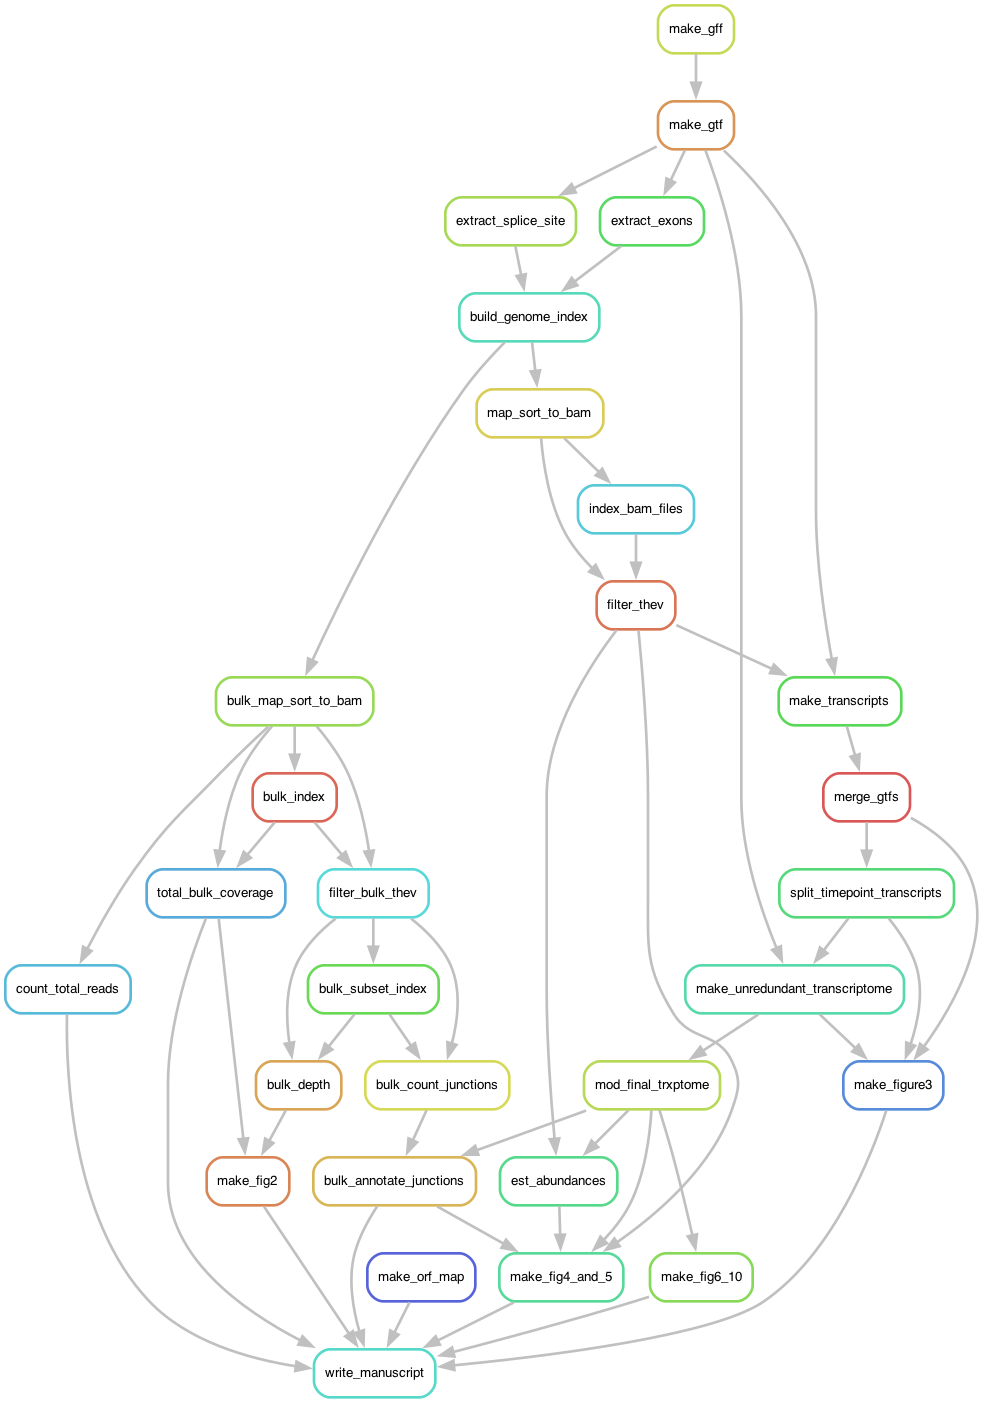
\includegraphics{project_map.png}
\caption{A flowchart of the major steps in the computational analysis
pipeline (\emph{generated with Snakemake})}
\end{figure}

\end{document}
